\documentclass[twoside]{book}

% Packages required by doxygen
\usepackage{fixltx2e}
\usepackage{calc}
\usepackage{doxygen}
\usepackage{graphicx}
\usepackage[utf8]{inputenc}
\usepackage{makeidx}
\usepackage{multicol}
\usepackage{multirow}
\PassOptionsToPackage{warn}{textcomp}
\usepackage{textcomp}
\usepackage[nointegrals]{wasysym}
\usepackage[table]{xcolor}

% NLS support packages
\usepackage[italian]{babel}

% Font selection
\usepackage[T1]{fontenc}
\usepackage{mathptmx}
\usepackage[scaled=.90]{helvet}
\usepackage{courier}
\usepackage{amssymb}
\usepackage{sectsty}
\renewcommand{\familydefault}{\sfdefault}
\allsectionsfont{%
  \fontseries{bc}\selectfont%
  \color{darkgray}%
}
\renewcommand{\DoxyLabelFont}{%
  \fontseries{bc}\selectfont%
  \color{darkgray}%
}
\newcommand{\+}{\discretionary{\mbox{\scriptsize$\hookleftarrow$}}{}{}}

% Page & text layout
\usepackage{geometry}
\geometry{%
  a4paper,%
  top=2.5cm,%
  bottom=2.5cm,%
  left=2.5cm,%
  right=2.5cm%
}
\tolerance=750
\hfuzz=15pt
\hbadness=750
\setlength{\emergencystretch}{15pt}
\setlength{\parindent}{0cm}
\setlength{\parskip}{0.2cm}
\makeatletter
\renewcommand{\paragraph}{%
  \@startsection{paragraph}{4}{0ex}{-1.0ex}{1.0ex}{%
    \normalfont\normalsize\bfseries\SS@parafont%
  }%
}
\renewcommand{\subparagraph}{%
  \@startsection{subparagraph}{5}{0ex}{-1.0ex}{1.0ex}{%
    \normalfont\normalsize\bfseries\SS@subparafont%
  }%
}
\makeatother

% Headers & footers
\usepackage{fancyhdr}
\pagestyle{fancyplain}
\fancyhead[LE]{\fancyplain{}{\bfseries\thepage}}
\fancyhead[CE]{\fancyplain{}{}}
\fancyhead[RE]{\fancyplain{}{\bfseries\leftmark}}
\fancyhead[LO]{\fancyplain{}{\bfseries\rightmark}}
\fancyhead[CO]{\fancyplain{}{}}
\fancyhead[RO]{\fancyplain{}{\bfseries\thepage}}
\fancyfoot[LE]{\fancyplain{}{}}
\fancyfoot[CE]{\fancyplain{}{}}
\fancyfoot[RE]{\fancyplain{}{\bfseries\scriptsize Generato Mer 17 Mag 2017 00\+:07\+:35 per Reed-\/\+Muller Decoder/\+Encoder in V\+H\+D\+L da Doxygen }}
\fancyfoot[LO]{\fancyplain{}{\bfseries\scriptsize Generato Mer 17 Mag 2017 00\+:07\+:35 per Reed-\/\+Muller Decoder/\+Encoder in V\+H\+D\+L da Doxygen }}
\fancyfoot[CO]{\fancyplain{}{}}
\fancyfoot[RO]{\fancyplain{}{}}
\renewcommand{\footrulewidth}{0.4pt}
\renewcommand{\chaptermark}[1]{%
  \markboth{#1}{}%
}
\renewcommand{\sectionmark}[1]{%
  \markright{\thesection\ #1}%
}

% Indices & bibliography
\usepackage{natbib}
\usepackage[titles]{tocloft}
\setcounter{tocdepth}{3}
\setcounter{secnumdepth}{5}
\makeindex

% Hyperlinks (required, but should be loaded last)
\usepackage{ifpdf}
\ifpdf
  \usepackage[pdftex,pagebackref=true]{hyperref}
\else
  \usepackage[ps2pdf,pagebackref=true]{hyperref}
\fi
\hypersetup{%
  colorlinks=true,%
  linkcolor=blue,%
  citecolor=blue,%
  unicode%
}

% Custom commands
\newcommand{\clearemptydoublepage}{%
  \newpage{\pagestyle{empty}\cleardoublepage}%
}


%===== C O N T E N T S =====

\begin{document}

% Titlepage & ToC
\hypersetup{pageanchor=false,
             bookmarks=true,
             bookmarksnumbered=true,
             pdfencoding=unicode
            }
\pagenumbering{roman}
\begin{titlepage}
\vspace*{7cm}
\begin{center}%
{\Large Reed-\/\+Muller Decoder/\+Encoder in V\+H\+D\+L }\\
\vspace*{1cm}
{\large Generato da Doxygen 1.8.8}\\
\vspace*{0.5cm}
{\small Mer 17 Mag 2017 00:07:35}\\
\end{center}
\end{titlepage}
\clearemptydoublepage
\tableofcontents
\clearemptydoublepage
\pagenumbering{arabic}
\hypersetup{pageanchor=true}

%--- Begin generated contents ---
\chapter{Lista dei test}
\label{test}
\hypertarget{test}{}

\begin{DoxyRefList}
\item[\label{test__test000001}%
\hypertarget{test__test000001}{}%
Classe \hyperlink{class_r_m_decoder}{R\+M\+Decoder} ]R\+M(1,m), m=3~\newline
  
\item[\label{test__test000002}%
\hypertarget{test__test000002}{}%
Classe \hyperlink{class_r_m_encoder}{R\+M\+Encoder} ]R\+M(1,m), m=3~\newline
 
\end{DoxyRefList}
\chapter{Indice dei moduli}
\section{Moduli}
Questo è l'elenco di tutti i moduli\+:\begin{DoxyCompactList}
\item \contentsline{section}{R\+M\+Decoder}{\pageref{group___r_m_decoder}}{}
\item \contentsline{section}{Majority\+Voter}{\pageref{group___majority_voter}}{}
\item \contentsline{section}{R\+M\+Encoder}{\pageref{group___r_m_encoder}}{}
\end{DoxyCompactList}

\chapter{Design Unit Index}
\section{Design Unit Hierarchy}
Questo elenco di ereditarietà è ordinato approssimativamente, ma non completamente, in ordine alfabetico\+:\begin{DoxyCompactList}
\item \contentsline{section}{tb\+\_\+\+R\+M\+Decoder}{\pageref{classtb___r_m_decoder}}{}
\begin{DoxyCompactList}
\item \contentsline{section}{R\+M\+Decoder}{\pageref{class_r_m_decoder}}{}
\begin{DoxyCompactList}
\item \contentsline{section}{Generic\+Buffer}{\pageref{class_generic_buffer}}{}
\item \contentsline{section}{Butterfly\+Cell}{\pageref{class_butterfly_cell}}{}
\item \contentsline{section}{majority\+\_\+voter}{\pageref{classmajority__voter}}{}
\begin{DoxyCompactList}
\item \contentsline{section}{parallel\+\_\+counter\+\_\+block}{\pageref{classparallel__counter__block}}{}
\begin{DoxyCompactList}
\item \contentsline{section}{parallel\+\_\+counter\+\_\+4}{\pageref{classparallel__counter__4}}{}
\begin{DoxyCompactList}
\item \contentsline{section}{full\+\_\+adder}{\pageref{classfull__adder}}{}
\end{DoxyCompactList}
\end{DoxyCompactList}
\item \contentsline{section}{generic\+\_\+adder\+\_\+pipelined}{\pageref{classgeneric__adder__pipelined}}{}
\begin{DoxyCompactList}
\item \contentsline{section}{adder\+\_\+block}{\pageref{classadder__block}}{}
\begin{DoxyCompactList}
\item \contentsline{section}{ripple\+\_\+carry\+\_\+adder}{\pageref{classripple__carry__adder}}{}
\item \contentsline{section}{full\+\_\+adder}{\pageref{classfull__adder}}{}
\end{DoxyCompactList}
\item \contentsline{section}{Generic\+Buffer}{\pageref{class_generic_buffer}}{}
\end{DoxyCompactList}
\item \contentsline{section}{generic\+\_\+comparator}{\pageref{classgeneric__comparator}}{}
\begin{DoxyCompactList}
\item \contentsline{section}{comparator2bit}{\pageref{classcomparator2bit}}{}
\end{DoxyCompactList}
\end{DoxyCompactList}
\end{DoxyCompactList}
\end{DoxyCompactList}
\item \contentsline{section}{tb\+\_\+\+R\+M\+Encoder}{\pageref{classtb___r_m_encoder}}{}
\begin{DoxyCompactList}
\item \contentsline{section}{R\+M\+Encoder}{\pageref{class_r_m_encoder}}{}
\end{DoxyCompactList}
\end{DoxyCompactList}

\chapter{Design Unit Index}
\section{Design Unit List}
Here is a list of all design unit members with links to the Entities they belong to\+:\begin{DoxyCompactList}
\item\contentsline{section}{entity \hyperlink{classadder__block}{adder\+\_\+block} \\*Implementazione V\+H\+D\+L \hyperlink{classadder__block_1_1_structural}{Structural} di un generico livello del componente generic\+\_\+adder. Tale livello è costituito da 2$^\wedge$level addizionatori che lavorano in parallelo, di dimensione dipendente dal livello corrente\+: N = number\+\_\+bit\+\_\+for\+\_\+operand + log2(number\+\_\+operand)-\/level-\/1 }{\pageref{classadder__block}}{}
\item\contentsline{section}{architecture \hyperlink{class_generic_buffer_1_1_behavioral}{Behavioral} }{\pageref{class_generic_buffer_1_1_behavioral}}{}
\item\contentsline{section}{architecture \hyperlink{classtb___r_m_decoder_1_1_behavioral}{Behavioral} }{\pageref{classtb___r_m_decoder_1_1_behavioral}}{}
\item\contentsline{section}{architecture \hyperlink{classtb___r_m_encoder_1_1_behavioral}{Behavioral} }{\pageref{classtb___r_m_encoder_1_1_behavioral}}{}
\item\contentsline{section}{entity \hyperlink{class_butterfly_cell}{Butterfly\+Cell} \\*Implementazione V\+H\+D\+L dello swap usato nel decodificatore di Reed-\/\+Muller }{\pageref{class_butterfly_cell}}{}
\item\contentsline{section}{entity \hyperlink{classcomparator2bit}{comparator2bit} \\*Implementazione V\+H\+D\+L Data Flow di un comparatore a 2 bit che tiene conto anche del risutato di un confronto precedente }{\pageref{classcomparator2bit}}{}
\item\contentsline{section}{architecture \hyperlink{classcomparator2bit_1_1_data_flow}{Data\+Flow} }{\pageref{classcomparator2bit_1_1_data_flow}}{}
\item\contentsline{section}{architecture \hyperlink{classfull__adder_1_1_data_flow}{Data\+Flow} }{\pageref{classfull__adder_1_1_data_flow}}{}
\item\contentsline{section}{entity \hyperlink{classfull__adder}{full\+\_\+adder} }{\pageref{classfull__adder}}{}
\item\contentsline{section}{entity \hyperlink{classgeneric__adder__pipelined}{generic\+\_\+adder\+\_\+pipelined} \\*Implementazione V\+H\+D\+L \hyperlink{classgeneric__adder__pipelined_1_1_structural}{Structural} di un addizionatore generico pipelined \+: M operandi di N bit }{\pageref{classgeneric__adder__pipelined}}{}
\item\contentsline{section}{entity \hyperlink{classgeneric__comparator}{generic\+\_\+comparator} \\*Implementazione V\+H\+D\+L \hyperlink{classgeneric__comparator_1_1_structural}{Structural} di un generico comparatore a maggioranza di due stringhe di width bit. Tale implementazione genera una catena di \char`\"{}width\char`\"{} comparatori a 2 bit }{\pageref{classgeneric__comparator}}{}
\item\contentsline{section}{entity \hyperlink{class_generic_buffer}{Generic\+Buffer} \\*Registro di dimensione generica }{\pageref{class_generic_buffer}}{}
\item\contentsline{section}{entity \hyperlink{classmajority__voter}{majority\+\_\+voter} \\*Implementazione V\+H\+D\+L \hyperlink{classmajority__voter_1_1_structural}{Structural} del majority voter }{\pageref{classmajority__voter}}{}
\item\contentsline{section}{entity \hyperlink{classparallel__counter__4}{parallel\+\_\+counter\+\_\+4} }{\pageref{classparallel__counter__4}}{}
\item\contentsline{section}{entity \hyperlink{classparallel__counter__block}{parallel\+\_\+counter\+\_\+block} \\*Implementazione V\+H\+D\+L \hyperlink{classparallel__counter__block_1_1_structural}{Structural} del Modulo 1 \+: genera width/4 contatori paralleli a 4 bit. Data una stringa di input di width bit, multipla di 4, assegna a ogni contatore un nibble. Ogni contatore parallelo a 4 bit codifica in binario il numero di 1 presente nel nibble di competenza }{\pageref{classparallel__counter__block}}{}
\item\contentsline{section}{entity \hyperlink{classripple__carry__adder}{ripple\+\_\+carry\+\_\+adder} \\*Implementazione V\+H\+D\+L Structural di un Ripple Carry Adder generico a N bit }{\pageref{classripple__carry__adder}}{}
\item\contentsline{section}{entity \hyperlink{class_r_m_decoder}{R\+M\+Decoder} \\*Implementazione V\+H\+D\+L del decodificatore per codici di Reed-\/\+Muller(1,m) }{\pageref{class_r_m_decoder}}{}
\item\contentsline{section}{entity \hyperlink{class_r_m_encoder}{R\+M\+Encoder} \\*Implementazione V\+H\+D\+L del codificatore per codici di Reed-\/\+Muller(1,m) }{\pageref{class_r_m_encoder}}{}
\item\contentsline{section}{architecture \hyperlink{classadder__block_1_1_structural}{Structural} }{\pageref{classadder__block_1_1_structural}}{}
\item\contentsline{section}{architecture \hyperlink{classparallel__counter__4_1_1_structural}{Structural} }{\pageref{classparallel__counter__4_1_1_structural}}{}
\item\contentsline{section}{architecture \hyperlink{class_butterfly_cell_1_1_structural}{Structural} }{\pageref{class_butterfly_cell_1_1_structural}}{}
\item\contentsline{section}{architecture \hyperlink{classripple__carry__adder_1_1structural}{structural} }{\pageref{classripple__carry__adder_1_1structural}}{}
\item\contentsline{section}{architecture \hyperlink{class_r_m_decoder_1_1_structural}{Structural} }{\pageref{class_r_m_decoder_1_1_structural}}{}
\item\contentsline{section}{architecture \hyperlink{class_r_m_encoder_1_1_structural}{Structural} }{\pageref{class_r_m_encoder_1_1_structural}}{}
\item\contentsline{section}{architecture \hyperlink{classgeneric__comparator_1_1_structural}{Structural} }{\pageref{classgeneric__comparator_1_1_structural}}{}
\item\contentsline{section}{architecture \hyperlink{classgeneric__adder__pipelined_1_1_structural}{Structural} }{\pageref{classgeneric__adder__pipelined_1_1_structural}}{}
\item\contentsline{section}{architecture \hyperlink{classmajority__voter_1_1_structural}{Structural} }{\pageref{classmajority__voter_1_1_structural}}{}
\item\contentsline{section}{architecture \hyperlink{classparallel__counter__block_1_1_structural}{Structural} }{\pageref{classparallel__counter__block_1_1_structural}}{}
\item\contentsline{section}{entity \hyperlink{classtb___r_m_decoder}{tb\+\_\+\+R\+M\+Decoder} }{\pageref{classtb___r_m_decoder}}{}
\item\contentsline{section}{entity \hyperlink{classtb___r_m_encoder}{tb\+\_\+\+R\+M\+Encoder} }{\pageref{classtb___r_m_encoder}}{}
\end{DoxyCompactList}

\chapter{Indice dei file}
\section{Elenco dei file}
Questo è un elenco dei file documentati con una loro breve descrizione\+:\begin{DoxyCompactList}
\item\contentsline{section}{R\+M\+Decoder/\hyperlink{_butterfly_cell_8vhd}{Butterfly\+Cell.\+vhd} }{\pageref{_butterfly_cell_8vhd}}{}
\item\contentsline{section}{R\+M\+Decoder/\hyperlink{_r_m_decoder_8vhd}{R\+M\+Decoder.\+vhd} }{\pageref{_r_m_decoder_8vhd}}{}
\item\contentsline{section}{R\+M\+Decoder/\+Majority\+Voter/\hyperlink{adder__block_8vhd}{adder\+\_\+block.\+vhd} }{\pageref{adder__block_8vhd}}{}
\item\contentsline{section}{R\+M\+Decoder/\+Majority\+Voter/\hyperlink{comparator2bit_8vhd}{comparator2bit.\+vhd} }{\pageref{comparator2bit_8vhd}}{}
\item\contentsline{section}{R\+M\+Decoder/\+Majority\+Voter/\hyperlink{full__adder_8vhd}{full\+\_\+adder.\+vhd} }{\pageref{full__adder_8vhd}}{}
\item\contentsline{section}{R\+M\+Decoder/\+Majority\+Voter/\hyperlink{generic__adder__pipelined_8vhd}{generic\+\_\+adder\+\_\+pipelined.\+vhd} }{\pageref{generic__adder__pipelined_8vhd}}{}
\item\contentsline{section}{R\+M\+Decoder/\+Majority\+Voter/\hyperlink{generic__comparator_8vhd}{generic\+\_\+comparator.\+vhd} }{\pageref{generic__comparator_8vhd}}{}
\item\contentsline{section}{R\+M\+Decoder/\+Majority\+Voter/\hyperlink{majority__voter_8vhd}{majority\+\_\+voter.\+vhd} }{\pageref{majority__voter_8vhd}}{}
\item\contentsline{section}{R\+M\+Decoder/\+Majority\+Voter/\hyperlink{parallel__counter__4_8vhd}{parallel\+\_\+counter\+\_\+4.\+vhd} }{\pageref{parallel__counter__4_8vhd}}{}
\item\contentsline{section}{R\+M\+Decoder/\+Majority\+Voter/\hyperlink{parallel__counter__block_8vhd}{parallel\+\_\+counter\+\_\+block.\+vhd} }{\pageref{parallel__counter__block_8vhd}}{}
\item\contentsline{section}{R\+M\+Decoder/\+Majority\+Voter/\hyperlink{ripple__carry__adder_8vhd}{ripple\+\_\+carry\+\_\+adder.\+vhd} }{\pageref{ripple__carry__adder_8vhd}}{}
\item\contentsline{section}{R\+M\+Encoder/\hyperlink{_r_m_encoder_8vhd}{R\+M\+Encoder.\+vhd} }{\pageref{_r_m_encoder_8vhd}}{}
\end{DoxyCompactList}

\chapter{Documentazione dei moduli}
\hypertarget{group___r_m_decoder}{\section{R\+M\+Decoder}
\label{group___r_m_decoder}\index{R\+M\+Decoder@{R\+M\+Decoder}}
}
\subsection*{Entities}
\begin{DoxyCompactItemize}
\item 
\hyperlink{class_butterfly_cell}{Butterfly\+Cell} entity
\begin{DoxyCompactList}\small\item\em implementazione V\+H\+D\+L dello swap usato nel decodificatore di Reed-\/\+Muller \end{DoxyCompactList}\item 
\hyperlink{class_butterfly_cell_1_1_structural}{Structural} architecture
\item 
\hyperlink{class_generic_buffer}{Generic\+Buffer} entity
\begin{DoxyCompactList}\small\item\em Registro di dimensione generica. \end{DoxyCompactList}\item 
\hyperlink{class_generic_buffer_1_1_behavioral}{Behavioral} architecture
\item 
\hyperlink{class_r_m_decoder}{R\+M\+Decoder} entity
\begin{DoxyCompactList}\small\item\em Implementazione V\+H\+D\+L del decodificatore per codici di Reed-\/\+Muller(1,m) \end{DoxyCompactList}\item 
\hyperlink{classtb___r_m_decoder}{tb\+\_\+\+R\+M\+Decoder} entity
\end{DoxyCompactItemize}
\subsection*{Processes}
 \begin{DoxyCompactItemize}
\item 
\hypertarget{group___r_m_decoder_ga2ee480e118ca2b3fccf26139a66e84ad}{\hyperlink{group___r_m_decoder_ga2ee480e118ca2b3fccf26139a66e84ad}{P\+R\+O\+C\+E\+S\+S\+\_\+0}{\bfseries  ( {\bfseries \textcolor{vhdlchar}{clock}\textcolor{vhdlchar}{ }} , {\bfseries \textcolor{vhdlchar}{reset\+\_\+n}\textcolor{vhdlchar}{ }} , {\bfseries \textcolor{vhdlchar}{load}\textcolor{vhdlchar}{ }} , {\bfseries \textcolor{vhdlchar}{data\+\_\+in}\textcolor{vhdlchar}{ }} )}}\label{group___r_m_decoder_ga2ee480e118ca2b3fccf26139a66e84ad}

\item 
\hypertarget{group___r_m_decoder_gaee7e8b077315d73d2c245522dd7ba9a8}{\hyperlink{group___r_m_decoder_gaee7e8b077315d73d2c245522dd7ba9a8}{stim\+\_\+process}{\bfseries  (  )}}\label{group___r_m_decoder_gaee7e8b077315d73d2c245522dd7ba9a8}

\end{DoxyCompactItemize}
\subsection*{Libraries}
 \begin{DoxyCompactItemize}
\item 
\hypertarget{group___r_m_decoder_ga0a6af6eef40212dbaf130d57ce711256}{\hyperlink{group___r_m_decoder_ga0a6af6eef40212dbaf130d57ce711256}{ieee} }\label{group___r_m_decoder_ga0a6af6eef40212dbaf130d57ce711256}

\end{DoxyCompactItemize}
\subsection*{Use Clauses}
 \begin{DoxyCompactItemize}
\item 
\hypertarget{group___r_m_decoder_gacd03516902501cd1c7296a98e22c6fcb}{\hyperlink{group___r_m_decoder_gacd03516902501cd1c7296a98e22c6fcb}{std\+\_\+logic\+\_\+1164}   }\label{group___r_m_decoder_gacd03516902501cd1c7296a98e22c6fcb}

\item 
\hypertarget{group___r_m_decoder_gacd03516902501cd1c7296a98e22c6fcb}{\hyperlink{group___r_m_decoder_gacd03516902501cd1c7296a98e22c6fcb}{std\+\_\+logic\+\_\+1164}   }\label{group___r_m_decoder_gacd03516902501cd1c7296a98e22c6fcb}

\item 
\hypertarget{group___r_m_decoder_gacd03516902501cd1c7296a98e22c6fcb}{\hyperlink{group___r_m_decoder_gacd03516902501cd1c7296a98e22c6fcb}{std\+\_\+logic\+\_\+1164}   }\label{group___r_m_decoder_gacd03516902501cd1c7296a98e22c6fcb}

\item 
\hypertarget{group___r_m_decoder_ga2edc34402b573437d5f25fa90ba4013e}{\hyperlink{group___r_m_decoder_ga2edc34402b573437d5f25fa90ba4013e}{numeric\+\_\+std}   }\label{group___r_m_decoder_ga2edc34402b573437d5f25fa90ba4013e}

\item 
\hypertarget{group___r_m_decoder_gacd03516902501cd1c7296a98e22c6fcb}{\hyperlink{group___r_m_decoder_gacd03516902501cd1c7296a98e22c6fcb}{std\+\_\+logic\+\_\+1164}   }\label{group___r_m_decoder_gacd03516902501cd1c7296a98e22c6fcb}

\end{DoxyCompactItemize}
\subsection*{Components}
 \begin{DoxyCompactItemize}
\item 
\hypertarget{group___r_m_decoder_ga26754353fa942392a9799290b42c41c7}{\hyperlink{group___r_m_decoder_ga26754353fa942392a9799290b42c41c7}{Generic\+Buffer}  {\bfseries }  }\label{group___r_m_decoder_ga26754353fa942392a9799290b42c41c7}

\item 
\hypertarget{group___r_m_decoder_ga78b932f12128347f9985cb5f28b83a4d}{\hyperlink{group___r_m_decoder_ga78b932f12128347f9985cb5f28b83a4d}{Butterfly\+Cell}  {\bfseries }  }\label{group___r_m_decoder_ga78b932f12128347f9985cb5f28b83a4d}

\item 
\hypertarget{group___r_m_decoder_gadabe01418633fc7a7416a2b27787c4f5}{\hyperlink{group___r_m_decoder_gadabe01418633fc7a7416a2b27787c4f5}{majority\+\_\+voter}  {\bfseries }  }\label{group___r_m_decoder_gadabe01418633fc7a7416a2b27787c4f5}

\item 
\hypertarget{group___r_m_decoder_gaa428b5ac9b6611fe96abf435a343d47c}{\hyperlink{group___r_m_decoder_gaa428b5ac9b6611fe96abf435a343d47c}{R\+M\+Decoder}  {\bfseries }  }\label{group___r_m_decoder_gaa428b5ac9b6611fe96abf435a343d47c}

\end{DoxyCompactItemize}
\subsection*{Constants}
 \begin{DoxyCompactItemize}
\item 
\hypertarget{group___r_m_decoder_gaa60d5ca93133573b9fb3e8cc51520aa1}{\hyperlink{group___r_m_decoder_gaa60d5ca93133573b9fb3e8cc51520aa1}{zero} {\bfseries \textcolor{vhdlchar}{std\+\_\+logic\+\_\+vector}\textcolor{vhdlchar}{ }\textcolor{vhdlchar}{(}\textcolor{vhdlchar}{ }\textcolor{vhdlchar}{ } \textcolor{vhdldigit}{2} \textcolor{vhdlchar}{$\ast$}\textcolor{vhdlchar}{$\ast$}\textcolor{vhdlchar}{ }\textcolor{vhdlchar}{ }\textcolor{vhdlchar}{ }\textcolor{vhdlchar}{m}\textcolor{vhdlchar}{-\/}\textcolor{vhdlchar}{ } \textcolor{vhdldigit}{1} \textcolor{vhdlchar}{ }\textcolor{vhdlchar}{downto}\textcolor{vhdlchar}{ }\textcolor{vhdlchar}{ } \textcolor{vhdldigit}{0} \textcolor{vhdlchar}{ }\textcolor{vhdlchar}{)}\textcolor{vhdlchar}{ }\textcolor{vhdlchar}{ }\textcolor{vhdlchar}{ }\textcolor{vhdlchar}{\+:}\textcolor{vhdlchar}{=}\textcolor{vhdlchar}{ }\textcolor{vhdlchar}{(}\textcolor{vhdlchar}{ }\textcolor{vhdlchar}{ }\textcolor{vhdlchar}{others}\textcolor{vhdlchar}{ }\textcolor{vhdlchar}{ }\textcolor{vhdlchar}{=}\textcolor{vhdlchar}{ }\textcolor{vhdlchar}{$>$}\textcolor{vhdlchar}{ }\textcolor{vhdlchar}{'}\textcolor{vhdlchar}{ } \textcolor{vhdldigit}{0} \textcolor{vhdlchar}{ }\textcolor{vhdlchar}{'}\textcolor{vhdlchar}{ }\textcolor{vhdlchar}{)}\textcolor{vhdlchar}{ }} }\label{group___r_m_decoder_gaa60d5ca93133573b9fb3e8cc51520aa1}

\item 
\hypertarget{group___r_m_decoder_ga66500af96850e5a149ace8e4005a489a}{\hyperlink{group___r_m_decoder_ga66500af96850e5a149ace8e4005a489a}{m} {\bfseries \textcolor{vhdlchar}{natural}\textcolor{vhdlchar}{ }\textcolor{vhdlchar}{ }\textcolor{vhdlchar}{\+:}\textcolor{vhdlchar}{=}\textcolor{vhdlchar}{ }\textcolor{vhdlchar}{ } \textcolor{vhdldigit}{4} \textcolor{vhdlchar}{ }} }\label{group___r_m_decoder_ga66500af96850e5a149ace8e4005a489a}

\item 
\hypertarget{group___r_m_decoder_ga9fb080b7379b7a2f64508f2e5c5f0cba}{\hyperlink{group___r_m_decoder_ga9fb080b7379b7a2f64508f2e5c5f0cba}{encoded} {\bfseries \textcolor{vhdlchar}{matrix}\textcolor{vhdlchar}{ }\textcolor{vhdlchar}{(}\textcolor{vhdlchar}{ }\textcolor{vhdlchar}{ } \textcolor{vhdldigit}{0} \textcolor{vhdlchar}{ }\textcolor{vhdlchar}{to}\textcolor{vhdlchar}{ }\textcolor{vhdlchar}{ } \textcolor{vhdldigit}{2} \textcolor{vhdlchar}{$\ast$}\textcolor{vhdlchar}{$\ast$}\textcolor{vhdlchar}{ }\textcolor{vhdlchar}{(}\textcolor{vhdlchar}{ }\textcolor{vhdlchar}{ }\textcolor{vhdlchar}{ }\textcolor{vhdlchar}{ }\textcolor{vhdlchar}{m}\textcolor{vhdlchar}{+}\textcolor{vhdlchar}{ } \textcolor{vhdldigit}{1} \textcolor{vhdlchar}{ }\textcolor{vhdlchar}{)}\textcolor{vhdlchar}{ }\textcolor{vhdlchar}{-\/}\textcolor{vhdlchar}{ } \textcolor{vhdldigit}{1} \textcolor{vhdlchar}{ }\textcolor{vhdlchar}{)}\textcolor{vhdlchar}{ }\textcolor{vhdlchar}{ }\textcolor{vhdlchar}{ }\textcolor{vhdlchar}{\+:}\textcolor{vhdlchar}{=}\textcolor{vhdlchar}{ }\textcolor{vhdlchar}{(}\textcolor{vhdlchar}{ }\textcolor{vhdlchar}{(}\textcolor{vhdlchar}{ }\textcolor{vhdlchar}{ }\textcolor{vhdlchar}{x}\textcolor{vhdlchar}{ }\textcolor{keyword}{\char`\"{} 0000 \char`\"{}}\textcolor{vhdlchar}{ }\textcolor{vhdlchar}{)}\textcolor{vhdlchar}{ }\textcolor{vhdlchar}{,}\textcolor{vhdlchar}{ }\textcolor{vhdlchar}{(}\textcolor{vhdlchar}{ }\textcolor{vhdlchar}{ }\textcolor{vhdlchar}{x}\textcolor{vhdlchar}{ }\textcolor{keyword}{\char`\"{} 5555 \char`\"{}}\textcolor{vhdlchar}{ }\textcolor{vhdlchar}{)}\textcolor{vhdlchar}{ }\textcolor{vhdlchar}{,}\textcolor{vhdlchar}{ }\textcolor{vhdlchar}{(}\textcolor{vhdlchar}{ }\textcolor{vhdlchar}{ }\textcolor{vhdlchar}{x}\textcolor{vhdlchar}{ }\textcolor{keyword}{\char`\"{} 3333 \char`\"{}}\textcolor{vhdlchar}{ }\textcolor{vhdlchar}{)}\textcolor{vhdlchar}{ }\textcolor{vhdlchar}{,}\textcolor{vhdlchar}{ }\textcolor{vhdlchar}{(}\textcolor{vhdlchar}{ }\textcolor{vhdlchar}{ }\textcolor{vhdlchar}{x}\textcolor{vhdlchar}{ }\textcolor{keyword}{\char`\"{} 6666 \char`\"{}}\textcolor{vhdlchar}{ }\textcolor{vhdlchar}{)}\textcolor{vhdlchar}{ }\textcolor{vhdlchar}{,}\textcolor{vhdlchar}{ }\textcolor{vhdlchar}{(}\textcolor{vhdlchar}{ }\textcolor{vhdlchar}{ }\textcolor{vhdlchar}{x}\textcolor{vhdlchar}{ }\textcolor{keyword}{\char`\"{} 0f0f \char`\"{}}\textcolor{vhdlchar}{ }\textcolor{vhdlchar}{)}\textcolor{vhdlchar}{ }\textcolor{vhdlchar}{,}\textcolor{vhdlchar}{ }\textcolor{vhdlchar}{(}\textcolor{vhdlchar}{ }\textcolor{vhdlchar}{ }\textcolor{vhdlchar}{x}\textcolor{vhdlchar}{ }\textcolor{keyword}{\char`\"{} 5a5a \char`\"{}}\textcolor{vhdlchar}{ }\textcolor{vhdlchar}{)}\textcolor{vhdlchar}{ }\textcolor{vhdlchar}{,}\textcolor{vhdlchar}{ }\textcolor{vhdlchar}{(}\textcolor{vhdlchar}{ }\textcolor{vhdlchar}{ }\textcolor{vhdlchar}{x}\textcolor{vhdlchar}{ }\textcolor{keyword}{\char`\"{} 3c3c \char`\"{}}\textcolor{vhdlchar}{ }\textcolor{vhdlchar}{)}\textcolor{vhdlchar}{ }\textcolor{vhdlchar}{,}\textcolor{vhdlchar}{ }\textcolor{vhdlchar}{(}\textcolor{vhdlchar}{ }\textcolor{vhdlchar}{ }\textcolor{vhdlchar}{x}\textcolor{vhdlchar}{ }\textcolor{keyword}{\char`\"{} 6969 \char`\"{}}\textcolor{vhdlchar}{ }\textcolor{vhdlchar}{)}\textcolor{vhdlchar}{ }\textcolor{vhdlchar}{,}\textcolor{vhdlchar}{ }\textcolor{vhdlchar}{(}\textcolor{vhdlchar}{ }\textcolor{vhdlchar}{ }\textcolor{vhdlchar}{x}\textcolor{vhdlchar}{ }\textcolor{keyword}{\char`\"{} 00ff \char`\"{}}\textcolor{vhdlchar}{ }\textcolor{vhdlchar}{)}\textcolor{vhdlchar}{ }\textcolor{vhdlchar}{,}\textcolor{vhdlchar}{ }\textcolor{vhdlchar}{(}\textcolor{vhdlchar}{ }\textcolor{vhdlchar}{ }\textcolor{vhdlchar}{x}\textcolor{vhdlchar}{ }\textcolor{keyword}{\char`\"{} 55aa \char`\"{}}\textcolor{vhdlchar}{ }\textcolor{vhdlchar}{)}\textcolor{vhdlchar}{ }\textcolor{vhdlchar}{,}\textcolor{vhdlchar}{ }\textcolor{vhdlchar}{(}\textcolor{vhdlchar}{ }\textcolor{vhdlchar}{ }\textcolor{vhdlchar}{x}\textcolor{vhdlchar}{ }\textcolor{keyword}{\char`\"{} 33cc \char`\"{}}\textcolor{vhdlchar}{ }\textcolor{vhdlchar}{)}\textcolor{vhdlchar}{ }\textcolor{vhdlchar}{,}\textcolor{vhdlchar}{ }\textcolor{vhdlchar}{(}\textcolor{vhdlchar}{ }\textcolor{vhdlchar}{ }\textcolor{vhdlchar}{x}\textcolor{vhdlchar}{ }\textcolor{keyword}{\char`\"{} 6699 \char`\"{}}\textcolor{vhdlchar}{ }\textcolor{vhdlchar}{)}\textcolor{vhdlchar}{ }\textcolor{vhdlchar}{,}\textcolor{vhdlchar}{ }\textcolor{vhdlchar}{(}\textcolor{vhdlchar}{ }\textcolor{vhdlchar}{ }\textcolor{vhdlchar}{x}\textcolor{vhdlchar}{ }\textcolor{keyword}{\char`\"{} 0ff0 \char`\"{}}\textcolor{vhdlchar}{ }\textcolor{vhdlchar}{)}\textcolor{vhdlchar}{ }\textcolor{vhdlchar}{,}\textcolor{vhdlchar}{ }\textcolor{vhdlchar}{(}\textcolor{vhdlchar}{ }\textcolor{vhdlchar}{ }\textcolor{vhdlchar}{x}\textcolor{vhdlchar}{ }\textcolor{keyword}{\char`\"{} 5aa5 \char`\"{}}\textcolor{vhdlchar}{ }\textcolor{vhdlchar}{)}\textcolor{vhdlchar}{ }\textcolor{vhdlchar}{,}\textcolor{vhdlchar}{ }\textcolor{vhdlchar}{(}\textcolor{vhdlchar}{ }\textcolor{vhdlchar}{ }\textcolor{vhdlchar}{x}\textcolor{vhdlchar}{ }\textcolor{keyword}{\char`\"{} 3cc3 \char`\"{}}\textcolor{vhdlchar}{ }\textcolor{vhdlchar}{)}\textcolor{vhdlchar}{ }\textcolor{vhdlchar}{,}\textcolor{vhdlchar}{ }\textcolor{vhdlchar}{(}\textcolor{vhdlchar}{ }\textcolor{vhdlchar}{ }\textcolor{vhdlchar}{x}\textcolor{vhdlchar}{ }\textcolor{keyword}{\char`\"{} 6996 \char`\"{}}\textcolor{vhdlchar}{ }\textcolor{vhdlchar}{)}\textcolor{vhdlchar}{ }\textcolor{vhdlchar}{,}\textcolor{vhdlchar}{ }\textcolor{vhdlchar}{(}\textcolor{vhdlchar}{ }\textcolor{vhdlchar}{ }\textcolor{vhdlchar}{x}\textcolor{vhdlchar}{ }\textcolor{keyword}{\char`\"{} ffff \char`\"{}}\textcolor{vhdlchar}{ }\textcolor{vhdlchar}{)}\textcolor{vhdlchar}{ }\textcolor{vhdlchar}{,}\textcolor{vhdlchar}{ }\textcolor{vhdlchar}{(}\textcolor{vhdlchar}{ }\textcolor{vhdlchar}{ }\textcolor{vhdlchar}{x}\textcolor{vhdlchar}{ }\textcolor{keyword}{\char`\"{} aaaa \char`\"{}}\textcolor{vhdlchar}{ }\textcolor{vhdlchar}{)}\textcolor{vhdlchar}{ }\textcolor{vhdlchar}{,}\textcolor{vhdlchar}{ }\textcolor{vhdlchar}{(}\textcolor{vhdlchar}{ }\textcolor{vhdlchar}{ }\textcolor{vhdlchar}{x}\textcolor{vhdlchar}{ }\textcolor{keyword}{\char`\"{} cccc \char`\"{}}\textcolor{vhdlchar}{ }\textcolor{vhdlchar}{)}\textcolor{vhdlchar}{ }\textcolor{vhdlchar}{,}\textcolor{vhdlchar}{ }\textcolor{vhdlchar}{(}\textcolor{vhdlchar}{ }\textcolor{vhdlchar}{ }\textcolor{vhdlchar}{x}\textcolor{vhdlchar}{ }\textcolor{keyword}{\char`\"{} 9999 \char`\"{}}\textcolor{vhdlchar}{ }\textcolor{vhdlchar}{)}\textcolor{vhdlchar}{ }\textcolor{vhdlchar}{,}\textcolor{vhdlchar}{ }\textcolor{vhdlchar}{(}\textcolor{vhdlchar}{ }\textcolor{vhdlchar}{ }\textcolor{vhdlchar}{x}\textcolor{vhdlchar}{ }\textcolor{keyword}{\char`\"{} f0f0 \char`\"{}}\textcolor{vhdlchar}{ }\textcolor{vhdlchar}{)}\textcolor{vhdlchar}{ }\textcolor{vhdlchar}{,}\textcolor{vhdlchar}{ }\textcolor{vhdlchar}{(}\textcolor{vhdlchar}{ }\textcolor{vhdlchar}{ }\textcolor{vhdlchar}{x}\textcolor{vhdlchar}{ }\textcolor{keyword}{\char`\"{} a5a5 \char`\"{}}\textcolor{vhdlchar}{ }\textcolor{vhdlchar}{)}\textcolor{vhdlchar}{ }\textcolor{vhdlchar}{,}\textcolor{vhdlchar}{ }\textcolor{vhdlchar}{(}\textcolor{vhdlchar}{ }\textcolor{vhdlchar}{ }\textcolor{vhdlchar}{x}\textcolor{vhdlchar}{ }\textcolor{keyword}{\char`\"{} c3c3 \char`\"{}}\textcolor{vhdlchar}{ }\textcolor{vhdlchar}{)}\textcolor{vhdlchar}{ }\textcolor{vhdlchar}{,}\textcolor{vhdlchar}{ }\textcolor{vhdlchar}{(}\textcolor{vhdlchar}{ }\textcolor{vhdlchar}{ }\textcolor{vhdlchar}{x}\textcolor{vhdlchar}{ }\textcolor{keyword}{\char`\"{} 9696 \char`\"{}}\textcolor{vhdlchar}{ }\textcolor{vhdlchar}{)}\textcolor{vhdlchar}{ }\textcolor{vhdlchar}{,}\textcolor{vhdlchar}{ }\textcolor{vhdlchar}{(}\textcolor{vhdlchar}{ }\textcolor{vhdlchar}{ }\textcolor{vhdlchar}{x}\textcolor{vhdlchar}{ }\textcolor{keyword}{\char`\"{} ff00 \char`\"{}}\textcolor{vhdlchar}{ }\textcolor{vhdlchar}{)}\textcolor{vhdlchar}{ }\textcolor{vhdlchar}{,}\textcolor{vhdlchar}{ }\textcolor{vhdlchar}{(}\textcolor{vhdlchar}{ }\textcolor{vhdlchar}{ }\textcolor{vhdlchar}{x}\textcolor{vhdlchar}{ }\textcolor{keyword}{\char`\"{} aa55 \char`\"{}}\textcolor{vhdlchar}{ }\textcolor{vhdlchar}{)}\textcolor{vhdlchar}{ }\textcolor{vhdlchar}{,}\textcolor{vhdlchar}{ }\textcolor{vhdlchar}{(}\textcolor{vhdlchar}{ }\textcolor{vhdlchar}{ }\textcolor{vhdlchar}{x}\textcolor{vhdlchar}{ }\textcolor{keyword}{\char`\"{} cc33 \char`\"{}}\textcolor{vhdlchar}{ }\textcolor{vhdlchar}{)}\textcolor{vhdlchar}{ }\textcolor{vhdlchar}{,}\textcolor{vhdlchar}{ }\textcolor{vhdlchar}{(}\textcolor{vhdlchar}{ }\textcolor{vhdlchar}{ }\textcolor{vhdlchar}{x}\textcolor{vhdlchar}{ }\textcolor{keyword}{\char`\"{} 9966 \char`\"{}}\textcolor{vhdlchar}{ }\textcolor{vhdlchar}{)}\textcolor{vhdlchar}{ }\textcolor{vhdlchar}{,}\textcolor{vhdlchar}{ }\textcolor{vhdlchar}{(}\textcolor{vhdlchar}{ }\textcolor{vhdlchar}{ }\textcolor{vhdlchar}{x}\textcolor{vhdlchar}{ }\textcolor{keyword}{\char`\"{} f00f \char`\"{}}\textcolor{vhdlchar}{ }\textcolor{vhdlchar}{)}\textcolor{vhdlchar}{ }\textcolor{vhdlchar}{,}\textcolor{vhdlchar}{ }\textcolor{vhdlchar}{(}\textcolor{vhdlchar}{ }\textcolor{vhdlchar}{ }\textcolor{vhdlchar}{x}\textcolor{vhdlchar}{ }\textcolor{keyword}{\char`\"{} a55a \char`\"{}}\textcolor{vhdlchar}{ }\textcolor{vhdlchar}{)}\textcolor{vhdlchar}{ }\textcolor{vhdlchar}{,}\textcolor{vhdlchar}{ }\textcolor{vhdlchar}{(}\textcolor{vhdlchar}{ }\textcolor{vhdlchar}{ }\textcolor{vhdlchar}{x}\textcolor{vhdlchar}{ }\textcolor{keyword}{\char`\"{} c33c \char`\"{}}\textcolor{vhdlchar}{ }\textcolor{vhdlchar}{)}\textcolor{vhdlchar}{ }\textcolor{vhdlchar}{,}\textcolor{vhdlchar}{ }\textcolor{vhdlchar}{(}\textcolor{vhdlchar}{ }\textcolor{vhdlchar}{ }\textcolor{vhdlchar}{x}\textcolor{vhdlchar}{ }\textcolor{keyword}{\char`\"{} 9669 \char`\"{}}\textcolor{vhdlchar}{ }\textcolor{vhdlchar}{)}\textcolor{vhdlchar}{ }} }\label{group___r_m_decoder_ga9fb080b7379b7a2f64508f2e5c5f0cba}

\item 
\hypertarget{group___r_m_decoder_ga56b871d5221ff49e502a0ac86ad875ea}{\hyperlink{group___r_m_decoder_ga56b871d5221ff49e502a0ac86ad875ea}{clock\+\_\+period} {\bfseries \textcolor{vhdlchar}{time}\textcolor{vhdlchar}{ }\textcolor{vhdlchar}{ }\textcolor{vhdlchar}{\+:}\textcolor{vhdlchar}{=}\textcolor{vhdlchar}{ }\textcolor{vhdlchar}{ }\textcolor{vhdlchar}{ } \textcolor{vhdldigit}{10} \textcolor{vhdlchar}{ }\textcolor{vhdlchar}{ns}\textcolor{vhdlchar}{ }} }\label{group___r_m_decoder_ga56b871d5221ff49e502a0ac86ad875ea}

\item 
\hypertarget{group___r_m_decoder_ga57b43bd889cdfa2bf9597490517dd675}{\hyperlink{group___r_m_decoder_ga57b43bd889cdfa2bf9597490517dd675}{generator\+\_\+matrix\+\_\+01} {\bfseries \textcolor{vhdlchar}{boolean}\textcolor{vhdlchar}{ }\textcolor{vhdlchar}{ }\textcolor{vhdlchar}{\+:}\textcolor{vhdlchar}{=}\textcolor{vhdlchar}{ }\textcolor{vhdlchar}{ }\textcolor{vhdlchar}{ }\textcolor{vhdlchar}{ }\textcolor{vhdlchar}{true}\textcolor{vhdlchar}{ }} }\label{group___r_m_decoder_ga57b43bd889cdfa2bf9597490517dd675}

\end{DoxyCompactItemize}
\subsection*{Types}
 \begin{DoxyCompactItemize}
\item 
\hypertarget{group___r_m_decoder_ga88b1f19c6b66040e3719ce83a8832903}{{\bfseries \hyperlink{group___r_m_decoder_ga88b1f19c6b66040e3719ce83a8832903}{std\+\_\+logic\+\_\+matrix1}{\bfseries \textcolor{vhdlchar}{array}\textcolor{vhdlchar}{ }\textcolor{vhdlchar}{(}\textcolor{vhdlchar}{ }\textcolor{vhdlchar}{natural}\textcolor{vhdlchar}{ }\textcolor{vhdlchar}{range}\textcolor{vhdlchar}{ }\textcolor{vhdlchar}{$<$$>$}\textcolor{vhdlchar}{ }\textcolor{vhdlchar}{)}\textcolor{vhdlchar}{ }\textcolor{vhdlchar}{ }\textcolor{vhdlchar}{of}\textcolor{vhdlchar}{ }\textcolor{vhdlchar}{std\+\_\+logic\+\_\+vector}\textcolor{vhdlchar}{ }\textcolor{vhdlchar}{(}\textcolor{vhdlchar}{ }\textcolor{vhdlchar}{ } \textcolor{vhdldigit}{2} \textcolor{vhdlchar}{$\ast$}\textcolor{vhdlchar}{$\ast$}\textcolor{vhdlchar}{ }\textcolor{vhdlchar}{ }\textcolor{vhdlchar}{ }\textcolor{vhdlchar}{m}\textcolor{vhdlchar}{-\/}\textcolor{vhdlchar}{ } \textcolor{vhdldigit}{1} \textcolor{vhdlchar}{ }\textcolor{vhdlchar}{downto}\textcolor{vhdlchar}{ }\textcolor{vhdlchar}{ } \textcolor{vhdldigit}{0} \textcolor{vhdlchar}{ }\textcolor{vhdlchar}{)}\textcolor{vhdlchar}{ }}} }\label{group___r_m_decoder_ga88b1f19c6b66040e3719ce83a8832903}

\item 
\hypertarget{group___r_m_decoder_ga276be67840f4fbd1d23853217df170f2}{{\bfseries \hyperlink{group___r_m_decoder_ga276be67840f4fbd1d23853217df170f2}{std\+\_\+logic\+\_\+matrix2}{\bfseries \textcolor{vhdlchar}{array}\textcolor{vhdlchar}{ }\textcolor{vhdlchar}{(}\textcolor{vhdlchar}{ }\textcolor{vhdlchar}{natural}\textcolor{vhdlchar}{ }\textcolor{vhdlchar}{range}\textcolor{vhdlchar}{ }\textcolor{vhdlchar}{$<$$>$}\textcolor{vhdlchar}{ }\textcolor{vhdlchar}{)}\textcolor{vhdlchar}{ }\textcolor{vhdlchar}{ }\textcolor{vhdlchar}{of}\textcolor{vhdlchar}{ }\textcolor{vhdlchar}{std\+\_\+logic\+\_\+vector}\textcolor{vhdlchar}{ }\textcolor{vhdlchar}{(}\textcolor{vhdlchar}{ }\textcolor{vhdlchar}{ } \textcolor{vhdldigit}{2} \textcolor{vhdlchar}{$\ast$}\textcolor{vhdlchar}{$\ast$}\textcolor{vhdlchar}{ }\textcolor{vhdlchar}{(}\textcolor{vhdlchar}{ }\textcolor{vhdlchar}{ }\textcolor{vhdlchar}{ }\textcolor{vhdlchar}{ }\textcolor{vhdlchar}{m}\textcolor{vhdlchar}{-\/}\textcolor{vhdlchar}{ } \textcolor{vhdldigit}{1} \textcolor{vhdlchar}{ }\textcolor{vhdlchar}{)}\textcolor{vhdlchar}{ }\textcolor{vhdlchar}{-\/}\textcolor{vhdlchar}{ } \textcolor{vhdldigit}{1} \textcolor{vhdlchar}{ }\textcolor{vhdlchar}{downto}\textcolor{vhdlchar}{ }\textcolor{vhdlchar}{ } \textcolor{vhdldigit}{0} \textcolor{vhdlchar}{ }\textcolor{vhdlchar}{)}\textcolor{vhdlchar}{ }}} }\label{group___r_m_decoder_ga276be67840f4fbd1d23853217df170f2}

\item 
\hypertarget{group___r_m_decoder_gac887ee6c2ab1366d4bf032a25fdab5e3}{{\bfseries \hyperlink{group___r_m_decoder_gac887ee6c2ab1366d4bf032a25fdab5e3}{std\+\_\+logic\+\_\+matrix3}{\bfseries \textcolor{vhdlchar}{array}\textcolor{vhdlchar}{ }\textcolor{vhdlchar}{(}\textcolor{vhdlchar}{ }\textcolor{vhdlchar}{natural}\textcolor{vhdlchar}{ }\textcolor{vhdlchar}{range}\textcolor{vhdlchar}{ }\textcolor{vhdlchar}{$<$$>$}\textcolor{vhdlchar}{ }\textcolor{vhdlchar}{)}\textcolor{vhdlchar}{ }\textcolor{vhdlchar}{ }\textcolor{vhdlchar}{of}\textcolor{vhdlchar}{ }\textcolor{vhdlchar}{std\+\_\+logic\+\_\+vector}\textcolor{vhdlchar}{ }\textcolor{vhdlchar}{(}\textcolor{vhdlchar}{ }\textcolor{vhdlchar}{ }\textcolor{vhdlchar}{ }\textcolor{vhdlchar}{ }\textcolor{vhdlchar}{m}\textcolor{vhdlchar}{-\/}\textcolor{vhdlchar}{ } \textcolor{vhdldigit}{1} \textcolor{vhdlchar}{ }\textcolor{vhdlchar}{downto}\textcolor{vhdlchar}{ }\textcolor{vhdlchar}{ } \textcolor{vhdldigit}{0} \textcolor{vhdlchar}{ }\textcolor{vhdlchar}{)}\textcolor{vhdlchar}{ }}} }\label{group___r_m_decoder_gac887ee6c2ab1366d4bf032a25fdab5e3}

\item 
\hypertarget{group___r_m_decoder_ga016dcfd62eba82b89adb229b316a92ce}{{\bfseries \hyperlink{group___r_m_decoder_ga016dcfd62eba82b89adb229b316a92ce}{matrix}{\bfseries \textcolor{vhdlchar}{array}\textcolor{vhdlchar}{ }\textcolor{vhdlchar}{(}\textcolor{vhdlchar}{ }\textcolor{vhdlchar}{natural}\textcolor{vhdlchar}{ }\textcolor{vhdlchar}{range}\textcolor{vhdlchar}{ }\textcolor{vhdlchar}{$<$$>$}\textcolor{vhdlchar}{ }\textcolor{vhdlchar}{)}\textcolor{vhdlchar}{ }\textcolor{vhdlchar}{ }\textcolor{vhdlchar}{of}\textcolor{vhdlchar}{ }\textcolor{vhdlchar}{std\+\_\+logic\+\_\+vector}\textcolor{vhdlchar}{ }\textcolor{vhdlchar}{(}\textcolor{vhdlchar}{ }\textcolor{vhdlchar}{ } \textcolor{vhdldigit}{2} \textcolor{vhdlchar}{$\ast$}\textcolor{vhdlchar}{$\ast$}\textcolor{vhdlchar}{ }\textcolor{vhdlchar}{ }\textcolor{vhdlchar}{ }\textcolor{vhdlchar}{m}\textcolor{vhdlchar}{-\/}\textcolor{vhdlchar}{ } \textcolor{vhdldigit}{1} \textcolor{vhdlchar}{ }\textcolor{vhdlchar}{downto}\textcolor{vhdlchar}{ }\textcolor{vhdlchar}{ } \textcolor{vhdldigit}{0} \textcolor{vhdlchar}{ }\textcolor{vhdlchar}{)}\textcolor{vhdlchar}{ }}} }\label{group___r_m_decoder_ga016dcfd62eba82b89adb229b316a92ce}

\end{DoxyCompactItemize}
\subsection*{Generics}
 \begin{DoxyCompactItemize}
\item 
\hypertarget{group___r_m_decoder_gafe2d022e0ce26a31212f6e0ecf39785d}{\hyperlink{group___r_m_decoder_gafe2d022e0ce26a31212f6e0ecf39785d}{m} {\bfseries {\bfseries \textcolor{vhdlchar}{natural}\textcolor{vhdlchar}{ }\textcolor{vhdlchar}{ }\textcolor{vhdlchar}{\+:}\textcolor{vhdlchar}{=}\textcolor{vhdlchar}{ }\textcolor{vhdlchar}{ } \textcolor{vhdldigit}{3} \textcolor{vhdlchar}{ }}}}\label{group___r_m_decoder_gafe2d022e0ce26a31212f6e0ecf39785d}

\item 
\hypertarget{group___r_m_decoder_gae47d961480346c1d82439a66505e6e7d}{\hyperlink{group___r_m_decoder_gae47d961480346c1d82439a66505e6e7d}{width} {\bfseries {\bfseries \textcolor{vhdlchar}{natural}\textcolor{vhdlchar}{ }\textcolor{vhdlchar}{ }\textcolor{vhdlchar}{\+:}\textcolor{vhdlchar}{=}\textcolor{vhdlchar}{ }\textcolor{vhdlchar}{ } \textcolor{vhdldigit}{8} \textcolor{vhdlchar}{ }}}}\label{group___r_m_decoder_gae47d961480346c1d82439a66505e6e7d}

\item 
\hypertarget{group___r_m_decoder_ga9079dbf8b7827a9cf522497d56994375}{\hyperlink{group___r_m_decoder_ga9079dbf8b7827a9cf522497d56994375}{edge} {\bfseries {\bfseries \textcolor{vhdlchar}{std\+\_\+logic}\textcolor{vhdlchar}{ }\textcolor{vhdlchar}{ }\textcolor{vhdlchar}{\+:}\textcolor{vhdlchar}{=}\textcolor{vhdlchar}{ }\textcolor{vhdlchar}{ }\textcolor{vhdlchar}{'}\textcolor{vhdlchar}{ } \textcolor{vhdldigit}{1} \textcolor{vhdlchar}{ }\textcolor{vhdlchar}{'}\textcolor{vhdlchar}{ }}}}\label{group___r_m_decoder_ga9079dbf8b7827a9cf522497d56994375}

\item 
\hypertarget{group___r_m_decoder_gad4fc2116999466ec7397a88a6e28908b}{\hyperlink{group___r_m_decoder_gad4fc2116999466ec7397a88a6e28908b}{m} {\bfseries {\bfseries \textcolor{vhdlchar}{natural}\textcolor{vhdlchar}{ }\textcolor{vhdlchar}{ }\textcolor{vhdlchar}{\+:}\textcolor{vhdlchar}{=}\textcolor{vhdlchar}{ }\textcolor{vhdlchar}{ } \textcolor{vhdldigit}{6} \textcolor{vhdlchar}{ }}}}\label{group___r_m_decoder_gad4fc2116999466ec7397a88a6e28908b}

\item 
\hypertarget{group___r_m_decoder_gaa6a3bcd7caff4ed469a24b721a55d4f2}{\hyperlink{group___r_m_decoder_gaa6a3bcd7caff4ed469a24b721a55d4f2}{generator\+\_\+matrix\+\_\+01} {\bfseries {\bfseries \textcolor{vhdlchar}{boolean}\textcolor{vhdlchar}{ }\textcolor{vhdlchar}{ }\textcolor{vhdlchar}{\+:}\textcolor{vhdlchar}{=}\textcolor{vhdlchar}{ }\textcolor{vhdlchar}{ }\textcolor{vhdlchar}{ }\textcolor{vhdlchar}{ }\textcolor{vhdlchar}{true}\textcolor{vhdlchar}{ }}}}\label{group___r_m_decoder_gaa6a3bcd7caff4ed469a24b721a55d4f2}

\end{DoxyCompactItemize}
\subsection*{Ports}
 \begin{DoxyCompactItemize}
\item 
\hypertarget{group___r_m_decoder_ga2b10c9545b143a051326b4159f5bb7e8}{\hyperlink{group___r_m_decoder_ga2b10c9545b143a051326b4159f5bb7e8}{data\+\_\+in}  {\bfseries {\bfseries \textcolor{vhdlchar}{in}\textcolor{vhdlchar}{ }}} {\bfseries \textcolor{vhdlchar}{std\+\_\+logic\+\_\+vector}\textcolor{vhdlchar}{ }\textcolor{vhdlchar}{(}\textcolor{vhdlchar}{ }\textcolor{vhdlchar}{ } \textcolor{vhdldigit}{2} \textcolor{vhdlchar}{$\ast$}\textcolor{vhdlchar}{$\ast$}\textcolor{vhdlchar}{ }\textcolor{vhdlchar}{ }\textcolor{vhdlchar}{ }\textcolor{vhdlchar}{m}\textcolor{vhdlchar}{-\/}\textcolor{vhdlchar}{ } \textcolor{vhdldigit}{1} \textcolor{vhdlchar}{ }\textcolor{vhdlchar}{downto}\textcolor{vhdlchar}{ }\textcolor{vhdlchar}{ } \textcolor{vhdldigit}{0} \textcolor{vhdlchar}{ }\textcolor{vhdlchar}{)}\textcolor{vhdlchar}{ }} }\label{group___r_m_decoder_ga2b10c9545b143a051326b4159f5bb7e8}

\item 
\hypertarget{group___r_m_decoder_gaa4bbca026b8d1cb018aae06d500d2f54}{\hyperlink{group___r_m_decoder_gaa4bbca026b8d1cb018aae06d500d2f54}{swapped}  {\bfseries {\bfseries \textcolor{vhdlchar}{out}\textcolor{vhdlchar}{ }}} {\bfseries \textcolor{vhdlchar}{std\+\_\+logic\+\_\+vector}\textcolor{vhdlchar}{ }\textcolor{vhdlchar}{(}\textcolor{vhdlchar}{ }\textcolor{vhdlchar}{ } \textcolor{vhdldigit}{2} \textcolor{vhdlchar}{$\ast$}\textcolor{vhdlchar}{$\ast$}\textcolor{vhdlchar}{ }\textcolor{vhdlchar}{ }\textcolor{vhdlchar}{ }\textcolor{vhdlchar}{m}\textcolor{vhdlchar}{-\/}\textcolor{vhdlchar}{ } \textcolor{vhdldigit}{1} \textcolor{vhdlchar}{ }\textcolor{vhdlchar}{downto}\textcolor{vhdlchar}{ }\textcolor{vhdlchar}{ } \textcolor{vhdldigit}{0} \textcolor{vhdlchar}{ }\textcolor{vhdlchar}{)}\textcolor{vhdlchar}{ }} }\label{group___r_m_decoder_gaa4bbca026b8d1cb018aae06d500d2f54}

\item 
\hypertarget{group___r_m_decoder_gadfc2d5e995e9c6876b2e55bf6a5c4071}{\hyperlink{group___r_m_decoder_gadfc2d5e995e9c6876b2e55bf6a5c4071}{clock}  {\bfseries {\bfseries \textcolor{vhdlchar}{in}\textcolor{vhdlchar}{ }}} {\bfseries \textcolor{vhdlchar}{std\+\_\+logic}\textcolor{vhdlchar}{ }} }\label{group___r_m_decoder_gadfc2d5e995e9c6876b2e55bf6a5c4071}

\item 
\hypertarget{group___r_m_decoder_ga446ea52ed8c4a84181a47d9165ce41a5}{\hyperlink{group___r_m_decoder_ga446ea52ed8c4a84181a47d9165ce41a5}{reset\+\_\+n}  {\bfseries {\bfseries \textcolor{vhdlchar}{in}\textcolor{vhdlchar}{ }}} {\bfseries \textcolor{vhdlchar}{std\+\_\+logic}\textcolor{vhdlchar}{ }} }\label{group___r_m_decoder_ga446ea52ed8c4a84181a47d9165ce41a5}

\item 
\hypertarget{group___r_m_decoder_gaba761f7740d0b6257a0e283b3734ddbf}{\hyperlink{group___r_m_decoder_gaba761f7740d0b6257a0e283b3734ddbf}{load}  {\bfseries {\bfseries \textcolor{vhdlchar}{in}\textcolor{vhdlchar}{ }}} {\bfseries \textcolor{vhdlchar}{std\+\_\+logic}\textcolor{vhdlchar}{ }} }\label{group___r_m_decoder_gaba761f7740d0b6257a0e283b3734ddbf}

\item 
\hypertarget{group___r_m_decoder_ga597910698848749da5951285c85fa4f9}{\hyperlink{group___r_m_decoder_ga597910698848749da5951285c85fa4f9}{data\+\_\+in}  {\bfseries {\bfseries \textcolor{vhdlchar}{in}\textcolor{vhdlchar}{ }}} {\bfseries \textcolor{vhdlchar}{std\+\_\+logic\+\_\+vector}\textcolor{vhdlchar}{ }\textcolor{vhdlchar}{(}\textcolor{vhdlchar}{ }\textcolor{vhdlchar}{ }\textcolor{vhdlchar}{ }\textcolor{vhdlchar}{ }\textcolor{vhdlchar}{width}\textcolor{vhdlchar}{-\/}\textcolor{vhdlchar}{ } \textcolor{vhdldigit}{1} \textcolor{vhdlchar}{ }\textcolor{vhdlchar}{downto}\textcolor{vhdlchar}{ }\textcolor{vhdlchar}{ } \textcolor{vhdldigit}{0} \textcolor{vhdlchar}{ }\textcolor{vhdlchar}{)}\textcolor{vhdlchar}{ }} }\label{group___r_m_decoder_ga597910698848749da5951285c85fa4f9}

\item 
\hypertarget{group___r_m_decoder_ga0bf60a72cb11ffe1945b82ce0bb86a57}{\hyperlink{group___r_m_decoder_ga0bf60a72cb11ffe1945b82ce0bb86a57}{data\+\_\+out}  {\bfseries {\bfseries \textcolor{vhdlchar}{out}\textcolor{vhdlchar}{ }}} {\bfseries \textcolor{vhdlchar}{std\+\_\+logic\+\_\+vector}\textcolor{vhdlchar}{ }\textcolor{vhdlchar}{(}\textcolor{vhdlchar}{ }\textcolor{vhdlchar}{ }\textcolor{vhdlchar}{ }\textcolor{vhdlchar}{ }\textcolor{vhdlchar}{width}\textcolor{vhdlchar}{-\/}\textcolor{vhdlchar}{ } \textcolor{vhdldigit}{1} \textcolor{vhdlchar}{ }\textcolor{vhdlchar}{downto}\textcolor{vhdlchar}{ }\textcolor{vhdlchar}{ } \textcolor{vhdldigit}{0} \textcolor{vhdlchar}{ }\textcolor{vhdlchar}{)}\textcolor{vhdlchar}{ }} }\label{group___r_m_decoder_ga0bf60a72cb11ffe1945b82ce0bb86a57}

\item 
\hypertarget{group___r_m_decoder_gadfc2d5e995e9c6876b2e55bf6a5c4071}{\hyperlink{group___r_m_decoder_gadfc2d5e995e9c6876b2e55bf6a5c4071}{clock}  {\bfseries {\bfseries \textcolor{vhdlchar}{in}\textcolor{vhdlchar}{ }}} {\bfseries \textcolor{vhdlchar}{std\+\_\+logic}\textcolor{vhdlchar}{ }} }\label{group___r_m_decoder_gadfc2d5e995e9c6876b2e55bf6a5c4071}

\item 
\hypertarget{group___r_m_decoder_ga446ea52ed8c4a84181a47d9165ce41a5}{\hyperlink{group___r_m_decoder_ga446ea52ed8c4a84181a47d9165ce41a5}{reset\+\_\+n}  {\bfseries {\bfseries \textcolor{vhdlchar}{in}\textcolor{vhdlchar}{ }}} {\bfseries \textcolor{vhdlchar}{std\+\_\+logic}\textcolor{vhdlchar}{ }} }\label{group___r_m_decoder_ga446ea52ed8c4a84181a47d9165ce41a5}

\item 
\hypertarget{group___r_m_decoder_ga2b10c9545b143a051326b4159f5bb7e8}{\hyperlink{group___r_m_decoder_ga2b10c9545b143a051326b4159f5bb7e8}{data\+\_\+in}  {\bfseries {\bfseries \textcolor{vhdlchar}{in}\textcolor{vhdlchar}{ }}} {\bfseries \textcolor{vhdlchar}{std\+\_\+logic\+\_\+vector}\textcolor{vhdlchar}{ }\textcolor{vhdlchar}{(}\textcolor{vhdlchar}{ }\textcolor{vhdlchar}{ } \textcolor{vhdldigit}{2} \textcolor{vhdlchar}{$\ast$}\textcolor{vhdlchar}{$\ast$}\textcolor{vhdlchar}{ }\textcolor{vhdlchar}{ }\textcolor{vhdlchar}{ }\textcolor{vhdlchar}{m}\textcolor{vhdlchar}{-\/}\textcolor{vhdlchar}{ } \textcolor{vhdldigit}{1} \textcolor{vhdlchar}{ }\textcolor{vhdlchar}{downto}\textcolor{vhdlchar}{ }\textcolor{vhdlchar}{ } \textcolor{vhdldigit}{0} \textcolor{vhdlchar}{ }\textcolor{vhdlchar}{)}\textcolor{vhdlchar}{ }} }\label{group___r_m_decoder_ga2b10c9545b143a051326b4159f5bb7e8}

\item 
\hypertarget{group___r_m_decoder_ga5b228b0942e33af121e97ced334b88e5}{\hyperlink{group___r_m_decoder_ga5b228b0942e33af121e97ced334b88e5}{data\+\_\+out}  {\bfseries {\bfseries \textcolor{vhdlchar}{out}\textcolor{vhdlchar}{ }}} {\bfseries \textcolor{vhdlchar}{std\+\_\+logic\+\_\+vector}\textcolor{vhdlchar}{ }\textcolor{vhdlchar}{(}\textcolor{vhdlchar}{ }\textcolor{vhdlchar}{ }\textcolor{vhdlchar}{ }\textcolor{vhdlchar}{ }\textcolor{vhdlchar}{m}\textcolor{vhdlchar}{ }\textcolor{vhdlchar}{downto}\textcolor{vhdlchar}{ }\textcolor{vhdlchar}{ } \textcolor{vhdldigit}{0} \textcolor{vhdlchar}{ }\textcolor{vhdlchar}{)}\textcolor{vhdlchar}{ }} }\label{group___r_m_decoder_ga5b228b0942e33af121e97ced334b88e5}

\end{DoxyCompactItemize}
\subsection*{Signals}
 \begin{DoxyCompactItemize}
\item 
\hypertarget{group___r_m_decoder_gac57820e0b77352fedde19dc07bb56ab1}{\hyperlink{group___r_m_decoder_gac57820e0b77352fedde19dc07bb56ab1}{cell0\+\_\+swapped} {\bfseries \textcolor{vhdlchar}{std\+\_\+logic\+\_\+vector}\textcolor{vhdlchar}{ }\textcolor{vhdlchar}{(}\textcolor{vhdlchar}{ }\textcolor{vhdlchar}{ } \textcolor{vhdldigit}{2} \textcolor{vhdlchar}{$\ast$}\textcolor{vhdlchar}{$\ast$}\textcolor{vhdlchar}{ }\textcolor{vhdlchar}{(}\textcolor{vhdlchar}{ }\textcolor{vhdlchar}{ }\textcolor{vhdlchar}{ }\textcolor{vhdlchar}{ }\textcolor{vhdlchar}{m}\textcolor{vhdlchar}{-\/}\textcolor{vhdlchar}{ } \textcolor{vhdldigit}{1} \textcolor{vhdlchar}{ }\textcolor{vhdlchar}{)}\textcolor{vhdlchar}{ }\textcolor{vhdlchar}{-\/}\textcolor{vhdlchar}{ } \textcolor{vhdldigit}{1} \textcolor{vhdlchar}{ }\textcolor{vhdlchar}{downto}\textcolor{vhdlchar}{ }\textcolor{vhdlchar}{ } \textcolor{vhdldigit}{0} \textcolor{vhdlchar}{ }\textcolor{vhdlchar}{)}\textcolor{vhdlchar}{ }\textcolor{vhdlchar}{ }\textcolor{vhdlchar}{ }\textcolor{vhdlchar}{\+:}\textcolor{vhdlchar}{=}\textcolor{vhdlchar}{ }\textcolor{vhdlchar}{(}\textcolor{vhdlchar}{ }\textcolor{vhdlchar}{ }\textcolor{vhdlchar}{others}\textcolor{vhdlchar}{ }\textcolor{vhdlchar}{ }\textcolor{vhdlchar}{=}\textcolor{vhdlchar}{ }\textcolor{vhdlchar}{$>$}\textcolor{vhdlchar}{ }\textcolor{vhdlchar}{'}\textcolor{vhdlchar}{ } \textcolor{vhdldigit}{0} \textcolor{vhdlchar}{ }\textcolor{vhdlchar}{'}\textcolor{vhdlchar}{ }\textcolor{vhdlchar}{)}\textcolor{vhdlchar}{ }} }\label{group___r_m_decoder_gac57820e0b77352fedde19dc07bb56ab1}

\item 
\hypertarget{group___r_m_decoder_ga301ac18431baab2629a85e35640d424c}{\hyperlink{group___r_m_decoder_ga301ac18431baab2629a85e35640d424c}{cell1\+\_\+swapped} {\bfseries \textcolor{vhdlchar}{std\+\_\+logic\+\_\+vector}\textcolor{vhdlchar}{ }\textcolor{vhdlchar}{(}\textcolor{vhdlchar}{ }\textcolor{vhdlchar}{ } \textcolor{vhdldigit}{2} \textcolor{vhdlchar}{$\ast$}\textcolor{vhdlchar}{$\ast$}\textcolor{vhdlchar}{ }\textcolor{vhdlchar}{(}\textcolor{vhdlchar}{ }\textcolor{vhdlchar}{ }\textcolor{vhdlchar}{ }\textcolor{vhdlchar}{ }\textcolor{vhdlchar}{m}\textcolor{vhdlchar}{-\/}\textcolor{vhdlchar}{ } \textcolor{vhdldigit}{1} \textcolor{vhdlchar}{ }\textcolor{vhdlchar}{)}\textcolor{vhdlchar}{ }\textcolor{vhdlchar}{-\/}\textcolor{vhdlchar}{ } \textcolor{vhdldigit}{1} \textcolor{vhdlchar}{ }\textcolor{vhdlchar}{downto}\textcolor{vhdlchar}{ }\textcolor{vhdlchar}{ } \textcolor{vhdldigit}{0} \textcolor{vhdlchar}{ }\textcolor{vhdlchar}{)}\textcolor{vhdlchar}{ }\textcolor{vhdlchar}{ }\textcolor{vhdlchar}{ }\textcolor{vhdlchar}{\+:}\textcolor{vhdlchar}{=}\textcolor{vhdlchar}{ }\textcolor{vhdlchar}{(}\textcolor{vhdlchar}{ }\textcolor{vhdlchar}{ }\textcolor{vhdlchar}{others}\textcolor{vhdlchar}{ }\textcolor{vhdlchar}{ }\textcolor{vhdlchar}{=}\textcolor{vhdlchar}{ }\textcolor{vhdlchar}{$>$}\textcolor{vhdlchar}{ }\textcolor{vhdlchar}{'}\textcolor{vhdlchar}{ } \textcolor{vhdldigit}{0} \textcolor{vhdlchar}{ }\textcolor{vhdlchar}{'}\textcolor{vhdlchar}{ }\textcolor{vhdlchar}{)}\textcolor{vhdlchar}{ }} }\label{group___r_m_decoder_ga301ac18431baab2629a85e35640d424c}

\item 
\hypertarget{group___r_m_decoder_gab94e66105790803865249c33633e359f}{\hyperlink{group___r_m_decoder_gab94e66105790803865249c33633e359f}{tmp} {\bfseries \textcolor{vhdlchar}{std\+\_\+logic\+\_\+vector}\textcolor{vhdlchar}{ }\textcolor{vhdlchar}{(}\textcolor{vhdlchar}{ }\textcolor{vhdlchar}{ }\textcolor{vhdlchar}{ }\textcolor{vhdlchar}{ }\textcolor{vhdlchar}{width}\textcolor{vhdlchar}{-\/}\textcolor{vhdlchar}{ } \textcolor{vhdldigit}{1} \textcolor{vhdlchar}{ }\textcolor{vhdlchar}{downto}\textcolor{vhdlchar}{ }\textcolor{vhdlchar}{ } \textcolor{vhdldigit}{0} \textcolor{vhdlchar}{ }\textcolor{vhdlchar}{)}\textcolor{vhdlchar}{ }\textcolor{vhdlchar}{ }\textcolor{vhdlchar}{ }\textcolor{vhdlchar}{\+:}\textcolor{vhdlchar}{=}\textcolor{vhdlchar}{ }\textcolor{vhdlchar}{(}\textcolor{vhdlchar}{ }\textcolor{vhdlchar}{ }\textcolor{vhdlchar}{others}\textcolor{vhdlchar}{ }\textcolor{vhdlchar}{ }\textcolor{vhdlchar}{=}\textcolor{vhdlchar}{ }\textcolor{vhdlchar}{$>$}\textcolor{vhdlchar}{ }\textcolor{vhdlchar}{'}\textcolor{vhdlchar}{ } \textcolor{vhdldigit}{0} \textcolor{vhdlchar}{ }\textcolor{vhdlchar}{'}\textcolor{vhdlchar}{ }\textcolor{vhdlchar}{)}\textcolor{vhdlchar}{ }} }\label{group___r_m_decoder_gab94e66105790803865249c33633e359f}

\item 
\hypertarget{group___r_m_decoder_gadab82093cb9537c2274c9fbdac7d7541}{\hyperlink{group___r_m_decoder_gadab82093cb9537c2274c9fbdac7d7541}{generation\+\_\+matrix} {\bfseries \textcolor{vhdlchar}{std\+\_\+logic\+\_\+matrix1}\textcolor{vhdlchar}{ }\textcolor{vhdlchar}{(}\textcolor{vhdlchar}{ }\textcolor{vhdlchar}{ } \textcolor{vhdldigit}{0} \textcolor{vhdlchar}{ }\textcolor{vhdlchar}{to}\textcolor{vhdlchar}{ }\textcolor{vhdlchar}{ }\textcolor{vhdlchar}{ }\textcolor{vhdlchar}{ }\textcolor{vhdlchar}{m}\textcolor{vhdlchar}{ }\textcolor{vhdlchar}{)}\textcolor{vhdlchar}{ }} }\label{group___r_m_decoder_gadab82093cb9537c2274c9fbdac7d7541}

\item 
\hypertarget{group___r_m_decoder_ga0dcbb35a8fac52cb2ef25fa492ef92dc}{\hyperlink{group___r_m_decoder_ga0dcbb35a8fac52cb2ef25fa492ef92dc}{buffered\+\_\+data\+\_\+in} {\bfseries \textcolor{vhdlchar}{std\+\_\+logic\+\_\+matrix1}\textcolor{vhdlchar}{ }\textcolor{vhdlchar}{(}\textcolor{vhdlchar}{ }\textcolor{vhdlchar}{ } \textcolor{vhdldigit}{0} \textcolor{vhdlchar}{ }\textcolor{vhdlchar}{to}\textcolor{vhdlchar}{ }\textcolor{vhdlchar}{ }\textcolor{vhdlchar}{ }\textcolor{vhdlchar}{ }\textcolor{vhdlchar}{m}\textcolor{vhdlchar}{-\/}\textcolor{vhdlchar}{ } \textcolor{vhdldigit}{3} \textcolor{vhdlchar}{ }\textcolor{vhdlchar}{)}\textcolor{vhdlchar}{ }} }\label{group___r_m_decoder_ga0dcbb35a8fac52cb2ef25fa492ef92dc}

\item 
\hypertarget{group___r_m_decoder_ga9243217cad690ad048eb6db5d62e2a6d}{\hyperlink{group___r_m_decoder_ga9243217cad690ad048eb6db5d62e2a6d}{swapped\+\_\+data} {\bfseries \textcolor{vhdlchar}{std\+\_\+logic\+\_\+matrix1}\textcolor{vhdlchar}{ }\textcolor{vhdlchar}{(}\textcolor{vhdlchar}{ }\textcolor{vhdlchar}{ } \textcolor{vhdldigit}{0} \textcolor{vhdlchar}{ }\textcolor{vhdlchar}{to}\textcolor{vhdlchar}{ }\textcolor{vhdlchar}{ }\textcolor{vhdlchar}{ }\textcolor{vhdlchar}{ }\textcolor{vhdlchar}{m}\textcolor{vhdlchar}{-\/}\textcolor{vhdlchar}{ } \textcolor{vhdldigit}{1} \textcolor{vhdlchar}{ }\textcolor{vhdlchar}{)}\textcolor{vhdlchar}{ }} }\label{group___r_m_decoder_ga9243217cad690ad048eb6db5d62e2a6d}

\item 
\hypertarget{group___r_m_decoder_ga1130ec220f0c6241d27cc385f2668d00}{\hyperlink{group___r_m_decoder_ga1130ec220f0c6241d27cc385f2668d00}{coupled\+\_\+xor} {\bfseries \textcolor{vhdlchar}{std\+\_\+logic\+\_\+matrix2}\textcolor{vhdlchar}{ }\textcolor{vhdlchar}{(}\textcolor{vhdlchar}{ }\textcolor{vhdlchar}{ } \textcolor{vhdldigit}{0} \textcolor{vhdlchar}{ }\textcolor{vhdlchar}{to}\textcolor{vhdlchar}{ }\textcolor{vhdlchar}{ }\textcolor{vhdlchar}{ }\textcolor{vhdlchar}{ }\textcolor{vhdlchar}{m}\textcolor{vhdlchar}{-\/}\textcolor{vhdlchar}{ } \textcolor{vhdldigit}{1} \textcolor{vhdlchar}{ }\textcolor{vhdlchar}{)}\textcolor{vhdlchar}{ }} }\label{group___r_m_decoder_ga1130ec220f0c6241d27cc385f2668d00}

\item 
\hypertarget{group___r_m_decoder_ga887293fe9802236eafef5eb11a4bc74e}{\hyperlink{group___r_m_decoder_ga887293fe9802236eafef5eb11a4bc74e}{majority} {\bfseries \textcolor{vhdlchar}{std\+\_\+logic\+\_\+vector}\textcolor{vhdlchar}{ }\textcolor{vhdlchar}{(}\textcolor{vhdlchar}{ }\textcolor{vhdlchar}{ }\textcolor{vhdlchar}{ }\textcolor{vhdlchar}{ }\textcolor{vhdlchar}{m}\textcolor{vhdlchar}{-\/}\textcolor{vhdlchar}{ } \textcolor{vhdldigit}{1} \textcolor{vhdlchar}{ }\textcolor{vhdlchar}{downto}\textcolor{vhdlchar}{ }\textcolor{vhdlchar}{ } \textcolor{vhdldigit}{0} \textcolor{vhdlchar}{ }\textcolor{vhdlchar}{)}\textcolor{vhdlchar}{ }\textcolor{vhdlchar}{ }\textcolor{vhdlchar}{ }\textcolor{vhdlchar}{\+:}\textcolor{vhdlchar}{=}\textcolor{vhdlchar}{ }\textcolor{vhdlchar}{(}\textcolor{vhdlchar}{ }\textcolor{vhdlchar}{ }\textcolor{vhdlchar}{others}\textcolor{vhdlchar}{ }\textcolor{vhdlchar}{ }\textcolor{vhdlchar}{=}\textcolor{vhdlchar}{ }\textcolor{vhdlchar}{$>$}\textcolor{vhdlchar}{ }\textcolor{vhdlchar}{'}\textcolor{vhdlchar}{ } \textcolor{vhdldigit}{0} \textcolor{vhdlchar}{ }\textcolor{vhdlchar}{'}\textcolor{vhdlchar}{ }\textcolor{vhdlchar}{)}\textcolor{vhdlchar}{ }} }\label{group___r_m_decoder_ga887293fe9802236eafef5eb11a4bc74e}

\item 
\hypertarget{group___r_m_decoder_gac285643bd00180b1ec874c3b67631e03}{\hyperlink{group___r_m_decoder_gac285643bd00180b1ec874c3b67631e03}{majority\+\_\+m} {\bfseries \textcolor{vhdlchar}{std\+\_\+logic}\textcolor{vhdlchar}{ }\textcolor{vhdlchar}{ }\textcolor{vhdlchar}{\+:}\textcolor{vhdlchar}{=}\textcolor{vhdlchar}{ }\textcolor{vhdlchar}{ }\textcolor{vhdlchar}{'}\textcolor{vhdlchar}{ } \textcolor{vhdldigit}{0} \textcolor{vhdlchar}{ }\textcolor{vhdlchar}{'}\textcolor{vhdlchar}{ }} }\label{group___r_m_decoder_gac285643bd00180b1ec874c3b67631e03}

\item 
\hypertarget{group___r_m_decoder_gabda6f88664fe21fbb55bd410bd1bb1df}{\hyperlink{group___r_m_decoder_gabda6f88664fe21fbb55bd410bd1bb1df}{pipe\+\_\+majority} {\bfseries \textcolor{vhdlchar}{std\+\_\+logic\+\_\+matrix3}\textcolor{vhdlchar}{ }\textcolor{vhdlchar}{(}\textcolor{vhdlchar}{ }\textcolor{vhdlchar}{ } \textcolor{vhdldigit}{0} \textcolor{vhdlchar}{ }\textcolor{vhdlchar}{to}\textcolor{vhdlchar}{ }\textcolor{vhdlchar}{ }\textcolor{vhdlchar}{ }\textcolor{vhdlchar}{ }\textcolor{vhdlchar}{m}\textcolor{vhdlchar}{-\/}\textcolor{vhdlchar}{ } \textcolor{vhdldigit}{2} \textcolor{vhdlchar}{ }\textcolor{vhdlchar}{)}\textcolor{vhdlchar}{ }} }\label{group___r_m_decoder_gabda6f88664fe21fbb55bd410bd1bb1df}

\item 
\hypertarget{group___r_m_decoder_ga7e6a74d4c6e7199451d5e2d1da8ebac4}{\hyperlink{group___r_m_decoder_ga7e6a74d4c6e7199451d5e2d1da8ebac4}{am\+\_\+matrix} {\bfseries \textcolor{vhdlchar}{std\+\_\+logic\+\_\+matrix1}\textcolor{vhdlchar}{ }\textcolor{vhdlchar}{(}\textcolor{vhdlchar}{ }\textcolor{vhdlchar}{ } \textcolor{vhdldigit}{0} \textcolor{vhdlchar}{ }\textcolor{vhdlchar}{to}\textcolor{vhdlchar}{ }\textcolor{vhdlchar}{ }\textcolor{vhdlchar}{ }\textcolor{vhdlchar}{ }\textcolor{vhdlchar}{m}\textcolor{vhdlchar}{-\/}\textcolor{vhdlchar}{ } \textcolor{vhdldigit}{1} \textcolor{vhdlchar}{ }\textcolor{vhdlchar}{)}\textcolor{vhdlchar}{ }} }\label{group___r_m_decoder_ga7e6a74d4c6e7199451d5e2d1da8ebac4}

\item 
\hypertarget{group___r_m_decoder_ga6468c115f786cd7040a1e96ad0274e09}{\hyperlink{group___r_m_decoder_ga6468c115f786cd7040a1e96ad0274e09}{am\+\_\+xored\+\_\+matrix} {\bfseries \textcolor{vhdlchar}{std\+\_\+logic\+\_\+matrix1}\textcolor{vhdlchar}{ }\textcolor{vhdlchar}{(}\textcolor{vhdlchar}{ }\textcolor{vhdlchar}{ } \textcolor{vhdldigit}{0} \textcolor{vhdlchar}{ }\textcolor{vhdlchar}{to}\textcolor{vhdlchar}{ }\textcolor{vhdlchar}{ }\textcolor{vhdlchar}{ }\textcolor{vhdlchar}{ }\textcolor{vhdlchar}{m}\textcolor{vhdlchar}{ }\textcolor{vhdlchar}{)}\textcolor{vhdlchar}{ }} }\label{group___r_m_decoder_ga6468c115f786cd7040a1e96ad0274e09}

\item 
\hypertarget{group___r_m_decoder_ga88534be3ae2cd34bca41082dac12aad4}{\hyperlink{group___r_m_decoder_ga88534be3ae2cd34bca41082dac12aad4}{clock} {\bfseries \textcolor{vhdlchar}{std\+\_\+logic}\textcolor{vhdlchar}{ }\textcolor{vhdlchar}{ }\textcolor{vhdlchar}{\+:}\textcolor{vhdlchar}{=}\textcolor{vhdlchar}{ }\textcolor{vhdlchar}{ }\textcolor{vhdlchar}{'}\textcolor{vhdlchar}{ } \textcolor{vhdldigit}{0} \textcolor{vhdlchar}{ }\textcolor{vhdlchar}{'}\textcolor{vhdlchar}{ }} }\label{group___r_m_decoder_ga88534be3ae2cd34bca41082dac12aad4}

\item 
\hypertarget{group___r_m_decoder_gaa4a138c19128c1545acb81fdfa2664f4}{\hyperlink{group___r_m_decoder_gaa4a138c19128c1545acb81fdfa2664f4}{reset\+\_\+n} {\bfseries \textcolor{vhdlchar}{std\+\_\+logic}\textcolor{vhdlchar}{ }\textcolor{vhdlchar}{ }\textcolor{vhdlchar}{\+:}\textcolor{vhdlchar}{=}\textcolor{vhdlchar}{ }\textcolor{vhdlchar}{ }\textcolor{vhdlchar}{'}\textcolor{vhdlchar}{ } \textcolor{vhdldigit}{0} \textcolor{vhdlchar}{ }\textcolor{vhdlchar}{'}\textcolor{vhdlchar}{ }} }\label{group___r_m_decoder_gaa4a138c19128c1545acb81fdfa2664f4}

\item 
\hypertarget{group___r_m_decoder_gadefa2781585771b2e103759ab207c9c9}{\hyperlink{group___r_m_decoder_gadefa2781585771b2e103759ab207c9c9}{data\+\_\+in} {\bfseries \textcolor{vhdlchar}{std\+\_\+logic\+\_\+vector}\textcolor{vhdlchar}{ }\textcolor{vhdlchar}{(}\textcolor{vhdlchar}{ }\textcolor{vhdlchar}{ } \textcolor{vhdldigit}{2} \textcolor{vhdlchar}{$\ast$}\textcolor{vhdlchar}{$\ast$}\textcolor{vhdlchar}{ }\textcolor{vhdlchar}{ }\textcolor{vhdlchar}{ }\textcolor{vhdlchar}{m}\textcolor{vhdlchar}{-\/}\textcolor{vhdlchar}{ } \textcolor{vhdldigit}{1} \textcolor{vhdlchar}{ }\textcolor{vhdlchar}{downto}\textcolor{vhdlchar}{ }\textcolor{vhdlchar}{ } \textcolor{vhdldigit}{0} \textcolor{vhdlchar}{ }\textcolor{vhdlchar}{)}\textcolor{vhdlchar}{ }\textcolor{vhdlchar}{ }\textcolor{vhdlchar}{ }\textcolor{vhdlchar}{\+:}\textcolor{vhdlchar}{=}\textcolor{vhdlchar}{ }\textcolor{vhdlchar}{(}\textcolor{vhdlchar}{ }\textcolor{vhdlchar}{ }\textcolor{vhdlchar}{others}\textcolor{vhdlchar}{ }\textcolor{vhdlchar}{ }\textcolor{vhdlchar}{=}\textcolor{vhdlchar}{ }\textcolor{vhdlchar}{$>$}\textcolor{vhdlchar}{ }\textcolor{vhdlchar}{'}\textcolor{vhdlchar}{ } \textcolor{vhdldigit}{0} \textcolor{vhdlchar}{ }\textcolor{vhdlchar}{'}\textcolor{vhdlchar}{ }\textcolor{vhdlchar}{)}\textcolor{vhdlchar}{ }} }\label{group___r_m_decoder_gadefa2781585771b2e103759ab207c9c9}

\item 
\hypertarget{group___r_m_decoder_ga0bdb7fe05ee2f31a8225c058816320c7}{\hyperlink{group___r_m_decoder_ga0bdb7fe05ee2f31a8225c058816320c7}{data\+\_\+out} {\bfseries \textcolor{vhdlchar}{std\+\_\+logic\+\_\+vector}\textcolor{vhdlchar}{ }\textcolor{vhdlchar}{(}\textcolor{vhdlchar}{ }\textcolor{vhdlchar}{ }\textcolor{vhdlchar}{ }\textcolor{vhdlchar}{ }\textcolor{vhdlchar}{m}\textcolor{vhdlchar}{ }\textcolor{vhdlchar}{downto}\textcolor{vhdlchar}{ }\textcolor{vhdlchar}{ } \textcolor{vhdldigit}{0} \textcolor{vhdlchar}{ }\textcolor{vhdlchar}{)}\textcolor{vhdlchar}{ }\textcolor{vhdlchar}{ }\textcolor{vhdlchar}{ }\textcolor{vhdlchar}{\+:}\textcolor{vhdlchar}{=}\textcolor{vhdlchar}{ }\textcolor{vhdlchar}{(}\textcolor{vhdlchar}{ }\textcolor{vhdlchar}{ }\textcolor{vhdlchar}{others}\textcolor{vhdlchar}{ }\textcolor{vhdlchar}{ }\textcolor{vhdlchar}{=}\textcolor{vhdlchar}{ }\textcolor{vhdlchar}{$>$}\textcolor{vhdlchar}{ }\textcolor{vhdlchar}{'}\textcolor{vhdlchar}{ } \textcolor{vhdldigit}{0} \textcolor{vhdlchar}{ }\textcolor{vhdlchar}{'}\textcolor{vhdlchar}{ }\textcolor{vhdlchar}{)}\textcolor{vhdlchar}{ }} }\label{group___r_m_decoder_ga0bdb7fe05ee2f31a8225c058816320c7}

\end{DoxyCompactItemize}


\subsection{Descrizione dettagliata}

\hypertarget{group___majority_voter}{\section{Majority\+Voter}
\label{group___majority_voter}\index{Majority\+Voter@{Majority\+Voter}}
}
\subsection*{Entities}
\begin{DoxyCompactItemize}
\item 
\hyperlink{classadder__block}{adder\+\_\+block} entity
\begin{DoxyCompactList}\small\item\em Implementazione V\+H\+D\+L \hyperlink{classadder__block_1_1_structural}{Structural} di un generico livello del componente generic\+\_\+adder. Tale livello è costituito da 2$^\wedge$level addizionatori che lavorano in parallelo, di dimensione dipendente dal livello corrente\+: N = number\+\_\+bit\+\_\+for\+\_\+operand + log2(number\+\_\+operand)-\/level-\/1. \end{DoxyCompactList}\item 
\hyperlink{classadder__block_1_1_structural}{Structural} architecture
\item 
\hyperlink{classcomparator2bit}{comparator2bit} entity
\begin{DoxyCompactList}\small\item\em Implementazione V\+H\+D\+L Data Flow di un comparatore a 2 bit che tiene conto anche del risutato di un confronto precedente. \end{DoxyCompactList}\item 
\hyperlink{classcomparator2bit_1_1_data_flow}{Data\+Flow} architecture
\item 
\hyperlink{classfull__adder}{full\+\_\+adder} entity
\item 
\hyperlink{classgeneric__adder__pipelined}{generic\+\_\+adder\+\_\+pipelined} entity
\begin{DoxyCompactList}\small\item\em Implementazione V\+H\+D\+L \hyperlink{classgeneric__adder__pipelined_1_1_structural}{Structural} di un addizionatore generico pipelined \+: M operandi di N bit. \end{DoxyCompactList}\item 
\hyperlink{classgeneric__comparator}{generic\+\_\+comparator} entity
\begin{DoxyCompactList}\small\item\em Implementazione V\+H\+D\+L \hyperlink{classgeneric__comparator_1_1_structural}{Structural} di un generico comparatore a maggioranza di due stringhe di width bit. Tale implementazione genera una catena di \char`\"{}width\char`\"{} comparatori a 2 bit. \end{DoxyCompactList}\item 
\hyperlink{classmajority__voter}{majority\+\_\+voter} entity
\begin{DoxyCompactList}\small\item\em Implementazione V\+H\+D\+L \hyperlink{classmajority__voter_1_1_structural}{Structural} del majority voter. \end{DoxyCompactList}\item 
\hyperlink{classparallel__counter__4}{parallel\+\_\+counter\+\_\+4} entity
\item 
\hyperlink{classparallel__counter__block}{parallel\+\_\+counter\+\_\+block} entity
\begin{DoxyCompactList}\small\item\em Implementazione V\+H\+D\+L \hyperlink{classparallel__counter__block_1_1_structural}{Structural} del Modulo 1 \+: genera width/4 contatori paralleli a 4 bit. Data una stringa di input di width bit, multipla di 4, assegna a ogni contatore un nibble. Ogni contatore parallelo a 4 bit codifica in binario il numero di 1 presente nel nibble di competenza. \end{DoxyCompactList}\item 
\hyperlink{classripple__carry__adder}{ripple\+\_\+carry\+\_\+adder} entity
\begin{DoxyCompactList}\small\item\em Implementazione V\+H\+D\+L Structural di un Ripple Carry Adder generico a N bit. \end{DoxyCompactList}\item 
\hyperlink{classripple__carry__adder_1_1structural}{structural} architecture
\end{DoxyCompactItemize}
\subsection*{Libraries}
 \begin{DoxyCompactItemize}
\item 
\hypertarget{group___majority_voter_gae4f03c286607f3181e16b9aa12d0c6d4}{\hyperlink{group___majority_voter_gae4f03c286607f3181e16b9aa12d0c6d4}{I\+E\+E\+E} }\label{group___majority_voter_gae4f03c286607f3181e16b9aa12d0c6d4}

\end{DoxyCompactItemize}
\subsection*{Use Clauses}
 \begin{DoxyCompactItemize}
\item 
\hypertarget{group___majority_voter_gaa4b2b25246a821511120e3149b003563}{\hyperlink{group___majority_voter_gaa4b2b25246a821511120e3149b003563}{S\+T\+D\+\_\+\+L\+O\+G\+I\+C\+\_\+1164}   }\label{group___majority_voter_gaa4b2b25246a821511120e3149b003563}

\item 
\hypertarget{group___majority_voter_gae00f3f04545af57582ff10609eee23e2}{\hyperlink{group___majority_voter_gae00f3f04545af57582ff10609eee23e2}{N\+U\+M\+E\+R\+I\+C\+\_\+\+S\+T\+D}   }\label{group___majority_voter_gae00f3f04545af57582ff10609eee23e2}

\item 
\hypertarget{group___majority_voter_ga6af860958a1bb510ee63ced87b57e11a}{\hyperlink{group___majority_voter_ga6af860958a1bb510ee63ced87b57e11a}{M\+A\+T\+H\+\_\+\+R\+E\+A\+L}   }\label{group___majority_voter_ga6af860958a1bb510ee63ced87b57e11a}

\item 
\hypertarget{group___majority_voter_gaa4b2b25246a821511120e3149b003563}{\hyperlink{group___majority_voter_gaa4b2b25246a821511120e3149b003563}{S\+T\+D\+\_\+\+L\+O\+G\+I\+C\+\_\+1164}   }\label{group___majority_voter_gaa4b2b25246a821511120e3149b003563}

\item 
\hypertarget{group___majority_voter_gaa4b2b25246a821511120e3149b003563}{\hyperlink{group___majority_voter_gaa4b2b25246a821511120e3149b003563}{S\+T\+D\+\_\+\+L\+O\+G\+I\+C\+\_\+1164}   }\label{group___majority_voter_gaa4b2b25246a821511120e3149b003563}

\item 
\hypertarget{group___majority_voter_gaa4b2b25246a821511120e3149b003563}{\hyperlink{group___majority_voter_gaa4b2b25246a821511120e3149b003563}{S\+T\+D\+\_\+\+L\+O\+G\+I\+C\+\_\+1164}   }\label{group___majority_voter_gaa4b2b25246a821511120e3149b003563}

\item 
\hypertarget{group___majority_voter_gae00f3f04545af57582ff10609eee23e2}{\hyperlink{group___majority_voter_gae00f3f04545af57582ff10609eee23e2}{N\+U\+M\+E\+R\+I\+C\+\_\+\+S\+T\+D}   }\label{group___majority_voter_gae00f3f04545af57582ff10609eee23e2}

\item 
\hypertarget{group___majority_voter_ga6af860958a1bb510ee63ced87b57e11a}{\hyperlink{group___majority_voter_ga6af860958a1bb510ee63ced87b57e11a}{M\+A\+T\+H\+\_\+\+R\+E\+A\+L}   }\label{group___majority_voter_ga6af860958a1bb510ee63ced87b57e11a}

\item 
\hypertarget{group___majority_voter_gaa4b2b25246a821511120e3149b003563}{\hyperlink{group___majority_voter_gaa4b2b25246a821511120e3149b003563}{S\+T\+D\+\_\+\+L\+O\+G\+I\+C\+\_\+1164}   }\label{group___majority_voter_gaa4b2b25246a821511120e3149b003563}

\item 
\hypertarget{group___majority_voter_gaa4b2b25246a821511120e3149b003563}{\hyperlink{group___majority_voter_gaa4b2b25246a821511120e3149b003563}{S\+T\+D\+\_\+\+L\+O\+G\+I\+C\+\_\+1164}   }\label{group___majority_voter_gaa4b2b25246a821511120e3149b003563}

\item 
\hypertarget{group___majority_voter_gae00f3f04545af57582ff10609eee23e2}{\hyperlink{group___majority_voter_gae00f3f04545af57582ff10609eee23e2}{N\+U\+M\+E\+R\+I\+C\+\_\+\+S\+T\+D}   }\label{group___majority_voter_gae00f3f04545af57582ff10609eee23e2}

\item 
\hypertarget{group___majority_voter_ga6af860958a1bb510ee63ced87b57e11a}{\hyperlink{group___majority_voter_ga6af860958a1bb510ee63ced87b57e11a}{M\+A\+T\+H\+\_\+\+R\+E\+A\+L}   }\label{group___majority_voter_ga6af860958a1bb510ee63ced87b57e11a}

\item 
\hypertarget{group___majority_voter_gaa4b2b25246a821511120e3149b003563}{\hyperlink{group___majority_voter_gaa4b2b25246a821511120e3149b003563}{S\+T\+D\+\_\+\+L\+O\+G\+I\+C\+\_\+1164}   }\label{group___majority_voter_gaa4b2b25246a821511120e3149b003563}

\item 
\hypertarget{group___majority_voter_gaa4b2b25246a821511120e3149b003563}{\hyperlink{group___majority_voter_gaa4b2b25246a821511120e3149b003563}{S\+T\+D\+\_\+\+L\+O\+G\+I\+C\+\_\+1164}   }\label{group___majority_voter_gaa4b2b25246a821511120e3149b003563}

\item 
\hypertarget{group___majority_voter_gaa4b2b25246a821511120e3149b003563}{\hyperlink{group___majority_voter_gaa4b2b25246a821511120e3149b003563}{S\+T\+D\+\_\+\+L\+O\+G\+I\+C\+\_\+1164}   }\label{group___majority_voter_gaa4b2b25246a821511120e3149b003563}

\end{DoxyCompactItemize}
\subsection*{Components}
 \begin{DoxyCompactItemize}
\item 
\hypertarget{group___majority_voter_gaa3a0644d51d33858d165586a5fbb42e1}{\hyperlink{group___majority_voter_gaa3a0644d51d33858d165586a5fbb42e1}{ripple\+\_\+carry\+\_\+adder}  {\bfseries }  }\label{group___majority_voter_gaa3a0644d51d33858d165586a5fbb42e1}

\item 
\hypertarget{group___majority_voter_ga8246d08a486d28a27ac22b403f892e6e}{\hyperlink{group___majority_voter_ga8246d08a486d28a27ac22b403f892e6e}{adder\+\_\+block}  {\bfseries }  }\label{group___majority_voter_ga8246d08a486d28a27ac22b403f892e6e}

\item 
\hypertarget{group___majority_voter_ga26754353fa942392a9799290b42c41c7}{\hyperlink{group___majority_voter_ga26754353fa942392a9799290b42c41c7}{Generic\+Buffer}  {\bfseries }  }\label{group___majority_voter_ga26754353fa942392a9799290b42c41c7}

\item 
\hypertarget{group___majority_voter_ga76e654bcbcdc3be857beacb2216cf5b1}{\hyperlink{group___majority_voter_ga76e654bcbcdc3be857beacb2216cf5b1}{comparator2bit}  {\bfseries }  }\label{group___majority_voter_ga76e654bcbcdc3be857beacb2216cf5b1}

\item 
\hypertarget{group___majority_voter_ga815ccfeb72ac23e27e677e553338e1e7}{\hyperlink{group___majority_voter_ga815ccfeb72ac23e27e677e553338e1e7}{parallel\+\_\+counter\+\_\+block}  {\bfseries }  }\label{group___majority_voter_ga815ccfeb72ac23e27e677e553338e1e7}

\item 
\hypertarget{group___majority_voter_ga29987d7f0a623ac9f1d6412fc136dd29}{\hyperlink{group___majority_voter_ga29987d7f0a623ac9f1d6412fc136dd29}{generic\+\_\+adder\+\_\+pipelined}  {\bfseries }  }\label{group___majority_voter_ga29987d7f0a623ac9f1d6412fc136dd29}

\item 
\hypertarget{group___majority_voter_gab477f6800746b156c7ef1bb9dc2547ab}{\hyperlink{group___majority_voter_gab477f6800746b156c7ef1bb9dc2547ab}{generic\+\_\+comparator}  {\bfseries }  }\label{group___majority_voter_gab477f6800746b156c7ef1bb9dc2547ab}

\item 
\hypertarget{group___majority_voter_gafc1dc8c8d5b91fffc35f2b2eede724ce}{\hyperlink{group___majority_voter_gafc1dc8c8d5b91fffc35f2b2eede724ce}{full\+\_\+adder}  {\bfseries }  }\label{group___majority_voter_gafc1dc8c8d5b91fffc35f2b2eede724ce}

\item 
\hypertarget{group___majority_voter_ga33875bebede9b27e9a645ca5d664c93e}{\hyperlink{group___majority_voter_ga33875bebede9b27e9a645ca5d664c93e}{parallel\+\_\+counter\+\_\+4}  {\bfseries }  }\label{group___majority_voter_ga33875bebede9b27e9a645ca5d664c93e}

\item 
\hypertarget{group___majority_voter_gafc1dc8c8d5b91fffc35f2b2eede724ce}{\hyperlink{group___majority_voter_gafc1dc8c8d5b91fffc35f2b2eede724ce}{full\+\_\+adder}  {\bfseries }  }\label{group___majority_voter_gafc1dc8c8d5b91fffc35f2b2eede724ce}

\end{DoxyCompactItemize}
\subsection*{Constants}
 \begin{DoxyCompactItemize}
\item 
\hypertarget{group___majority_voter_gad3f7d3a495e10fb501393b29e545970c}{\hyperlink{group___majority_voter_gad3f7d3a495e10fb501393b29e545970c}{N} {\bfseries \textcolor{vhdlchar}{natural}\textcolor{vhdlchar}{ }\textcolor{vhdlchar}{ }\textcolor{vhdlchar}{\+:}\textcolor{vhdlchar}{=}\textcolor{vhdlchar}{ }\textcolor{vhdlchar}{ }\textcolor{vhdlchar}{ }\textcolor{vhdlchar}{ }\textcolor{vhdlchar}{number\+\_\+bit\+\_\+for\+\_\+operand}\textcolor{vhdlchar}{+}\textcolor{vhdlchar}{ }\textcolor{vhdlchar}{ }\textcolor{vhdlchar}{ }\textcolor{vhdlchar}{natural}\textcolor{vhdlchar}{ }\textcolor{vhdlchar}{(}\textcolor{vhdlchar}{ }\textcolor{vhdlchar}{log2}\textcolor{vhdlchar}{ }\textcolor{vhdlchar}{(}\textcolor{vhdlchar}{ }\textcolor{vhdlchar}{real}\textcolor{vhdlchar}{ }\textcolor{vhdlchar}{(}\textcolor{vhdlchar}{ }\textcolor{vhdlchar}{number\+\_\+operand}\textcolor{vhdlchar}{ }\textcolor{vhdlchar}{ }\textcolor{vhdlchar}{)}\textcolor{vhdlchar}{ }\textcolor{vhdlchar}{ }\textcolor{vhdlchar}{ }\textcolor{vhdlchar}{)}\textcolor{vhdlchar}{ }\textcolor{vhdlchar}{ }\textcolor{vhdlchar}{ }\textcolor{vhdlchar}{)}\textcolor{vhdlchar}{ }\textcolor{vhdlchar}{-\/}\textcolor{vhdlchar}{ }\textcolor{vhdlchar}{ }\textcolor{vhdlchar}{ }\textcolor{vhdlchar}{level}\textcolor{vhdlchar}{-\/}\textcolor{vhdlchar}{ } \textcolor{vhdldigit}{1} \textcolor{vhdlchar}{ }} }\label{group___majority_voter_gad3f7d3a495e10fb501393b29e545970c}

\end{DoxyCompactItemize}
\subsection*{Types}
 \begin{DoxyCompactItemize}
\item 
\hypertarget{group___majority_voter_ga53fbafb9ce3d3c16387cebcfd7c532b4}{{\bfseries \hyperlink{group___majority_voter_ga53fbafb9ce3d3c16387cebcfd7c532b4}{tmp\+\_\+sum\+\_\+array}{\bfseries \textcolor{vhdlchar}{array}\textcolor{vhdlchar}{ }\textcolor{vhdlchar}{(}\textcolor{vhdlchar}{ }\textcolor{vhdlchar}{natural}\textcolor{vhdlchar}{ }\textcolor{vhdlchar}{range}\textcolor{vhdlchar}{ }\textcolor{vhdlchar}{$<$$>$}\textcolor{vhdlchar}{ }\textcolor{vhdlchar}{)}\textcolor{vhdlchar}{ }\textcolor{vhdlchar}{ }\textcolor{vhdlchar}{of}\textcolor{vhdlchar}{ }\textcolor{vhdlchar}{std\+\_\+logic\+\_\+vector}\textcolor{vhdlchar}{ }\textcolor{vhdlchar}{(}\textcolor{vhdlchar}{ }\textcolor{vhdlchar}{ }\textcolor{vhdlchar}{ }\textcolor{vhdlchar}{ }\textcolor{vhdlchar}{number\+\_\+operand}\textcolor{vhdlchar}{$\ast$}\textcolor{vhdlchar}{ }\textcolor{vhdlchar}{ }\textcolor{vhdlchar}{ }\textcolor{vhdlchar}{number\+\_\+bit\+\_\+for\+\_\+operand}\textcolor{vhdlchar}{-\/}\textcolor{vhdlchar}{ } \textcolor{vhdldigit}{1} \textcolor{vhdlchar}{ }\textcolor{vhdlchar}{downto}\textcolor{vhdlchar}{ }\textcolor{vhdlchar}{ } \textcolor{vhdldigit}{0} \textcolor{vhdlchar}{ }\textcolor{vhdlchar}{)}\textcolor{vhdlchar}{ }}} }\label{group___majority_voter_ga53fbafb9ce3d3c16387cebcfd7c532b4}

\end{DoxyCompactItemize}
\subsection*{Generics}
 \begin{DoxyCompactItemize}
\item 
\hypertarget{group___majority_voter_gaada2870b1b9b57c2dd2c99528a9d0c9f}{\hyperlink{group___majority_voter_gaada2870b1b9b57c2dd2c99528a9d0c9f}{number\+\_\+operand} {\bfseries {\bfseries \textcolor{vhdlchar}{N\+A\+T\+U\+R\+A\+L}\textcolor{vhdlchar}{ }}}}\label{group___majority_voter_gaada2870b1b9b57c2dd2c99528a9d0c9f}

\item 
\hypertarget{group___majority_voter_gaa9b5812094fc3ef126f3d8e4dab5292e}{\hyperlink{group___majority_voter_gaa9b5812094fc3ef126f3d8e4dab5292e}{number\+\_\+bit\+\_\+for\+\_\+operand} {\bfseries {\bfseries \textcolor{vhdlchar}{N\+A\+T\+U\+R\+A\+L}\textcolor{vhdlchar}{ }}}}\label{group___majority_voter_gaa9b5812094fc3ef126f3d8e4dab5292e}

\item 
\hypertarget{group___majority_voter_gaf3b6f2fa50cdb3b92a10197ca4e207f9}{\hyperlink{group___majority_voter_gaf3b6f2fa50cdb3b92a10197ca4e207f9}{level} {\bfseries {\bfseries \textcolor{vhdlchar}{N\+A\+T\+U\+R\+A\+L}\textcolor{vhdlchar}{ }}}}\label{group___majority_voter_gaf3b6f2fa50cdb3b92a10197ca4e207f9}

\item 
\hypertarget{group___majority_voter_ga391d71eb279c0942fd4f72f35110ebcf}{\hyperlink{group___majority_voter_ga391d71eb279c0942fd4f72f35110ebcf}{number\+\_\+operand} {\bfseries {\bfseries \textcolor{vhdlchar}{N\+A\+T\+U\+R\+A\+L}\textcolor{vhdlchar}{ }\textcolor{vhdlchar}{ }\textcolor{vhdlchar}{\+:}\textcolor{vhdlchar}{=}\textcolor{vhdlchar}{ }\textcolor{vhdlchar}{ } \textcolor{vhdldigit}{2} \textcolor{vhdlchar}{ }}}}\label{group___majority_voter_ga391d71eb279c0942fd4f72f35110ebcf}

\item 
\hypertarget{group___majority_voter_gae919dbd8a1b11697f75ab57736802493}{\hyperlink{group___majority_voter_gae919dbd8a1b11697f75ab57736802493}{number\+\_\+bit\+\_\+for\+\_\+operand} {\bfseries {\bfseries \textcolor{vhdlchar}{N\+A\+T\+U\+R\+A\+L}\textcolor{vhdlchar}{ }\textcolor{vhdlchar}{ }\textcolor{vhdlchar}{\+:}\textcolor{vhdlchar}{=}\textcolor{vhdlchar}{ }\textcolor{vhdlchar}{ } \textcolor{vhdldigit}{3} \textcolor{vhdlchar}{ }}}}\label{group___majority_voter_gae919dbd8a1b11697f75ab57736802493}

\item 
\hypertarget{group___majority_voter_ga93ec5006d2e0a77a21f35a7e3c1ca827}{\hyperlink{group___majority_voter_ga93ec5006d2e0a77a21f35a7e3c1ca827}{width} {\bfseries {\bfseries \textcolor{vhdlchar}{N\+A\+T\+U\+R\+A\+L}\textcolor{vhdlchar}{ }\textcolor{vhdlchar}{ }\textcolor{vhdlchar}{\+:}\textcolor{vhdlchar}{=}\textcolor{vhdlchar}{ }\textcolor{vhdlchar}{ } \textcolor{vhdldigit}{8} \textcolor{vhdlchar}{ }}}}\label{group___majority_voter_ga93ec5006d2e0a77a21f35a7e3c1ca827}

\item 
\hypertarget{group___majority_voter_ga1f4ffccc38a894827f97741ab3077ef2}{\hyperlink{group___majority_voter_ga1f4ffccc38a894827f97741ab3077ef2}{width} {\bfseries {\bfseries \textcolor{vhdlchar}{N\+A\+T\+U\+R\+A\+L}\textcolor{vhdlchar}{ }\textcolor{vhdlchar}{ }\textcolor{vhdlchar}{\+:}\textcolor{vhdlchar}{=}\textcolor{vhdlchar}{ }\textcolor{vhdlchar}{ } \textcolor{vhdldigit}{64} \textcolor{vhdlchar}{ }}}}\label{group___majority_voter_ga1f4ffccc38a894827f97741ab3077ef2}

\item 
\hypertarget{group___majority_voter_ga93ec5006d2e0a77a21f35a7e3c1ca827}{\hyperlink{group___majority_voter_ga93ec5006d2e0a77a21f35a7e3c1ca827}{width} {\bfseries {\bfseries \textcolor{vhdlchar}{N\+A\+T\+U\+R\+A\+L}\textcolor{vhdlchar}{ }\textcolor{vhdlchar}{ }\textcolor{vhdlchar}{\+:}\textcolor{vhdlchar}{=}\textcolor{vhdlchar}{ }\textcolor{vhdlchar}{ } \textcolor{vhdldigit}{8} \textcolor{vhdlchar}{ }}}}\label{group___majority_voter_ga93ec5006d2e0a77a21f35a7e3c1ca827}

\item 
\hypertarget{group___majority_voter_ga618671bc4830b9ddb3181ac86d119b6b}{\hyperlink{group___majority_voter_ga618671bc4830b9ddb3181ac86d119b6b}{N} {\bfseries {\bfseries \textcolor{vhdlchar}{natural}\textcolor{vhdlchar}{ }\textcolor{vhdlchar}{ }\textcolor{vhdlchar}{\+:}\textcolor{vhdlchar}{=}\textcolor{vhdlchar}{ }\textcolor{vhdlchar}{ } \textcolor{vhdldigit}{4} \textcolor{vhdlchar}{ }}}}\label{group___majority_voter_ga618671bc4830b9ddb3181ac86d119b6b}

\end{DoxyCompactItemize}
\subsection*{Ports}
 \begin{DoxyCompactItemize}
\item 
\hypertarget{group___majority_voter_ga5a138d36775773e82950ee12e1f944de}{\hyperlink{group___majority_voter_ga5a138d36775773e82950ee12e1f944de}{data\+\_\+in}  {\bfseries {\bfseries \textcolor{vhdlchar}{in}\textcolor{vhdlchar}{ }}} {\bfseries \textcolor{vhdlchar}{S\+T\+D\+\_\+\+L\+O\+G\+I\+C\+\_\+\+V\+E\+C\+T\+O\+R}\textcolor{vhdlchar}{ }\textcolor{vhdlchar}{(}\textcolor{vhdlchar}{ }\textcolor{vhdlchar}{ }\textcolor{vhdlchar}{ }\textcolor{vhdlchar}{ }\textcolor{vhdlchar}{number\+\_\+operand}\textcolor{vhdlchar}{$\ast$}\textcolor{vhdlchar}{ }\textcolor{vhdlchar}{ }\textcolor{vhdlchar}{ }\textcolor{vhdlchar}{number\+\_\+bit\+\_\+for\+\_\+operand}\textcolor{vhdlchar}{-\/}\textcolor{vhdlchar}{ } \textcolor{vhdldigit}{1} \textcolor{vhdlchar}{ }\textcolor{vhdlchar}{downto}\textcolor{vhdlchar}{ }\textcolor{vhdlchar}{ } \textcolor{vhdldigit}{0} \textcolor{vhdlchar}{ }\textcolor{vhdlchar}{)}\textcolor{vhdlchar}{ }} }\label{group___majority_voter_ga5a138d36775773e82950ee12e1f944de}

\item 
\hypertarget{group___majority_voter_ga55e1fcd272414c24dc7f669e0050e8cc}{\hyperlink{group___majority_voter_ga55e1fcd272414c24dc7f669e0050e8cc}{data\+\_\+out}  {\bfseries {\bfseries \textcolor{vhdlchar}{out}\textcolor{vhdlchar}{ }}} {\bfseries \textcolor{vhdlchar}{S\+T\+D\+\_\+\+L\+O\+G\+I\+C\+\_\+\+V\+E\+C\+T\+O\+R}\textcolor{vhdlchar}{ }\textcolor{vhdlchar}{(}\textcolor{vhdlchar}{ }\textcolor{vhdlchar}{ }\textcolor{vhdlchar}{ }\textcolor{vhdlchar}{ }\textcolor{vhdlchar}{number\+\_\+operand}\textcolor{vhdlchar}{$\ast$}\textcolor{vhdlchar}{ }\textcolor{vhdlchar}{ }\textcolor{vhdlchar}{ }\textcolor{vhdlchar}{number\+\_\+bit\+\_\+for\+\_\+operand}\textcolor{vhdlchar}{-\/}\textcolor{vhdlchar}{ } \textcolor{vhdldigit}{1} \textcolor{vhdlchar}{ }\textcolor{vhdlchar}{downto}\textcolor{vhdlchar}{ }\textcolor{vhdlchar}{ } \textcolor{vhdldigit}{0} \textcolor{vhdlchar}{ }\textcolor{vhdlchar}{)}\textcolor{vhdlchar}{ }} }\label{group___majority_voter_ga55e1fcd272414c24dc7f669e0050e8cc}

\item 
\hypertarget{group___majority_voter_gae267849523b1c1f9f7ec27e888f16b76}{\hyperlink{group___majority_voter_gae267849523b1c1f9f7ec27e888f16b76}{a}  {\bfseries {\bfseries \textcolor{vhdlchar}{in}\textcolor{vhdlchar}{ }}} {\bfseries \textcolor{vhdlchar}{S\+T\+D\+\_\+\+L\+O\+G\+I\+C}\textcolor{vhdlchar}{ }} }\label{group___majority_voter_gae267849523b1c1f9f7ec27e888f16b76}

\item 
\hypertarget{group___majority_voter_ga07cae6968507bccfad6a655cd6d5c709}{\hyperlink{group___majority_voter_ga07cae6968507bccfad6a655cd6d5c709}{b}  {\bfseries {\bfseries \textcolor{vhdlchar}{in}\textcolor{vhdlchar}{ }}} {\bfseries \textcolor{vhdlchar}{S\+T\+D\+\_\+\+L\+O\+G\+I\+C}\textcolor{vhdlchar}{ }} }\label{group___majority_voter_ga07cae6968507bccfad6a655cd6d5c709}

\item 
\hypertarget{group___majority_voter_gaa9dd88146339eb59a852432f2ac9b902}{\hyperlink{group___majority_voter_gaa9dd88146339eb59a852432f2ac9b902}{res\+\_\+in}  {\bfseries {\bfseries \textcolor{vhdlchar}{in}\textcolor{vhdlchar}{ }}} {\bfseries \textcolor{vhdlchar}{S\+T\+D\+\_\+\+L\+O\+G\+I\+C}\textcolor{vhdlchar}{ }} }\label{group___majority_voter_gaa9dd88146339eb59a852432f2ac9b902}

\item 
\hypertarget{group___majority_voter_gab3e0985b4eabe8ffdbb4b06c5396c438}{\hyperlink{group___majority_voter_gab3e0985b4eabe8ffdbb4b06c5396c438}{res\+\_\+out}  {\bfseries {\bfseries \textcolor{vhdlchar}{out}\textcolor{vhdlchar}{ }}} {\bfseries \textcolor{vhdlchar}{S\+T\+D\+\_\+\+L\+O\+G\+I\+C}\textcolor{vhdlchar}{ }} }\label{group___majority_voter_gab3e0985b4eabe8ffdbb4b06c5396c438}

\item 
\hypertarget{group___majority_voter_ga3d6cfc8eb92a4fa7bd17df688efa5522}{\hyperlink{group___majority_voter_ga3d6cfc8eb92a4fa7bd17df688efa5522}{add\+\_\+1}  {\bfseries {\bfseries \textcolor{vhdlchar}{in}\textcolor{vhdlchar}{ }}} {\bfseries \textcolor{vhdlchar}{S\+T\+D\+\_\+\+L\+O\+G\+I\+C}\textcolor{vhdlchar}{ }} }\label{group___majority_voter_ga3d6cfc8eb92a4fa7bd17df688efa5522}

\item 
\hypertarget{group___majority_voter_gaf7639b8ec31b7bb5b1d72d1796d5833e}{\hyperlink{group___majority_voter_gaf7639b8ec31b7bb5b1d72d1796d5833e}{add\+\_\+2}  {\bfseries {\bfseries \textcolor{vhdlchar}{in}\textcolor{vhdlchar}{ }}} {\bfseries \textcolor{vhdlchar}{S\+T\+D\+\_\+\+L\+O\+G\+I\+C}\textcolor{vhdlchar}{ }} }\label{group___majority_voter_gaf7639b8ec31b7bb5b1d72d1796d5833e}

\item 
\hypertarget{group___majority_voter_gab93e0e530f7cfe8f44daa9285209cca1}{\hyperlink{group___majority_voter_gab93e0e530f7cfe8f44daa9285209cca1}{carry\+\_\+in}  {\bfseries {\bfseries \textcolor{vhdlchar}{in}\textcolor{vhdlchar}{ }}} {\bfseries \textcolor{vhdlchar}{S\+T\+D\+\_\+\+L\+O\+G\+I\+C}\textcolor{vhdlchar}{ }} }\label{group___majority_voter_gab93e0e530f7cfe8f44daa9285209cca1}

\item 
\hypertarget{group___majority_voter_gafcc7c006376592bcf77bccdcfd0a99bc}{\hyperlink{group___majority_voter_gafcc7c006376592bcf77bccdcfd0a99bc}{carry\+\_\+out}  {\bfseries {\bfseries \textcolor{vhdlchar}{out}\textcolor{vhdlchar}{ }}} {\bfseries \textcolor{vhdlchar}{S\+T\+D\+\_\+\+L\+O\+G\+I\+C}\textcolor{vhdlchar}{ }} }\label{group___majority_voter_gafcc7c006376592bcf77bccdcfd0a99bc}

\item 
\hypertarget{group___majority_voter_ga869bdd6b2525c2745b2cc24818de1a72}{\hyperlink{group___majority_voter_ga869bdd6b2525c2745b2cc24818de1a72}{sum}  {\bfseries {\bfseries \textcolor{vhdlchar}{out}\textcolor{vhdlchar}{ }}} {\bfseries \textcolor{vhdlchar}{S\+T\+D\+\_\+\+L\+O\+G\+I\+C}\textcolor{vhdlchar}{ }} }\label{group___majority_voter_ga869bdd6b2525c2745b2cc24818de1a72}

\item 
\hypertarget{group___majority_voter_ga6231b307b7958b6060563aa2a93d345a}{\hyperlink{group___majority_voter_ga6231b307b7958b6060563aa2a93d345a}{clk}  {\bfseries {\bfseries \textcolor{vhdlchar}{in}\textcolor{vhdlchar}{ }}} {\bfseries \textcolor{vhdlchar}{S\+T\+D\+\_\+\+L\+O\+G\+I\+C}\textcolor{vhdlchar}{ }} }\label{group___majority_voter_ga6231b307b7958b6060563aa2a93d345a}

\item 
\hypertarget{group___majority_voter_ga8881084de0fcf748e41bd0fd1028445e}{\hyperlink{group___majority_voter_ga8881084de0fcf748e41bd0fd1028445e}{reset\+\_\+n}  {\bfseries {\bfseries \textcolor{vhdlchar}{in}\textcolor{vhdlchar}{ }}} {\bfseries \textcolor{vhdlchar}{S\+T\+D\+\_\+\+L\+O\+G\+I\+C}\textcolor{vhdlchar}{ }} }\label{group___majority_voter_ga8881084de0fcf748e41bd0fd1028445e}

\item 
\hypertarget{group___majority_voter_ga359e3b0c94c0e1466b7a2b503b3623be}{\hyperlink{group___majority_voter_ga359e3b0c94c0e1466b7a2b503b3623be}{data\+\_\+in}  {\bfseries {\bfseries \textcolor{vhdlchar}{in}\textcolor{vhdlchar}{ }}} {\bfseries \textcolor{vhdlchar}{S\+T\+D\+\_\+\+L\+O\+G\+I\+C\+\_\+\+V\+E\+C\+T\+O\+R}\textcolor{vhdlchar}{ }\textcolor{vhdlchar}{(}\textcolor{vhdlchar}{ }\textcolor{vhdlchar}{(}\textcolor{vhdlchar}{ }\textcolor{vhdlchar}{ }\textcolor{vhdlchar}{ }\textcolor{vhdlchar}{ }\textcolor{vhdlchar}{number\+\_\+operand}\textcolor{vhdlchar}{$\ast$}\textcolor{vhdlchar}{ }\textcolor{vhdlchar}{ }\textcolor{vhdlchar}{ }\textcolor{vhdlchar}{number\+\_\+bit\+\_\+for\+\_\+operand}\textcolor{vhdlchar}{ }\textcolor{vhdlchar}{)}\textcolor{vhdlchar}{ }\textcolor{vhdlchar}{-\/}\textcolor{vhdlchar}{ } \textcolor{vhdldigit}{1} \textcolor{vhdlchar}{ }\textcolor{vhdlchar}{downto}\textcolor{vhdlchar}{ }\textcolor{vhdlchar}{ } \textcolor{vhdldigit}{0} \textcolor{vhdlchar}{ }\textcolor{vhdlchar}{)}\textcolor{vhdlchar}{ }} }\label{group___majority_voter_ga359e3b0c94c0e1466b7a2b503b3623be}

\item 
\hypertarget{group___majority_voter_ga7087cf66799b189f1ad9c93f82a39a50}{\hyperlink{group___majority_voter_ga7087cf66799b189f1ad9c93f82a39a50}{data\+\_\+out}  {\bfseries {\bfseries \textcolor{vhdlchar}{out}\textcolor{vhdlchar}{ }}} {\bfseries \textcolor{vhdlchar}{S\+T\+D\+\_\+\+L\+O\+G\+I\+C\+\_\+\+V\+E\+C\+T\+O\+R}\textcolor{vhdlchar}{ }\textcolor{vhdlchar}{(}\textcolor{vhdlchar}{ }\textcolor{vhdlchar}{(}\textcolor{vhdlchar}{ }\textcolor{vhdlchar}{ }\textcolor{vhdlchar}{ }\textcolor{vhdlchar}{ }\textcolor{vhdlchar}{number\+\_\+bit\+\_\+for\+\_\+operand}\textcolor{vhdlchar}{+}\textcolor{vhdlchar}{ }\textcolor{vhdlchar}{ }\textcolor{vhdlchar}{ }\textcolor{vhdlchar}{natural}\textcolor{vhdlchar}{ }\textcolor{vhdlchar}{(}\textcolor{vhdlchar}{ }\textcolor{vhdlchar}{log2}\textcolor{vhdlchar}{ }\textcolor{vhdlchar}{(}\textcolor{vhdlchar}{ }\textcolor{vhdlchar}{real}\textcolor{vhdlchar}{ }\textcolor{vhdlchar}{(}\textcolor{vhdlchar}{ }\textcolor{vhdlchar}{number\+\_\+operand}\textcolor{vhdlchar}{ }\textcolor{vhdlchar}{ }\textcolor{vhdlchar}{)}\textcolor{vhdlchar}{ }\textcolor{vhdlchar}{ }\textcolor{vhdlchar}{ }\textcolor{vhdlchar}{)}\textcolor{vhdlchar}{ }\textcolor{vhdlchar}{ }\textcolor{vhdlchar}{ }\textcolor{vhdlchar}{)}\textcolor{vhdlchar}{ }\textcolor{vhdlchar}{)}\textcolor{vhdlchar}{ }\textcolor{vhdlchar}{-\/}\textcolor{vhdlchar}{ } \textcolor{vhdldigit}{1} \textcolor{vhdlchar}{ }\textcolor{vhdlchar}{downto}\textcolor{vhdlchar}{ }\textcolor{vhdlchar}{ } \textcolor{vhdldigit}{0} \textcolor{vhdlchar}{ }\textcolor{vhdlchar}{)}\textcolor{vhdlchar}{ }} }\label{group___majority_voter_ga7087cf66799b189f1ad9c93f82a39a50}

\item 
\hypertarget{group___majority_voter_gaafe8d8f538bf4e2bdb9b8a73b793dad7}{\hyperlink{group___majority_voter_gaafe8d8f538bf4e2bdb9b8a73b793dad7}{data\+\_\+in}  {\bfseries {\bfseries \textcolor{vhdlchar}{in}\textcolor{vhdlchar}{ }}} {\bfseries \textcolor{vhdlchar}{S\+T\+D\+\_\+\+L\+O\+G\+I\+C\+\_\+\+V\+E\+C\+T\+O\+R}\textcolor{vhdlchar}{ }\textcolor{vhdlchar}{(}\textcolor{vhdlchar}{ }\textcolor{vhdlchar}{ }\textcolor{vhdlchar}{ }\textcolor{vhdlchar}{ }\textcolor{vhdlchar}{width}\textcolor{vhdlchar}{-\/}\textcolor{vhdlchar}{ } \textcolor{vhdldigit}{1} \textcolor{vhdlchar}{ }\textcolor{vhdlchar}{downto}\textcolor{vhdlchar}{ }\textcolor{vhdlchar}{ } \textcolor{vhdldigit}{0} \textcolor{vhdlchar}{ }\textcolor{vhdlchar}{)}\textcolor{vhdlchar}{ }} }\label{group___majority_voter_gaafe8d8f538bf4e2bdb9b8a73b793dad7}

\item 
\hypertarget{group___majority_voter_ga9237ccbc80d19822650f7ef1180770fd}{\hyperlink{group___majority_voter_ga9237ccbc80d19822650f7ef1180770fd}{data\+\_\+cmp}  {\bfseries {\bfseries \textcolor{vhdlchar}{in}\textcolor{vhdlchar}{ }}} {\bfseries \textcolor{vhdlchar}{S\+T\+D\+\_\+\+L\+O\+G\+I\+C\+\_\+\+V\+E\+C\+T\+O\+R}\textcolor{vhdlchar}{ }\textcolor{vhdlchar}{(}\textcolor{vhdlchar}{ }\textcolor{vhdlchar}{ }\textcolor{vhdlchar}{ }\textcolor{vhdlchar}{ }\textcolor{vhdlchar}{width}\textcolor{vhdlchar}{-\/}\textcolor{vhdlchar}{ } \textcolor{vhdldigit}{1} \textcolor{vhdlchar}{ }\textcolor{vhdlchar}{downto}\textcolor{vhdlchar}{ }\textcolor{vhdlchar}{ } \textcolor{vhdldigit}{0} \textcolor{vhdlchar}{ }\textcolor{vhdlchar}{)}\textcolor{vhdlchar}{ }} }\label{group___majority_voter_ga9237ccbc80d19822650f7ef1180770fd}

\item 
\hypertarget{group___majority_voter_gab78b887b4d5060c44e453704d8846372}{\hyperlink{group___majority_voter_gab78b887b4d5060c44e453704d8846372}{data\+\_\+out}  {\bfseries {\bfseries \textcolor{vhdlchar}{out}\textcolor{vhdlchar}{ }}} {\bfseries \textcolor{vhdlchar}{S\+T\+D\+\_\+\+L\+O\+G\+I\+C}\textcolor{vhdlchar}{ }} }\label{group___majority_voter_gab78b887b4d5060c44e453704d8846372}

\item 
\hypertarget{group___majority_voter_ga6231b307b7958b6060563aa2a93d345a}{\hyperlink{group___majority_voter_ga6231b307b7958b6060563aa2a93d345a}{clk}  {\bfseries {\bfseries \textcolor{vhdlchar}{in}\textcolor{vhdlchar}{ }}} {\bfseries \textcolor{vhdlchar}{S\+T\+D\+\_\+\+L\+O\+G\+I\+C}\textcolor{vhdlchar}{ }} }\label{group___majority_voter_ga6231b307b7958b6060563aa2a93d345a}

\item 
\hypertarget{group___majority_voter_ga8881084de0fcf748e41bd0fd1028445e}{\hyperlink{group___majority_voter_ga8881084de0fcf748e41bd0fd1028445e}{reset\+\_\+n}  {\bfseries {\bfseries \textcolor{vhdlchar}{in}\textcolor{vhdlchar}{ }}} {\bfseries \textcolor{vhdlchar}{S\+T\+D\+\_\+\+L\+O\+G\+I\+C}\textcolor{vhdlchar}{ }} }\label{group___majority_voter_ga8881084de0fcf748e41bd0fd1028445e}

\item 
\hypertarget{group___majority_voter_gaafe8d8f538bf4e2bdb9b8a73b793dad7}{\hyperlink{group___majority_voter_gaafe8d8f538bf4e2bdb9b8a73b793dad7}{data\+\_\+in}  {\bfseries {\bfseries \textcolor{vhdlchar}{in}\textcolor{vhdlchar}{ }}} {\bfseries \textcolor{vhdlchar}{S\+T\+D\+\_\+\+L\+O\+G\+I\+C\+\_\+\+V\+E\+C\+T\+O\+R}\textcolor{vhdlchar}{ }\textcolor{vhdlchar}{(}\textcolor{vhdlchar}{ }\textcolor{vhdlchar}{ }\textcolor{vhdlchar}{ }\textcolor{vhdlchar}{ }\textcolor{vhdlchar}{width}\textcolor{vhdlchar}{-\/}\textcolor{vhdlchar}{ } \textcolor{vhdldigit}{1} \textcolor{vhdlchar}{ }\textcolor{vhdlchar}{downto}\textcolor{vhdlchar}{ }\textcolor{vhdlchar}{ } \textcolor{vhdldigit}{0} \textcolor{vhdlchar}{ }\textcolor{vhdlchar}{)}\textcolor{vhdlchar}{ }} }\label{group___majority_voter_gaafe8d8f538bf4e2bdb9b8a73b793dad7}

\item 
\hypertarget{group___majority_voter_ga172bddca6a16c705b70242573b2df8e9}{\hyperlink{group___majority_voter_ga172bddca6a16c705b70242573b2df8e9}{majority}  {\bfseries {\bfseries \textcolor{vhdlchar}{out}\textcolor{vhdlchar}{ }}} {\bfseries \textcolor{vhdlchar}{S\+T\+D\+\_\+\+L\+O\+G\+I\+C}\textcolor{vhdlchar}{ }} }\label{group___majority_voter_ga172bddca6a16c705b70242573b2df8e9}

\item 
\hypertarget{group___majority_voter_gad166bdfb934fb9b5f9d934bc77e58e21}{\hyperlink{group___majority_voter_gad166bdfb934fb9b5f9d934bc77e58e21}{X}  {\bfseries {\bfseries \textcolor{vhdlchar}{in}\textcolor{vhdlchar}{ }}} {\bfseries \textcolor{vhdlchar}{S\+T\+D\+\_\+\+L\+O\+G\+I\+C\+\_\+\+V\+E\+C\+T\+O\+R}\textcolor{vhdlchar}{ }\textcolor{vhdlchar}{(}\textcolor{vhdlchar}{ }\textcolor{vhdlchar}{ } \textcolor{vhdldigit}{3} \textcolor{vhdlchar}{ }\textcolor{vhdlchar}{downto}\textcolor{vhdlchar}{ }\textcolor{vhdlchar}{ } \textcolor{vhdldigit}{0} \textcolor{vhdlchar}{ }\textcolor{vhdlchar}{)}\textcolor{vhdlchar}{ }} }\label{group___majority_voter_gad166bdfb934fb9b5f9d934bc77e58e21}

\item 
\hypertarget{group___majority_voter_ga6f34466d04aa5a2a4a3313b99753df61}{\hyperlink{group___majority_voter_ga6f34466d04aa5a2a4a3313b99753df61}{C0}  {\bfseries {\bfseries \textcolor{vhdlchar}{out}\textcolor{vhdlchar}{ }}} {\bfseries \textcolor{vhdlchar}{S\+T\+D\+\_\+\+L\+O\+G\+I\+C}\textcolor{vhdlchar}{ }} }\label{group___majority_voter_ga6f34466d04aa5a2a4a3313b99753df61}

\item 
\hypertarget{group___majority_voter_gaf3a15fc1c76ca3d55f4c8d227d190085}{\hyperlink{group___majority_voter_gaf3a15fc1c76ca3d55f4c8d227d190085}{C1}  {\bfseries {\bfseries \textcolor{vhdlchar}{out}\textcolor{vhdlchar}{ }}} {\bfseries \textcolor{vhdlchar}{S\+T\+D\+\_\+\+L\+O\+G\+I\+C}\textcolor{vhdlchar}{ }} }\label{group___majority_voter_gaf3a15fc1c76ca3d55f4c8d227d190085}

\item 
\hypertarget{group___majority_voter_gafcc18913336fb764fc05b7d7e4753946}{\hyperlink{group___majority_voter_gafcc18913336fb764fc05b7d7e4753946}{C2}  {\bfseries {\bfseries \textcolor{vhdlchar}{out}\textcolor{vhdlchar}{ }}} {\bfseries \textcolor{vhdlchar}{S\+T\+D\+\_\+\+L\+O\+G\+I\+C}\textcolor{vhdlchar}{ }} }\label{group___majority_voter_gafcc18913336fb764fc05b7d7e4753946}

\item 
\hypertarget{group___majority_voter_gaafe8d8f538bf4e2bdb9b8a73b793dad7}{\hyperlink{group___majority_voter_gaafe8d8f538bf4e2bdb9b8a73b793dad7}{data\+\_\+in}  {\bfseries {\bfseries \textcolor{vhdlchar}{in}\textcolor{vhdlchar}{ }}} {\bfseries \textcolor{vhdlchar}{S\+T\+D\+\_\+\+L\+O\+G\+I\+C\+\_\+\+V\+E\+C\+T\+O\+R}\textcolor{vhdlchar}{ }\textcolor{vhdlchar}{(}\textcolor{vhdlchar}{ }\textcolor{vhdlchar}{ }\textcolor{vhdlchar}{ }\textcolor{vhdlchar}{ }\textcolor{vhdlchar}{width}\textcolor{vhdlchar}{-\/}\textcolor{vhdlchar}{ } \textcolor{vhdldigit}{1} \textcolor{vhdlchar}{ }\textcolor{vhdlchar}{downto}\textcolor{vhdlchar}{ }\textcolor{vhdlchar}{ } \textcolor{vhdldigit}{0} \textcolor{vhdlchar}{ }\textcolor{vhdlchar}{)}\textcolor{vhdlchar}{ }} }\label{group___majority_voter_gaafe8d8f538bf4e2bdb9b8a73b793dad7}

\item 
\hypertarget{group___majority_voter_ga2eb4ff23a26a8055101d64caa36f16ed}{\hyperlink{group___majority_voter_ga2eb4ff23a26a8055101d64caa36f16ed}{data\+\_\+out}  {\bfseries {\bfseries \textcolor{vhdlchar}{out}\textcolor{vhdlchar}{ }}} {\bfseries \textcolor{vhdlchar}{S\+T\+D\+\_\+\+L\+O\+G\+I\+C\+\_\+\+V\+E\+C\+T\+O\+R}\textcolor{vhdlchar}{ }\textcolor{vhdlchar}{(}\textcolor{vhdlchar}{ }\textcolor{vhdlchar}{(}\textcolor{vhdlchar}{ }\textcolor{vhdlchar}{ }\textcolor{vhdlchar}{ }\textcolor{vhdlchar}{ }\textcolor{vhdlchar}{width}\textcolor{vhdlchar}{-\/}\textcolor{vhdlchar}{ }\textcolor{vhdlchar}{(}\textcolor{vhdlchar}{ }\textcolor{vhdlchar}{ }\textcolor{vhdlchar}{ }\textcolor{vhdlchar}{ }\textcolor{vhdlchar}{width}\textcolor{vhdlchar}{/}\textcolor{vhdlchar}{ } \textcolor{vhdldigit}{4} \textcolor{vhdlchar}{ }\textcolor{vhdlchar}{)}\textcolor{vhdlchar}{ }\textcolor{vhdlchar}{)}\textcolor{vhdlchar}{ }\textcolor{vhdlchar}{-\/}\textcolor{vhdlchar}{ } \textcolor{vhdldigit}{1} \textcolor{vhdlchar}{ }\textcolor{vhdlchar}{downto}\textcolor{vhdlchar}{ }\textcolor{vhdlchar}{ } \textcolor{vhdldigit}{0} \textcolor{vhdlchar}{ }\textcolor{vhdlchar}{)}\textcolor{vhdlchar}{ }} }\label{group___majority_voter_ga2eb4ff23a26a8055101d64caa36f16ed}

\item 
\hypertarget{group___majority_voter_ga45c8fb904508ebf47bf8113b52bab3b2}{\hyperlink{group___majority_voter_ga45c8fb904508ebf47bf8113b52bab3b2}{x}  {\bfseries {\bfseries \textcolor{vhdlchar}{in}\textcolor{vhdlchar}{ }}} {\bfseries \textcolor{vhdlchar}{S\+T\+D\+\_\+\+L\+O\+G\+I\+C\+\_\+\+V\+E\+C\+T\+O\+R}\textcolor{vhdlchar}{ }\textcolor{vhdlchar}{(}\textcolor{vhdlchar}{ }\textcolor{vhdlchar}{ }\textcolor{vhdlchar}{ }\textcolor{vhdlchar}{ }\textcolor{vhdlchar}{N}\textcolor{vhdlchar}{-\/}\textcolor{vhdlchar}{ } \textcolor{vhdldigit}{1} \textcolor{vhdlchar}{ }\textcolor{vhdlchar}{downto}\textcolor{vhdlchar}{ }\textcolor{vhdlchar}{ } \textcolor{vhdldigit}{0} \textcolor{vhdlchar}{ }\textcolor{vhdlchar}{)}\textcolor{vhdlchar}{ }} }\label{group___majority_voter_ga45c8fb904508ebf47bf8113b52bab3b2}

\item 
\hypertarget{group___majority_voter_ga580c4107150f1a8ce9f0f25fcbb33f08}{\hyperlink{group___majority_voter_ga580c4107150f1a8ce9f0f25fcbb33f08}{y}  {\bfseries {\bfseries \textcolor{vhdlchar}{in}\textcolor{vhdlchar}{ }}} {\bfseries \textcolor{vhdlchar}{S\+T\+D\+\_\+\+L\+O\+G\+I\+C\+\_\+\+V\+E\+C\+T\+O\+R}\textcolor{vhdlchar}{ }\textcolor{vhdlchar}{(}\textcolor{vhdlchar}{ }\textcolor{vhdlchar}{ }\textcolor{vhdlchar}{ }\textcolor{vhdlchar}{ }\textcolor{vhdlchar}{N}\textcolor{vhdlchar}{-\/}\textcolor{vhdlchar}{ } \textcolor{vhdldigit}{1} \textcolor{vhdlchar}{ }\textcolor{vhdlchar}{downto}\textcolor{vhdlchar}{ }\textcolor{vhdlchar}{ } \textcolor{vhdldigit}{0} \textcolor{vhdlchar}{ }\textcolor{vhdlchar}{)}\textcolor{vhdlchar}{ }} }\label{group___majority_voter_ga580c4107150f1a8ce9f0f25fcbb33f08}

\item 
\hypertarget{group___majority_voter_gab93e0e530f7cfe8f44daa9285209cca1}{\hyperlink{group___majority_voter_gab93e0e530f7cfe8f44daa9285209cca1}{carry\+\_\+in}  {\bfseries {\bfseries \textcolor{vhdlchar}{in}\textcolor{vhdlchar}{ }}} {\bfseries \textcolor{vhdlchar}{S\+T\+D\+\_\+\+L\+O\+G\+I\+C}\textcolor{vhdlchar}{ }} }\label{group___majority_voter_gab93e0e530f7cfe8f44daa9285209cca1}

\item 
\hypertarget{group___majority_voter_gafcc7c006376592bcf77bccdcfd0a99bc}{\hyperlink{group___majority_voter_gafcc7c006376592bcf77bccdcfd0a99bc}{carry\+\_\+out}  {\bfseries {\bfseries \textcolor{vhdlchar}{out}\textcolor{vhdlchar}{ }}} {\bfseries \textcolor{vhdlchar}{S\+T\+D\+\_\+\+L\+O\+G\+I\+C}\textcolor{vhdlchar}{ }} }\label{group___majority_voter_gafcc7c006376592bcf77bccdcfd0a99bc}

\item 
\hypertarget{group___majority_voter_ga1e89beb6ed04c1a4951aeb8c68b5cca3}{\hyperlink{group___majority_voter_ga1e89beb6ed04c1a4951aeb8c68b5cca3}{sum}  {\bfseries {\bfseries \textcolor{vhdlchar}{out}\textcolor{vhdlchar}{ }}} {\bfseries \textcolor{vhdlchar}{S\+T\+D\+\_\+\+L\+O\+G\+I\+C\+\_\+\+V\+E\+C\+T\+O\+R}\textcolor{vhdlchar}{ }\textcolor{vhdlchar}{(}\textcolor{vhdlchar}{ }\textcolor{vhdlchar}{ }\textcolor{vhdlchar}{ }\textcolor{vhdlchar}{ }\textcolor{vhdlchar}{N}\textcolor{vhdlchar}{-\/}\textcolor{vhdlchar}{ } \textcolor{vhdldigit}{1} \textcolor{vhdlchar}{ }\textcolor{vhdlchar}{downto}\textcolor{vhdlchar}{ }\textcolor{vhdlchar}{ } \textcolor{vhdldigit}{0} \textcolor{vhdlchar}{ }\textcolor{vhdlchar}{)}\textcolor{vhdlchar}{ }} }\label{group___majority_voter_ga1e89beb6ed04c1a4951aeb8c68b5cca3}

\end{DoxyCompactItemize}
\subsection*{Signals}
 \begin{DoxyCompactItemize}
\item 
\hypertarget{group___majority_voter_ga95ce3469b10a78ad004849446d049948}{\hyperlink{group___majority_voter_ga95ce3469b10a78ad004849446d049948}{tmp\+\_\+in} {\bfseries \textcolor{vhdlchar}{std\+\_\+logic\+\_\+vector}\textcolor{vhdlchar}{ }\textcolor{vhdlchar}{(}\textcolor{vhdlchar}{ }\textcolor{vhdlchar}{ }\textcolor{vhdlchar}{ }\textcolor{vhdlchar}{ }\textcolor{vhdlchar}{number\+\_\+operand}\textcolor{vhdlchar}{$\ast$}\textcolor{vhdlchar}{ }\textcolor{vhdlchar}{ }\textcolor{vhdlchar}{ }\textcolor{vhdlchar}{number\+\_\+bit\+\_\+for\+\_\+operand}\textcolor{vhdlchar}{-\/}\textcolor{vhdlchar}{ } \textcolor{vhdldigit}{1} \textcolor{vhdlchar}{ }\textcolor{vhdlchar}{downto}\textcolor{vhdlchar}{ }\textcolor{vhdlchar}{ } \textcolor{vhdldigit}{0} \textcolor{vhdlchar}{ }\textcolor{vhdlchar}{)}\textcolor{vhdlchar}{ }\textcolor{vhdlchar}{ }\textcolor{vhdlchar}{ }\textcolor{vhdlchar}{\+:}\textcolor{vhdlchar}{=}\textcolor{vhdlchar}{ }\textcolor{vhdlchar}{(}\textcolor{vhdlchar}{ }\textcolor{vhdlchar}{ }\textcolor{vhdlchar}{others}\textcolor{vhdlchar}{ }\textcolor{vhdlchar}{ }\textcolor{vhdlchar}{=}\textcolor{vhdlchar}{ }\textcolor{vhdlchar}{$>$}\textcolor{vhdlchar}{ }\textcolor{vhdlchar}{'}\textcolor{vhdlchar}{ } \textcolor{vhdldigit}{0} \textcolor{vhdlchar}{ }\textcolor{vhdlchar}{'}\textcolor{vhdlchar}{ }\textcolor{vhdlchar}{)}\textcolor{vhdlchar}{ }} }\label{group___majority_voter_ga95ce3469b10a78ad004849446d049948}

\item 
\hypertarget{group___majority_voter_gabbb719a4a76d5bb99edb0ed96b05f7ed}{\hyperlink{group___majority_voter_gabbb719a4a76d5bb99edb0ed96b05f7ed}{tmp\+\_\+out} {\bfseries \textcolor{vhdlchar}{std\+\_\+logic\+\_\+vector}\textcolor{vhdlchar}{ }\textcolor{vhdlchar}{(}\textcolor{vhdlchar}{ }\textcolor{vhdlchar}{ }\textcolor{vhdlchar}{ }\textcolor{vhdlchar}{ }\textcolor{vhdlchar}{number\+\_\+operand}\textcolor{vhdlchar}{$\ast$}\textcolor{vhdlchar}{ }\textcolor{vhdlchar}{ }\textcolor{vhdlchar}{ }\textcolor{vhdlchar}{number\+\_\+bit\+\_\+for\+\_\+operand}\textcolor{vhdlchar}{-\/}\textcolor{vhdlchar}{ } \textcolor{vhdldigit}{1} \textcolor{vhdlchar}{ }\textcolor{vhdlchar}{downto}\textcolor{vhdlchar}{ }\textcolor{vhdlchar}{ } \textcolor{vhdldigit}{0} \textcolor{vhdlchar}{ }\textcolor{vhdlchar}{)}\textcolor{vhdlchar}{ }\textcolor{vhdlchar}{ }\textcolor{vhdlchar}{ }\textcolor{vhdlchar}{\+:}\textcolor{vhdlchar}{=}\textcolor{vhdlchar}{ }\textcolor{vhdlchar}{(}\textcolor{vhdlchar}{ }\textcolor{vhdlchar}{ }\textcolor{vhdlchar}{others}\textcolor{vhdlchar}{ }\textcolor{vhdlchar}{ }\textcolor{vhdlchar}{=}\textcolor{vhdlchar}{ }\textcolor{vhdlchar}{$>$}\textcolor{vhdlchar}{ }\textcolor{vhdlchar}{'}\textcolor{vhdlchar}{ } \textcolor{vhdldigit}{0} \textcolor{vhdlchar}{ }\textcolor{vhdlchar}{'}\textcolor{vhdlchar}{ }\textcolor{vhdlchar}{)}\textcolor{vhdlchar}{ }} }\label{group___majority_voter_gabbb719a4a76d5bb99edb0ed96b05f7ed}

\item 
\hypertarget{group___majority_voter_ga052a90adf60bb3fc0352fc16b4d22cc6}{\hyperlink{group___majority_voter_ga052a90adf60bb3fc0352fc16b4d22cc6}{tmp1} {\bfseries \textcolor{vhdlchar}{std\+\_\+logic}\textcolor{vhdlchar}{ }\textcolor{vhdlchar}{ }\textcolor{vhdlchar}{\+:}\textcolor{vhdlchar}{=}\textcolor{vhdlchar}{ }\textcolor{vhdlchar}{ }\textcolor{vhdlchar}{'}\textcolor{vhdlchar}{ } \textcolor{vhdldigit}{0} \textcolor{vhdlchar}{ }\textcolor{vhdlchar}{'}\textcolor{vhdlchar}{ }} }\label{group___majority_voter_ga052a90adf60bb3fc0352fc16b4d22cc6}

\item 
\hypertarget{group___majority_voter_gaa2bb8e3a49b58e114167a4a35318f363}{\hyperlink{group___majority_voter_gaa2bb8e3a49b58e114167a4a35318f363}{tmp2} {\bfseries \textcolor{vhdlchar}{std\+\_\+logic}\textcolor{vhdlchar}{ }\textcolor{vhdlchar}{ }\textcolor{vhdlchar}{\+:}\textcolor{vhdlchar}{=}\textcolor{vhdlchar}{ }\textcolor{vhdlchar}{ }\textcolor{vhdlchar}{'}\textcolor{vhdlchar}{ } \textcolor{vhdldigit}{0} \textcolor{vhdlchar}{ }\textcolor{vhdlchar}{'}\textcolor{vhdlchar}{ }} }\label{group___majority_voter_gaa2bb8e3a49b58e114167a4a35318f363}

\item 
\hypertarget{group___majority_voter_ga9f50761ba7cfe80836abd801ef32b402}{\hyperlink{group___majority_voter_ga9f50761ba7cfe80836abd801ef32b402}{tmp3} {\bfseries \textcolor{vhdlchar}{std\+\_\+logic}\textcolor{vhdlchar}{ }\textcolor{vhdlchar}{ }\textcolor{vhdlchar}{\+:}\textcolor{vhdlchar}{=}\textcolor{vhdlchar}{ }\textcolor{vhdlchar}{ }\textcolor{vhdlchar}{'}\textcolor{vhdlchar}{ } \textcolor{vhdldigit}{0} \textcolor{vhdlchar}{ }\textcolor{vhdlchar}{'}\textcolor{vhdlchar}{ }} }\label{group___majority_voter_ga9f50761ba7cfe80836abd801ef32b402}

\item 
\hypertarget{group___majority_voter_gaf711b57d5b395ce10325740842940766}{\hyperlink{group___majority_voter_gaf711b57d5b395ce10325740842940766}{tmp\+\_\+sum} {\bfseries \textcolor{vhdlchar}{tmp\+\_\+sum\+\_\+array}\textcolor{vhdlchar}{ }\textcolor{vhdlchar}{(}\textcolor{vhdlchar}{ }\textcolor{vhdlchar}{ }\textcolor{vhdlchar}{ }\textcolor{vhdlchar}{ }\textcolor{vhdlchar}{natural}\textcolor{vhdlchar}{ }\textcolor{vhdlchar}{(}\textcolor{vhdlchar}{ }\textcolor{vhdlchar}{log2}\textcolor{vhdlchar}{ }\textcolor{vhdlchar}{(}\textcolor{vhdlchar}{ }\textcolor{vhdlchar}{real}\textcolor{vhdlchar}{ }\textcolor{vhdlchar}{(}\textcolor{vhdlchar}{ }\textcolor{vhdlchar}{number\+\_\+operand}\textcolor{vhdlchar}{ }\textcolor{vhdlchar}{ }\textcolor{vhdlchar}{)}\textcolor{vhdlchar}{ }\textcolor{vhdlchar}{ }\textcolor{vhdlchar}{ }\textcolor{vhdlchar}{)}\textcolor{vhdlchar}{ }\textcolor{vhdlchar}{ }\textcolor{vhdlchar}{ }\textcolor{vhdlchar}{)}\textcolor{vhdlchar}{ }\textcolor{vhdlchar}{ }\textcolor{vhdlchar}{downto}\textcolor{vhdlchar}{ }\textcolor{vhdlchar}{ } \textcolor{vhdldigit}{0} \textcolor{vhdlchar}{ }\textcolor{vhdlchar}{)}\textcolor{vhdlchar}{ }} }\label{group___majority_voter_gaf711b57d5b395ce10325740842940766}

\item 
\hypertarget{group___majority_voter_gad9c49512af33fdd0018c28b9da41edf7}{\hyperlink{group___majority_voter_gad9c49512af33fdd0018c28b9da41edf7}{tmp\+\_\+sum\+\_\+buffer} {\bfseries \textcolor{vhdlchar}{tmp\+\_\+sum\+\_\+array}\textcolor{vhdlchar}{ }\textcolor{vhdlchar}{(}\textcolor{vhdlchar}{ }\textcolor{vhdlchar}{ }\textcolor{vhdlchar}{ }\textcolor{vhdlchar}{ }\textcolor{vhdlchar}{natural}\textcolor{vhdlchar}{ }\textcolor{vhdlchar}{(}\textcolor{vhdlchar}{ }\textcolor{vhdlchar}{log2}\textcolor{vhdlchar}{ }\textcolor{vhdlchar}{(}\textcolor{vhdlchar}{ }\textcolor{vhdlchar}{real}\textcolor{vhdlchar}{ }\textcolor{vhdlchar}{(}\textcolor{vhdlchar}{ }\textcolor{vhdlchar}{number\+\_\+operand}\textcolor{vhdlchar}{ }\textcolor{vhdlchar}{ }\textcolor{vhdlchar}{)}\textcolor{vhdlchar}{ }\textcolor{vhdlchar}{ }\textcolor{vhdlchar}{ }\textcolor{vhdlchar}{)}\textcolor{vhdlchar}{ }\textcolor{vhdlchar}{ }\textcolor{vhdlchar}{ }\textcolor{vhdlchar}{)}\textcolor{vhdlchar}{ }\textcolor{vhdlchar}{-\/}\textcolor{vhdlchar}{ } \textcolor{vhdldigit}{1} \textcolor{vhdlchar}{ }\textcolor{vhdlchar}{downto}\textcolor{vhdlchar}{ }\textcolor{vhdlchar}{ } \textcolor{vhdldigit}{0} \textcolor{vhdlchar}{ }\textcolor{vhdlchar}{)}\textcolor{vhdlchar}{ }} }\label{group___majority_voter_gad9c49512af33fdd0018c28b9da41edf7}

\item 
\hypertarget{group___majority_voter_ga7ce2df59fd8a6a331bc933762fd3ee1a}{\hyperlink{group___majority_voter_ga7ce2df59fd8a6a331bc933762fd3ee1a}{tmp\+\_\+res} {\bfseries \textcolor{vhdlchar}{std\+\_\+logic\+\_\+vector}\textcolor{vhdlchar}{ }\textcolor{vhdlchar}{(}\textcolor{vhdlchar}{ }\textcolor{vhdlchar}{ }\textcolor{vhdlchar}{ }\textcolor{vhdlchar}{ }\textcolor{vhdlchar}{width}\textcolor{vhdlchar}{ }\textcolor{vhdlchar}{downto}\textcolor{vhdlchar}{ }\textcolor{vhdlchar}{ } \textcolor{vhdldigit}{0} \textcolor{vhdlchar}{ }\textcolor{vhdlchar}{)}\textcolor{vhdlchar}{ }\textcolor{vhdlchar}{ }\textcolor{vhdlchar}{ }\textcolor{vhdlchar}{\+:}\textcolor{vhdlchar}{=}\textcolor{vhdlchar}{ }\textcolor{vhdlchar}{(}\textcolor{vhdlchar}{ }\textcolor{vhdlchar}{ }\textcolor{vhdlchar}{others}\textcolor{vhdlchar}{ }\textcolor{vhdlchar}{ }\textcolor{vhdlchar}{=}\textcolor{vhdlchar}{ }\textcolor{vhdlchar}{$>$}\textcolor{vhdlchar}{ }\textcolor{vhdlchar}{'}\textcolor{vhdlchar}{ } \textcolor{vhdldigit}{0} \textcolor{vhdlchar}{ }\textcolor{vhdlchar}{'}\textcolor{vhdlchar}{ }\textcolor{vhdlchar}{)}\textcolor{vhdlchar}{ }} }\label{group___majority_voter_ga7ce2df59fd8a6a331bc933762fd3ee1a}

\item 
\hypertarget{group___majority_voter_ga39037c3b2eefb07064cdaca0a2392a27}{\hyperlink{group___majority_voter_ga39037c3b2eefb07064cdaca0a2392a27}{parallel\+\_\+counter\+\_\+block\+\_\+in} {\bfseries \textcolor{vhdlchar}{std\+\_\+logic\+\_\+vector}\textcolor{vhdlchar}{ }\textcolor{vhdlchar}{(}\textcolor{vhdlchar}{ }\textcolor{vhdlchar}{ }\textcolor{vhdlchar}{ }\textcolor{vhdlchar}{ }\textcolor{vhdlchar}{width}\textcolor{vhdlchar}{-\/}\textcolor{vhdlchar}{ } \textcolor{vhdldigit}{1} \textcolor{vhdlchar}{ }\textcolor{vhdlchar}{downto}\textcolor{vhdlchar}{ }\textcolor{vhdlchar}{ } \textcolor{vhdldigit}{0} \textcolor{vhdlchar}{ }\textcolor{vhdlchar}{)}\textcolor{vhdlchar}{ }\textcolor{vhdlchar}{ }\textcolor{vhdlchar}{ }\textcolor{vhdlchar}{\+:}\textcolor{vhdlchar}{=}\textcolor{vhdlchar}{ }\textcolor{vhdlchar}{(}\textcolor{vhdlchar}{ }\textcolor{vhdlchar}{ }\textcolor{vhdlchar}{others}\textcolor{vhdlchar}{ }\textcolor{vhdlchar}{ }\textcolor{vhdlchar}{=}\textcolor{vhdlchar}{ }\textcolor{vhdlchar}{$>$}\textcolor{vhdlchar}{ }\textcolor{vhdlchar}{'}\textcolor{vhdlchar}{ } \textcolor{vhdldigit}{0} \textcolor{vhdlchar}{ }\textcolor{vhdlchar}{'}\textcolor{vhdlchar}{ }\textcolor{vhdlchar}{)}\textcolor{vhdlchar}{ }} }\label{group___majority_voter_ga39037c3b2eefb07064cdaca0a2392a27}

\item 
\hypertarget{group___majority_voter_ga2c47195cf5e24e129c773df1c995b6dd}{\hyperlink{group___majority_voter_ga2c47195cf5e24e129c773df1c995b6dd}{parallel\+\_\+counter\+\_\+block\+\_\+out} {\bfseries \textcolor{vhdlchar}{std\+\_\+logic\+\_\+vector}\textcolor{vhdlchar}{ }\textcolor{vhdlchar}{(}\textcolor{vhdlchar}{ }\textcolor{vhdlchar}{(}\textcolor{vhdlchar}{ }\textcolor{vhdlchar}{ }\textcolor{vhdlchar}{ }\textcolor{vhdlchar}{ }\textcolor{vhdlchar}{width}\textcolor{vhdlchar}{-\/}\textcolor{vhdlchar}{ }\textcolor{vhdlchar}{(}\textcolor{vhdlchar}{ }\textcolor{vhdlchar}{ }\textcolor{vhdlchar}{ }\textcolor{vhdlchar}{ }\textcolor{vhdlchar}{width}\textcolor{vhdlchar}{/}\textcolor{vhdlchar}{ } \textcolor{vhdldigit}{4} \textcolor{vhdlchar}{ }\textcolor{vhdlchar}{)}\textcolor{vhdlchar}{ }\textcolor{vhdlchar}{)}\textcolor{vhdlchar}{ }\textcolor{vhdlchar}{-\/}\textcolor{vhdlchar}{ } \textcolor{vhdldigit}{1} \textcolor{vhdlchar}{ }\textcolor{vhdlchar}{downto}\textcolor{vhdlchar}{ }\textcolor{vhdlchar}{ } \textcolor{vhdldigit}{0} \textcolor{vhdlchar}{ }\textcolor{vhdlchar}{)}\textcolor{vhdlchar}{ }\textcolor{vhdlchar}{ }\textcolor{vhdlchar}{ }\textcolor{vhdlchar}{\+:}\textcolor{vhdlchar}{=}\textcolor{vhdlchar}{ }\textcolor{vhdlchar}{(}\textcolor{vhdlchar}{ }\textcolor{vhdlchar}{ }\textcolor{vhdlchar}{others}\textcolor{vhdlchar}{ }\textcolor{vhdlchar}{ }\textcolor{vhdlchar}{=}\textcolor{vhdlchar}{ }\textcolor{vhdlchar}{$>$}\textcolor{vhdlchar}{ }\textcolor{vhdlchar}{'}\textcolor{vhdlchar}{ } \textcolor{vhdldigit}{0} \textcolor{vhdlchar}{ }\textcolor{vhdlchar}{'}\textcolor{vhdlchar}{ }\textcolor{vhdlchar}{)}\textcolor{vhdlchar}{ }} }\label{group___majority_voter_ga2c47195cf5e24e129c773df1c995b6dd}

\item 
\hypertarget{group___majority_voter_ga81ff6a352ebca2c65ca37c57140f74f7}{\hyperlink{group___majority_voter_ga81ff6a352ebca2c65ca37c57140f74f7}{generic\+\_\+adder\+\_\+in} {\bfseries \textcolor{vhdlchar}{std\+\_\+logic\+\_\+vector}\textcolor{vhdlchar}{ }\textcolor{vhdlchar}{(}\textcolor{vhdlchar}{ }\textcolor{vhdlchar}{(}\textcolor{vhdlchar}{ }\textcolor{vhdlchar}{ }\textcolor{vhdlchar}{ }\textcolor{vhdlchar}{ }\textcolor{vhdlchar}{width}\textcolor{vhdlchar}{-\/}\textcolor{vhdlchar}{ }\textcolor{vhdlchar}{(}\textcolor{vhdlchar}{ }\textcolor{vhdlchar}{ }\textcolor{vhdlchar}{ }\textcolor{vhdlchar}{ }\textcolor{vhdlchar}{width}\textcolor{vhdlchar}{/}\textcolor{vhdlchar}{ } \textcolor{vhdldigit}{4} \textcolor{vhdlchar}{ }\textcolor{vhdlchar}{)}\textcolor{vhdlchar}{ }\textcolor{vhdlchar}{)}\textcolor{vhdlchar}{ }\textcolor{vhdlchar}{-\/}\textcolor{vhdlchar}{ } \textcolor{vhdldigit}{1} \textcolor{vhdlchar}{ }\textcolor{vhdlchar}{downto}\textcolor{vhdlchar}{ }\textcolor{vhdlchar}{ } \textcolor{vhdldigit}{0} \textcolor{vhdlchar}{ }\textcolor{vhdlchar}{)}\textcolor{vhdlchar}{ }\textcolor{vhdlchar}{ }\textcolor{vhdlchar}{ }\textcolor{vhdlchar}{\+:}\textcolor{vhdlchar}{=}\textcolor{vhdlchar}{ }\textcolor{vhdlchar}{(}\textcolor{vhdlchar}{ }\textcolor{vhdlchar}{ }\textcolor{vhdlchar}{others}\textcolor{vhdlchar}{ }\textcolor{vhdlchar}{ }\textcolor{vhdlchar}{=}\textcolor{vhdlchar}{ }\textcolor{vhdlchar}{$>$}\textcolor{vhdlchar}{ }\textcolor{vhdlchar}{'}\textcolor{vhdlchar}{ } \textcolor{vhdldigit}{0} \textcolor{vhdlchar}{ }\textcolor{vhdlchar}{'}\textcolor{vhdlchar}{ }\textcolor{vhdlchar}{)}\textcolor{vhdlchar}{ }} }\label{group___majority_voter_ga81ff6a352ebca2c65ca37c57140f74f7}

\item 
\hypertarget{group___majority_voter_gad66a930b905403c8de960c90700fef81}{\hyperlink{group___majority_voter_gad66a930b905403c8de960c90700fef81}{generic\+\_\+adder\+\_\+out} {\bfseries \textcolor{vhdlchar}{std\+\_\+logic\+\_\+vector}\textcolor{vhdlchar}{ }\textcolor{vhdlchar}{(}\textcolor{vhdlchar}{ }\textcolor{vhdlchar}{ } \textcolor{vhdldigit}{3} \textcolor{vhdlchar}{+}\textcolor{vhdlchar}{ }\textcolor{vhdlchar}{ }\textcolor{vhdlchar}{ }\textcolor{vhdlchar}{natural}\textcolor{vhdlchar}{ }\textcolor{vhdlchar}{(}\textcolor{vhdlchar}{ }\textcolor{vhdlchar}{log2}\textcolor{vhdlchar}{ }\textcolor{vhdlchar}{(}\textcolor{vhdlchar}{ }\textcolor{vhdlchar}{real}\textcolor{vhdlchar}{ }\textcolor{vhdlchar}{(}\textcolor{vhdlchar}{ }\textcolor{vhdlchar}{(}\textcolor{vhdlchar}{ }\textcolor{vhdlchar}{ }\textcolor{vhdlchar}{ }\textcolor{vhdlchar}{ }\textcolor{vhdlchar}{width}\textcolor{vhdlchar}{/}\textcolor{vhdlchar}{ } \textcolor{vhdldigit}{4} \textcolor{vhdlchar}{ }\textcolor{vhdlchar}{)}\textcolor{vhdlchar}{ }\textcolor{vhdlchar}{)}\textcolor{vhdlchar}{ }\textcolor{vhdlchar}{ }\textcolor{vhdlchar}{ }\textcolor{vhdlchar}{)}\textcolor{vhdlchar}{ }\textcolor{vhdlchar}{ }\textcolor{vhdlchar}{ }\textcolor{vhdlchar}{)}\textcolor{vhdlchar}{ }\textcolor{vhdlchar}{-\/}\textcolor{vhdlchar}{ } \textcolor{vhdldigit}{1} \textcolor{vhdlchar}{ }\textcolor{vhdlchar}{downto}\textcolor{vhdlchar}{ }\textcolor{vhdlchar}{ } \textcolor{vhdldigit}{0} \textcolor{vhdlchar}{ }\textcolor{vhdlchar}{)}\textcolor{vhdlchar}{ }\textcolor{vhdlchar}{ }\textcolor{vhdlchar}{ }\textcolor{vhdlchar}{\+:}\textcolor{vhdlchar}{=}\textcolor{vhdlchar}{ }\textcolor{vhdlchar}{(}\textcolor{vhdlchar}{ }\textcolor{vhdlchar}{ }\textcolor{vhdlchar}{others}\textcolor{vhdlchar}{ }\textcolor{vhdlchar}{ }\textcolor{vhdlchar}{=}\textcolor{vhdlchar}{ }\textcolor{vhdlchar}{$>$}\textcolor{vhdlchar}{ }\textcolor{vhdlchar}{'}\textcolor{vhdlchar}{ } \textcolor{vhdldigit}{0} \textcolor{vhdlchar}{ }\textcolor{vhdlchar}{'}\textcolor{vhdlchar}{ }\textcolor{vhdlchar}{)}\textcolor{vhdlchar}{ }} }\label{group___majority_voter_gad66a930b905403c8de960c90700fef81}

\item 
\hypertarget{group___majority_voter_ga3997ce10e51f5483e537ad2501b45e4b}{\hyperlink{group___majority_voter_ga3997ce10e51f5483e537ad2501b45e4b}{data\+\_\+compare\+\_\+in} {\bfseries \textcolor{vhdlchar}{std\+\_\+logic\+\_\+vector}\textcolor{vhdlchar}{ }\textcolor{vhdlchar}{(}\textcolor{vhdlchar}{ }\textcolor{vhdlchar}{ } \textcolor{vhdldigit}{3} \textcolor{vhdlchar}{+}\textcolor{vhdlchar}{ }\textcolor{vhdlchar}{ }\textcolor{vhdlchar}{ }\textcolor{vhdlchar}{natural}\textcolor{vhdlchar}{ }\textcolor{vhdlchar}{(}\textcolor{vhdlchar}{ }\textcolor{vhdlchar}{log2}\textcolor{vhdlchar}{ }\textcolor{vhdlchar}{(}\textcolor{vhdlchar}{ }\textcolor{vhdlchar}{real}\textcolor{vhdlchar}{ }\textcolor{vhdlchar}{(}\textcolor{vhdlchar}{ }\textcolor{vhdlchar}{(}\textcolor{vhdlchar}{ }\textcolor{vhdlchar}{ }\textcolor{vhdlchar}{ }\textcolor{vhdlchar}{ }\textcolor{vhdlchar}{width}\textcolor{vhdlchar}{/}\textcolor{vhdlchar}{ } \textcolor{vhdldigit}{4} \textcolor{vhdlchar}{ }\textcolor{vhdlchar}{)}\textcolor{vhdlchar}{ }\textcolor{vhdlchar}{)}\textcolor{vhdlchar}{ }\textcolor{vhdlchar}{ }\textcolor{vhdlchar}{ }\textcolor{vhdlchar}{)}\textcolor{vhdlchar}{ }\textcolor{vhdlchar}{ }\textcolor{vhdlchar}{ }\textcolor{vhdlchar}{)}\textcolor{vhdlchar}{ }\textcolor{vhdlchar}{-\/}\textcolor{vhdlchar}{ } \textcolor{vhdldigit}{1} \textcolor{vhdlchar}{ }\textcolor{vhdlchar}{downto}\textcolor{vhdlchar}{ }\textcolor{vhdlchar}{ } \textcolor{vhdldigit}{0} \textcolor{vhdlchar}{ }\textcolor{vhdlchar}{)}\textcolor{vhdlchar}{ }\textcolor{vhdlchar}{ }\textcolor{vhdlchar}{ }\textcolor{vhdlchar}{\+:}\textcolor{vhdlchar}{=}\textcolor{vhdlchar}{ }\textcolor{vhdlchar}{(}\textcolor{vhdlchar}{ }\textcolor{vhdlchar}{ }\textcolor{vhdlchar}{others}\textcolor{vhdlchar}{ }\textcolor{vhdlchar}{ }\textcolor{vhdlchar}{=}\textcolor{vhdlchar}{ }\textcolor{vhdlchar}{$>$}\textcolor{vhdlchar}{ }\textcolor{vhdlchar}{'}\textcolor{vhdlchar}{ } \textcolor{vhdldigit}{0} \textcolor{vhdlchar}{ }\textcolor{vhdlchar}{'}\textcolor{vhdlchar}{ }\textcolor{vhdlchar}{)}\textcolor{vhdlchar}{ }} }\label{group___majority_voter_ga3997ce10e51f5483e537ad2501b45e4b}

\item 
\hypertarget{group___majority_voter_gab167d306980c97c5da2938d61d469233}{\hyperlink{group___majority_voter_gab167d306980c97c5da2938d61d469233}{data\+\_\+compare\+\_\+cmp} {\bfseries \textcolor{vhdlchar}{std\+\_\+logic\+\_\+vector}\textcolor{vhdlchar}{ }\textcolor{vhdlchar}{(}\textcolor{vhdlchar}{ }\textcolor{vhdlchar}{ } \textcolor{vhdldigit}{3} \textcolor{vhdlchar}{+}\textcolor{vhdlchar}{ }\textcolor{vhdlchar}{ }\textcolor{vhdlchar}{ }\textcolor{vhdlchar}{natural}\textcolor{vhdlchar}{ }\textcolor{vhdlchar}{(}\textcolor{vhdlchar}{ }\textcolor{vhdlchar}{log2}\textcolor{vhdlchar}{ }\textcolor{vhdlchar}{(}\textcolor{vhdlchar}{ }\textcolor{vhdlchar}{real}\textcolor{vhdlchar}{ }\textcolor{vhdlchar}{(}\textcolor{vhdlchar}{ }\textcolor{vhdlchar}{(}\textcolor{vhdlchar}{ }\textcolor{vhdlchar}{ }\textcolor{vhdlchar}{ }\textcolor{vhdlchar}{ }\textcolor{vhdlchar}{width}\textcolor{vhdlchar}{/}\textcolor{vhdlchar}{ } \textcolor{vhdldigit}{4} \textcolor{vhdlchar}{ }\textcolor{vhdlchar}{)}\textcolor{vhdlchar}{ }\textcolor{vhdlchar}{)}\textcolor{vhdlchar}{ }\textcolor{vhdlchar}{ }\textcolor{vhdlchar}{ }\textcolor{vhdlchar}{)}\textcolor{vhdlchar}{ }\textcolor{vhdlchar}{ }\textcolor{vhdlchar}{ }\textcolor{vhdlchar}{)}\textcolor{vhdlchar}{ }\textcolor{vhdlchar}{-\/}\textcolor{vhdlchar}{ } \textcolor{vhdldigit}{1} \textcolor{vhdlchar}{ }\textcolor{vhdlchar}{downto}\textcolor{vhdlchar}{ }\textcolor{vhdlchar}{ } \textcolor{vhdldigit}{0} \textcolor{vhdlchar}{ }\textcolor{vhdlchar}{)}\textcolor{vhdlchar}{ }\textcolor{vhdlchar}{ }\textcolor{vhdlchar}{ }\textcolor{vhdlchar}{\+:}\textcolor{vhdlchar}{=}\textcolor{vhdlchar}{ }\textcolor{vhdlchar}{(}\textcolor{vhdlchar}{ }\textcolor{vhdlchar}{ }\textcolor{vhdlchar}{others}\textcolor{vhdlchar}{ }\textcolor{vhdlchar}{ }\textcolor{vhdlchar}{=}\textcolor{vhdlchar}{ }\textcolor{vhdlchar}{$>$}\textcolor{vhdlchar}{ }\textcolor{vhdlchar}{'}\textcolor{vhdlchar}{ } \textcolor{vhdldigit}{0} \textcolor{vhdlchar}{ }\textcolor{vhdlchar}{'}\textcolor{vhdlchar}{ }\textcolor{vhdlchar}{)}\textcolor{vhdlchar}{ }} }\label{group___majority_voter_gab167d306980c97c5da2938d61d469233}

\item 
\hypertarget{group___majority_voter_ga76ef71ba4a3f37672619fd8fa31b5e68}{\hyperlink{group___majority_voter_ga76ef71ba4a3f37672619fd8fa31b5e68}{data\+\_\+compare\+\_\+out} {\bfseries \textcolor{vhdlchar}{std\+\_\+logic}\textcolor{vhdlchar}{ }\textcolor{vhdlchar}{ }\textcolor{vhdlchar}{\+:}\textcolor{vhdlchar}{=}\textcolor{vhdlchar}{ }\textcolor{vhdlchar}{ }\textcolor{vhdlchar}{'}\textcolor{vhdlchar}{ } \textcolor{vhdldigit}{0} \textcolor{vhdlchar}{ }\textcolor{vhdlchar}{'}\textcolor{vhdlchar}{ }} }\label{group___majority_voter_ga76ef71ba4a3f37672619fd8fa31b5e68}

\item 
\hypertarget{group___majority_voter_ga51f19028d9f31cde99c97f5e7b158a99}{\hyperlink{group___majority_voter_ga51f19028d9f31cde99c97f5e7b158a99}{tmp\+\_\+cout\+\_\+0} {\bfseries \textcolor{vhdlchar}{std\+\_\+logic}\textcolor{vhdlchar}{ }\textcolor{vhdlchar}{ }\textcolor{vhdlchar}{\+:}\textcolor{vhdlchar}{=}\textcolor{vhdlchar}{ }\textcolor{vhdlchar}{ }\textcolor{vhdlchar}{'}\textcolor{vhdlchar}{ } \textcolor{vhdldigit}{0} \textcolor{vhdlchar}{ }\textcolor{vhdlchar}{'}\textcolor{vhdlchar}{ }} }\label{group___majority_voter_ga51f19028d9f31cde99c97f5e7b158a99}

\item 
\hypertarget{group___majority_voter_ga0ab6d73fb40661adda83c7de2cb1d9da}{\hyperlink{group___majority_voter_ga0ab6d73fb40661adda83c7de2cb1d9da}{tmp\+\_\+cout\+\_\+1} {\bfseries \textcolor{vhdlchar}{std\+\_\+logic}\textcolor{vhdlchar}{ }\textcolor{vhdlchar}{ }\textcolor{vhdlchar}{\+:}\textcolor{vhdlchar}{=}\textcolor{vhdlchar}{ }\textcolor{vhdlchar}{ }\textcolor{vhdlchar}{'}\textcolor{vhdlchar}{ } \textcolor{vhdldigit}{0} \textcolor{vhdlchar}{ }\textcolor{vhdlchar}{'}\textcolor{vhdlchar}{ }} }\label{group___majority_voter_ga0ab6d73fb40661adda83c7de2cb1d9da}

\item 
\hypertarget{group___majority_voter_ga5e714c81785d790813dc3d52fa57194f}{\hyperlink{group___majority_voter_ga5e714c81785d790813dc3d52fa57194f}{tmp\+\_\+cout\+\_\+2} {\bfseries \textcolor{vhdlchar}{std\+\_\+logic}\textcolor{vhdlchar}{ }\textcolor{vhdlchar}{ }\textcolor{vhdlchar}{\+:}\textcolor{vhdlchar}{=}\textcolor{vhdlchar}{ }\textcolor{vhdlchar}{ }\textcolor{vhdlchar}{'}\textcolor{vhdlchar}{ } \textcolor{vhdldigit}{0} \textcolor{vhdlchar}{ }\textcolor{vhdlchar}{'}\textcolor{vhdlchar}{ }} }\label{group___majority_voter_ga5e714c81785d790813dc3d52fa57194f}

\item 
\hypertarget{group___majority_voter_ga3b061b2fd5448bfab44d1d2a4bf137fd}{\hyperlink{group___majority_voter_ga3b061b2fd5448bfab44d1d2a4bf137fd}{tmp\+\_\+sum\+\_\+0} {\bfseries \textcolor{vhdlchar}{std\+\_\+logic}\textcolor{vhdlchar}{ }\textcolor{vhdlchar}{ }\textcolor{vhdlchar}{\+:}\textcolor{vhdlchar}{=}\textcolor{vhdlchar}{ }\textcolor{vhdlchar}{ }\textcolor{vhdlchar}{'}\textcolor{vhdlchar}{ } \textcolor{vhdldigit}{0} \textcolor{vhdlchar}{ }\textcolor{vhdlchar}{'}\textcolor{vhdlchar}{ }} }\label{group___majority_voter_ga3b061b2fd5448bfab44d1d2a4bf137fd}

\item 
\hypertarget{group___majority_voter_ga638b5ddda538a6bce1b86e07530ad8d1}{\hyperlink{group___majority_voter_ga638b5ddda538a6bce1b86e07530ad8d1}{tmp\+\_\+sum\+\_\+1} {\bfseries \textcolor{vhdlchar}{std\+\_\+logic}\textcolor{vhdlchar}{ }\textcolor{vhdlchar}{ }\textcolor{vhdlchar}{\+:}\textcolor{vhdlchar}{=}\textcolor{vhdlchar}{ }\textcolor{vhdlchar}{ }\textcolor{vhdlchar}{'}\textcolor{vhdlchar}{ } \textcolor{vhdldigit}{0} \textcolor{vhdlchar}{ }\textcolor{vhdlchar}{'}\textcolor{vhdlchar}{ }} }\label{group___majority_voter_ga638b5ddda538a6bce1b86e07530ad8d1}

\item 
\hypertarget{group___majority_voter_gaf1f4ed8f2fb55aed13f16ddd56d6fa7d}{\hyperlink{group___majority_voter_gaf1f4ed8f2fb55aed13f16ddd56d6fa7d}{tmp\+\_\+sum\+\_\+2} {\bfseries \textcolor{vhdlchar}{std\+\_\+logic}\textcolor{vhdlchar}{ }\textcolor{vhdlchar}{ }\textcolor{vhdlchar}{\+:}\textcolor{vhdlchar}{=}\textcolor{vhdlchar}{ }\textcolor{vhdlchar}{ }\textcolor{vhdlchar}{'}\textcolor{vhdlchar}{ } \textcolor{vhdldigit}{0} \textcolor{vhdlchar}{ }\textcolor{vhdlchar}{'}\textcolor{vhdlchar}{ }} }\label{group___majority_voter_gaf1f4ed8f2fb55aed13f16ddd56d6fa7d}

\item 
\hypertarget{group___majority_voter_ga3c015bf0e11d9400cf76f6793ac08331}{\hyperlink{group___majority_voter_ga3c015bf0e11d9400cf76f6793ac08331}{tmp\+\_\+in\+\_\+parallel\+\_\+conter4} {\bfseries \textcolor{vhdlchar}{std\+\_\+logic\+\_\+vector}\textcolor{vhdlchar}{ }\textcolor{vhdlchar}{(}\textcolor{vhdlchar}{ }\textcolor{vhdlchar}{ }\textcolor{vhdlchar}{ }\textcolor{vhdlchar}{ }\textcolor{vhdlchar}{width}\textcolor{vhdlchar}{-\/}\textcolor{vhdlchar}{ } \textcolor{vhdldigit}{1} \textcolor{vhdlchar}{ }\textcolor{vhdlchar}{downto}\textcolor{vhdlchar}{ }\textcolor{vhdlchar}{ } \textcolor{vhdldigit}{0} \textcolor{vhdlchar}{ }\textcolor{vhdlchar}{)}\textcolor{vhdlchar}{ }} }\label{group___majority_voter_ga3c015bf0e11d9400cf76f6793ac08331}

\item 
\hypertarget{group___majority_voter_gaec54eb8f08ad2fe7f16f15c70aad22a0}{\hyperlink{group___majority_voter_gaec54eb8f08ad2fe7f16f15c70aad22a0}{tmp\+\_\+out\+\_\+parellel\+\_\+counter4} {\bfseries \textcolor{vhdlchar}{std\+\_\+logic\+\_\+vector}\textcolor{vhdlchar}{ }\textcolor{vhdlchar}{(}\textcolor{vhdlchar}{ }\textcolor{vhdlchar}{(}\textcolor{vhdlchar}{ }\textcolor{vhdlchar}{ }\textcolor{vhdlchar}{ }\textcolor{vhdlchar}{ }\textcolor{vhdlchar}{width}\textcolor{vhdlchar}{-\/}\textcolor{vhdlchar}{ }\textcolor{vhdlchar}{(}\textcolor{vhdlchar}{ }\textcolor{vhdlchar}{ }\textcolor{vhdlchar}{ }\textcolor{vhdlchar}{ }\textcolor{vhdlchar}{width}\textcolor{vhdlchar}{/}\textcolor{vhdlchar}{ } \textcolor{vhdldigit}{4} \textcolor{vhdlchar}{ }\textcolor{vhdlchar}{)}\textcolor{vhdlchar}{ }\textcolor{vhdlchar}{)}\textcolor{vhdlchar}{ }\textcolor{vhdlchar}{-\/}\textcolor{vhdlchar}{ } \textcolor{vhdldigit}{1} \textcolor{vhdlchar}{ }\textcolor{vhdlchar}{downto}\textcolor{vhdlchar}{ }\textcolor{vhdlchar}{ } \textcolor{vhdldigit}{0} \textcolor{vhdlchar}{ }\textcolor{vhdlchar}{)}\textcolor{vhdlchar}{ }\textcolor{vhdlchar}{ }\textcolor{vhdlchar}{ }\textcolor{vhdlchar}{\+:}\textcolor{vhdlchar}{=}\textcolor{vhdlchar}{ }\textcolor{vhdlchar}{(}\textcolor{vhdlchar}{ }\textcolor{vhdlchar}{ }\textcolor{vhdlchar}{others}\textcolor{vhdlchar}{ }\textcolor{vhdlchar}{ }\textcolor{vhdlchar}{=}\textcolor{vhdlchar}{ }\textcolor{vhdlchar}{$>$}\textcolor{vhdlchar}{ }\textcolor{vhdlchar}{'}\textcolor{vhdlchar}{ } \textcolor{vhdldigit}{0} \textcolor{vhdlchar}{ }\textcolor{vhdlchar}{'}\textcolor{vhdlchar}{ }\textcolor{vhdlchar}{)}\textcolor{vhdlchar}{ }} }\label{group___majority_voter_gaec54eb8f08ad2fe7f16f15c70aad22a0}

\item 
\hypertarget{group___majority_voter_ga2943a61ba696a3860c97e0fc3e492416}{\hyperlink{group___majority_voter_ga2943a61ba696a3860c97e0fc3e492416}{tmp\+\_\+carry} {\bfseries \textcolor{vhdlchar}{std\+\_\+logic\+\_\+vector}\textcolor{vhdlchar}{ }\textcolor{vhdlchar}{(}\textcolor{vhdlchar}{ }\textcolor{vhdlchar}{ }\textcolor{vhdlchar}{ }\textcolor{vhdlchar}{ }\textcolor{vhdlchar}{N}\textcolor{vhdlchar}{ }\textcolor{vhdlchar}{downto}\textcolor{vhdlchar}{ }\textcolor{vhdlchar}{ } \textcolor{vhdldigit}{0} \textcolor{vhdlchar}{ }\textcolor{vhdlchar}{)}\textcolor{vhdlchar}{ }\textcolor{vhdlchar}{ }\textcolor{vhdlchar}{ }\textcolor{vhdlchar}{\+:}\textcolor{vhdlchar}{=}\textcolor{vhdlchar}{ }\textcolor{vhdlchar}{(}\textcolor{vhdlchar}{ }\textcolor{vhdlchar}{ }\textcolor{vhdlchar}{others}\textcolor{vhdlchar}{ }\textcolor{vhdlchar}{ }\textcolor{vhdlchar}{=}\textcolor{vhdlchar}{ }\textcolor{vhdlchar}{$>$}\textcolor{vhdlchar}{ }\textcolor{vhdlchar}{'}\textcolor{vhdlchar}{ } \textcolor{vhdldigit}{0} \textcolor{vhdlchar}{ }\textcolor{vhdlchar}{'}\textcolor{vhdlchar}{ }\textcolor{vhdlchar}{)}\textcolor{vhdlchar}{ }} }\label{group___majority_voter_ga2943a61ba696a3860c97e0fc3e492416}

\end{DoxyCompactItemize}


\subsection{Descrizione dettagliata}

\hypertarget{group___r_m_encoder}{\section{R\+M\+Encoder}
\label{group___r_m_encoder}\index{R\+M\+Encoder@{R\+M\+Encoder}}
}
\subsection*{Entities}
\begin{DoxyCompactItemize}
\item 
\hyperlink{class_r_m_encoder}{R\+M\+Encoder} entity
\begin{DoxyCompactList}\small\item\em Implementazione V\+H\+D\+L del codificatore per codici di Reed-\/\+Muller(1,m) \end{DoxyCompactList}\item 
\hyperlink{class_r_m_encoder_1_1_structural}{Structural} architecture
\item 
\hyperlink{classtb___r_m_encoder}{tb\+\_\+\+R\+M\+Encoder} entity
\item 
\hyperlink{classtb___r_m_encoder_1_1_behavioral}{Behavioral} architecture
\end{DoxyCompactItemize}
\subsection*{Libraries}
 \begin{DoxyCompactItemize}
\item 
\hypertarget{group___r_m_encoder_ga0a6af6eef40212dbaf130d57ce711256}{\hyperlink{group___r_m_encoder_ga0a6af6eef40212dbaf130d57ce711256}{ieee} }\label{group___r_m_encoder_ga0a6af6eef40212dbaf130d57ce711256}

\end{DoxyCompactItemize}
\subsection*{Use Clauses}
 \begin{DoxyCompactItemize}
\item 
\hypertarget{group___r_m_encoder_gacd03516902501cd1c7296a98e22c6fcb}{\hyperlink{group___r_m_encoder_gacd03516902501cd1c7296a98e22c6fcb}{std\+\_\+logic\+\_\+1164}   }\label{group___r_m_encoder_gacd03516902501cd1c7296a98e22c6fcb}

\item 
\hypertarget{group___r_m_encoder_ga2edc34402b573437d5f25fa90ba4013e}{\hyperlink{group___r_m_encoder_ga2edc34402b573437d5f25fa90ba4013e}{numeric\+\_\+std}   }\label{group___r_m_encoder_ga2edc34402b573437d5f25fa90ba4013e}

\item 
\hypertarget{group___r_m_encoder_gaa4b2b25246a821511120e3149b003563}{\hyperlink{group___r_m_encoder_gaa4b2b25246a821511120e3149b003563}{S\+T\+D\+\_\+\+L\+O\+G\+I\+C\+\_\+1164}   }\label{group___r_m_encoder_gaa4b2b25246a821511120e3149b003563}

\item 
\hypertarget{group___r_m_encoder_ga2edc34402b573437d5f25fa90ba4013e}{\hyperlink{group___r_m_encoder_ga2edc34402b573437d5f25fa90ba4013e}{numeric\+\_\+std}   }\label{group___r_m_encoder_ga2edc34402b573437d5f25fa90ba4013e}

\end{DoxyCompactItemize}
\subsection*{Components}
 \begin{DoxyCompactItemize}
\item 
\hypertarget{group___r_m_encoder_ga338c5c28a63318ccdef8b2636aaddbc2}{\hyperlink{group___r_m_encoder_ga338c5c28a63318ccdef8b2636aaddbc2}{R\+M\+Encoder}  {\bfseries }  }\label{group___r_m_encoder_ga338c5c28a63318ccdef8b2636aaddbc2}

\end{DoxyCompactItemize}
\subsection*{Constants}
 \begin{DoxyCompactItemize}
\item 
\hypertarget{group___r_m_encoder_gaa60d5ca93133573b9fb3e8cc51520aa1}{\hyperlink{group___r_m_encoder_gaa60d5ca93133573b9fb3e8cc51520aa1}{zero} {\bfseries \textcolor{vhdlchar}{std\+\_\+logic\+\_\+vector}\textcolor{vhdlchar}{ }\textcolor{vhdlchar}{(}\textcolor{vhdlchar}{ }\textcolor{vhdlchar}{ } \textcolor{vhdldigit}{2} \textcolor{vhdlchar}{$\ast$}\textcolor{vhdlchar}{$\ast$}\textcolor{vhdlchar}{ }\textcolor{vhdlchar}{ }\textcolor{vhdlchar}{ }\textcolor{vhdlchar}{m}\textcolor{vhdlchar}{-\/}\textcolor{vhdlchar}{ } \textcolor{vhdldigit}{1} \textcolor{vhdlchar}{ }\textcolor{vhdlchar}{downto}\textcolor{vhdlchar}{ }\textcolor{vhdlchar}{ } \textcolor{vhdldigit}{0} \textcolor{vhdlchar}{ }\textcolor{vhdlchar}{)}\textcolor{vhdlchar}{ }\textcolor{vhdlchar}{ }\textcolor{vhdlchar}{ }\textcolor{vhdlchar}{\+:}\textcolor{vhdlchar}{=}\textcolor{vhdlchar}{ }\textcolor{vhdlchar}{(}\textcolor{vhdlchar}{ }\textcolor{vhdlchar}{ }\textcolor{vhdlchar}{others}\textcolor{vhdlchar}{ }\textcolor{vhdlchar}{ }\textcolor{vhdlchar}{=}\textcolor{vhdlchar}{ }\textcolor{vhdlchar}{$>$}\textcolor{vhdlchar}{ }\textcolor{vhdlchar}{'}\textcolor{vhdlchar}{ } \textcolor{vhdldigit}{0} \textcolor{vhdlchar}{ }\textcolor{vhdlchar}{'}\textcolor{vhdlchar}{ }\textcolor{vhdlchar}{)}\textcolor{vhdlchar}{ }} }\label{group___r_m_encoder_gaa60d5ca93133573b9fb3e8cc51520aa1}

\item 
\hypertarget{group___r_m_encoder_gae28cb25876e016138a9c4bd9ec290160}{\hyperlink{group___r_m_encoder_gae28cb25876e016138a9c4bd9ec290160}{period} {\bfseries \textcolor{vhdlchar}{time}\textcolor{vhdlchar}{ }\textcolor{vhdlchar}{ }\textcolor{vhdlchar}{\+:}\textcolor{vhdlchar}{=}\textcolor{vhdlchar}{ }\textcolor{vhdlchar}{ }\textcolor{vhdlchar}{ } \textcolor{vhdldigit}{10} \textcolor{vhdlchar}{ }\textcolor{vhdlchar}{ns}\textcolor{vhdlchar}{ }} }\label{group___r_m_encoder_gae28cb25876e016138a9c4bd9ec290160}

\item 
\hypertarget{group___r_m_encoder_ga66500af96850e5a149ace8e4005a489a}{\hyperlink{group___r_m_encoder_ga66500af96850e5a149ace8e4005a489a}{m} {\bfseries \textcolor{vhdlchar}{natural}\textcolor{vhdlchar}{ }\textcolor{vhdlchar}{ }\textcolor{vhdlchar}{\+:}\textcolor{vhdlchar}{=}\textcolor{vhdlchar}{ }\textcolor{vhdlchar}{ } \textcolor{vhdldigit}{4} \textcolor{vhdlchar}{ }} }\label{group___r_m_encoder_ga66500af96850e5a149ace8e4005a489a}

\item 
\hypertarget{group___r_m_encoder_ga57b43bd889cdfa2bf9597490517dd675}{\hyperlink{group___r_m_encoder_ga57b43bd889cdfa2bf9597490517dd675}{generator\+\_\+matrix\+\_\+01} {\bfseries \textcolor{vhdlchar}{boolean}\textcolor{vhdlchar}{ }\textcolor{vhdlchar}{ }\textcolor{vhdlchar}{\+:}\textcolor{vhdlchar}{=}\textcolor{vhdlchar}{ }\textcolor{vhdlchar}{ }\textcolor{vhdlchar}{ }\textcolor{vhdlchar}{ }\textcolor{vhdlchar}{true}\textcolor{vhdlchar}{ }} }\label{group___r_m_encoder_ga57b43bd889cdfa2bf9597490517dd675}

\end{DoxyCompactItemize}
\subsection*{Types}
 \begin{DoxyCompactItemize}
\item 
\hypertarget{group___r_m_encoder_ga88b1f19c6b66040e3719ce83a8832903}{{\bfseries \hyperlink{group___r_m_encoder_ga88b1f19c6b66040e3719ce83a8832903}{std\+\_\+logic\+\_\+matrix1}{\bfseries \textcolor{vhdlchar}{array}\textcolor{vhdlchar}{ }\textcolor{vhdlchar}{(}\textcolor{vhdlchar}{ }\textcolor{vhdlchar}{natural}\textcolor{vhdlchar}{ }\textcolor{vhdlchar}{range}\textcolor{vhdlchar}{ }\textcolor{vhdlchar}{$<$$>$}\textcolor{vhdlchar}{ }\textcolor{vhdlchar}{)}\textcolor{vhdlchar}{ }\textcolor{vhdlchar}{ }\textcolor{vhdlchar}{of}\textcolor{vhdlchar}{ }\textcolor{vhdlchar}{std\+\_\+logic\+\_\+vector}\textcolor{vhdlchar}{ }\textcolor{vhdlchar}{(}\textcolor{vhdlchar}{ }\textcolor{vhdlchar}{ } \textcolor{vhdldigit}{2} \textcolor{vhdlchar}{$\ast$}\textcolor{vhdlchar}{$\ast$}\textcolor{vhdlchar}{ }\textcolor{vhdlchar}{ }\textcolor{vhdlchar}{ }\textcolor{vhdlchar}{m}\textcolor{vhdlchar}{-\/}\textcolor{vhdlchar}{ } \textcolor{vhdldigit}{1} \textcolor{vhdlchar}{ }\textcolor{vhdlchar}{downto}\textcolor{vhdlchar}{ }\textcolor{vhdlchar}{ } \textcolor{vhdldigit}{0} \textcolor{vhdlchar}{ }\textcolor{vhdlchar}{)}\textcolor{vhdlchar}{ }}} }\label{group___r_m_encoder_ga88b1f19c6b66040e3719ce83a8832903}

\item 
\hypertarget{group___r_m_encoder_ga276be67840f4fbd1d23853217df170f2}{{\bfseries \hyperlink{group___r_m_encoder_ga276be67840f4fbd1d23853217df170f2}{std\+\_\+logic\+\_\+matrix2}{\bfseries \textcolor{vhdlchar}{array}\textcolor{vhdlchar}{ }\textcolor{vhdlchar}{(}\textcolor{vhdlchar}{ }\textcolor{vhdlchar}{natural}\textcolor{vhdlchar}{ }\textcolor{vhdlchar}{range}\textcolor{vhdlchar}{ }\textcolor{vhdlchar}{$<$$>$}\textcolor{vhdlchar}{ }\textcolor{vhdlchar}{)}\textcolor{vhdlchar}{ }\textcolor{vhdlchar}{ }\textcolor{vhdlchar}{of}\textcolor{vhdlchar}{ }\textcolor{vhdlchar}{std\+\_\+logic\+\_\+vector}\textcolor{vhdlchar}{ }\textcolor{vhdlchar}{(}\textcolor{vhdlchar}{ }\textcolor{vhdlchar}{ } \textcolor{vhdldigit}{2} \textcolor{vhdlchar}{$\ast$}\textcolor{vhdlchar}{$\ast$}\textcolor{vhdlchar}{ }\textcolor{vhdlchar}{(}\textcolor{vhdlchar}{ }\textcolor{vhdlchar}{ }\textcolor{vhdlchar}{ }\textcolor{vhdlchar}{ }\textcolor{vhdlchar}{m}\textcolor{vhdlchar}{-\/}\textcolor{vhdlchar}{ } \textcolor{vhdldigit}{1} \textcolor{vhdlchar}{ }\textcolor{vhdlchar}{)}\textcolor{vhdlchar}{ }\textcolor{vhdlchar}{-\/}\textcolor{vhdlchar}{ } \textcolor{vhdldigit}{1} \textcolor{vhdlchar}{ }\textcolor{vhdlchar}{downto}\textcolor{vhdlchar}{ }\textcolor{vhdlchar}{ } \textcolor{vhdldigit}{0} \textcolor{vhdlchar}{ }\textcolor{vhdlchar}{)}\textcolor{vhdlchar}{ }}} }\label{group___r_m_encoder_ga276be67840f4fbd1d23853217df170f2}

\end{DoxyCompactItemize}
\subsection*{Generics}
 \begin{DoxyCompactItemize}
\item 
\hypertarget{group___r_m_encoder_gad4fc2116999466ec7397a88a6e28908b}{\hyperlink{group___r_m_encoder_gad4fc2116999466ec7397a88a6e28908b}{m} {\bfseries {\bfseries \textcolor{vhdlchar}{natural}\textcolor{vhdlchar}{ }\textcolor{vhdlchar}{ }\textcolor{vhdlchar}{\+:}\textcolor{vhdlchar}{=}\textcolor{vhdlchar}{ }\textcolor{vhdlchar}{ } \textcolor{vhdldigit}{6} \textcolor{vhdlchar}{ }}}}\label{group___r_m_encoder_gad4fc2116999466ec7397a88a6e28908b}

\item 
\hypertarget{group___r_m_encoder_gaa6a3bcd7caff4ed469a24b721a55d4f2}{\hyperlink{group___r_m_encoder_gaa6a3bcd7caff4ed469a24b721a55d4f2}{generator\+\_\+matrix\+\_\+01} {\bfseries {\bfseries \textcolor{vhdlchar}{boolean}\textcolor{vhdlchar}{ }\textcolor{vhdlchar}{ }\textcolor{vhdlchar}{\+:}\textcolor{vhdlchar}{=}\textcolor{vhdlchar}{ }\textcolor{vhdlchar}{ }\textcolor{vhdlchar}{ }\textcolor{vhdlchar}{ }\textcolor{vhdlchar}{true}\textcolor{vhdlchar}{ }}}}\label{group___r_m_encoder_gaa6a3bcd7caff4ed469a24b721a55d4f2}

\end{DoxyCompactItemize}
\subsection*{Ports}
 \begin{DoxyCompactItemize}
\item 
\hypertarget{group___r_m_encoder_ga6c4b211b609ac114e830f481bf50560d}{\hyperlink{group___r_m_encoder_ga6c4b211b609ac114e830f481bf50560d}{data\+\_\+in}  {\bfseries {\bfseries \textcolor{vhdlchar}{in}\textcolor{vhdlchar}{ }}} {\bfseries \textcolor{vhdlchar}{std\+\_\+logic\+\_\+vector}\textcolor{vhdlchar}{ }\textcolor{vhdlchar}{(}\textcolor{vhdlchar}{ }\textcolor{vhdlchar}{ }\textcolor{vhdlchar}{ }\textcolor{vhdlchar}{ }\textcolor{vhdlchar}{m}\textcolor{vhdlchar}{ }\textcolor{vhdlchar}{downto}\textcolor{vhdlchar}{ }\textcolor{vhdlchar}{ } \textcolor{vhdldigit}{0} \textcolor{vhdlchar}{ }\textcolor{vhdlchar}{)}\textcolor{vhdlchar}{ }} }\label{group___r_m_encoder_ga6c4b211b609ac114e830f481bf50560d}

\item 
\hypertarget{group___r_m_encoder_ga33dd9cb04892f2d2a9352b65d17d4e1c}{\hyperlink{group___r_m_encoder_ga33dd9cb04892f2d2a9352b65d17d4e1c}{data\+\_\+out}  {\bfseries {\bfseries \textcolor{vhdlchar}{out}\textcolor{vhdlchar}{ }}} {\bfseries \textcolor{vhdlchar}{std\+\_\+logic\+\_\+vector}\textcolor{vhdlchar}{ }\textcolor{vhdlchar}{(}\textcolor{vhdlchar}{ }\textcolor{vhdlchar}{ } \textcolor{vhdldigit}{2} \textcolor{vhdlchar}{$\ast$}\textcolor{vhdlchar}{$\ast$}\textcolor{vhdlchar}{ }\textcolor{vhdlchar}{ }\textcolor{vhdlchar}{ }\textcolor{vhdlchar}{m}\textcolor{vhdlchar}{-\/}\textcolor{vhdlchar}{ } \textcolor{vhdldigit}{1} \textcolor{vhdlchar}{ }\textcolor{vhdlchar}{downto}\textcolor{vhdlchar}{ }\textcolor{vhdlchar}{ } \textcolor{vhdldigit}{0} \textcolor{vhdlchar}{ }\textcolor{vhdlchar}{)}\textcolor{vhdlchar}{ }} }\label{group___r_m_encoder_ga33dd9cb04892f2d2a9352b65d17d4e1c}

\end{DoxyCompactItemize}
\subsection*{Signals}
 \begin{DoxyCompactItemize}
\item 
\hypertarget{group___r_m_encoder_gadab82093cb9537c2274c9fbdac7d7541}{\hyperlink{group___r_m_encoder_gadab82093cb9537c2274c9fbdac7d7541}{generation\+\_\+matrix} {\bfseries \textcolor{vhdlchar}{std\+\_\+logic\+\_\+matrix1}\textcolor{vhdlchar}{ }\textcolor{vhdlchar}{(}\textcolor{vhdlchar}{ }\textcolor{vhdlchar}{ } \textcolor{vhdldigit}{0} \textcolor{vhdlchar}{ }\textcolor{vhdlchar}{to}\textcolor{vhdlchar}{ }\textcolor{vhdlchar}{ }\textcolor{vhdlchar}{ }\textcolor{vhdlchar}{ }\textcolor{vhdlchar}{m}\textcolor{vhdlchar}{ }\textcolor{vhdlchar}{)}\textcolor{vhdlchar}{ }} }\label{group___r_m_encoder_gadab82093cb9537c2274c9fbdac7d7541}

\item 
\hypertarget{group___r_m_encoder_ga18dae7d7f66de65d186770981462b778}{\hyperlink{group___r_m_encoder_ga18dae7d7f66de65d186770981462b778}{am\+\_\+matrix} {\bfseries \textcolor{vhdlchar}{std\+\_\+logic\+\_\+matrix1}\textcolor{vhdlchar}{ }\textcolor{vhdlchar}{(}\textcolor{vhdlchar}{ }\textcolor{vhdlchar}{ } \textcolor{vhdldigit}{0} \textcolor{vhdlchar}{ }\textcolor{vhdlchar}{to}\textcolor{vhdlchar}{ }\textcolor{vhdlchar}{ }\textcolor{vhdlchar}{ }\textcolor{vhdlchar}{ }\textcolor{vhdlchar}{m}\textcolor{vhdlchar}{ }\textcolor{vhdlchar}{)}\textcolor{vhdlchar}{ }} }\label{group___r_m_encoder_ga18dae7d7f66de65d186770981462b778}

\item 
\hypertarget{group___r_m_encoder_ga1e49ab26acf7504c0cb20dd0b41e48bb}{\hyperlink{group___r_m_encoder_ga1e49ab26acf7504c0cb20dd0b41e48bb}{am\+\_\+xored\+\_\+matrix} {\bfseries \textcolor{vhdlchar}{std\+\_\+logic\+\_\+matrix1}\textcolor{vhdlchar}{ }\textcolor{vhdlchar}{(}\textcolor{vhdlchar}{ }\textcolor{vhdlchar}{ } \textcolor{vhdldigit}{0} \textcolor{vhdlchar}{ }\textcolor{vhdlchar}{to}\textcolor{vhdlchar}{ }\textcolor{vhdlchar}{ }\textcolor{vhdlchar}{ }\textcolor{vhdlchar}{ }\textcolor{vhdlchar}{m}\textcolor{vhdlchar}{-\/}\textcolor{vhdlchar}{ } \textcolor{vhdldigit}{1} \textcolor{vhdlchar}{ }\textcolor{vhdlchar}{)}\textcolor{vhdlchar}{ }} }\label{group___r_m_encoder_ga1e49ab26acf7504c0cb20dd0b41e48bb}

\item 
\hypertarget{group___r_m_encoder_ga88534be3ae2cd34bca41082dac12aad4}{\hyperlink{group___r_m_encoder_ga88534be3ae2cd34bca41082dac12aad4}{clock} {\bfseries \textcolor{vhdlchar}{std\+\_\+logic}\textcolor{vhdlchar}{ }\textcolor{vhdlchar}{ }\textcolor{vhdlchar}{\+:}\textcolor{vhdlchar}{=}\textcolor{vhdlchar}{ }\textcolor{vhdlchar}{ }\textcolor{vhdlchar}{'}\textcolor{vhdlchar}{ } \textcolor{vhdldigit}{0} \textcolor{vhdlchar}{ }\textcolor{vhdlchar}{'}\textcolor{vhdlchar}{ }} }\label{group___r_m_encoder_ga88534be3ae2cd34bca41082dac12aad4}

\item 
\hypertarget{group___r_m_encoder_ga9c2b073d8b653dee5532948bb4b0612a}{\hyperlink{group___r_m_encoder_ga9c2b073d8b653dee5532948bb4b0612a}{data\+\_\+in} {\bfseries \textcolor{vhdlchar}{std\+\_\+logic\+\_\+vector}\textcolor{vhdlchar}{ }\textcolor{vhdlchar}{(}\textcolor{vhdlchar}{ }\textcolor{vhdlchar}{ }\textcolor{vhdlchar}{ }\textcolor{vhdlchar}{ }\textcolor{vhdlchar}{m}\textcolor{vhdlchar}{ }\textcolor{vhdlchar}{downto}\textcolor{vhdlchar}{ }\textcolor{vhdlchar}{ } \textcolor{vhdldigit}{0} \textcolor{vhdlchar}{ }\textcolor{vhdlchar}{)}\textcolor{vhdlchar}{ }\textcolor{vhdlchar}{ }\textcolor{vhdlchar}{ }\textcolor{vhdlchar}{\+:}\textcolor{vhdlchar}{=}\textcolor{vhdlchar}{ }\textcolor{vhdlchar}{(}\textcolor{vhdlchar}{ }\textcolor{vhdlchar}{ }\textcolor{vhdlchar}{others}\textcolor{vhdlchar}{ }\textcolor{vhdlchar}{ }\textcolor{vhdlchar}{=}\textcolor{vhdlchar}{ }\textcolor{vhdlchar}{$>$}\textcolor{vhdlchar}{ }\textcolor{vhdlchar}{'}\textcolor{vhdlchar}{ } \textcolor{vhdldigit}{0} \textcolor{vhdlchar}{ }\textcolor{vhdlchar}{'}\textcolor{vhdlchar}{ }\textcolor{vhdlchar}{)}\textcolor{vhdlchar}{ }} }\label{group___r_m_encoder_ga9c2b073d8b653dee5532948bb4b0612a}

\item 
\hypertarget{group___r_m_encoder_ga15cecb94efad2e7b07fba82e97ac7a81}{\hyperlink{group___r_m_encoder_ga15cecb94efad2e7b07fba82e97ac7a81}{data\+\_\+out} {\bfseries \textcolor{vhdlchar}{std\+\_\+logic\+\_\+vector}\textcolor{vhdlchar}{ }\textcolor{vhdlchar}{(}\textcolor{vhdlchar}{ }\textcolor{vhdlchar}{ } \textcolor{vhdldigit}{2} \textcolor{vhdlchar}{$\ast$}\textcolor{vhdlchar}{$\ast$}\textcolor{vhdlchar}{ }\textcolor{vhdlchar}{ }\textcolor{vhdlchar}{ }\textcolor{vhdlchar}{m}\textcolor{vhdlchar}{-\/}\textcolor{vhdlchar}{ } \textcolor{vhdldigit}{1} \textcolor{vhdlchar}{ }\textcolor{vhdlchar}{downto}\textcolor{vhdlchar}{ }\textcolor{vhdlchar}{ } \textcolor{vhdldigit}{0} \textcolor{vhdlchar}{ }\textcolor{vhdlchar}{)}\textcolor{vhdlchar}{ }\textcolor{vhdlchar}{ }\textcolor{vhdlchar}{ }\textcolor{vhdlchar}{\+:}\textcolor{vhdlchar}{=}\textcolor{vhdlchar}{ }\textcolor{vhdlchar}{(}\textcolor{vhdlchar}{ }\textcolor{vhdlchar}{ }\textcolor{vhdlchar}{others}\textcolor{vhdlchar}{ }\textcolor{vhdlchar}{ }\textcolor{vhdlchar}{=}\textcolor{vhdlchar}{ }\textcolor{vhdlchar}{$>$}\textcolor{vhdlchar}{ }\textcolor{vhdlchar}{'}\textcolor{vhdlchar}{ } \textcolor{vhdldigit}{0} \textcolor{vhdlchar}{ }\textcolor{vhdlchar}{'}\textcolor{vhdlchar}{ }\textcolor{vhdlchar}{)}\textcolor{vhdlchar}{ }} }\label{group___r_m_encoder_ga15cecb94efad2e7b07fba82e97ac7a81}

\end{DoxyCompactItemize}


\subsection{Descrizione dettagliata}

\chapter{Documentazione delle classi}
\hypertarget{classadder__block}{\section{adder\+\_\+block Entity Reference}
\label{classadder__block}\index{adder\+\_\+block@{adder\+\_\+block}}
}


Implementazione V\+H\+D\+L \hyperlink{classadder__block_1_1_structural}{Structural} di un generico livello del componente generic\+\_\+adder. Tale livello è costituito da 2$^\wedge$level addizionatori che lavorano in parallelo, di dimensione dipendente dal livello corrente\+: N = number\+\_\+bit\+\_\+for\+\_\+operand + log2(number\+\_\+operand)-\/level-\/1.  




Diagramma delle classi per adder\+\_\+block\nopagebreak
\begin{figure}[H]
\begin{center}
\leavevmode
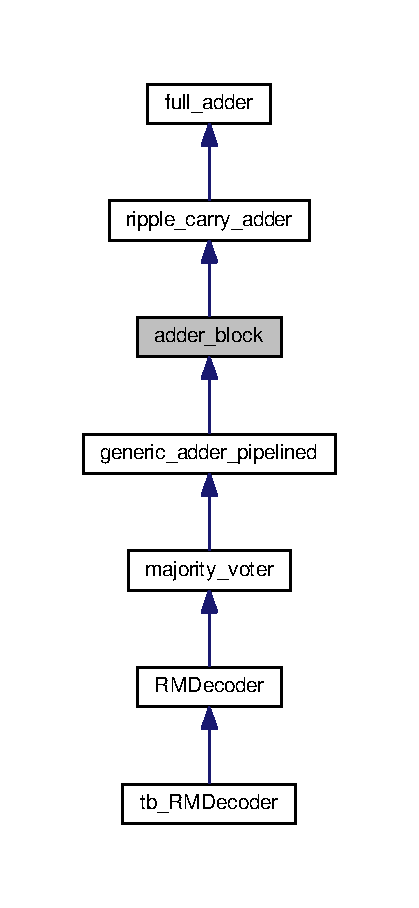
\includegraphics[width=201pt]{classadder__block__inherit__graph}
\end{center}
\end{figure}


Diagramma di collaborazione per adder\+\_\+block\+:\nopagebreak
\begin{figure}[H]
\begin{center}
\leavevmode
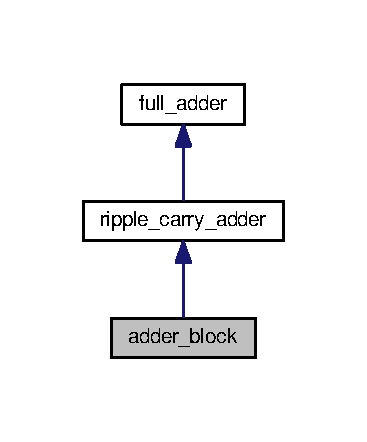
\includegraphics[width=176pt]{classadder__block__coll__graph}
\end{center}
\end{figure}
\subsection*{Entities}
\begin{DoxyCompactItemize}
\item 
\hyperlink{classadder__block_1_1_structural}{Structural} architecture
\end{DoxyCompactItemize}
\subsection*{Libraries}
 \begin{DoxyCompactItemize}
\item 
\hypertarget{classadder__block_gae4f03c286607f3181e16b9aa12d0c6d4}{\hyperlink{group___majority_voter_gae4f03c286607f3181e16b9aa12d0c6d4}{I\+E\+E\+E} }\label{classadder__block_gae4f03c286607f3181e16b9aa12d0c6d4}

\end{DoxyCompactItemize}
\subsection*{Use Clauses}
 \begin{DoxyCompactItemize}
\item 
\hypertarget{classadder__block_gaa4b2b25246a821511120e3149b003563}{\hyperlink{group___majority_voter_gaa4b2b25246a821511120e3149b003563}{S\+T\+D\+\_\+\+L\+O\+G\+I\+C\+\_\+1164}   }\label{classadder__block_gaa4b2b25246a821511120e3149b003563}

\item 
\hypertarget{classadder__block_gae00f3f04545af57582ff10609eee23e2}{\hyperlink{group___majority_voter_gae00f3f04545af57582ff10609eee23e2}{N\+U\+M\+E\+R\+I\+C\+\_\+\+S\+T\+D}   }\label{classadder__block_gae00f3f04545af57582ff10609eee23e2}

\item 
\hypertarget{classadder__block_ga6af860958a1bb510ee63ced87b57e11a}{\hyperlink{group___majority_voter_ga6af860958a1bb510ee63ced87b57e11a}{M\+A\+T\+H\+\_\+\+R\+E\+A\+L}   }\label{classadder__block_ga6af860958a1bb510ee63ced87b57e11a}

\end{DoxyCompactItemize}
\subsection*{Generics}
 \begin{DoxyCompactItemize}
\item 
\hypertarget{classadder__block_gaada2870b1b9b57c2dd2c99528a9d0c9f}{\hyperlink{group___majority_voter_gaada2870b1b9b57c2dd2c99528a9d0c9f}{number\+\_\+operand} {\bfseries {\bfseries \textcolor{vhdlchar}{N\+A\+T\+U\+R\+A\+L}\textcolor{vhdlchar}{ }}}}\label{classadder__block_gaada2870b1b9b57c2dd2c99528a9d0c9f}

\item 
\hypertarget{classadder__block_gaa9b5812094fc3ef126f3d8e4dab5292e}{\hyperlink{group___majority_voter_gaa9b5812094fc3ef126f3d8e4dab5292e}{number\+\_\+bit\+\_\+for\+\_\+operand} {\bfseries {\bfseries \textcolor{vhdlchar}{N\+A\+T\+U\+R\+A\+L}\textcolor{vhdlchar}{ }}}}\label{classadder__block_gaa9b5812094fc3ef126f3d8e4dab5292e}

\item 
\hypertarget{classadder__block_gaf3b6f2fa50cdb3b92a10197ca4e207f9}{\hyperlink{group___majority_voter_gaf3b6f2fa50cdb3b92a10197ca4e207f9}{level} {\bfseries {\bfseries \textcolor{vhdlchar}{N\+A\+T\+U\+R\+A\+L}\textcolor{vhdlchar}{ }}}}\label{classadder__block_gaf3b6f2fa50cdb3b92a10197ca4e207f9}

\end{DoxyCompactItemize}
\subsection*{Ports}
 \begin{DoxyCompactItemize}
\item 
\hypertarget{classadder__block_ga5a138d36775773e82950ee12e1f944de}{\hyperlink{group___majority_voter_ga5a138d36775773e82950ee12e1f944de}{data\+\_\+in}  {\bfseries {\bfseries \textcolor{vhdlchar}{in}\textcolor{vhdlchar}{ }}} {\bfseries \textcolor{vhdlchar}{S\+T\+D\+\_\+\+L\+O\+G\+I\+C\+\_\+\+V\+E\+C\+T\+O\+R}\textcolor{vhdlchar}{ }\textcolor{vhdlchar}{(}\textcolor{vhdlchar}{ }\textcolor{vhdlchar}{ }\textcolor{vhdlchar}{ }\textcolor{vhdlchar}{ }\textcolor{vhdlchar}{number\+\_\+operand}\textcolor{vhdlchar}{$\ast$}\textcolor{vhdlchar}{ }\textcolor{vhdlchar}{ }\textcolor{vhdlchar}{ }\textcolor{vhdlchar}{number\+\_\+bit\+\_\+for\+\_\+operand}\textcolor{vhdlchar}{-\/}\textcolor{vhdlchar}{ } \textcolor{vhdldigit}{1} \textcolor{vhdlchar}{ }\textcolor{vhdlchar}{downto}\textcolor{vhdlchar}{ }\textcolor{vhdlchar}{ } \textcolor{vhdldigit}{0} \textcolor{vhdlchar}{ }\textcolor{vhdlchar}{)}\textcolor{vhdlchar}{ }} }\label{classadder__block_ga5a138d36775773e82950ee12e1f944de}

\item 
\hypertarget{classadder__block_ga55e1fcd272414c24dc7f669e0050e8cc}{\hyperlink{group___majority_voter_ga55e1fcd272414c24dc7f669e0050e8cc}{data\+\_\+out}  {\bfseries {\bfseries \textcolor{vhdlchar}{out}\textcolor{vhdlchar}{ }}} {\bfseries \textcolor{vhdlchar}{S\+T\+D\+\_\+\+L\+O\+G\+I\+C\+\_\+\+V\+E\+C\+T\+O\+R}\textcolor{vhdlchar}{ }\textcolor{vhdlchar}{(}\textcolor{vhdlchar}{ }\textcolor{vhdlchar}{ }\textcolor{vhdlchar}{ }\textcolor{vhdlchar}{ }\textcolor{vhdlchar}{number\+\_\+operand}\textcolor{vhdlchar}{$\ast$}\textcolor{vhdlchar}{ }\textcolor{vhdlchar}{ }\textcolor{vhdlchar}{ }\textcolor{vhdlchar}{number\+\_\+bit\+\_\+for\+\_\+operand}\textcolor{vhdlchar}{-\/}\textcolor{vhdlchar}{ } \textcolor{vhdldigit}{1} \textcolor{vhdlchar}{ }\textcolor{vhdlchar}{downto}\textcolor{vhdlchar}{ }\textcolor{vhdlchar}{ } \textcolor{vhdldigit}{0} \textcolor{vhdlchar}{ }\textcolor{vhdlchar}{)}\textcolor{vhdlchar}{ }} }\label{classadder__block_ga55e1fcd272414c24dc7f669e0050e8cc}

\end{DoxyCompactItemize}


\subsection{Descrizione dettagliata}
Implementazione V\+H\+D\+L \hyperlink{classadder__block_1_1_structural}{Structural} di un generico livello del componente generic\+\_\+adder. Tale livello è costituito da 2$^\wedge$level addizionatori che lavorano in parallelo, di dimensione dipendente dal livello corrente\+: N = number\+\_\+bit\+\_\+for\+\_\+operand + log2(number\+\_\+operand)-\/level-\/1. 


\begin{DoxyParams}{Parametri}
{\em number\+\_\+operand\mbox{[}in\mbox{]}} & parametro che determina il numero di operandi dell' addizionatore \\
\hline
{\em number\+\_\+bit\+\_\+for\+\_\+operand\mbox{[}in\mbox{]}} & parametro che determina il numero di bit di ogni operando \\
\hline
{\em level} & parametro che determina il livello dell'addizionatore che si sta costruendo\\
\hline
{\em data\+\_\+in\mbox{[}in\mbox{]}} & stringa di bit di input di dimensione (number\+\_\+operand $\ast$ number\+\_\+bit\+\_\+for\+\_\+operand) che è la concatenzaione delle somme parziali del livello precedente \\
\hline
{\em data\+\_\+out\mbox{[}out\mbox{]}} & stringa di bit di uscita di dimensione (number\+\_\+operand $\ast$ number\+\_\+bit\+\_\+for\+\_\+operand) che è la concatenzaione delle somme parziali per il livello successivo \\
\hline
\end{DoxyParams}


La documentazione per questa classe è stata generata a partire dal seguente file\+:\begin{DoxyCompactItemize}
\item 
R\+M\+Decoder/\+Majority\+Voter/\hyperlink{adder__block_8vhd}{adder\+\_\+block.\+vhd}\end{DoxyCompactItemize}

\hypertarget{class_generic_buffer_1_1_behavioral}{\section{Behavioral Architecture Reference}
\label{class_generic_buffer_1_1_behavioral}\index{Behavioral@{Behavioral}}
}
\subsection*{Processes}
 \begin{DoxyCompactItemize}
\item 
\hypertarget{class_generic_buffer_1_1_behavioral_ga2ee480e118ca2b3fccf26139a66e84ad}{\hyperlink{group___r_m_decoder_ga2ee480e118ca2b3fccf26139a66e84ad}{P\+R\+O\+C\+E\+S\+S\+\_\+0}{\bfseries  ( {\bfseries \textcolor{vhdlchar}{clock}\textcolor{vhdlchar}{ }} , {\bfseries \textcolor{vhdlchar}{reset\+\_\+n}\textcolor{vhdlchar}{ }} , {\bfseries \textcolor{vhdlchar}{load}\textcolor{vhdlchar}{ }} , {\bfseries \textcolor{vhdlchar}{data\+\_\+in}\textcolor{vhdlchar}{ }} )}}\label{class_generic_buffer_1_1_behavioral_ga2ee480e118ca2b3fccf26139a66e84ad}

\end{DoxyCompactItemize}
\subsection*{Signals}
 \begin{DoxyCompactItemize}
\item 
\hypertarget{class_generic_buffer_1_1_behavioral_gab94e66105790803865249c33633e359f}{\hyperlink{group___r_m_decoder_gab94e66105790803865249c33633e359f}{tmp} {\bfseries \textcolor{vhdlchar}{std\+\_\+logic\+\_\+vector}\textcolor{vhdlchar}{ }\textcolor{vhdlchar}{(}\textcolor{vhdlchar}{ }\textcolor{vhdlchar}{ }\textcolor{vhdlchar}{ }\textcolor{vhdlchar}{ }\textcolor{vhdlchar}{width}\textcolor{vhdlchar}{-\/}\textcolor{vhdlchar}{ } \textcolor{vhdldigit}{1} \textcolor{vhdlchar}{ }\textcolor{vhdlchar}{downto}\textcolor{vhdlchar}{ }\textcolor{vhdlchar}{ } \textcolor{vhdldigit}{0} \textcolor{vhdlchar}{ }\textcolor{vhdlchar}{)}\textcolor{vhdlchar}{ }\textcolor{vhdlchar}{ }\textcolor{vhdlchar}{ }\textcolor{vhdlchar}{\+:}\textcolor{vhdlchar}{=}\textcolor{vhdlchar}{ }\textcolor{vhdlchar}{(}\textcolor{vhdlchar}{ }\textcolor{vhdlchar}{ }\textcolor{vhdlchar}{others}\textcolor{vhdlchar}{ }\textcolor{vhdlchar}{ }\textcolor{vhdlchar}{=}\textcolor{vhdlchar}{ }\textcolor{vhdlchar}{$>$}\textcolor{vhdlchar}{ }\textcolor{vhdlchar}{'}\textcolor{vhdlchar}{ } \textcolor{vhdldigit}{0} \textcolor{vhdlchar}{ }\textcolor{vhdlchar}{'}\textcolor{vhdlchar}{ }\textcolor{vhdlchar}{)}\textcolor{vhdlchar}{ }} }\label{class_generic_buffer_1_1_behavioral_gab94e66105790803865249c33633e359f}

\end{DoxyCompactItemize}


La documentazione per questa classe è stata generata a partire dal seguente file\+:\begin{DoxyCompactItemize}
\item 
R\+M\+Decoder/Generic\+Buffer.\+vhd\end{DoxyCompactItemize}

\hypertarget{classtb___r_m_decoder_1_1_behavioral}{\section{Behavioral Architecture Reference}
\label{classtb___r_m_decoder_1_1_behavioral}\index{Behavioral@{Behavioral}}
}
\subsection*{Processes}
 \begin{DoxyCompactItemize}
\item 
\hypertarget{classtb___r_m_decoder_1_1_behavioral_ac0731c1f0a226305f2a590b4044cdccb}{\hyperlink{classtb___r_m_decoder_1_1_behavioral_ac0731c1f0a226305f2a590b4044cdccb}{clock\+\_\+process}{\bfseries  (  )}}\label{classtb___r_m_decoder_1_1_behavioral_ac0731c1f0a226305f2a590b4044cdccb}

\item 
\hypertarget{classtb___r_m_decoder_1_1_behavioral_gaee7e8b077315d73d2c245522dd7ba9a8}{\hyperlink{group___r_m_decoder_gaee7e8b077315d73d2c245522dd7ba9a8}{stim\+\_\+process}{\bfseries  (  )}}\label{classtb___r_m_decoder_1_1_behavioral_gaee7e8b077315d73d2c245522dd7ba9a8}

\end{DoxyCompactItemize}
\subsection*{Components}
 \begin{DoxyCompactItemize}
\item 
\hypertarget{classtb___r_m_decoder_1_1_behavioral_gaa428b5ac9b6611fe96abf435a343d47c}{\hyperlink{group___r_m_decoder_gaa428b5ac9b6611fe96abf435a343d47c}{R\+M\+Decoder}  {\bfseries }  }\label{classtb___r_m_decoder_1_1_behavioral_gaa428b5ac9b6611fe96abf435a343d47c}

\end{DoxyCompactItemize}
\subsection*{Constants}
 \begin{DoxyCompactItemize}
\item 
\hypertarget{classtb___r_m_decoder_1_1_behavioral_ga66500af96850e5a149ace8e4005a489a}{\hyperlink{group___r_m_decoder_ga66500af96850e5a149ace8e4005a489a}{m} {\bfseries \textcolor{comment}{natural}\textcolor{vhdlchar}{ }\textcolor{vhdlchar}{ }\textcolor{vhdlchar}{\+:}\textcolor{vhdlchar}{=}\textcolor{vhdlchar}{ }\textcolor{vhdlchar}{ } \textcolor{vhdldigit}{4} \textcolor{vhdlchar}{ }} }\label{classtb___r_m_decoder_1_1_behavioral_ga66500af96850e5a149ace8e4005a489a}

\item 
\hypertarget{classtb___r_m_decoder_1_1_behavioral_ga9fb080b7379b7a2f64508f2e5c5f0cba}{\hyperlink{group___r_m_decoder_ga9fb080b7379b7a2f64508f2e5c5f0cba}{encoded} {\bfseries \textcolor{vhdlchar}{matrix}\textcolor{vhdlchar}{ }\textcolor{vhdlchar}{(}\textcolor{vhdlchar}{ }\textcolor{vhdlchar}{ } \textcolor{vhdldigit}{0} \textcolor{vhdlchar}{ }\textcolor{keywordflow}{to}\textcolor{vhdlchar}{ }\textcolor{vhdlchar}{ } \textcolor{vhdldigit}{2} \textcolor{vhdlchar}{$\ast$}\textcolor{vhdlchar}{$\ast$}\textcolor{vhdlchar}{ }\textcolor{vhdlchar}{(}\textcolor{vhdlchar}{ }\textcolor{vhdlchar}{ }\textcolor{vhdlchar}{ }\textcolor{vhdlchar}{ }\textcolor{vhdlchar}{m}\textcolor{vhdlchar}{+}\textcolor{vhdlchar}{ } \textcolor{vhdldigit}{1} \textcolor{vhdlchar}{ }\textcolor{vhdlchar}{)}\textcolor{vhdlchar}{ }\textcolor{vhdlchar}{-\/}\textcolor{vhdlchar}{ } \textcolor{vhdldigit}{1} \textcolor{vhdlchar}{ }\textcolor{vhdlchar}{)}\textcolor{vhdlchar}{ }\textcolor{vhdlchar}{ }\textcolor{vhdlchar}{ }\textcolor{vhdlchar}{\+:}\textcolor{vhdlchar}{=}\textcolor{vhdlchar}{ }\textcolor{vhdlchar}{(}\textcolor{vhdlchar}{ }\textcolor{vhdlchar}{(}\textcolor{vhdlchar}{ }\textcolor{vhdlchar}{ }\textcolor{vhdlchar}{x}\textcolor{vhdlchar}{ }\textcolor{keyword}{\char`\"{} 0000 \char`\"{}}\textcolor{vhdlchar}{ }\textcolor{vhdlchar}{)}\textcolor{vhdlchar}{ }\textcolor{vhdlchar}{,}\textcolor{vhdlchar}{ }\textcolor{vhdlchar}{(}\textcolor{vhdlchar}{ }\textcolor{vhdlchar}{ }\textcolor{vhdlchar}{x}\textcolor{vhdlchar}{ }\textcolor{keyword}{\char`\"{} 5555 \char`\"{}}\textcolor{vhdlchar}{ }\textcolor{vhdlchar}{)}\textcolor{vhdlchar}{ }\textcolor{vhdlchar}{,}\textcolor{vhdlchar}{ }\textcolor{vhdlchar}{(}\textcolor{vhdlchar}{ }\textcolor{vhdlchar}{ }\textcolor{vhdlchar}{x}\textcolor{vhdlchar}{ }\textcolor{keyword}{\char`\"{} 3333 \char`\"{}}\textcolor{vhdlchar}{ }\textcolor{vhdlchar}{)}\textcolor{vhdlchar}{ }\textcolor{vhdlchar}{,}\textcolor{vhdlchar}{ }\textcolor{vhdlchar}{(}\textcolor{vhdlchar}{ }\textcolor{vhdlchar}{ }\textcolor{vhdlchar}{x}\textcolor{vhdlchar}{ }\textcolor{keyword}{\char`\"{} 6666 \char`\"{}}\textcolor{vhdlchar}{ }\textcolor{vhdlchar}{)}\textcolor{vhdlchar}{ }\textcolor{vhdlchar}{,}\textcolor{vhdlchar}{ }\textcolor{vhdlchar}{(}\textcolor{vhdlchar}{ }\textcolor{vhdlchar}{ }\textcolor{vhdlchar}{x}\textcolor{vhdlchar}{ }\textcolor{keyword}{\char`\"{} 0f0f \char`\"{}}\textcolor{vhdlchar}{ }\textcolor{vhdlchar}{)}\textcolor{vhdlchar}{ }\textcolor{vhdlchar}{,}\textcolor{vhdlchar}{ }\textcolor{vhdlchar}{(}\textcolor{vhdlchar}{ }\textcolor{vhdlchar}{ }\textcolor{vhdlchar}{x}\textcolor{vhdlchar}{ }\textcolor{keyword}{\char`\"{} 5a5a \char`\"{}}\textcolor{vhdlchar}{ }\textcolor{vhdlchar}{)}\textcolor{vhdlchar}{ }\textcolor{vhdlchar}{,}\textcolor{vhdlchar}{ }\textcolor{vhdlchar}{(}\textcolor{vhdlchar}{ }\textcolor{vhdlchar}{ }\textcolor{vhdlchar}{x}\textcolor{vhdlchar}{ }\textcolor{keyword}{\char`\"{} 3c3c \char`\"{}}\textcolor{vhdlchar}{ }\textcolor{vhdlchar}{)}\textcolor{vhdlchar}{ }\textcolor{vhdlchar}{,}\textcolor{vhdlchar}{ }\textcolor{vhdlchar}{(}\textcolor{vhdlchar}{ }\textcolor{vhdlchar}{ }\textcolor{vhdlchar}{x}\textcolor{vhdlchar}{ }\textcolor{keyword}{\char`\"{} 6969 \char`\"{}}\textcolor{vhdlchar}{ }\textcolor{vhdlchar}{)}\textcolor{vhdlchar}{ }\textcolor{vhdlchar}{,}\textcolor{vhdlchar}{ }\textcolor{vhdlchar}{(}\textcolor{vhdlchar}{ }\textcolor{vhdlchar}{ }\textcolor{vhdlchar}{x}\textcolor{vhdlchar}{ }\textcolor{keyword}{\char`\"{} 00ff \char`\"{}}\textcolor{vhdlchar}{ }\textcolor{vhdlchar}{)}\textcolor{vhdlchar}{ }\textcolor{vhdlchar}{,}\textcolor{vhdlchar}{ }\textcolor{vhdlchar}{(}\textcolor{vhdlchar}{ }\textcolor{vhdlchar}{ }\textcolor{vhdlchar}{x}\textcolor{vhdlchar}{ }\textcolor{keyword}{\char`\"{} 55aa \char`\"{}}\textcolor{vhdlchar}{ }\textcolor{vhdlchar}{)}\textcolor{vhdlchar}{ }\textcolor{vhdlchar}{,}\textcolor{vhdlchar}{ }\textcolor{vhdlchar}{(}\textcolor{vhdlchar}{ }\textcolor{vhdlchar}{ }\textcolor{vhdlchar}{x}\textcolor{vhdlchar}{ }\textcolor{keyword}{\char`\"{} 33cc \char`\"{}}\textcolor{vhdlchar}{ }\textcolor{vhdlchar}{)}\textcolor{vhdlchar}{ }\textcolor{vhdlchar}{,}\textcolor{vhdlchar}{ }\textcolor{vhdlchar}{(}\textcolor{vhdlchar}{ }\textcolor{vhdlchar}{ }\textcolor{vhdlchar}{x}\textcolor{vhdlchar}{ }\textcolor{keyword}{\char`\"{} 6699 \char`\"{}}\textcolor{vhdlchar}{ }\textcolor{vhdlchar}{)}\textcolor{vhdlchar}{ }\textcolor{vhdlchar}{,}\textcolor{vhdlchar}{ }\textcolor{vhdlchar}{(}\textcolor{vhdlchar}{ }\textcolor{vhdlchar}{ }\textcolor{vhdlchar}{x}\textcolor{vhdlchar}{ }\textcolor{keyword}{\char`\"{} 0ff0 \char`\"{}}\textcolor{vhdlchar}{ }\textcolor{vhdlchar}{)}\textcolor{vhdlchar}{ }\textcolor{vhdlchar}{,}\textcolor{vhdlchar}{ }\textcolor{vhdlchar}{(}\textcolor{vhdlchar}{ }\textcolor{vhdlchar}{ }\textcolor{vhdlchar}{x}\textcolor{vhdlchar}{ }\textcolor{keyword}{\char`\"{} 5aa5 \char`\"{}}\textcolor{vhdlchar}{ }\textcolor{vhdlchar}{)}\textcolor{vhdlchar}{ }\textcolor{vhdlchar}{,}\textcolor{vhdlchar}{ }\textcolor{vhdlchar}{(}\textcolor{vhdlchar}{ }\textcolor{vhdlchar}{ }\textcolor{vhdlchar}{x}\textcolor{vhdlchar}{ }\textcolor{keyword}{\char`\"{} 3cc3 \char`\"{}}\textcolor{vhdlchar}{ }\textcolor{vhdlchar}{)}\textcolor{vhdlchar}{ }\textcolor{vhdlchar}{,}\textcolor{vhdlchar}{ }\textcolor{vhdlchar}{(}\textcolor{vhdlchar}{ }\textcolor{vhdlchar}{ }\textcolor{vhdlchar}{x}\textcolor{vhdlchar}{ }\textcolor{keyword}{\char`\"{} 6996 \char`\"{}}\textcolor{vhdlchar}{ }\textcolor{vhdlchar}{)}\textcolor{vhdlchar}{ }\textcolor{vhdlchar}{,}\textcolor{vhdlchar}{ }\textcolor{vhdlchar}{(}\textcolor{vhdlchar}{ }\textcolor{vhdlchar}{ }\textcolor{vhdlchar}{x}\textcolor{vhdlchar}{ }\textcolor{keyword}{\char`\"{} ffff \char`\"{}}\textcolor{vhdlchar}{ }\textcolor{vhdlchar}{)}\textcolor{vhdlchar}{ }\textcolor{vhdlchar}{,}\textcolor{vhdlchar}{ }\textcolor{vhdlchar}{(}\textcolor{vhdlchar}{ }\textcolor{vhdlchar}{ }\textcolor{vhdlchar}{x}\textcolor{vhdlchar}{ }\textcolor{keyword}{\char`\"{} aaaa \char`\"{}}\textcolor{vhdlchar}{ }\textcolor{vhdlchar}{)}\textcolor{vhdlchar}{ }\textcolor{vhdlchar}{,}\textcolor{vhdlchar}{ }\textcolor{vhdlchar}{(}\textcolor{vhdlchar}{ }\textcolor{vhdlchar}{ }\textcolor{vhdlchar}{x}\textcolor{vhdlchar}{ }\textcolor{keyword}{\char`\"{} cccc \char`\"{}}\textcolor{vhdlchar}{ }\textcolor{vhdlchar}{)}\textcolor{vhdlchar}{ }\textcolor{vhdlchar}{,}\textcolor{vhdlchar}{ }\textcolor{vhdlchar}{(}\textcolor{vhdlchar}{ }\textcolor{vhdlchar}{ }\textcolor{vhdlchar}{x}\textcolor{vhdlchar}{ }\textcolor{keyword}{\char`\"{} 9999 \char`\"{}}\textcolor{vhdlchar}{ }\textcolor{vhdlchar}{)}\textcolor{vhdlchar}{ }\textcolor{vhdlchar}{,}\textcolor{vhdlchar}{ }\textcolor{vhdlchar}{(}\textcolor{vhdlchar}{ }\textcolor{vhdlchar}{ }\textcolor{vhdlchar}{x}\textcolor{vhdlchar}{ }\textcolor{keyword}{\char`\"{} f0f0 \char`\"{}}\textcolor{vhdlchar}{ }\textcolor{vhdlchar}{)}\textcolor{vhdlchar}{ }\textcolor{vhdlchar}{,}\textcolor{vhdlchar}{ }\textcolor{vhdlchar}{(}\textcolor{vhdlchar}{ }\textcolor{vhdlchar}{ }\textcolor{vhdlchar}{x}\textcolor{vhdlchar}{ }\textcolor{keyword}{\char`\"{} a5a5 \char`\"{}}\textcolor{vhdlchar}{ }\textcolor{vhdlchar}{)}\textcolor{vhdlchar}{ }\textcolor{vhdlchar}{,}\textcolor{vhdlchar}{ }\textcolor{vhdlchar}{(}\textcolor{vhdlchar}{ }\textcolor{vhdlchar}{ }\textcolor{vhdlchar}{x}\textcolor{vhdlchar}{ }\textcolor{keyword}{\char`\"{} c3c3 \char`\"{}}\textcolor{vhdlchar}{ }\textcolor{vhdlchar}{)}\textcolor{vhdlchar}{ }\textcolor{vhdlchar}{,}\textcolor{vhdlchar}{ }\textcolor{vhdlchar}{(}\textcolor{vhdlchar}{ }\textcolor{vhdlchar}{ }\textcolor{vhdlchar}{x}\textcolor{vhdlchar}{ }\textcolor{keyword}{\char`\"{} 9696 \char`\"{}}\textcolor{vhdlchar}{ }\textcolor{vhdlchar}{)}\textcolor{vhdlchar}{ }\textcolor{vhdlchar}{,}\textcolor{vhdlchar}{ }\textcolor{vhdlchar}{(}\textcolor{vhdlchar}{ }\textcolor{vhdlchar}{ }\textcolor{vhdlchar}{x}\textcolor{vhdlchar}{ }\textcolor{keyword}{\char`\"{} ff00 \char`\"{}}\textcolor{vhdlchar}{ }\textcolor{vhdlchar}{)}\textcolor{vhdlchar}{ }\textcolor{vhdlchar}{,}\textcolor{vhdlchar}{ }\textcolor{vhdlchar}{(}\textcolor{vhdlchar}{ }\textcolor{vhdlchar}{ }\textcolor{vhdlchar}{x}\textcolor{vhdlchar}{ }\textcolor{keyword}{\char`\"{} aa55 \char`\"{}}\textcolor{vhdlchar}{ }\textcolor{vhdlchar}{)}\textcolor{vhdlchar}{ }\textcolor{vhdlchar}{,}\textcolor{vhdlchar}{ }\textcolor{vhdlchar}{(}\textcolor{vhdlchar}{ }\textcolor{vhdlchar}{ }\textcolor{vhdlchar}{x}\textcolor{vhdlchar}{ }\textcolor{keyword}{\char`\"{} cc33 \char`\"{}}\textcolor{vhdlchar}{ }\textcolor{vhdlchar}{)}\textcolor{vhdlchar}{ }\textcolor{vhdlchar}{,}\textcolor{vhdlchar}{ }\textcolor{vhdlchar}{(}\textcolor{vhdlchar}{ }\textcolor{vhdlchar}{ }\textcolor{vhdlchar}{x}\textcolor{vhdlchar}{ }\textcolor{keyword}{\char`\"{} 9966 \char`\"{}}\textcolor{vhdlchar}{ }\textcolor{vhdlchar}{)}\textcolor{vhdlchar}{ }\textcolor{vhdlchar}{,}\textcolor{vhdlchar}{ }\textcolor{vhdlchar}{(}\textcolor{vhdlchar}{ }\textcolor{vhdlchar}{ }\textcolor{vhdlchar}{x}\textcolor{vhdlchar}{ }\textcolor{keyword}{\char`\"{} f00f \char`\"{}}\textcolor{vhdlchar}{ }\textcolor{vhdlchar}{)}\textcolor{vhdlchar}{ }\textcolor{vhdlchar}{,}\textcolor{vhdlchar}{ }\textcolor{vhdlchar}{(}\textcolor{vhdlchar}{ }\textcolor{vhdlchar}{ }\textcolor{vhdlchar}{x}\textcolor{vhdlchar}{ }\textcolor{keyword}{\char`\"{} a55a \char`\"{}}\textcolor{vhdlchar}{ }\textcolor{vhdlchar}{)}\textcolor{vhdlchar}{ }\textcolor{vhdlchar}{,}\textcolor{vhdlchar}{ }\textcolor{vhdlchar}{(}\textcolor{vhdlchar}{ }\textcolor{vhdlchar}{ }\textcolor{vhdlchar}{x}\textcolor{vhdlchar}{ }\textcolor{keyword}{\char`\"{} c33c \char`\"{}}\textcolor{vhdlchar}{ }\textcolor{vhdlchar}{)}\textcolor{vhdlchar}{ }\textcolor{vhdlchar}{,}\textcolor{vhdlchar}{ }\textcolor{vhdlchar}{(}\textcolor{vhdlchar}{ }\textcolor{vhdlchar}{ }\textcolor{vhdlchar}{x}\textcolor{vhdlchar}{ }\textcolor{keyword}{\char`\"{} 9669 \char`\"{}}\textcolor{vhdlchar}{ }\textcolor{vhdlchar}{)}\textcolor{vhdlchar}{ }} }\label{classtb___r_m_decoder_1_1_behavioral_ga9fb080b7379b7a2f64508f2e5c5f0cba}

\item 
\hypertarget{classtb___r_m_decoder_1_1_behavioral_ga56b871d5221ff49e502a0ac86ad875ea}{\hyperlink{group___r_m_decoder_ga56b871d5221ff49e502a0ac86ad875ea}{clock\+\_\+period} {\bfseries \textcolor{comment}{time}\textcolor{vhdlchar}{ }\textcolor{vhdlchar}{ }\textcolor{vhdlchar}{\+:}\textcolor{vhdlchar}{=}\textcolor{vhdlchar}{ }\textcolor{vhdlchar}{ }\textcolor{vhdlchar}{ } \textcolor{vhdldigit}{10} \textcolor{vhdlchar}{ }\textcolor{vhdlchar}{ns}\textcolor{vhdlchar}{ }} }\label{classtb___r_m_decoder_1_1_behavioral_ga56b871d5221ff49e502a0ac86ad875ea}

\item 
\hypertarget{classtb___r_m_decoder_1_1_behavioral_ga57b43bd889cdfa2bf9597490517dd675}{\hyperlink{group___r_m_decoder_ga57b43bd889cdfa2bf9597490517dd675}{generator\+\_\+matrix\+\_\+01} {\bfseries \textcolor{comment}{boolean}\textcolor{vhdlchar}{ }\textcolor{vhdlchar}{ }\textcolor{vhdlchar}{\+:}\textcolor{vhdlchar}{=}\textcolor{vhdlchar}{ }\textcolor{vhdlchar}{ }\textcolor{vhdlchar}{ }\textcolor{vhdlchar}{ }\textcolor{vhdlchar}{true}\textcolor{vhdlchar}{ }} }\label{classtb___r_m_decoder_1_1_behavioral_ga57b43bd889cdfa2bf9597490517dd675}

\end{DoxyCompactItemize}
\subsection*{Types}
 \begin{DoxyCompactItemize}
\item 
\hypertarget{classtb___r_m_decoder_1_1_behavioral_ga016dcfd62eba82b89adb229b316a92ce}{{\bfseries \hyperlink{group___r_m_decoder_ga016dcfd62eba82b89adb229b316a92ce}{matrix}{\bfseries \textcolor{keywordflow}{array}\textcolor{vhdlchar}{ }\textcolor{vhdlchar}{(}\textcolor{vhdlchar}{ }\textcolor{comment}{natural}\textcolor{vhdlchar}{ }\textcolor{keywordflow}{range}\textcolor{vhdlchar}{ }\textcolor{vhdlchar}{$<$$>$}\textcolor{vhdlchar}{ }\textcolor{vhdlchar}{)}\textcolor{vhdlchar}{ }\textcolor{vhdlchar}{ }\textcolor{keywordflow}{of}\textcolor{vhdlchar}{ }\textcolor{comment}{std\+\_\+logic\+\_\+vector}\textcolor{vhdlchar}{ }\textcolor{vhdlchar}{(}\textcolor{vhdlchar}{ }\textcolor{vhdlchar}{ } \textcolor{vhdldigit}{2} \textcolor{vhdlchar}{$\ast$}\textcolor{vhdlchar}{$\ast$}\textcolor{vhdlchar}{ }\textcolor{vhdlchar}{ }\textcolor{vhdlchar}{ }\textcolor{vhdlchar}{m}\textcolor{vhdlchar}{-\/}\textcolor{vhdlchar}{ } \textcolor{vhdldigit}{1} \textcolor{vhdlchar}{ }\textcolor{keywordflow}{downto}\textcolor{vhdlchar}{ }\textcolor{vhdlchar}{ } \textcolor{vhdldigit}{0} \textcolor{vhdlchar}{ }\textcolor{vhdlchar}{)}\textcolor{vhdlchar}{ }}} }\label{classtb___r_m_decoder_1_1_behavioral_ga016dcfd62eba82b89adb229b316a92ce}

\end{DoxyCompactItemize}
\subsection*{Signals}
 \begin{DoxyCompactItemize}
\item 
\hypertarget{classtb___r_m_decoder_1_1_behavioral_ga88534be3ae2cd34bca41082dac12aad4}{\hyperlink{group___r_m_decoder_ga88534be3ae2cd34bca41082dac12aad4}{clock} {\bfseries \textcolor{comment}{std\+\_\+logic}\textcolor{vhdlchar}{ }\textcolor{vhdlchar}{ }\textcolor{vhdlchar}{\+:}\textcolor{vhdlchar}{=}\textcolor{vhdlchar}{ }\textcolor{vhdlchar}{ }\textcolor{vhdlchar}{'}\textcolor{vhdlchar}{ } \textcolor{vhdldigit}{0} \textcolor{vhdlchar}{ }\textcolor{vhdlchar}{'}\textcolor{vhdlchar}{ }} }\label{classtb___r_m_decoder_1_1_behavioral_ga88534be3ae2cd34bca41082dac12aad4}

\item 
\hypertarget{classtb___r_m_decoder_1_1_behavioral_gaa4a138c19128c1545acb81fdfa2664f4}{\hyperlink{group___r_m_decoder_gaa4a138c19128c1545acb81fdfa2664f4}{reset\+\_\+n} {\bfseries \textcolor{comment}{std\+\_\+logic}\textcolor{vhdlchar}{ }\textcolor{vhdlchar}{ }\textcolor{vhdlchar}{\+:}\textcolor{vhdlchar}{=}\textcolor{vhdlchar}{ }\textcolor{vhdlchar}{ }\textcolor{vhdlchar}{'}\textcolor{vhdlchar}{ } \textcolor{vhdldigit}{0} \textcolor{vhdlchar}{ }\textcolor{vhdlchar}{'}\textcolor{vhdlchar}{ }} }\label{classtb___r_m_decoder_1_1_behavioral_gaa4a138c19128c1545acb81fdfa2664f4}

\item 
\hypertarget{classtb___r_m_decoder_1_1_behavioral_gadefa2781585771b2e103759ab207c9c9}{\hyperlink{group___r_m_decoder_gadefa2781585771b2e103759ab207c9c9}{data\+\_\+in} {\bfseries \textcolor{comment}{std\+\_\+logic\+\_\+vector}\textcolor{vhdlchar}{ }\textcolor{vhdlchar}{(}\textcolor{vhdlchar}{ }\textcolor{vhdlchar}{ } \textcolor{vhdldigit}{2} \textcolor{vhdlchar}{$\ast$}\textcolor{vhdlchar}{$\ast$}\textcolor{vhdlchar}{ }\textcolor{vhdlchar}{ }\textcolor{vhdlchar}{ }\textcolor{vhdlchar}{m}\textcolor{vhdlchar}{-\/}\textcolor{vhdlchar}{ } \textcolor{vhdldigit}{1} \textcolor{vhdlchar}{ }\textcolor{keywordflow}{downto}\textcolor{vhdlchar}{ }\textcolor{vhdlchar}{ } \textcolor{vhdldigit}{0} \textcolor{vhdlchar}{ }\textcolor{vhdlchar}{)}\textcolor{vhdlchar}{ }\textcolor{vhdlchar}{ }\textcolor{vhdlchar}{ }\textcolor{vhdlchar}{\+:}\textcolor{vhdlchar}{=}\textcolor{vhdlchar}{ }\textcolor{vhdlchar}{(}\textcolor{vhdlchar}{ }\textcolor{vhdlchar}{ }\textcolor{keywordflow}{others}\textcolor{vhdlchar}{ }\textcolor{vhdlchar}{ }\textcolor{vhdlchar}{=}\textcolor{vhdlchar}{ }\textcolor{vhdlchar}{$>$}\textcolor{vhdlchar}{ }\textcolor{vhdlchar}{'}\textcolor{vhdlchar}{ } \textcolor{vhdldigit}{0} \textcolor{vhdlchar}{ }\textcolor{vhdlchar}{'}\textcolor{vhdlchar}{ }\textcolor{vhdlchar}{)}\textcolor{vhdlchar}{ }} }\label{classtb___r_m_decoder_1_1_behavioral_gadefa2781585771b2e103759ab207c9c9}

\item 
\hypertarget{classtb___r_m_decoder_1_1_behavioral_ga0bdb7fe05ee2f31a8225c058816320c7}{\hyperlink{group___r_m_decoder_ga0bdb7fe05ee2f31a8225c058816320c7}{data\+\_\+out} {\bfseries \textcolor{comment}{std\+\_\+logic\+\_\+vector}\textcolor{vhdlchar}{ }\textcolor{vhdlchar}{(}\textcolor{vhdlchar}{ }\textcolor{vhdlchar}{ }\textcolor{vhdlchar}{ }\textcolor{vhdlchar}{ }\textcolor{vhdlchar}{m}\textcolor{vhdlchar}{ }\textcolor{keywordflow}{downto}\textcolor{vhdlchar}{ }\textcolor{vhdlchar}{ } \textcolor{vhdldigit}{0} \textcolor{vhdlchar}{ }\textcolor{vhdlchar}{)}\textcolor{vhdlchar}{ }\textcolor{vhdlchar}{ }\textcolor{vhdlchar}{ }\textcolor{vhdlchar}{\+:}\textcolor{vhdlchar}{=}\textcolor{vhdlchar}{ }\textcolor{vhdlchar}{(}\textcolor{vhdlchar}{ }\textcolor{vhdlchar}{ }\textcolor{keywordflow}{others}\textcolor{vhdlchar}{ }\textcolor{vhdlchar}{ }\textcolor{vhdlchar}{=}\textcolor{vhdlchar}{ }\textcolor{vhdlchar}{$>$}\textcolor{vhdlchar}{ }\textcolor{vhdlchar}{'}\textcolor{vhdlchar}{ } \textcolor{vhdldigit}{0} \textcolor{vhdlchar}{ }\textcolor{vhdlchar}{'}\textcolor{vhdlchar}{ }\textcolor{vhdlchar}{)}\textcolor{vhdlchar}{ }} }\label{classtb___r_m_decoder_1_1_behavioral_ga0bdb7fe05ee2f31a8225c058816320c7}

\end{DoxyCompactItemize}
\subsection*{Instantiations}
 \begin{DoxyCompactItemize}
\item 
\hypertarget{classtb___r_m_decoder_1_1_behavioral_a1619316ad715601eb5d3559db829ac05}{\hyperlink{classtb___r_m_decoder_1_1_behavioral_a1619316ad715601eb5d3559db829ac05}{uut}  {\bfseries R\+M\+Decoder}   }\label{classtb___r_m_decoder_1_1_behavioral_a1619316ad715601eb5d3559db829ac05}

\end{DoxyCompactItemize}


La documentazione per questa classe è stata generata a partire dal seguente file\+:\begin{DoxyCompactItemize}
\item 
R\+M\+Decoder/tb\+\_\+\+R\+M\+Decoder.\+vhd\end{DoxyCompactItemize}

\hypertarget{classtb___r_m_encoder_1_1_behavioral}{\section{Behavioral Architecture Reference}
\label{classtb___r_m_encoder_1_1_behavioral}\index{Behavioral@{Behavioral}}
}
\subsection*{Processes}
 \begin{DoxyCompactItemize}
\item 
\hypertarget{classtb___r_m_encoder_1_1_behavioral_aee7e8b077315d73d2c245522dd7ba9a8}{\hyperlink{classtb___r_m_encoder_1_1_behavioral_aee7e8b077315d73d2c245522dd7ba9a8}{stim\+\_\+process}{\bfseries  (  )}}\label{classtb___r_m_encoder_1_1_behavioral_aee7e8b077315d73d2c245522dd7ba9a8}

\end{DoxyCompactItemize}
\subsection*{Components}
 \begin{DoxyCompactItemize}
\item 
\hypertarget{classtb___r_m_encoder_1_1_behavioral_ga338c5c28a63318ccdef8b2636aaddbc2}{\hyperlink{group___r_m_encoder_ga338c5c28a63318ccdef8b2636aaddbc2}{R\+M\+Encoder}  {\bfseries }  }\label{classtb___r_m_encoder_1_1_behavioral_ga338c5c28a63318ccdef8b2636aaddbc2}

\end{DoxyCompactItemize}
\subsection*{Constants}
 \begin{DoxyCompactItemize}
\item 
\hypertarget{classtb___r_m_encoder_1_1_behavioral_gae28cb25876e016138a9c4bd9ec290160}{\hyperlink{group___r_m_encoder_gae28cb25876e016138a9c4bd9ec290160}{period} {\bfseries \textcolor{comment}{time}\textcolor{vhdlchar}{ }\textcolor{vhdlchar}{ }\textcolor{vhdlchar}{\+:}\textcolor{vhdlchar}{=}\textcolor{vhdlchar}{ }\textcolor{vhdlchar}{ }\textcolor{vhdlchar}{ } \textcolor{vhdldigit}{10} \textcolor{vhdlchar}{ }\textcolor{vhdlchar}{ns}\textcolor{vhdlchar}{ }} }\label{classtb___r_m_encoder_1_1_behavioral_gae28cb25876e016138a9c4bd9ec290160}

\item 
\hypertarget{classtb___r_m_encoder_1_1_behavioral_ga66500af96850e5a149ace8e4005a489a}{\hyperlink{group___r_m_encoder_ga66500af96850e5a149ace8e4005a489a}{m} {\bfseries \textcolor{comment}{natural}\textcolor{vhdlchar}{ }\textcolor{vhdlchar}{ }\textcolor{vhdlchar}{\+:}\textcolor{vhdlchar}{=}\textcolor{vhdlchar}{ }\textcolor{vhdlchar}{ } \textcolor{vhdldigit}{4} \textcolor{vhdlchar}{ }} }\label{classtb___r_m_encoder_1_1_behavioral_ga66500af96850e5a149ace8e4005a489a}

\item 
\hypertarget{classtb___r_m_encoder_1_1_behavioral_ga57b43bd889cdfa2bf9597490517dd675}{\hyperlink{group___r_m_encoder_ga57b43bd889cdfa2bf9597490517dd675}{generator\+\_\+matrix\+\_\+01} {\bfseries \textcolor{comment}{boolean}\textcolor{vhdlchar}{ }\textcolor{vhdlchar}{ }\textcolor{vhdlchar}{\+:}\textcolor{vhdlchar}{=}\textcolor{vhdlchar}{ }\textcolor{vhdlchar}{ }\textcolor{vhdlchar}{ }\textcolor{vhdlchar}{ }\textcolor{vhdlchar}{true}\textcolor{vhdlchar}{ }} }\label{classtb___r_m_encoder_1_1_behavioral_ga57b43bd889cdfa2bf9597490517dd675}

\end{DoxyCompactItemize}
\subsection*{Signals}
 \begin{DoxyCompactItemize}
\item 
\hypertarget{classtb___r_m_encoder_1_1_behavioral_ga88534be3ae2cd34bca41082dac12aad4}{\hyperlink{group___r_m_encoder_ga88534be3ae2cd34bca41082dac12aad4}{clock} {\bfseries \textcolor{comment}{std\+\_\+logic}\textcolor{vhdlchar}{ }\textcolor{vhdlchar}{ }\textcolor{vhdlchar}{\+:}\textcolor{vhdlchar}{=}\textcolor{vhdlchar}{ }\textcolor{vhdlchar}{ }\textcolor{vhdlchar}{'}\textcolor{vhdlchar}{ } \textcolor{vhdldigit}{0} \textcolor{vhdlchar}{ }\textcolor{vhdlchar}{'}\textcolor{vhdlchar}{ }} }\label{classtb___r_m_encoder_1_1_behavioral_ga88534be3ae2cd34bca41082dac12aad4}

\item 
\hypertarget{classtb___r_m_encoder_1_1_behavioral_ga9c2b073d8b653dee5532948bb4b0612a}{\hyperlink{group___r_m_encoder_ga9c2b073d8b653dee5532948bb4b0612a}{data\+\_\+in} {\bfseries \textcolor{comment}{std\+\_\+logic\+\_\+vector}\textcolor{vhdlchar}{ }\textcolor{vhdlchar}{(}\textcolor{vhdlchar}{ }\textcolor{vhdlchar}{ }\textcolor{vhdlchar}{ }\textcolor{vhdlchar}{ }\textcolor{vhdlchar}{m}\textcolor{vhdlchar}{ }\textcolor{keywordflow}{downto}\textcolor{vhdlchar}{ }\textcolor{vhdlchar}{ } \textcolor{vhdldigit}{0} \textcolor{vhdlchar}{ }\textcolor{vhdlchar}{)}\textcolor{vhdlchar}{ }\textcolor{vhdlchar}{ }\textcolor{vhdlchar}{ }\textcolor{vhdlchar}{\+:}\textcolor{vhdlchar}{=}\textcolor{vhdlchar}{ }\textcolor{vhdlchar}{(}\textcolor{vhdlchar}{ }\textcolor{vhdlchar}{ }\textcolor{keywordflow}{others}\textcolor{vhdlchar}{ }\textcolor{vhdlchar}{ }\textcolor{vhdlchar}{=}\textcolor{vhdlchar}{ }\textcolor{vhdlchar}{$>$}\textcolor{vhdlchar}{ }\textcolor{vhdlchar}{'}\textcolor{vhdlchar}{ } \textcolor{vhdldigit}{0} \textcolor{vhdlchar}{ }\textcolor{vhdlchar}{'}\textcolor{vhdlchar}{ }\textcolor{vhdlchar}{)}\textcolor{vhdlchar}{ }} }\label{classtb___r_m_encoder_1_1_behavioral_ga9c2b073d8b653dee5532948bb4b0612a}

\item 
\hypertarget{classtb___r_m_encoder_1_1_behavioral_ga15cecb94efad2e7b07fba82e97ac7a81}{\hyperlink{group___r_m_encoder_ga15cecb94efad2e7b07fba82e97ac7a81}{data\+\_\+out} {\bfseries \textcolor{comment}{std\+\_\+logic\+\_\+vector}\textcolor{vhdlchar}{ }\textcolor{vhdlchar}{(}\textcolor{vhdlchar}{ }\textcolor{vhdlchar}{ } \textcolor{vhdldigit}{2} \textcolor{vhdlchar}{$\ast$}\textcolor{vhdlchar}{$\ast$}\textcolor{vhdlchar}{ }\textcolor{vhdlchar}{ }\textcolor{vhdlchar}{ }\textcolor{vhdlchar}{m}\textcolor{vhdlchar}{-\/}\textcolor{vhdlchar}{ } \textcolor{vhdldigit}{1} \textcolor{vhdlchar}{ }\textcolor{keywordflow}{downto}\textcolor{vhdlchar}{ }\textcolor{vhdlchar}{ } \textcolor{vhdldigit}{0} \textcolor{vhdlchar}{ }\textcolor{vhdlchar}{)}\textcolor{vhdlchar}{ }\textcolor{vhdlchar}{ }\textcolor{vhdlchar}{ }\textcolor{vhdlchar}{\+:}\textcolor{vhdlchar}{=}\textcolor{vhdlchar}{ }\textcolor{vhdlchar}{(}\textcolor{vhdlchar}{ }\textcolor{vhdlchar}{ }\textcolor{keywordflow}{others}\textcolor{vhdlchar}{ }\textcolor{vhdlchar}{ }\textcolor{vhdlchar}{=}\textcolor{vhdlchar}{ }\textcolor{vhdlchar}{$>$}\textcolor{vhdlchar}{ }\textcolor{vhdlchar}{'}\textcolor{vhdlchar}{ } \textcolor{vhdldigit}{0} \textcolor{vhdlchar}{ }\textcolor{vhdlchar}{'}\textcolor{vhdlchar}{ }\textcolor{vhdlchar}{)}\textcolor{vhdlchar}{ }} }\label{classtb___r_m_encoder_1_1_behavioral_ga15cecb94efad2e7b07fba82e97ac7a81}

\end{DoxyCompactItemize}
\subsection*{Instantiations}
 \begin{DoxyCompactItemize}
\item 
\hypertarget{classtb___r_m_encoder_1_1_behavioral_a1619316ad715601eb5d3559db829ac05}{\hyperlink{classtb___r_m_encoder_1_1_behavioral_a1619316ad715601eb5d3559db829ac05}{uut}  {\bfseries R\+M\+Encoder}   }\label{classtb___r_m_encoder_1_1_behavioral_a1619316ad715601eb5d3559db829ac05}

\end{DoxyCompactItemize}


La documentazione per questa classe è stata generata a partire dal seguente file\+:\begin{DoxyCompactItemize}
\item 
R\+M\+Encoder/tb\+\_\+\+R\+M\+Encoder.\+vhd\end{DoxyCompactItemize}

\hypertarget{class_butterfly_cell}{\section{Butterfly\+Cell Entity Reference}
\label{class_butterfly_cell}\index{Butterfly\+Cell@{Butterfly\+Cell}}
}


implementazione V\+H\+D\+L dello swap usato nel decodificatore di Reed-\/\+Muller  




Diagramma delle classi per Butterfly\+Cell\nopagebreak
\begin{figure}[H]
\begin{center}
\leavevmode
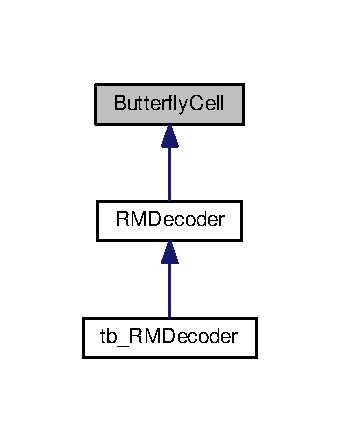
\includegraphics[width=163pt]{class_butterfly_cell__inherit__graph}
\end{center}
\end{figure}
\subsection*{Entities}
\begin{DoxyCompactItemize}
\item 
\hyperlink{class_butterfly_cell_1_1_structural}{Structural} architecture
\end{DoxyCompactItemize}
\subsection*{Libraries}
 \begin{DoxyCompactItemize}
\item 
\hypertarget{class_butterfly_cell_ga0a6af6eef40212dbaf130d57ce711256}{\hyperlink{group___r_m_decoder_ga0a6af6eef40212dbaf130d57ce711256}{ieee} }\label{class_butterfly_cell_ga0a6af6eef40212dbaf130d57ce711256}

\end{DoxyCompactItemize}
\subsection*{Use Clauses}
 \begin{DoxyCompactItemize}
\item 
\hypertarget{class_butterfly_cell_gacd03516902501cd1c7296a98e22c6fcb}{\hyperlink{group___r_m_decoder_gacd03516902501cd1c7296a98e22c6fcb}{std\+\_\+logic\+\_\+1164}   }\label{class_butterfly_cell_gacd03516902501cd1c7296a98e22c6fcb}

\end{DoxyCompactItemize}
\subsection*{Generics}
 \begin{DoxyCompactItemize}
\item 
\hypertarget{class_butterfly_cell_gafe2d022e0ce26a31212f6e0ecf39785d}{\hyperlink{group___r_m_decoder_gafe2d022e0ce26a31212f6e0ecf39785d}{m} {\bfseries {\bfseries \textcolor{vhdlchar}{natural}\textcolor{vhdlchar}{ }\textcolor{vhdlchar}{ }\textcolor{vhdlchar}{\+:}\textcolor{vhdlchar}{=}\textcolor{vhdlchar}{ }\textcolor{vhdlchar}{ } \textcolor{vhdldigit}{3} \textcolor{vhdlchar}{ }}}}\label{class_butterfly_cell_gafe2d022e0ce26a31212f6e0ecf39785d}

\end{DoxyCompactItemize}
\subsection*{Ports}
 \begin{DoxyCompactItemize}
\item 
\hypertarget{class_butterfly_cell_ga2b10c9545b143a051326b4159f5bb7e8}{\hyperlink{group___r_m_decoder_ga2b10c9545b143a051326b4159f5bb7e8}{data\+\_\+in}  {\bfseries {\bfseries \textcolor{vhdlchar}{in}\textcolor{vhdlchar}{ }}} {\bfseries \textcolor{vhdlchar}{std\+\_\+logic\+\_\+vector}\textcolor{vhdlchar}{ }\textcolor{vhdlchar}{(}\textcolor{vhdlchar}{ }\textcolor{vhdlchar}{ } \textcolor{vhdldigit}{2} \textcolor{vhdlchar}{$\ast$}\textcolor{vhdlchar}{$\ast$}\textcolor{vhdlchar}{ }\textcolor{vhdlchar}{ }\textcolor{vhdlchar}{ }\textcolor{vhdlchar}{m}\textcolor{vhdlchar}{-\/}\textcolor{vhdlchar}{ } \textcolor{vhdldigit}{1} \textcolor{vhdlchar}{ }\textcolor{vhdlchar}{downto}\textcolor{vhdlchar}{ }\textcolor{vhdlchar}{ } \textcolor{vhdldigit}{0} \textcolor{vhdlchar}{ }\textcolor{vhdlchar}{)}\textcolor{vhdlchar}{ }} }\label{class_butterfly_cell_ga2b10c9545b143a051326b4159f5bb7e8}

\item 
\hypertarget{class_butterfly_cell_gaa4bbca026b8d1cb018aae06d500d2f54}{\hyperlink{group___r_m_decoder_gaa4bbca026b8d1cb018aae06d500d2f54}{swapped}  {\bfseries {\bfseries \textcolor{vhdlchar}{out}\textcolor{vhdlchar}{ }}} {\bfseries \textcolor{vhdlchar}{std\+\_\+logic\+\_\+vector}\textcolor{vhdlchar}{ }\textcolor{vhdlchar}{(}\textcolor{vhdlchar}{ }\textcolor{vhdlchar}{ } \textcolor{vhdldigit}{2} \textcolor{vhdlchar}{$\ast$}\textcolor{vhdlchar}{$\ast$}\textcolor{vhdlchar}{ }\textcolor{vhdlchar}{ }\textcolor{vhdlchar}{ }\textcolor{vhdlchar}{m}\textcolor{vhdlchar}{-\/}\textcolor{vhdlchar}{ } \textcolor{vhdldigit}{1} \textcolor{vhdlchar}{ }\textcolor{vhdlchar}{downto}\textcolor{vhdlchar}{ }\textcolor{vhdlchar}{ } \textcolor{vhdldigit}{0} \textcolor{vhdlchar}{ }\textcolor{vhdlchar}{)}\textcolor{vhdlchar}{ }} }\label{class_butterfly_cell_gaa4bbca026b8d1cb018aae06d500d2f54}

\end{DoxyCompactItemize}


\subsection{Descrizione dettagliata}
implementazione V\+H\+D\+L dello swap usato nel decodificatore di Reed-\/\+Muller 

Il componente \hyperlink{class_butterfly_cell}{Butterfly\+Cell} implementa la rete di swap necessarie al'implementazione del decodificatore a maggioranza per i codici di Reed-\/\+Muller R\+M(1, m). Il componente ha un'implementazione parametrica, il che permette di usare lo stesso componente qualsiasi sia il parametro \char`\"{}m\char`\"{}.


\begin{DoxyParams}{Parametri}
{\em m} & parametro \char`\"{}m\char`\"{} del codice di Reed-\/\+Muller usato. \\
\hline
{\em data\+\_\+in\mbox{[}in\mbox{]}} & vettore contenente il codice di Reed-\/\+Muller da swappare. Il parallelismo e' 2$^\wedge$m -\/ 1 \\
\hline
{\em swapped\mbox{[}out\mbox{]}} & vettore che conterra' il risultato delle operazioni di swapping del vettore data\+\_\+in \\
\hline
\end{DoxyParams}


La documentazione per questa classe è stata generata a partire dal seguente file\+:\begin{DoxyCompactItemize}
\item 
R\+M\+Decoder/\hyperlink{_butterfly_cell_8vhd}{Butterfly\+Cell.\+vhd}\end{DoxyCompactItemize}

\hypertarget{classcomparator2bit}{\section{comparator2bit Entity Reference}
\label{classcomparator2bit}\index{comparator2bit@{comparator2bit}}
}


Implementazione V\+H\+D\+L Data Flow di un comparatore a 2 bit che tiene conto anche del risutato di un confronto precedente.  




Diagramma delle classi per comparator2bit\nopagebreak
\begin{figure}[H]
\begin{center}
\leavevmode
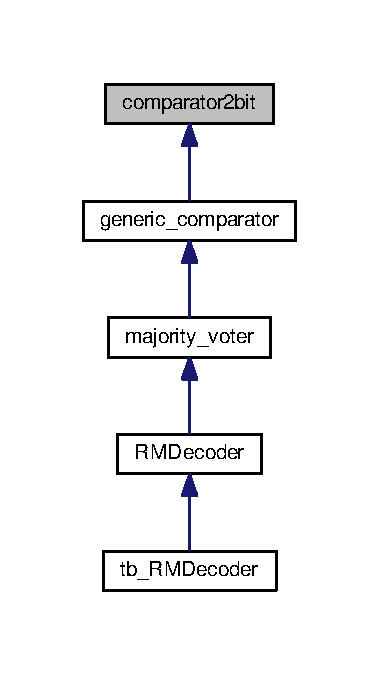
\includegraphics[width=182pt]{classcomparator2bit__inherit__graph}
\end{center}
\end{figure}
\subsection*{Entities}
\begin{DoxyCompactItemize}
\item 
\hyperlink{classcomparator2bit_1_1_data_flow}{Data\+Flow} architecture
\end{DoxyCompactItemize}
\subsection*{Libraries}
 \begin{DoxyCompactItemize}
\item 
\hypertarget{classcomparator2bit_gae4f03c286607f3181e16b9aa12d0c6d4}{\hyperlink{group___majority_voter_gae4f03c286607f3181e16b9aa12d0c6d4}{I\+E\+E\+E} }\label{classcomparator2bit_gae4f03c286607f3181e16b9aa12d0c6d4}

\end{DoxyCompactItemize}
\subsection*{Use Clauses}
 \begin{DoxyCompactItemize}
\item 
\hypertarget{classcomparator2bit_gaa4b2b25246a821511120e3149b003563}{\hyperlink{group___majority_voter_gaa4b2b25246a821511120e3149b003563}{S\+T\+D\+\_\+\+L\+O\+G\+I\+C\+\_\+1164}   }\label{classcomparator2bit_gaa4b2b25246a821511120e3149b003563}

\end{DoxyCompactItemize}
\subsection*{Ports}
 \begin{DoxyCompactItemize}
\item 
\hypertarget{classcomparator2bit_gae267849523b1c1f9f7ec27e888f16b76}{\hyperlink{group___majority_voter_gae267849523b1c1f9f7ec27e888f16b76}{a}  {\bfseries {\bfseries \textcolor{vhdlchar}{in}\textcolor{vhdlchar}{ }}} {\bfseries \textcolor{vhdlchar}{S\+T\+D\+\_\+\+L\+O\+G\+I\+C}\textcolor{vhdlchar}{ }} }\label{classcomparator2bit_gae267849523b1c1f9f7ec27e888f16b76}

\item 
\hypertarget{classcomparator2bit_ga07cae6968507bccfad6a655cd6d5c709}{\hyperlink{group___majority_voter_ga07cae6968507bccfad6a655cd6d5c709}{b}  {\bfseries {\bfseries \textcolor{vhdlchar}{in}\textcolor{vhdlchar}{ }}} {\bfseries \textcolor{vhdlchar}{S\+T\+D\+\_\+\+L\+O\+G\+I\+C}\textcolor{vhdlchar}{ }} }\label{classcomparator2bit_ga07cae6968507bccfad6a655cd6d5c709}

\item 
\hypertarget{classcomparator2bit_gaa9dd88146339eb59a852432f2ac9b902}{\hyperlink{group___majority_voter_gaa9dd88146339eb59a852432f2ac9b902}{res\+\_\+in}  {\bfseries {\bfseries \textcolor{vhdlchar}{in}\textcolor{vhdlchar}{ }}} {\bfseries \textcolor{vhdlchar}{S\+T\+D\+\_\+\+L\+O\+G\+I\+C}\textcolor{vhdlchar}{ }} }\label{classcomparator2bit_gaa9dd88146339eb59a852432f2ac9b902}

\item 
\hypertarget{classcomparator2bit_gab3e0985b4eabe8ffdbb4b06c5396c438}{\hyperlink{group___majority_voter_gab3e0985b4eabe8ffdbb4b06c5396c438}{res\+\_\+out}  {\bfseries {\bfseries \textcolor{vhdlchar}{out}\textcolor{vhdlchar}{ }}} {\bfseries \textcolor{vhdlchar}{S\+T\+D\+\_\+\+L\+O\+G\+I\+C}\textcolor{vhdlchar}{ }} }\label{classcomparator2bit_gab3e0985b4eabe8ffdbb4b06c5396c438}

\end{DoxyCompactItemize}


\subsection{Descrizione dettagliata}
Implementazione V\+H\+D\+L Data Flow di un comparatore a 2 bit che tiene conto anche del risutato di un confronto precedente. 


\begin{DoxyParams}{Parametri}
{\em a\mbox{[}in\mbox{]}} & ingresso 1 \\
\hline
{\em b\mbox{[}in\mbox{]}} & ingresso 2 \\
\hline
{\em res\+\_\+in\mbox{[}in\mbox{]}} & risultato del confronto precedente \\
\hline
{\em res\+\_\+out\mbox{[}in\mbox{]}} & risultato del confronto \\
\hline
\end{DoxyParams}


La documentazione per questa classe è stata generata a partire dal seguente file\+:\begin{DoxyCompactItemize}
\item 
R\+M\+Decoder/\+Majority\+Voter/\hyperlink{comparator2bit_8vhd}{comparator2bit.\+vhd}\end{DoxyCompactItemize}

\hypertarget{classcomparator2bit_1_1_data_flow}{\section{Data\+Flow Architecture Reference}
\label{classcomparator2bit_1_1_data_flow}\index{Data\+Flow@{Data\+Flow}}
}
\subsection*{Signals}
 \begin{DoxyCompactItemize}
\item 
\hypertarget{classcomparator2bit_1_1_data_flow_ga052a90adf60bb3fc0352fc16b4d22cc6}{\hyperlink{group___majority_voter_ga052a90adf60bb3fc0352fc16b4d22cc6}{tmp1} {\bfseries \textcolor{vhdlchar}{std\+\_\+logic}\textcolor{vhdlchar}{ }\textcolor{vhdlchar}{ }\textcolor{vhdlchar}{\+:}\textcolor{vhdlchar}{=}\textcolor{vhdlchar}{ }\textcolor{vhdlchar}{ }\textcolor{vhdlchar}{'}\textcolor{vhdlchar}{ } \textcolor{vhdldigit}{0} \textcolor{vhdlchar}{ }\textcolor{vhdlchar}{'}\textcolor{vhdlchar}{ }} }\label{classcomparator2bit_1_1_data_flow_ga052a90adf60bb3fc0352fc16b4d22cc6}

\item 
\hypertarget{classcomparator2bit_1_1_data_flow_gaa2bb8e3a49b58e114167a4a35318f363}{\hyperlink{group___majority_voter_gaa2bb8e3a49b58e114167a4a35318f363}{tmp2} {\bfseries \textcolor{vhdlchar}{std\+\_\+logic}\textcolor{vhdlchar}{ }\textcolor{vhdlchar}{ }\textcolor{vhdlchar}{\+:}\textcolor{vhdlchar}{=}\textcolor{vhdlchar}{ }\textcolor{vhdlchar}{ }\textcolor{vhdlchar}{'}\textcolor{vhdlchar}{ } \textcolor{vhdldigit}{0} \textcolor{vhdlchar}{ }\textcolor{vhdlchar}{'}\textcolor{vhdlchar}{ }} }\label{classcomparator2bit_1_1_data_flow_gaa2bb8e3a49b58e114167a4a35318f363}

\item 
\hypertarget{classcomparator2bit_1_1_data_flow_ga9f50761ba7cfe80836abd801ef32b402}{\hyperlink{group___majority_voter_ga9f50761ba7cfe80836abd801ef32b402}{tmp3} {\bfseries \textcolor{vhdlchar}{std\+\_\+logic}\textcolor{vhdlchar}{ }\textcolor{vhdlchar}{ }\textcolor{vhdlchar}{\+:}\textcolor{vhdlchar}{=}\textcolor{vhdlchar}{ }\textcolor{vhdlchar}{ }\textcolor{vhdlchar}{'}\textcolor{vhdlchar}{ } \textcolor{vhdldigit}{0} \textcolor{vhdlchar}{ }\textcolor{vhdlchar}{'}\textcolor{vhdlchar}{ }} }\label{classcomparator2bit_1_1_data_flow_ga9f50761ba7cfe80836abd801ef32b402}

\end{DoxyCompactItemize}


La documentazione per questa classe è stata generata a partire dal seguente file\+:\begin{DoxyCompactItemize}
\item 
R\+M\+Decoder/\+Majority\+Voter/\hyperlink{comparator2bit_8vhd}{comparator2bit.\+vhd}\end{DoxyCompactItemize}

\hypertarget{classfull__adder_1_1_data_flow}{\section{Data\+Flow Architecture Reference}
\label{classfull__adder_1_1_data_flow}\index{Data\+Flow@{Data\+Flow}}
}


La documentazione per questa classe è stata generata a partire dal seguente file\+:\begin{DoxyCompactItemize}
\item 
R\+M\+Decoder/\+Majority\+Voter/\hyperlink{full__adder_8vhd}{full\+\_\+adder.\+vhd}\end{DoxyCompactItemize}

\hypertarget{classfull__adder}{\section{full\+\_\+adder Entity Reference}
\label{classfull__adder}\index{full\+\_\+adder@{full\+\_\+adder}}
}


Diagramma delle classi per full\+\_\+adder\nopagebreak
\begin{figure}[H]
\begin{center}
\leavevmode
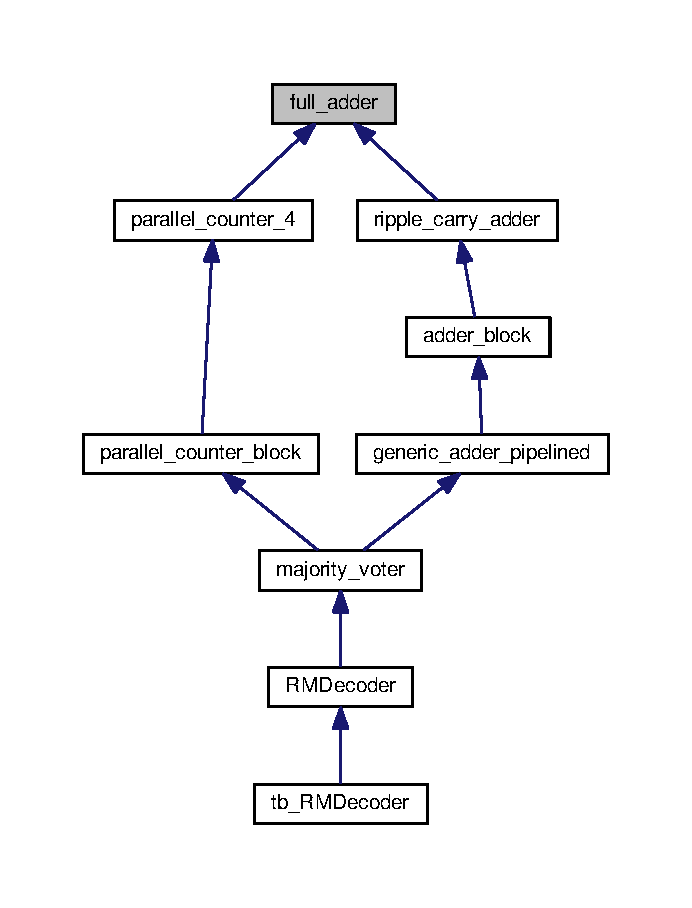
\includegraphics[width=332pt]{classfull__adder__inherit__graph}
\end{center}
\end{figure}
\subsection*{Entities}
\begin{DoxyCompactItemize}
\item 
\hyperlink{classfull__adder_1_1_data_flow}{Data\+Flow} architecture
\end{DoxyCompactItemize}
\subsection*{Libraries}
 \begin{DoxyCompactItemize}
\item 
\hypertarget{classfull__adder_gae4f03c286607f3181e16b9aa12d0c6d4}{\hyperlink{group___majority_voter_gae4f03c286607f3181e16b9aa12d0c6d4}{I\+E\+E\+E} }\label{classfull__adder_gae4f03c286607f3181e16b9aa12d0c6d4}

\end{DoxyCompactItemize}
\subsection*{Use Clauses}
 \begin{DoxyCompactItemize}
\item 
\hypertarget{classfull__adder_gaa4b2b25246a821511120e3149b003563}{\hyperlink{group___majority_voter_gaa4b2b25246a821511120e3149b003563}{S\+T\+D\+\_\+\+L\+O\+G\+I\+C\+\_\+1164}   }\label{classfull__adder_gaa4b2b25246a821511120e3149b003563}

\end{DoxyCompactItemize}
\subsection*{Ports}
 \begin{DoxyCompactItemize}
\item 
\hypertarget{classfull__adder_ga3d6cfc8eb92a4fa7bd17df688efa5522}{\hyperlink{group___majority_voter_ga3d6cfc8eb92a4fa7bd17df688efa5522}{add\+\_\+1}  {\bfseries {\bfseries \textcolor{vhdlchar}{in}\textcolor{vhdlchar}{ }}} {\bfseries \textcolor{vhdlchar}{S\+T\+D\+\_\+\+L\+O\+G\+I\+C}\textcolor{vhdlchar}{ }} }\label{classfull__adder_ga3d6cfc8eb92a4fa7bd17df688efa5522}

\item 
\hypertarget{classfull__adder_gaf7639b8ec31b7bb5b1d72d1796d5833e}{\hyperlink{group___majority_voter_gaf7639b8ec31b7bb5b1d72d1796d5833e}{add\+\_\+2}  {\bfseries {\bfseries \textcolor{vhdlchar}{in}\textcolor{vhdlchar}{ }}} {\bfseries \textcolor{vhdlchar}{S\+T\+D\+\_\+\+L\+O\+G\+I\+C}\textcolor{vhdlchar}{ }} }\label{classfull__adder_gaf7639b8ec31b7bb5b1d72d1796d5833e}

\item 
\hypertarget{classfull__adder_gab93e0e530f7cfe8f44daa9285209cca1}{\hyperlink{group___majority_voter_gab93e0e530f7cfe8f44daa9285209cca1}{carry\+\_\+in}  {\bfseries {\bfseries \textcolor{vhdlchar}{in}\textcolor{vhdlchar}{ }}} {\bfseries \textcolor{vhdlchar}{S\+T\+D\+\_\+\+L\+O\+G\+I\+C}\textcolor{vhdlchar}{ }} }\label{classfull__adder_gab93e0e530f7cfe8f44daa9285209cca1}

\item 
\hypertarget{classfull__adder_gafcc7c006376592bcf77bccdcfd0a99bc}{\hyperlink{group___majority_voter_gafcc7c006376592bcf77bccdcfd0a99bc}{carry\+\_\+out}  {\bfseries {\bfseries \textcolor{vhdlchar}{out}\textcolor{vhdlchar}{ }}} {\bfseries \textcolor{vhdlchar}{S\+T\+D\+\_\+\+L\+O\+G\+I\+C}\textcolor{vhdlchar}{ }} }\label{classfull__adder_gafcc7c006376592bcf77bccdcfd0a99bc}

\item 
\hypertarget{classfull__adder_ga869bdd6b2525c2745b2cc24818de1a72}{\hyperlink{group___majority_voter_ga869bdd6b2525c2745b2cc24818de1a72}{sum}  {\bfseries {\bfseries \textcolor{vhdlchar}{out}\textcolor{vhdlchar}{ }}} {\bfseries \textcolor{vhdlchar}{S\+T\+D\+\_\+\+L\+O\+G\+I\+C}\textcolor{vhdlchar}{ }} }\label{classfull__adder_ga869bdd6b2525c2745b2cc24818de1a72}

\end{DoxyCompactItemize}


La documentazione per questa classe è stata generata a partire dal seguente file\+:\begin{DoxyCompactItemize}
\item 
R\+M\+Decoder/\+Majority\+Voter/\hyperlink{full__adder_8vhd}{full\+\_\+adder.\+vhd}\end{DoxyCompactItemize}

\hypertarget{classgeneric__adder__pipelined}{\section{generic\+\_\+adder\+\_\+pipelined Entity Reference}
\label{classgeneric__adder__pipelined}\index{generic\+\_\+adder\+\_\+pipelined@{generic\+\_\+adder\+\_\+pipelined}}
}


Implementazione V\+H\+D\+L \hyperlink{classgeneric__adder__pipelined_1_1_structural}{Structural} di un addizionatore generico pipelined \+: M operandi di N bit.  




Diagramma delle classi per generic\+\_\+adder\+\_\+pipelined\nopagebreak
\begin{figure}[H]
\begin{center}
\leavevmode
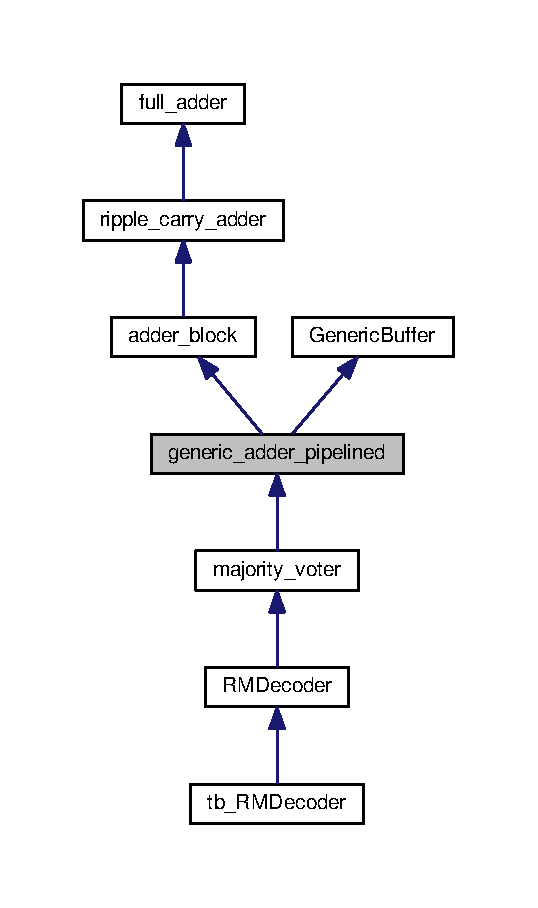
\includegraphics[width=258pt]{classgeneric__adder__pipelined__inherit__graph}
\end{center}
\end{figure}


Diagramma di collaborazione per generic\+\_\+adder\+\_\+pipelined\+:\nopagebreak
\begin{figure}[H]
\begin{center}
\leavevmode
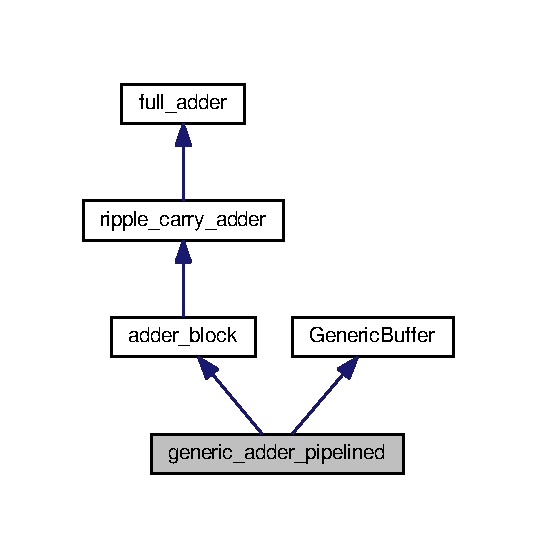
\includegraphics[width=258pt]{classgeneric__adder__pipelined__coll__graph}
\end{center}
\end{figure}
\subsection*{Entities}
\begin{DoxyCompactItemize}
\item 
\hyperlink{classgeneric__adder__pipelined_1_1_structural}{Structural} architecture
\end{DoxyCompactItemize}
\subsection*{Libraries}
 \begin{DoxyCompactItemize}
\item 
\hypertarget{classgeneric__adder__pipelined_gae4f03c286607f3181e16b9aa12d0c6d4}{\hyperlink{group___majority_voter_gae4f03c286607f3181e16b9aa12d0c6d4}{I\+E\+E\+E} }\label{classgeneric__adder__pipelined_gae4f03c286607f3181e16b9aa12d0c6d4}

\end{DoxyCompactItemize}
\subsection*{Use Clauses}
 \begin{DoxyCompactItemize}
\item 
\hypertarget{classgeneric__adder__pipelined_gaa4b2b25246a821511120e3149b003563}{\hyperlink{group___majority_voter_gaa4b2b25246a821511120e3149b003563}{S\+T\+D\+\_\+\+L\+O\+G\+I\+C\+\_\+1164}   }\label{classgeneric__adder__pipelined_gaa4b2b25246a821511120e3149b003563}

\item 
\hypertarget{classgeneric__adder__pipelined_gae00f3f04545af57582ff10609eee23e2}{\hyperlink{group___majority_voter_gae00f3f04545af57582ff10609eee23e2}{N\+U\+M\+E\+R\+I\+C\+\_\+\+S\+T\+D}   }\label{classgeneric__adder__pipelined_gae00f3f04545af57582ff10609eee23e2}

\item 
\hypertarget{classgeneric__adder__pipelined_ga6af860958a1bb510ee63ced87b57e11a}{\hyperlink{group___majority_voter_ga6af860958a1bb510ee63ced87b57e11a}{M\+A\+T\+H\+\_\+\+R\+E\+A\+L}   }\label{classgeneric__adder__pipelined_ga6af860958a1bb510ee63ced87b57e11a}

\end{DoxyCompactItemize}
\subsection*{Generics}
 \begin{DoxyCompactItemize}
\item 
\hypertarget{classgeneric__adder__pipelined_ga391d71eb279c0942fd4f72f35110ebcf}{\hyperlink{group___majority_voter_ga391d71eb279c0942fd4f72f35110ebcf}{number\+\_\+operand} {\bfseries {\bfseries \textcolor{vhdlchar}{N\+A\+T\+U\+R\+A\+L}\textcolor{vhdlchar}{ }\textcolor{vhdlchar}{ }\textcolor{vhdlchar}{\+:}\textcolor{vhdlchar}{=}\textcolor{vhdlchar}{ }\textcolor{vhdlchar}{ } \textcolor{vhdldigit}{2} \textcolor{vhdlchar}{ }}}}\label{classgeneric__adder__pipelined_ga391d71eb279c0942fd4f72f35110ebcf}

\item 
\hypertarget{classgeneric__adder__pipelined_gae919dbd8a1b11697f75ab57736802493}{\hyperlink{group___majority_voter_gae919dbd8a1b11697f75ab57736802493}{number\+\_\+bit\+\_\+for\+\_\+operand} {\bfseries {\bfseries \textcolor{vhdlchar}{N\+A\+T\+U\+R\+A\+L}\textcolor{vhdlchar}{ }\textcolor{vhdlchar}{ }\textcolor{vhdlchar}{\+:}\textcolor{vhdlchar}{=}\textcolor{vhdlchar}{ }\textcolor{vhdlchar}{ } \textcolor{vhdldigit}{3} \textcolor{vhdlchar}{ }}}}\label{classgeneric__adder__pipelined_gae919dbd8a1b11697f75ab57736802493}

\end{DoxyCompactItemize}
\subsection*{Ports}
 \begin{DoxyCompactItemize}
\item 
\hypertarget{classgeneric__adder__pipelined_ga6231b307b7958b6060563aa2a93d345a}{\hyperlink{group___majority_voter_ga6231b307b7958b6060563aa2a93d345a}{clk}  {\bfseries {\bfseries \textcolor{vhdlchar}{in}\textcolor{vhdlchar}{ }}} {\bfseries \textcolor{vhdlchar}{S\+T\+D\+\_\+\+L\+O\+G\+I\+C}\textcolor{vhdlchar}{ }} }\label{classgeneric__adder__pipelined_ga6231b307b7958b6060563aa2a93d345a}

\item 
\hypertarget{classgeneric__adder__pipelined_ga8881084de0fcf748e41bd0fd1028445e}{\hyperlink{group___majority_voter_ga8881084de0fcf748e41bd0fd1028445e}{reset\+\_\+n}  {\bfseries {\bfseries \textcolor{vhdlchar}{in}\textcolor{vhdlchar}{ }}} {\bfseries \textcolor{vhdlchar}{S\+T\+D\+\_\+\+L\+O\+G\+I\+C}\textcolor{vhdlchar}{ }} }\label{classgeneric__adder__pipelined_ga8881084de0fcf748e41bd0fd1028445e}

\item 
\hypertarget{classgeneric__adder__pipelined_ga359e3b0c94c0e1466b7a2b503b3623be}{\hyperlink{group___majority_voter_ga359e3b0c94c0e1466b7a2b503b3623be}{data\+\_\+in}  {\bfseries {\bfseries \textcolor{vhdlchar}{in}\textcolor{vhdlchar}{ }}} {\bfseries \textcolor{vhdlchar}{S\+T\+D\+\_\+\+L\+O\+G\+I\+C\+\_\+\+V\+E\+C\+T\+O\+R}\textcolor{vhdlchar}{ }\textcolor{vhdlchar}{(}\textcolor{vhdlchar}{ }\textcolor{vhdlchar}{(}\textcolor{vhdlchar}{ }\textcolor{vhdlchar}{ }\textcolor{vhdlchar}{ }\textcolor{vhdlchar}{ }\textcolor{vhdlchar}{number\+\_\+operand}\textcolor{vhdlchar}{$\ast$}\textcolor{vhdlchar}{ }\textcolor{vhdlchar}{ }\textcolor{vhdlchar}{ }\textcolor{vhdlchar}{number\+\_\+bit\+\_\+for\+\_\+operand}\textcolor{vhdlchar}{ }\textcolor{vhdlchar}{)}\textcolor{vhdlchar}{ }\textcolor{vhdlchar}{-\/}\textcolor{vhdlchar}{ } \textcolor{vhdldigit}{1} \textcolor{vhdlchar}{ }\textcolor{vhdlchar}{downto}\textcolor{vhdlchar}{ }\textcolor{vhdlchar}{ } \textcolor{vhdldigit}{0} \textcolor{vhdlchar}{ }\textcolor{vhdlchar}{)}\textcolor{vhdlchar}{ }} }\label{classgeneric__adder__pipelined_ga359e3b0c94c0e1466b7a2b503b3623be}

\item 
\hypertarget{classgeneric__adder__pipelined_ga7087cf66799b189f1ad9c93f82a39a50}{\hyperlink{group___majority_voter_ga7087cf66799b189f1ad9c93f82a39a50}{data\+\_\+out}  {\bfseries {\bfseries \textcolor{vhdlchar}{out}\textcolor{vhdlchar}{ }}} {\bfseries \textcolor{vhdlchar}{S\+T\+D\+\_\+\+L\+O\+G\+I\+C\+\_\+\+V\+E\+C\+T\+O\+R}\textcolor{vhdlchar}{ }\textcolor{vhdlchar}{(}\textcolor{vhdlchar}{ }\textcolor{vhdlchar}{(}\textcolor{vhdlchar}{ }\textcolor{vhdlchar}{ }\textcolor{vhdlchar}{ }\textcolor{vhdlchar}{ }\textcolor{vhdlchar}{number\+\_\+bit\+\_\+for\+\_\+operand}\textcolor{vhdlchar}{+}\textcolor{vhdlchar}{ }\textcolor{vhdlchar}{ }\textcolor{vhdlchar}{ }\textcolor{vhdlchar}{natural}\textcolor{vhdlchar}{ }\textcolor{vhdlchar}{(}\textcolor{vhdlchar}{ }\textcolor{vhdlchar}{log2}\textcolor{vhdlchar}{ }\textcolor{vhdlchar}{(}\textcolor{vhdlchar}{ }\textcolor{vhdlchar}{real}\textcolor{vhdlchar}{ }\textcolor{vhdlchar}{(}\textcolor{vhdlchar}{ }\textcolor{vhdlchar}{number\+\_\+operand}\textcolor{vhdlchar}{ }\textcolor{vhdlchar}{ }\textcolor{vhdlchar}{)}\textcolor{vhdlchar}{ }\textcolor{vhdlchar}{ }\textcolor{vhdlchar}{ }\textcolor{vhdlchar}{)}\textcolor{vhdlchar}{ }\textcolor{vhdlchar}{ }\textcolor{vhdlchar}{ }\textcolor{vhdlchar}{)}\textcolor{vhdlchar}{ }\textcolor{vhdlchar}{)}\textcolor{vhdlchar}{ }\textcolor{vhdlchar}{-\/}\textcolor{vhdlchar}{ } \textcolor{vhdldigit}{1} \textcolor{vhdlchar}{ }\textcolor{vhdlchar}{downto}\textcolor{vhdlchar}{ }\textcolor{vhdlchar}{ } \textcolor{vhdldigit}{0} \textcolor{vhdlchar}{ }\textcolor{vhdlchar}{)}\textcolor{vhdlchar}{ }} }\label{classgeneric__adder__pipelined_ga7087cf66799b189f1ad9c93f82a39a50}

\end{DoxyCompactItemize}


\subsection{Descrizione dettagliata}
Implementazione V\+H\+D\+L \hyperlink{classgeneric__adder__pipelined_1_1_structural}{Structural} di un addizionatore generico pipelined \+: M operandi di N bit. 


\begin{DoxyParams}{Parametri}
{\em number\+\_\+operand\mbox{[}in\mbox{]}} & parametro che determina il numero di operandi dell' addizionatore \\
\hline
{\em number\+\_\+bit\+\_\+for\+\_\+operand\mbox{[}in\mbox{]}} & parametro che determina il numero di bit di ogni operando\\
\hline
{\em clk\mbox{[}in\mbox{]}} & segnale di clock \\
\hline
{\em reset\+\_\+n\mbox{[}in\mbox{]}} & segnale di reset asincrono, attivo basso \\
\hline
{\em data\+\_\+in\mbox{[}in\mbox{]}} & stringa di bit di input di dimensione (number\+\_\+operand $\ast$ number\+\_\+bit\+\_\+for\+\_\+operand) che è la concatenzaione degli operandi da sommare \\
\hline
{\em data\+\_\+out\mbox{[}out\mbox{]}} & stringa di bit di uscita di dimensione (number\+\_\+bit\+\_\+for\+\_\+operand + natural(log2(real(number\+\_\+operand)))) che è la somma totale degli operandi di ingresso \\
\hline
\end{DoxyParams}


La documentazione per questa classe è stata generata a partire dal seguente file\+:\begin{DoxyCompactItemize}
\item 
R\+M\+Decoder/\+Majority\+Voter/\hyperlink{generic__adder__pipelined_8vhd}{generic\+\_\+adder\+\_\+pipelined.\+vhd}\end{DoxyCompactItemize}

\hypertarget{classgeneric__comparator}{\section{generic\+\_\+comparator Entity Reference}
\label{classgeneric__comparator}\index{generic\+\_\+comparator@{generic\+\_\+comparator}}
}


Implementazione V\+H\+D\+L \hyperlink{classgeneric__comparator_1_1_structural}{Structural} di un generico comparatore a maggioranza di due stringhe di width bit. Tale implementazione genera una catena di \char`\"{}width\char`\"{} comparatori a 2 bit.  




Diagramma delle classi per generic\+\_\+comparator\nopagebreak
\begin{figure}[H]
\begin{center}
\leavevmode
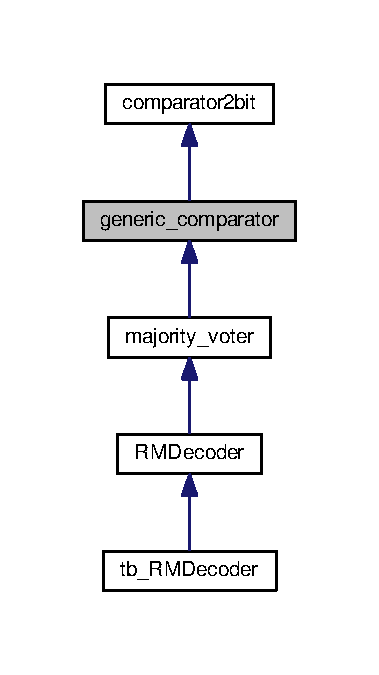
\includegraphics[width=182pt]{classgeneric__comparator__inherit__graph}
\end{center}
\end{figure}


Diagramma di collaborazione per generic\+\_\+comparator\+:\nopagebreak
\begin{figure}[H]
\begin{center}
\leavevmode
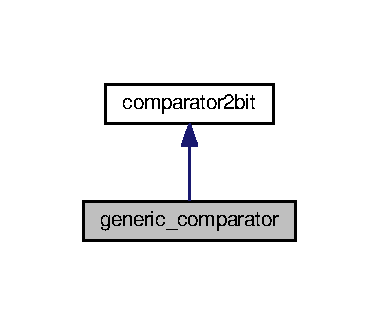
\includegraphics[width=182pt]{classgeneric__comparator__coll__graph}
\end{center}
\end{figure}
\subsection*{Entities}
\begin{DoxyCompactItemize}
\item 
\hyperlink{classgeneric__comparator_1_1_structural}{Structural} architecture
\end{DoxyCompactItemize}
\subsection*{Libraries}
 \begin{DoxyCompactItemize}
\item 
\hypertarget{classgeneric__comparator_gae4f03c286607f3181e16b9aa12d0c6d4}{\hyperlink{group___majority_voter_gae4f03c286607f3181e16b9aa12d0c6d4}{I\+E\+E\+E} }\label{classgeneric__comparator_gae4f03c286607f3181e16b9aa12d0c6d4}

\end{DoxyCompactItemize}
\subsection*{Use Clauses}
 \begin{DoxyCompactItemize}
\item 
\hypertarget{classgeneric__comparator_gaa4b2b25246a821511120e3149b003563}{\hyperlink{group___majority_voter_gaa4b2b25246a821511120e3149b003563}{S\+T\+D\+\_\+\+L\+O\+G\+I\+C\+\_\+1164}   }\label{classgeneric__comparator_gaa4b2b25246a821511120e3149b003563}

\end{DoxyCompactItemize}
\subsection*{Generics}
 \begin{DoxyCompactItemize}
\item 
\hypertarget{classgeneric__comparator_ga93ec5006d2e0a77a21f35a7e3c1ca827}{\hyperlink{group___majority_voter_ga93ec5006d2e0a77a21f35a7e3c1ca827}{width} {\bfseries {\bfseries \textcolor{vhdlchar}{N\+A\+T\+U\+R\+A\+L}\textcolor{vhdlchar}{ }\textcolor{vhdlchar}{ }\textcolor{vhdlchar}{\+:}\textcolor{vhdlchar}{=}\textcolor{vhdlchar}{ }\textcolor{vhdlchar}{ } \textcolor{vhdldigit}{8} \textcolor{vhdlchar}{ }}}}\label{classgeneric__comparator_ga93ec5006d2e0a77a21f35a7e3c1ca827}

\end{DoxyCompactItemize}
\subsection*{Ports}
 \begin{DoxyCompactItemize}
\item 
\hypertarget{classgeneric__comparator_gaafe8d8f538bf4e2bdb9b8a73b793dad7}{\hyperlink{group___majority_voter_gaafe8d8f538bf4e2bdb9b8a73b793dad7}{data\+\_\+in}  {\bfseries {\bfseries \textcolor{vhdlchar}{in}\textcolor{vhdlchar}{ }}} {\bfseries \textcolor{vhdlchar}{S\+T\+D\+\_\+\+L\+O\+G\+I\+C\+\_\+\+V\+E\+C\+T\+O\+R}\textcolor{vhdlchar}{ }\textcolor{vhdlchar}{(}\textcolor{vhdlchar}{ }\textcolor{vhdlchar}{ }\textcolor{vhdlchar}{ }\textcolor{vhdlchar}{ }\textcolor{vhdlchar}{width}\textcolor{vhdlchar}{-\/}\textcolor{vhdlchar}{ } \textcolor{vhdldigit}{1} \textcolor{vhdlchar}{ }\textcolor{vhdlchar}{downto}\textcolor{vhdlchar}{ }\textcolor{vhdlchar}{ } \textcolor{vhdldigit}{0} \textcolor{vhdlchar}{ }\textcolor{vhdlchar}{)}\textcolor{vhdlchar}{ }} }\label{classgeneric__comparator_gaafe8d8f538bf4e2bdb9b8a73b793dad7}

\item 
\hypertarget{classgeneric__comparator_ga9237ccbc80d19822650f7ef1180770fd}{\hyperlink{group___majority_voter_ga9237ccbc80d19822650f7ef1180770fd}{data\+\_\+cmp}  {\bfseries {\bfseries \textcolor{vhdlchar}{in}\textcolor{vhdlchar}{ }}} {\bfseries \textcolor{vhdlchar}{S\+T\+D\+\_\+\+L\+O\+G\+I\+C\+\_\+\+V\+E\+C\+T\+O\+R}\textcolor{vhdlchar}{ }\textcolor{vhdlchar}{(}\textcolor{vhdlchar}{ }\textcolor{vhdlchar}{ }\textcolor{vhdlchar}{ }\textcolor{vhdlchar}{ }\textcolor{vhdlchar}{width}\textcolor{vhdlchar}{-\/}\textcolor{vhdlchar}{ } \textcolor{vhdldigit}{1} \textcolor{vhdlchar}{ }\textcolor{vhdlchar}{downto}\textcolor{vhdlchar}{ }\textcolor{vhdlchar}{ } \textcolor{vhdldigit}{0} \textcolor{vhdlchar}{ }\textcolor{vhdlchar}{)}\textcolor{vhdlchar}{ }} }\label{classgeneric__comparator_ga9237ccbc80d19822650f7ef1180770fd}

\item 
\hypertarget{classgeneric__comparator_gab78b887b4d5060c44e453704d8846372}{\hyperlink{group___majority_voter_gab78b887b4d5060c44e453704d8846372}{data\+\_\+out}  {\bfseries {\bfseries \textcolor{vhdlchar}{out}\textcolor{vhdlchar}{ }}} {\bfseries \textcolor{vhdlchar}{S\+T\+D\+\_\+\+L\+O\+G\+I\+C}\textcolor{vhdlchar}{ }} }\label{classgeneric__comparator_gab78b887b4d5060c44e453704d8846372}

\end{DoxyCompactItemize}


\subsection{Descrizione dettagliata}
Implementazione V\+H\+D\+L \hyperlink{classgeneric__comparator_1_1_structural}{Structural} di un generico comparatore a maggioranza di due stringhe di width bit. Tale implementazione genera una catena di \char`\"{}width\char`\"{} comparatori a 2 bit. 


\begin{DoxyParams}{Parametri}
{\em width\mbox{[}in\mbox{]}} & parametro che determina la dimensione del comparatore\\
\hline
{\em data\+\_\+in\mbox{[}in\mbox{]}} & stringa di bit di input di dimensione width \\
\hline
{\em data\+\_\+cmp\mbox{[}in\mbox{]}} & stringa di bit di input di dimensione width \\
\hline
{\em data\+\_\+out\mbox{[}out\mbox{]}} & risultato del confronto\+: data\+\_\+out = 1 se data\+\_\+in $>$ data\+\_\+cmp data\+\_\+out = 0 altrimenti \\
\hline
\end{DoxyParams}


La documentazione per questa classe è stata generata a partire dal seguente file\+:\begin{DoxyCompactItemize}
\item 
R\+M\+Decoder/\+Majority\+Voter/\hyperlink{generic__comparator_8vhd}{generic\+\_\+comparator.\+vhd}\end{DoxyCompactItemize}

\hypertarget{class_generic_buffer}{\section{Generic\+Buffer Entity Reference}
\label{class_generic_buffer}\index{Generic\+Buffer@{Generic\+Buffer}}
}


Registro di dimensione generica.  




Diagramma delle classi per Generic\+Buffer\nopagebreak
\begin{figure}[H]
\begin{center}
\leavevmode
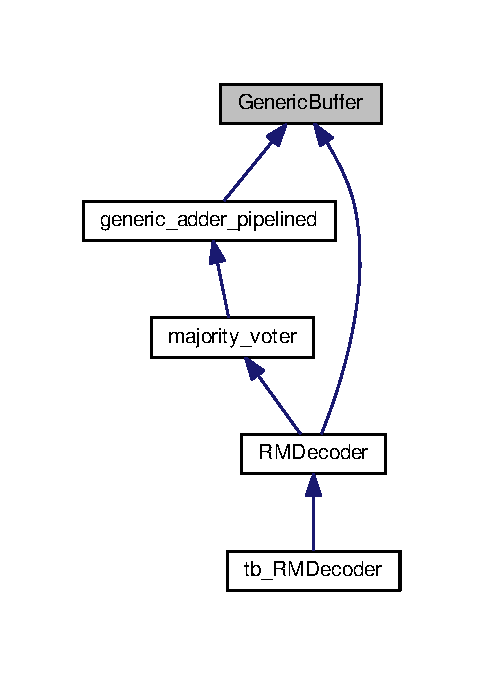
\includegraphics[width=232pt]{class_generic_buffer__inherit__graph}
\end{center}
\end{figure}
\subsection*{Entities}
\begin{DoxyCompactItemize}
\item 
\hyperlink{class_generic_buffer_1_1_behavioral}{Behavioral} architecture
\end{DoxyCompactItemize}
\subsection*{Libraries}
 \begin{DoxyCompactItemize}
\item 
\hyperlink{class_generic_buffer_a0a6af6eef40212dbaf130d57ce711256}{ieee} 
\end{DoxyCompactItemize}
\subsection*{Use Clauses}
 \begin{DoxyCompactItemize}
\item 
\hypertarget{class_generic_buffer_gacd03516902501cd1c7296a98e22c6fcb}{\hyperlink{group___r_m_decoder_gacd03516902501cd1c7296a98e22c6fcb}{std\+\_\+logic\+\_\+1164}   }\label{class_generic_buffer_gacd03516902501cd1c7296a98e22c6fcb}

\end{DoxyCompactItemize}
\subsection*{Generics}
 \begin{DoxyCompactItemize}
\item 
\hypertarget{class_generic_buffer_gae47d961480346c1d82439a66505e6e7d}{\hyperlink{group___r_m_decoder_gae47d961480346c1d82439a66505e6e7d}{width} {\bfseries {\bfseries \textcolor{vhdlchar}{natural}\textcolor{vhdlchar}{ }\textcolor{vhdlchar}{ }\textcolor{vhdlchar}{\+:}\textcolor{vhdlchar}{=}\textcolor{vhdlchar}{ }\textcolor{vhdlchar}{ } \textcolor{vhdldigit}{8} \textcolor{vhdlchar}{ }}}}\label{class_generic_buffer_gae47d961480346c1d82439a66505e6e7d}

\item 
\hypertarget{class_generic_buffer_ga9079dbf8b7827a9cf522497d56994375}{\hyperlink{group___r_m_decoder_ga9079dbf8b7827a9cf522497d56994375}{edge} {\bfseries {\bfseries \textcolor{vhdlchar}{std\+\_\+logic}\textcolor{vhdlchar}{ }\textcolor{vhdlchar}{ }\textcolor{vhdlchar}{\+:}\textcolor{vhdlchar}{=}\textcolor{vhdlchar}{ }\textcolor{vhdlchar}{ }\textcolor{vhdlchar}{'}\textcolor{vhdlchar}{ } \textcolor{vhdldigit}{1} \textcolor{vhdlchar}{ }\textcolor{vhdlchar}{'}\textcolor{vhdlchar}{ }}}}\label{class_generic_buffer_ga9079dbf8b7827a9cf522497d56994375}

\end{DoxyCompactItemize}
\subsection*{Ports}
 \begin{DoxyCompactItemize}
\item 
\hypertarget{class_generic_buffer_gadfc2d5e995e9c6876b2e55bf6a5c4071}{\hyperlink{group___r_m_decoder_gadfc2d5e995e9c6876b2e55bf6a5c4071}{clock}  {\bfseries {\bfseries \textcolor{vhdlchar}{in}\textcolor{vhdlchar}{ }}} {\bfseries \textcolor{vhdlchar}{std\+\_\+logic}\textcolor{vhdlchar}{ }} }\label{class_generic_buffer_gadfc2d5e995e9c6876b2e55bf6a5c4071}

\item 
\hypertarget{class_generic_buffer_ga446ea52ed8c4a84181a47d9165ce41a5}{\hyperlink{group___r_m_decoder_ga446ea52ed8c4a84181a47d9165ce41a5}{reset\+\_\+n}  {\bfseries {\bfseries \textcolor{vhdlchar}{in}\textcolor{vhdlchar}{ }}} {\bfseries \textcolor{vhdlchar}{std\+\_\+logic}\textcolor{vhdlchar}{ }} }\label{class_generic_buffer_ga446ea52ed8c4a84181a47d9165ce41a5}

\item 
\hypertarget{class_generic_buffer_gaba761f7740d0b6257a0e283b3734ddbf}{\hyperlink{group___r_m_decoder_gaba761f7740d0b6257a0e283b3734ddbf}{load}  {\bfseries {\bfseries \textcolor{vhdlchar}{in}\textcolor{vhdlchar}{ }}} {\bfseries \textcolor{vhdlchar}{std\+\_\+logic}\textcolor{vhdlchar}{ }} }\label{class_generic_buffer_gaba761f7740d0b6257a0e283b3734ddbf}

\item 
\hypertarget{class_generic_buffer_ga597910698848749da5951285c85fa4f9}{\hyperlink{group___r_m_decoder_ga597910698848749da5951285c85fa4f9}{data\+\_\+in}  {\bfseries {\bfseries \textcolor{vhdlchar}{in}\textcolor{vhdlchar}{ }}} {\bfseries \textcolor{vhdlchar}{std\+\_\+logic\+\_\+vector}\textcolor{vhdlchar}{ }\textcolor{vhdlchar}{(}\textcolor{vhdlchar}{ }\textcolor{vhdlchar}{ }\textcolor{vhdlchar}{ }\textcolor{vhdlchar}{ }\textcolor{vhdlchar}{width}\textcolor{vhdlchar}{-\/}\textcolor{vhdlchar}{ } \textcolor{vhdldigit}{1} \textcolor{vhdlchar}{ }\textcolor{vhdlchar}{downto}\textcolor{vhdlchar}{ }\textcolor{vhdlchar}{ } \textcolor{vhdldigit}{0} \textcolor{vhdlchar}{ }\textcolor{vhdlchar}{)}\textcolor{vhdlchar}{ }} }\label{class_generic_buffer_ga597910698848749da5951285c85fa4f9}

\item 
\hypertarget{class_generic_buffer_ga0bf60a72cb11ffe1945b82ce0bb86a57}{\hyperlink{group___r_m_decoder_ga0bf60a72cb11ffe1945b82ce0bb86a57}{data\+\_\+out}  {\bfseries {\bfseries \textcolor{vhdlchar}{out}\textcolor{vhdlchar}{ }}} {\bfseries \textcolor{vhdlchar}{std\+\_\+logic\+\_\+vector}\textcolor{vhdlchar}{ }\textcolor{vhdlchar}{(}\textcolor{vhdlchar}{ }\textcolor{vhdlchar}{ }\textcolor{vhdlchar}{ }\textcolor{vhdlchar}{ }\textcolor{vhdlchar}{width}\textcolor{vhdlchar}{-\/}\textcolor{vhdlchar}{ } \textcolor{vhdldigit}{1} \textcolor{vhdlchar}{ }\textcolor{vhdlchar}{downto}\textcolor{vhdlchar}{ }\textcolor{vhdlchar}{ } \textcolor{vhdldigit}{0} \textcolor{vhdlchar}{ }\textcolor{vhdlchar}{)}\textcolor{vhdlchar}{ }} }\label{class_generic_buffer_ga0bf60a72cb11ffe1945b82ce0bb86a57}

\end{DoxyCompactItemize}


\subsection{Descrizione dettagliata}
Registro di dimensione generica. 


\begin{DoxyParams}{Parametri}
{\em width\mbox{[}in\mbox{]}} & numero di bit del registro \\
\hline
{\em edge\mbox{[}in\mbox{]}} & fronte di attivo del clock\+:
\begin{DoxyItemize}
\item '1'\+: fronte di salita
\item '0'\+: fronte di discesa 
\end{DoxyItemize}\\
\hline
{\em clock\mbox{[}in\mbox{]}} & segnale di clock \\
\hline
{\em reset\+\_\+n\mbox{[}in\mbox{]}} & reset asincrono, attivo basso \\
\hline
{\em load\mbox{[}in\mbox{]}} & segnale di load, quando '1' l'uscita (data\+\_\+out) segue l'ingresso (data\+\_\+in) \\
\hline
{\em data\+\_\+in\mbox{[}in\mbox{]}} & ingresso del registro \\
\hline
{\em data\+\_\+out\mbox{[}out\mbox{]}} & uscita del registro \\
\hline
\end{DoxyParams}


\subsection{Documentazione dei membri dato}
\hypertarget{class_generic_buffer_a0a6af6eef40212dbaf130d57ce711256}{\index{Generic\+Buffer@{Generic\+Buffer}!ieee@{ieee}}
\index{ieee@{ieee}!Generic\+Buffer@{Generic\+Buffer}}
\subsubsection[{ieee}]{\setlength{\rightskip}{0pt plus 5cm}{\bf ieee}\hspace{0.3cm}{\ttfamily [Library]}}}\label{class_generic_buffer_a0a6af6eef40212dbaf130d57ce711256}
\begin{DoxyAuthor}{Autore}
Salvatore Barone \href{mailto:salvator.barone@studenti.unina.it}{\tt salvator.\+barone@studenti.\+unina.\+it} Alfonso Di Martino \href{mailto:alf.dimartino@studenti.unina.it}{\tt alf.\+dimartino@studenti.\+unina.\+it} Pietro Liguori \href{mailto:pi.liguori@studenti.unina.it}{\tt pi.\+liguori@studenti.\+unina.\+it} 
\end{DoxyAuthor}
\begin{DoxyDate}{Data}
17-\/04-\/2017 
\end{DoxyDate}
\begin{DoxyCopyright}{Copyright}
This program is free software; you can redistribute it and/or modify it under the terms of the G\+N\+U General Public License as published by the Free Software Foundation; either version 3 of the License, or any later version. This program is distributed in the hope that it will be useful, but W\+I\+T\+H\+O\+U\+T A\+N\+Y W\+A\+R\+R\+A\+N\+T\+Y; without even the implied warranty of M\+E\+R\+C\+H\+A\+N\+T\+A\+B\+I\+L\+I\+T\+Y or F\+I\+T\+N\+E\+S\+S F\+O\+R A P\+A\+R\+T\+I\+C\+U\+L\+A\+R P\+U\+R\+P\+O\+S\+E. See the G\+N\+U General Public License for more details. You should have received a copy of the G\+N\+U General Public License along with this program; if not, write to the Free Software Foundation, Inc., 51 Franklin Street, Fifth Floor, Boston, M\+A 02110-\/1301, U\+S\+A. 
\end{DoxyCopyright}


La documentazione per questa classe è stata generata a partire dal seguente file\+:\begin{DoxyCompactItemize}
\item 
R\+M\+Decoder/Generic\+Buffer.\+vhd\end{DoxyCompactItemize}

\hypertarget{classmajority__voter}{\section{majority\+\_\+voter Entity Reference}
\label{classmajority__voter}\index{majority\+\_\+voter@{majority\+\_\+voter}}
}


Implementazione V\+H\+D\+L \hyperlink{classmajority__voter_1_1_structural}{Structural} del majority voter.  




Diagramma delle classi per majority\+\_\+voter\nopagebreak
\begin{figure}[H]
\begin{center}
\leavevmode
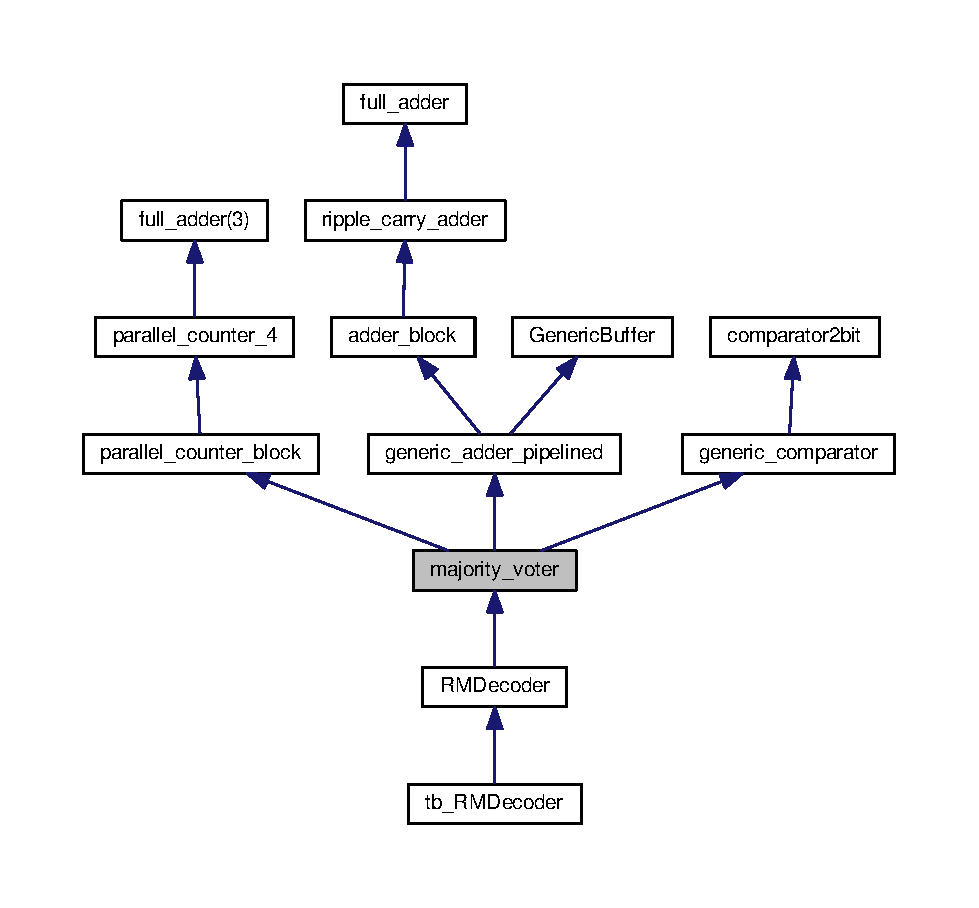
\includegraphics[width=350pt]{classmajority__voter__inherit__graph}
\end{center}
\end{figure}


Diagramma di collaborazione per majority\+\_\+voter\+:\nopagebreak
\begin{figure}[H]
\begin{center}
\leavevmode
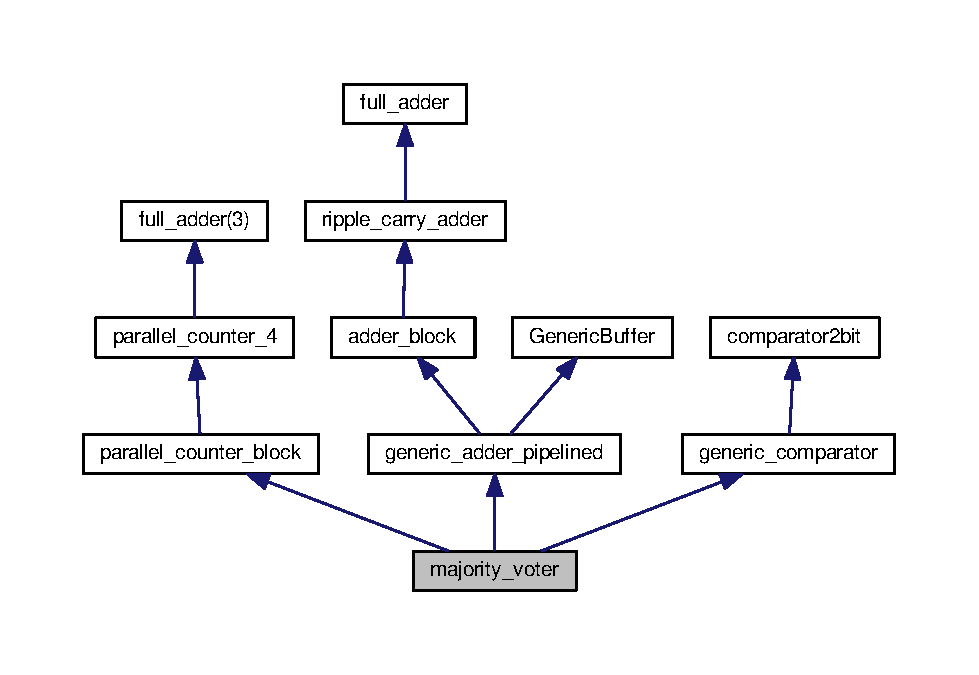
\includegraphics[width=350pt]{classmajority__voter__coll__graph}
\end{center}
\end{figure}
\subsection*{Entities}
\begin{DoxyCompactItemize}
\item 
\hyperlink{classmajority__voter_1_1_structural}{Structural} architecture
\end{DoxyCompactItemize}
\subsection*{Libraries}
 \begin{DoxyCompactItemize}
\item 
\hypertarget{classmajority__voter_gae4f03c286607f3181e16b9aa12d0c6d4}{\hyperlink{group___majority_voter_gae4f03c286607f3181e16b9aa12d0c6d4}{I\+E\+E\+E} }\label{classmajority__voter_gae4f03c286607f3181e16b9aa12d0c6d4}

\end{DoxyCompactItemize}
\subsection*{Use Clauses}
 \begin{DoxyCompactItemize}
\item 
\hypertarget{classmajority__voter_gaa4b2b25246a821511120e3149b003563}{\hyperlink{group___majority_voter_gaa4b2b25246a821511120e3149b003563}{S\+T\+D\+\_\+\+L\+O\+G\+I\+C\+\_\+1164}   }\label{classmajority__voter_gaa4b2b25246a821511120e3149b003563}

\item 
\hypertarget{classmajority__voter_gae00f3f04545af57582ff10609eee23e2}{\hyperlink{group___majority_voter_gae00f3f04545af57582ff10609eee23e2}{N\+U\+M\+E\+R\+I\+C\+\_\+\+S\+T\+D}   }\label{classmajority__voter_gae00f3f04545af57582ff10609eee23e2}

\item 
\hypertarget{classmajority__voter_ga6af860958a1bb510ee63ced87b57e11a}{\hyperlink{group___majority_voter_ga6af860958a1bb510ee63ced87b57e11a}{M\+A\+T\+H\+\_\+\+R\+E\+A\+L}   }\label{classmajority__voter_ga6af860958a1bb510ee63ced87b57e11a}

\end{DoxyCompactItemize}
\subsection*{Generics}
 \begin{DoxyCompactItemize}
\item 
\hypertarget{classmajority__voter_ga1f4ffccc38a894827f97741ab3077ef2}{\hyperlink{group___majority_voter_ga1f4ffccc38a894827f97741ab3077ef2}{width} {\bfseries {\bfseries \textcolor{vhdlchar}{N\+A\+T\+U\+R\+A\+L}\textcolor{vhdlchar}{ }\textcolor{vhdlchar}{ }\textcolor{vhdlchar}{\+:}\textcolor{vhdlchar}{=}\textcolor{vhdlchar}{ }\textcolor{vhdlchar}{ } \textcolor{vhdldigit}{64} \textcolor{vhdlchar}{ }}}}\label{classmajority__voter_ga1f4ffccc38a894827f97741ab3077ef2}

\end{DoxyCompactItemize}
\subsection*{Ports}
 \begin{DoxyCompactItemize}
\item 
\hypertarget{classmajority__voter_ga6231b307b7958b6060563aa2a93d345a}{\hyperlink{group___majority_voter_ga6231b307b7958b6060563aa2a93d345a}{clk}  {\bfseries {\bfseries \textcolor{vhdlchar}{in}\textcolor{vhdlchar}{ }}} {\bfseries \textcolor{vhdlchar}{S\+T\+D\+\_\+\+L\+O\+G\+I\+C}\textcolor{vhdlchar}{ }} }\label{classmajority__voter_ga6231b307b7958b6060563aa2a93d345a}

\item 
\hypertarget{classmajority__voter_ga8881084de0fcf748e41bd0fd1028445e}{\hyperlink{group___majority_voter_ga8881084de0fcf748e41bd0fd1028445e}{reset\+\_\+n}  {\bfseries {\bfseries \textcolor{vhdlchar}{in}\textcolor{vhdlchar}{ }}} {\bfseries \textcolor{vhdlchar}{S\+T\+D\+\_\+\+L\+O\+G\+I\+C}\textcolor{vhdlchar}{ }} }\label{classmajority__voter_ga8881084de0fcf748e41bd0fd1028445e}

\item 
\hypertarget{classmajority__voter_gaafe8d8f538bf4e2bdb9b8a73b793dad7}{\hyperlink{group___majority_voter_gaafe8d8f538bf4e2bdb9b8a73b793dad7}{data\+\_\+in}  {\bfseries {\bfseries \textcolor{vhdlchar}{in}\textcolor{vhdlchar}{ }}} {\bfseries \textcolor{vhdlchar}{S\+T\+D\+\_\+\+L\+O\+G\+I\+C\+\_\+\+V\+E\+C\+T\+O\+R}\textcolor{vhdlchar}{ }\textcolor{vhdlchar}{(}\textcolor{vhdlchar}{ }\textcolor{vhdlchar}{ }\textcolor{vhdlchar}{ }\textcolor{vhdlchar}{ }\textcolor{vhdlchar}{width}\textcolor{vhdlchar}{-\/}\textcolor{vhdlchar}{ } \textcolor{vhdldigit}{1} \textcolor{vhdlchar}{ }\textcolor{vhdlchar}{downto}\textcolor{vhdlchar}{ }\textcolor{vhdlchar}{ } \textcolor{vhdldigit}{0} \textcolor{vhdlchar}{ }\textcolor{vhdlchar}{)}\textcolor{vhdlchar}{ }} }\label{classmajority__voter_gaafe8d8f538bf4e2bdb9b8a73b793dad7}

\item 
\hypertarget{classmajority__voter_ga172bddca6a16c705b70242573b2df8e9}{\hyperlink{group___majority_voter_ga172bddca6a16c705b70242573b2df8e9}{majority}  {\bfseries {\bfseries \textcolor{vhdlchar}{out}\textcolor{vhdlchar}{ }}} {\bfseries \textcolor{vhdlchar}{S\+T\+D\+\_\+\+L\+O\+G\+I\+C}\textcolor{vhdlchar}{ }} }\label{classmajority__voter_ga172bddca6a16c705b70242573b2df8e9}

\end{DoxyCompactItemize}


\subsection{Descrizione dettagliata}
Implementazione V\+H\+D\+L \hyperlink{classmajority__voter_1_1_structural}{Structural} del majority voter. 


\begin{DoxyParams}{Parametri}
{\em width\mbox{[}in\mbox{]}} & parametro che determina la dimensione dell'input del componente, width $>$= 4\\
\hline
{\em clk\mbox{[}in\mbox{]}} & segnale di clock \\
\hline
{\em reset\+\_\+n\mbox{[}in\mbox{]}} & segnale di reset asincrono, attivo basso \\
\hline
{\em data\+\_\+in\mbox{[}in\mbox{]}} & stringa di bit di input su cui il componente lavora \\
\hline
{\em majority\mbox{[}out\mbox{]}} & bit di uscita \+: majority = \char`\"{}0\char`\"{} =$>$ nella stringa di input \#bit = 1 $>$= \#bit = 0 majority = \char`\"{}1\char`\"{} =$>$ nella stringa di input \#bit = 1 $>$ \#bit = 0 \\
\hline
\end{DoxyParams}


La documentazione per questa classe è stata generata a partire dal seguente file\+:\begin{DoxyCompactItemize}
\item 
R\+M\+Decoder/\+Majority\+Voter/\hyperlink{majority__voter_8vhd}{majority\+\_\+voter.\+vhd}\end{DoxyCompactItemize}

\hypertarget{classparallel__counter__4}{\section{parallel\+\_\+counter\+\_\+4 Entity Reference}
\label{classparallel__counter__4}\index{parallel\+\_\+counter\+\_\+4@{parallel\+\_\+counter\+\_\+4}}
}


Diagramma delle classi per parallel\+\_\+counter\+\_\+4\nopagebreak
\begin{figure}[H]
\begin{center}
\leavevmode
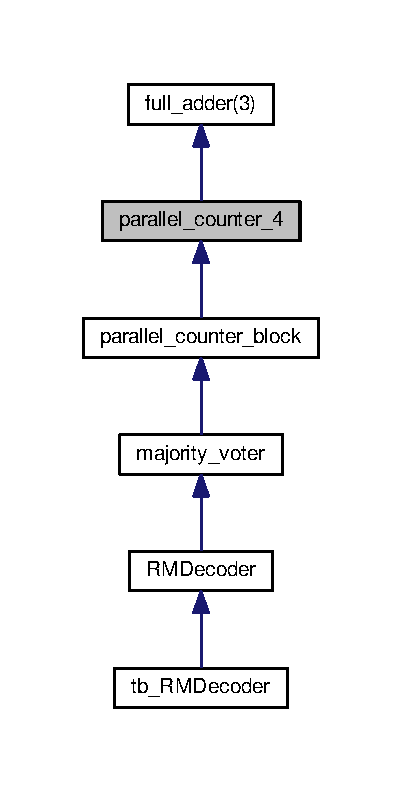
\includegraphics[width=193pt]{classparallel__counter__4__inherit__graph}
\end{center}
\end{figure}


Diagramma di collaborazione per parallel\+\_\+counter\+\_\+4\+:\nopagebreak
\begin{figure}[H]
\begin{center}
\leavevmode
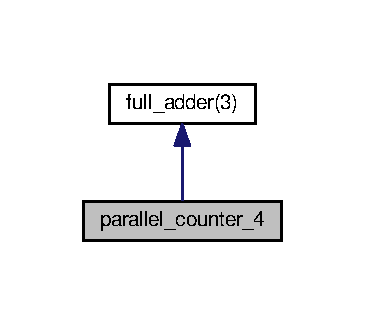
\includegraphics[width=175pt]{classparallel__counter__4__coll__graph}
\end{center}
\end{figure}
\subsection*{Entities}
\begin{DoxyCompactItemize}
\item 
\hyperlink{classparallel__counter__4_1_1_structural}{Structural} architecture
\end{DoxyCompactItemize}
\subsection*{Libraries}
 \begin{DoxyCompactItemize}
\item 
\hypertarget{classparallel__counter__4_gae4f03c286607f3181e16b9aa12d0c6d4}{\hyperlink{group___majority_voter_gae4f03c286607f3181e16b9aa12d0c6d4}{I\+E\+E\+E} }\label{classparallel__counter__4_gae4f03c286607f3181e16b9aa12d0c6d4}

\end{DoxyCompactItemize}
\subsection*{Use Clauses}
 \begin{DoxyCompactItemize}
\item 
\hypertarget{classparallel__counter__4_gaa4b2b25246a821511120e3149b003563}{\hyperlink{group___majority_voter_gaa4b2b25246a821511120e3149b003563}{S\+T\+D\+\_\+\+L\+O\+G\+I\+C\+\_\+1164}   }\label{classparallel__counter__4_gaa4b2b25246a821511120e3149b003563}

\end{DoxyCompactItemize}
\subsection*{Ports}
 \begin{DoxyCompactItemize}
\item 
\hypertarget{classparallel__counter__4_gad166bdfb934fb9b5f9d934bc77e58e21}{\hyperlink{group___majority_voter_gad166bdfb934fb9b5f9d934bc77e58e21}{X}  {\bfseries {\bfseries \textcolor{vhdlchar}{in}\textcolor{vhdlchar}{ }}} {\bfseries \textcolor{vhdlchar}{S\+T\+D\+\_\+\+L\+O\+G\+I\+C\+\_\+\+V\+E\+C\+T\+O\+R}\textcolor{vhdlchar}{ }\textcolor{vhdlchar}{(}\textcolor{vhdlchar}{ }\textcolor{vhdlchar}{ } \textcolor{vhdldigit}{3} \textcolor{vhdlchar}{ }\textcolor{vhdlchar}{downto}\textcolor{vhdlchar}{ }\textcolor{vhdlchar}{ } \textcolor{vhdldigit}{0} \textcolor{vhdlchar}{ }\textcolor{vhdlchar}{)}\textcolor{vhdlchar}{ }} }\label{classparallel__counter__4_gad166bdfb934fb9b5f9d934bc77e58e21}

\item 
\hypertarget{classparallel__counter__4_ga6f34466d04aa5a2a4a3313b99753df61}{\hyperlink{group___majority_voter_ga6f34466d04aa5a2a4a3313b99753df61}{C0}  {\bfseries {\bfseries \textcolor{vhdlchar}{out}\textcolor{vhdlchar}{ }}} {\bfseries \textcolor{vhdlchar}{S\+T\+D\+\_\+\+L\+O\+G\+I\+C}\textcolor{vhdlchar}{ }} }\label{classparallel__counter__4_ga6f34466d04aa5a2a4a3313b99753df61}

\item 
\hypertarget{classparallel__counter__4_gaf3a15fc1c76ca3d55f4c8d227d190085}{\hyperlink{group___majority_voter_gaf3a15fc1c76ca3d55f4c8d227d190085}{C1}  {\bfseries {\bfseries \textcolor{vhdlchar}{out}\textcolor{vhdlchar}{ }}} {\bfseries \textcolor{vhdlchar}{S\+T\+D\+\_\+\+L\+O\+G\+I\+C}\textcolor{vhdlchar}{ }} }\label{classparallel__counter__4_gaf3a15fc1c76ca3d55f4c8d227d190085}

\item 
\hypertarget{classparallel__counter__4_gafcc18913336fb764fc05b7d7e4753946}{\hyperlink{group___majority_voter_gafcc18913336fb764fc05b7d7e4753946}{C2}  {\bfseries {\bfseries \textcolor{vhdlchar}{out}\textcolor{vhdlchar}{ }}} {\bfseries \textcolor{vhdlchar}{S\+T\+D\+\_\+\+L\+O\+G\+I\+C}\textcolor{vhdlchar}{ }} }\label{classparallel__counter__4_gafcc18913336fb764fc05b7d7e4753946}

\end{DoxyCompactItemize}


La documentazione per questa classe è stata generata a partire dal seguente file\+:\begin{DoxyCompactItemize}
\item 
R\+M\+Decoder/\+Majority\+Voter/\hyperlink{parallel__counter__4_8vhd}{parallel\+\_\+counter\+\_\+4.\+vhd}\end{DoxyCompactItemize}

\hypertarget{classparallel__counter__block}{\section{parallel\+\_\+counter\+\_\+block Entity Reference}
\label{classparallel__counter__block}\index{parallel\+\_\+counter\+\_\+block@{parallel\+\_\+counter\+\_\+block}}
}


Implementazione V\+H\+D\+L \hyperlink{classparallel__counter__block_1_1_structural}{Structural} del Modulo 1 \+: genera width/4 contatori paralleli a 4 bit. Data una stringa di input di width bit, multipla di 4, assegna a ogni contatore un nibble. Ogni contatore parallelo a 4 bit codifica in binario il numero di 1 presente nel nibble di competenza.  




Diagramma delle classi per parallel\+\_\+counter\+\_\+block\nopagebreak
\begin{figure}[H]
\begin{center}
\leavevmode
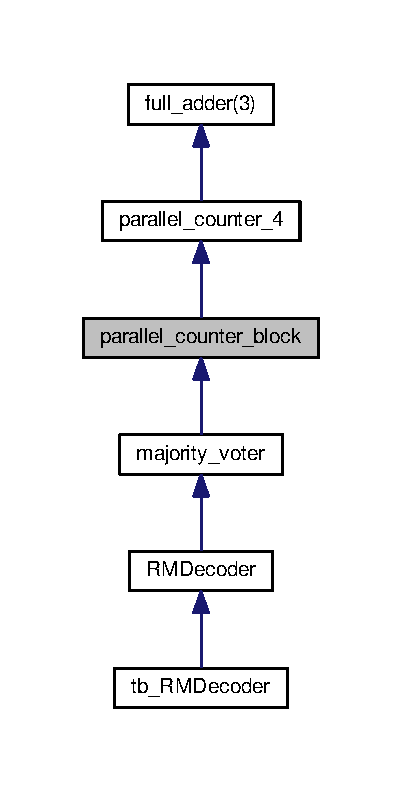
\includegraphics[width=193pt]{classparallel__counter__block__inherit__graph}
\end{center}
\end{figure}


Diagramma di collaborazione per parallel\+\_\+counter\+\_\+block\+:\nopagebreak
\begin{figure}[H]
\begin{center}
\leavevmode
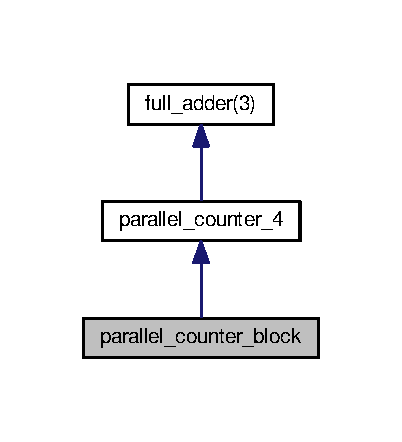
\includegraphics[width=193pt]{classparallel__counter__block__coll__graph}
\end{center}
\end{figure}
\subsection*{Entities}
\begin{DoxyCompactItemize}
\item 
\hyperlink{classparallel__counter__block_1_1_structural}{Structural} architecture
\end{DoxyCompactItemize}
\subsection*{Libraries}
 \begin{DoxyCompactItemize}
\item 
\hypertarget{classparallel__counter__block_gae4f03c286607f3181e16b9aa12d0c6d4}{\hyperlink{group___majority_voter_gae4f03c286607f3181e16b9aa12d0c6d4}{I\+E\+E\+E} }\label{classparallel__counter__block_gae4f03c286607f3181e16b9aa12d0c6d4}

\end{DoxyCompactItemize}
\subsection*{Use Clauses}
 \begin{DoxyCompactItemize}
\item 
\hypertarget{classparallel__counter__block_gaa4b2b25246a821511120e3149b003563}{\hyperlink{group___majority_voter_gaa4b2b25246a821511120e3149b003563}{S\+T\+D\+\_\+\+L\+O\+G\+I\+C\+\_\+1164}   }\label{classparallel__counter__block_gaa4b2b25246a821511120e3149b003563}

\end{DoxyCompactItemize}
\subsection*{Generics}
 \begin{DoxyCompactItemize}
\item 
\hypertarget{classparallel__counter__block_ga93ec5006d2e0a77a21f35a7e3c1ca827}{\hyperlink{group___majority_voter_ga93ec5006d2e0a77a21f35a7e3c1ca827}{width} {\bfseries {\bfseries \textcolor{vhdlchar}{N\+A\+T\+U\+R\+A\+L}\textcolor{vhdlchar}{ }\textcolor{vhdlchar}{ }\textcolor{vhdlchar}{\+:}\textcolor{vhdlchar}{=}\textcolor{vhdlchar}{ }\textcolor{vhdlchar}{ } \textcolor{vhdldigit}{8} \textcolor{vhdlchar}{ }}}}\label{classparallel__counter__block_ga93ec5006d2e0a77a21f35a7e3c1ca827}

\end{DoxyCompactItemize}
\subsection*{Ports}
 \begin{DoxyCompactItemize}
\item 
\hypertarget{classparallel__counter__block_gaafe8d8f538bf4e2bdb9b8a73b793dad7}{\hyperlink{group___majority_voter_gaafe8d8f538bf4e2bdb9b8a73b793dad7}{data\+\_\+in}  {\bfseries {\bfseries \textcolor{vhdlchar}{in}\textcolor{vhdlchar}{ }}} {\bfseries \textcolor{vhdlchar}{S\+T\+D\+\_\+\+L\+O\+G\+I\+C\+\_\+\+V\+E\+C\+T\+O\+R}\textcolor{vhdlchar}{ }\textcolor{vhdlchar}{(}\textcolor{vhdlchar}{ }\textcolor{vhdlchar}{ }\textcolor{vhdlchar}{ }\textcolor{vhdlchar}{ }\textcolor{vhdlchar}{width}\textcolor{vhdlchar}{-\/}\textcolor{vhdlchar}{ } \textcolor{vhdldigit}{1} \textcolor{vhdlchar}{ }\textcolor{vhdlchar}{downto}\textcolor{vhdlchar}{ }\textcolor{vhdlchar}{ } \textcolor{vhdldigit}{0} \textcolor{vhdlchar}{ }\textcolor{vhdlchar}{)}\textcolor{vhdlchar}{ }} }\label{classparallel__counter__block_gaafe8d8f538bf4e2bdb9b8a73b793dad7}

\item 
\hypertarget{classparallel__counter__block_ga2eb4ff23a26a8055101d64caa36f16ed}{\hyperlink{group___majority_voter_ga2eb4ff23a26a8055101d64caa36f16ed}{data\+\_\+out}  {\bfseries {\bfseries \textcolor{vhdlchar}{out}\textcolor{vhdlchar}{ }}} {\bfseries \textcolor{vhdlchar}{S\+T\+D\+\_\+\+L\+O\+G\+I\+C\+\_\+\+V\+E\+C\+T\+O\+R}\textcolor{vhdlchar}{ }\textcolor{vhdlchar}{(}\textcolor{vhdlchar}{ }\textcolor{vhdlchar}{(}\textcolor{vhdlchar}{ }\textcolor{vhdlchar}{ }\textcolor{vhdlchar}{ }\textcolor{vhdlchar}{ }\textcolor{vhdlchar}{width}\textcolor{vhdlchar}{-\/}\textcolor{vhdlchar}{ }\textcolor{vhdlchar}{(}\textcolor{vhdlchar}{ }\textcolor{vhdlchar}{ }\textcolor{vhdlchar}{ }\textcolor{vhdlchar}{ }\textcolor{vhdlchar}{width}\textcolor{vhdlchar}{/}\textcolor{vhdlchar}{ } \textcolor{vhdldigit}{4} \textcolor{vhdlchar}{ }\textcolor{vhdlchar}{)}\textcolor{vhdlchar}{ }\textcolor{vhdlchar}{)}\textcolor{vhdlchar}{ }\textcolor{vhdlchar}{-\/}\textcolor{vhdlchar}{ } \textcolor{vhdldigit}{1} \textcolor{vhdlchar}{ }\textcolor{vhdlchar}{downto}\textcolor{vhdlchar}{ }\textcolor{vhdlchar}{ } \textcolor{vhdldigit}{0} \textcolor{vhdlchar}{ }\textcolor{vhdlchar}{)}\textcolor{vhdlchar}{ }} }\label{classparallel__counter__block_ga2eb4ff23a26a8055101d64caa36f16ed}

\end{DoxyCompactItemize}


\subsection{Descrizione dettagliata}
Implementazione V\+H\+D\+L \hyperlink{classparallel__counter__block_1_1_structural}{Structural} del Modulo 1 \+: genera width/4 contatori paralleli a 4 bit. Data una stringa di input di width bit, multipla di 4, assegna a ogni contatore un nibble. Ogni contatore parallelo a 4 bit codifica in binario il numero di 1 presente nel nibble di competenza. 


\begin{DoxyParams}{Parametri}
{\em width\mbox{[}in\mbox{]}} & parametro che determina la dimensione dell'input del componente, width multiplo di 4\\
\hline
{\em data\+\_\+in\mbox{[}in\mbox{]}} & stringa di bit di input di dimensione width su cui il componente lavora \\
\hline
{\em data\+\_\+out\mbox{[}out\mbox{]}} & stringa di bit di uscita di dimensione width-\/(width/4) che è la concatenazione degli output dei singoli contatori paralleli a 4 bit =$>$ concatenzaione di stringhe da 3 bit. \\
\hline
\end{DoxyParams}


La documentazione per questa classe è stata generata a partire dal seguente file\+:\begin{DoxyCompactItemize}
\item 
R\+M\+Decoder/\+Majority\+Voter/\hyperlink{parallel__counter__block_8vhd}{parallel\+\_\+counter\+\_\+block.\+vhd}\end{DoxyCompactItemize}

\hypertarget{classripple__carry__adder}{\section{ripple\+\_\+carry\+\_\+adder Entity Reference}
\label{classripple__carry__adder}\index{ripple\+\_\+carry\+\_\+adder@{ripple\+\_\+carry\+\_\+adder}}
}


Implementazione V\+H\+D\+L Structural di un Ripple Carry Adder generico a N bit.  




Diagramma delle classi per ripple\+\_\+carry\+\_\+adder\nopagebreak
\begin{figure}[H]
\begin{center}
\leavevmode
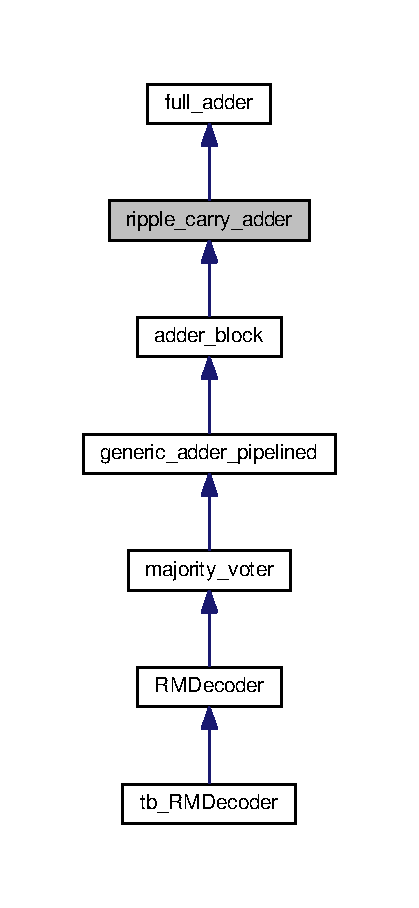
\includegraphics[width=201pt]{classripple__carry__adder__inherit__graph}
\end{center}
\end{figure}


Diagramma di collaborazione per ripple\+\_\+carry\+\_\+adder\+:\nopagebreak
\begin{figure}[H]
\begin{center}
\leavevmode
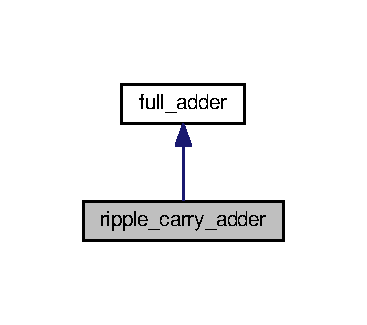
\includegraphics[width=176pt]{classripple__carry__adder__coll__graph}
\end{center}
\end{figure}
\subsection*{Entities}
\begin{DoxyCompactItemize}
\item 
\hyperlink{classripple__carry__adder_1_1structural}{structural} architecture
\end{DoxyCompactItemize}
\subsection*{Libraries}
 \begin{DoxyCompactItemize}
\item 
\hypertarget{classripple__carry__adder_gae4f03c286607f3181e16b9aa12d0c6d4}{\hyperlink{group___majority_voter_gae4f03c286607f3181e16b9aa12d0c6d4}{I\+E\+E\+E} }\label{classripple__carry__adder_gae4f03c286607f3181e16b9aa12d0c6d4}

\end{DoxyCompactItemize}
\subsection*{Use Clauses}
 \begin{DoxyCompactItemize}
\item 
\hypertarget{classripple__carry__adder_gaa4b2b25246a821511120e3149b003563}{\hyperlink{group___majority_voter_gaa4b2b25246a821511120e3149b003563}{S\+T\+D\+\_\+\+L\+O\+G\+I\+C\+\_\+1164}   }\label{classripple__carry__adder_gaa4b2b25246a821511120e3149b003563}

\end{DoxyCompactItemize}
\subsection*{Generics}
 \begin{DoxyCompactItemize}
\item 
\hypertarget{classripple__carry__adder_ga618671bc4830b9ddb3181ac86d119b6b}{\hyperlink{group___majority_voter_ga618671bc4830b9ddb3181ac86d119b6b}{N} {\bfseries {\bfseries \textcolor{vhdlchar}{natural}\textcolor{vhdlchar}{ }\textcolor{vhdlchar}{ }\textcolor{vhdlchar}{\+:}\textcolor{vhdlchar}{=}\textcolor{vhdlchar}{ }\textcolor{vhdlchar}{ } \textcolor{vhdldigit}{4} \textcolor{vhdlchar}{ }}}}\label{classripple__carry__adder_ga618671bc4830b9ddb3181ac86d119b6b}

\end{DoxyCompactItemize}
\subsection*{Ports}
 \begin{DoxyCompactItemize}
\item 
\hypertarget{classripple__carry__adder_ga45c8fb904508ebf47bf8113b52bab3b2}{\hyperlink{group___majority_voter_ga45c8fb904508ebf47bf8113b52bab3b2}{x}  {\bfseries {\bfseries \textcolor{vhdlchar}{in}\textcolor{vhdlchar}{ }}} {\bfseries \textcolor{vhdlchar}{S\+T\+D\+\_\+\+L\+O\+G\+I\+C\+\_\+\+V\+E\+C\+T\+O\+R}\textcolor{vhdlchar}{ }\textcolor{vhdlchar}{(}\textcolor{vhdlchar}{ }\textcolor{vhdlchar}{ }\textcolor{vhdlchar}{ }\textcolor{vhdlchar}{ }\textcolor{vhdlchar}{N}\textcolor{vhdlchar}{-\/}\textcolor{vhdlchar}{ } \textcolor{vhdldigit}{1} \textcolor{vhdlchar}{ }\textcolor{vhdlchar}{downto}\textcolor{vhdlchar}{ }\textcolor{vhdlchar}{ } \textcolor{vhdldigit}{0} \textcolor{vhdlchar}{ }\textcolor{vhdlchar}{)}\textcolor{vhdlchar}{ }} }\label{classripple__carry__adder_ga45c8fb904508ebf47bf8113b52bab3b2}

\item 
\hypertarget{classripple__carry__adder_ga580c4107150f1a8ce9f0f25fcbb33f08}{\hyperlink{group___majority_voter_ga580c4107150f1a8ce9f0f25fcbb33f08}{y}  {\bfseries {\bfseries \textcolor{vhdlchar}{in}\textcolor{vhdlchar}{ }}} {\bfseries \textcolor{vhdlchar}{S\+T\+D\+\_\+\+L\+O\+G\+I\+C\+\_\+\+V\+E\+C\+T\+O\+R}\textcolor{vhdlchar}{ }\textcolor{vhdlchar}{(}\textcolor{vhdlchar}{ }\textcolor{vhdlchar}{ }\textcolor{vhdlchar}{ }\textcolor{vhdlchar}{ }\textcolor{vhdlchar}{N}\textcolor{vhdlchar}{-\/}\textcolor{vhdlchar}{ } \textcolor{vhdldigit}{1} \textcolor{vhdlchar}{ }\textcolor{vhdlchar}{downto}\textcolor{vhdlchar}{ }\textcolor{vhdlchar}{ } \textcolor{vhdldigit}{0} \textcolor{vhdlchar}{ }\textcolor{vhdlchar}{)}\textcolor{vhdlchar}{ }} }\label{classripple__carry__adder_ga580c4107150f1a8ce9f0f25fcbb33f08}

\item 
\hypertarget{classripple__carry__adder_gab93e0e530f7cfe8f44daa9285209cca1}{\hyperlink{group___majority_voter_gab93e0e530f7cfe8f44daa9285209cca1}{carry\+\_\+in}  {\bfseries {\bfseries \textcolor{vhdlchar}{in}\textcolor{vhdlchar}{ }}} {\bfseries \textcolor{vhdlchar}{S\+T\+D\+\_\+\+L\+O\+G\+I\+C}\textcolor{vhdlchar}{ }} }\label{classripple__carry__adder_gab93e0e530f7cfe8f44daa9285209cca1}

\item 
\hypertarget{classripple__carry__adder_gafcc7c006376592bcf77bccdcfd0a99bc}{\hyperlink{group___majority_voter_gafcc7c006376592bcf77bccdcfd0a99bc}{carry\+\_\+out}  {\bfseries {\bfseries \textcolor{vhdlchar}{out}\textcolor{vhdlchar}{ }}} {\bfseries \textcolor{vhdlchar}{S\+T\+D\+\_\+\+L\+O\+G\+I\+C}\textcolor{vhdlchar}{ }} }\label{classripple__carry__adder_gafcc7c006376592bcf77bccdcfd0a99bc}

\item 
\hypertarget{classripple__carry__adder_ga1e89beb6ed04c1a4951aeb8c68b5cca3}{\hyperlink{group___majority_voter_ga1e89beb6ed04c1a4951aeb8c68b5cca3}{sum}  {\bfseries {\bfseries \textcolor{vhdlchar}{out}\textcolor{vhdlchar}{ }}} {\bfseries \textcolor{vhdlchar}{S\+T\+D\+\_\+\+L\+O\+G\+I\+C\+\_\+\+V\+E\+C\+T\+O\+R}\textcolor{vhdlchar}{ }\textcolor{vhdlchar}{(}\textcolor{vhdlchar}{ }\textcolor{vhdlchar}{ }\textcolor{vhdlchar}{ }\textcolor{vhdlchar}{ }\textcolor{vhdlchar}{N}\textcolor{vhdlchar}{-\/}\textcolor{vhdlchar}{ } \textcolor{vhdldigit}{1} \textcolor{vhdlchar}{ }\textcolor{vhdlchar}{downto}\textcolor{vhdlchar}{ }\textcolor{vhdlchar}{ } \textcolor{vhdldigit}{0} \textcolor{vhdlchar}{ }\textcolor{vhdlchar}{)}\textcolor{vhdlchar}{ }} }\label{classripple__carry__adder_ga1e89beb6ed04c1a4951aeb8c68b5cca3}

\end{DoxyCompactItemize}


\subsection{Descrizione dettagliata}
Implementazione V\+H\+D\+L Structural di un Ripple Carry Adder generico a N bit. 


\begin{DoxyParams}{Parametri}
{\em N\mbox{[}in\mbox{]}} & parametro che determina il numero di bit per addendo\\
\hline
{\em x\mbox{[}in\mbox{]}} & addendo 1 \\
\hline
{\em x\mbox{[}in\mbox{]}} & addendo 2 \\
\hline
{\em carry\+\_\+in\mbox{[}in\mbox{]}} & carry in ingresso \\
\hline
{\em carry\+\_\+out\mbox{[}out\mbox{]}} & carry in uscita \\
\hline
{\em sum\mbox{[}out\mbox{]}} & somma dei due addendi \\
\hline
\end{DoxyParams}


La documentazione per questa classe è stata generata a partire dal seguente file\+:\begin{DoxyCompactItemize}
\item 
R\+M\+Decoder/\+Majority\+Voter/\hyperlink{ripple__carry__adder_8vhd}{ripple\+\_\+carry\+\_\+adder.\+vhd}\end{DoxyCompactItemize}

\hypertarget{class_r_m_decoder}{\section{R\+M\+Decoder Entity Reference}
\label{class_r_m_decoder}\index{R\+M\+Decoder@{R\+M\+Decoder}}
}


Implementazione V\+H\+D\+L del decodificatore per codici di Reed-\/\+Muller(1,m)  




Diagramma delle classi per R\+M\+Decoder\nopagebreak
\begin{figure}[H]
\begin{center}
\leavevmode
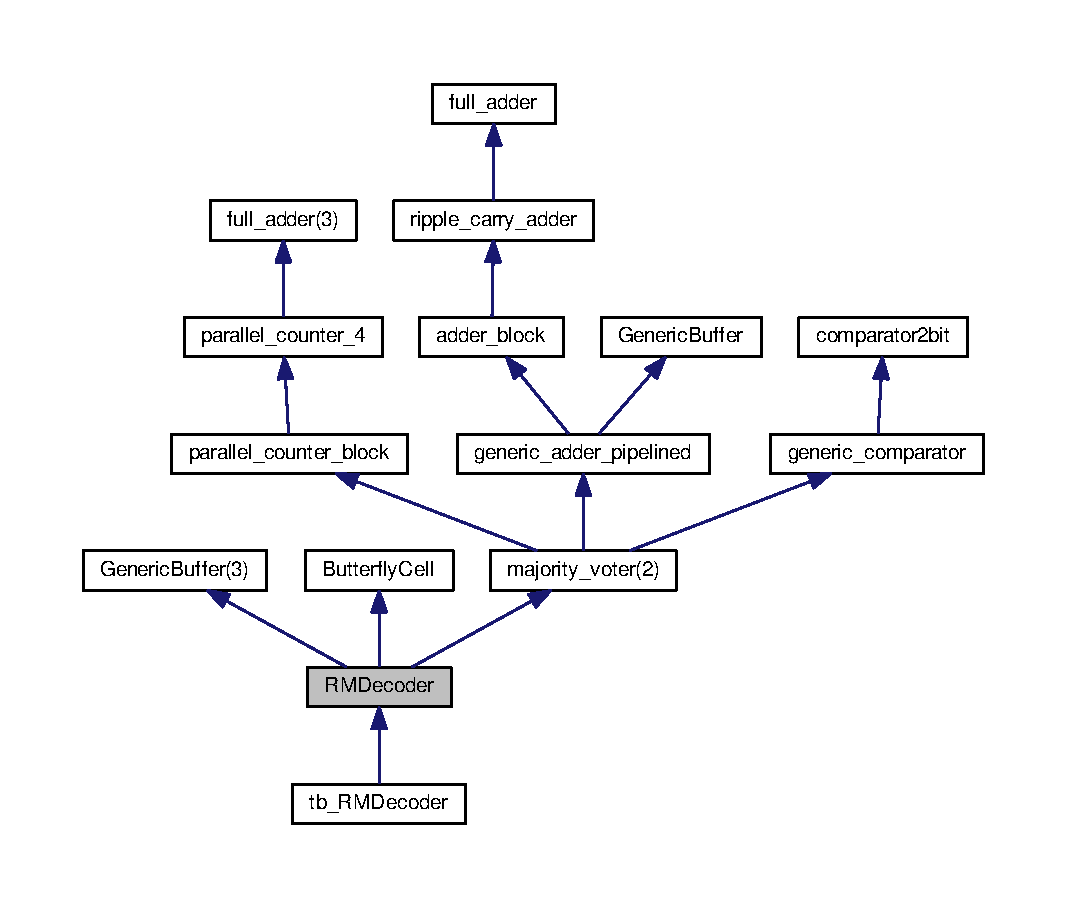
\includegraphics[width=350pt]{class_r_m_decoder__inherit__graph}
\end{center}
\end{figure}


Diagramma di collaborazione per R\+M\+Decoder\+:\nopagebreak
\begin{figure}[H]
\begin{center}
\leavevmode
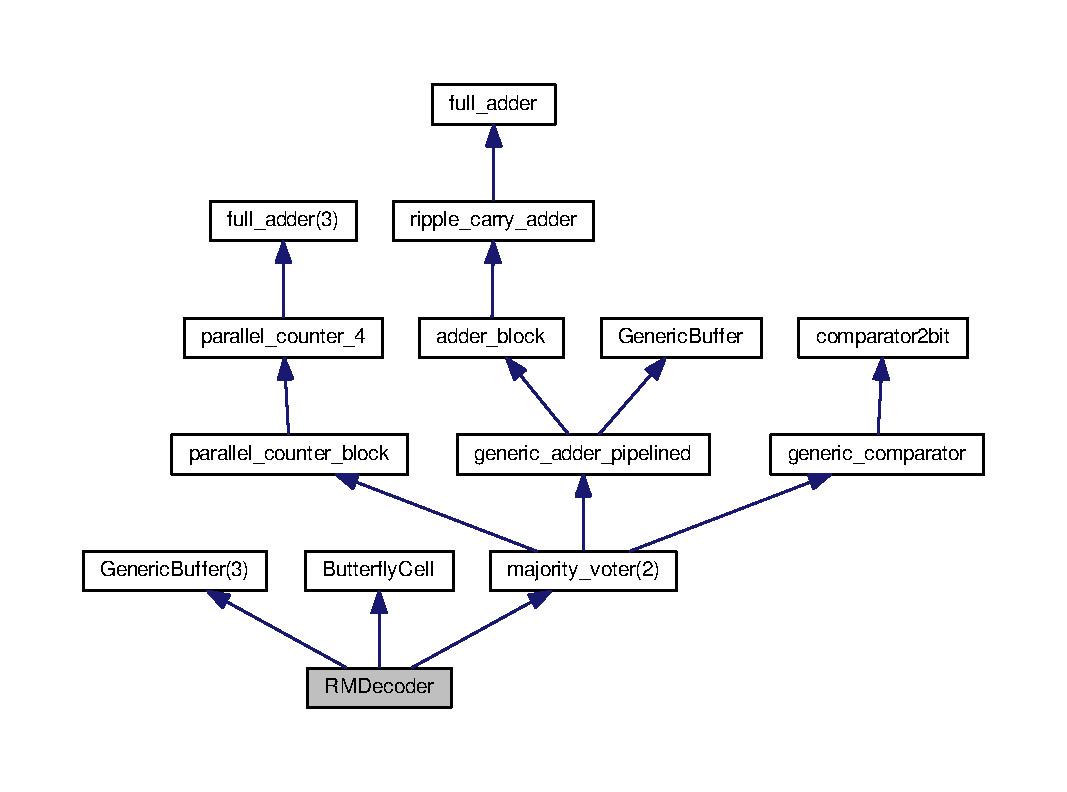
\includegraphics[width=350pt]{class_r_m_decoder__coll__graph}
\end{center}
\end{figure}
\subsection*{Entities}
\begin{DoxyCompactItemize}
\item 
\hyperlink{class_r_m_decoder_1_1_structural}{Structural} architecture
\end{DoxyCompactItemize}
\subsection*{Libraries}
 \begin{DoxyCompactItemize}
\item 
\hypertarget{class_r_m_decoder_ga0a6af6eef40212dbaf130d57ce711256}{\hyperlink{group___r_m_decoder_ga0a6af6eef40212dbaf130d57ce711256}{ieee} }\label{class_r_m_decoder_ga0a6af6eef40212dbaf130d57ce711256}

\end{DoxyCompactItemize}
\subsection*{Use Clauses}
 \begin{DoxyCompactItemize}
\item 
\hypertarget{class_r_m_decoder_gacd03516902501cd1c7296a98e22c6fcb}{\hyperlink{group___r_m_decoder_gacd03516902501cd1c7296a98e22c6fcb}{std\+\_\+logic\+\_\+1164}   }\label{class_r_m_decoder_gacd03516902501cd1c7296a98e22c6fcb}

\item 
\hypertarget{class_r_m_decoder_ga2edc34402b573437d5f25fa90ba4013e}{\hyperlink{group___r_m_decoder_ga2edc34402b573437d5f25fa90ba4013e}{numeric\+\_\+std}   }\label{class_r_m_decoder_ga2edc34402b573437d5f25fa90ba4013e}

\end{DoxyCompactItemize}
\subsection*{Generics}
 \begin{DoxyCompactItemize}
\item 
\hypertarget{class_r_m_decoder_gad4fc2116999466ec7397a88a6e28908b}{\hyperlink{group___r_m_decoder_gad4fc2116999466ec7397a88a6e28908b}{m} {\bfseries {\bfseries \textcolor{vhdlchar}{natural}\textcolor{vhdlchar}{ }\textcolor{vhdlchar}{ }\textcolor{vhdlchar}{\+:}\textcolor{vhdlchar}{=}\textcolor{vhdlchar}{ }\textcolor{vhdlchar}{ } \textcolor{vhdldigit}{6} \textcolor{vhdlchar}{ }}}}\label{class_r_m_decoder_gad4fc2116999466ec7397a88a6e28908b}

\item 
\hypertarget{class_r_m_decoder_gaa6a3bcd7caff4ed469a24b721a55d4f2}{\hyperlink{group___r_m_decoder_gaa6a3bcd7caff4ed469a24b721a55d4f2}{generator\+\_\+matrix\+\_\+01} {\bfseries {\bfseries \textcolor{vhdlchar}{boolean}\textcolor{vhdlchar}{ }\textcolor{vhdlchar}{ }\textcolor{vhdlchar}{\+:}\textcolor{vhdlchar}{=}\textcolor{vhdlchar}{ }\textcolor{vhdlchar}{ }\textcolor{vhdlchar}{ }\textcolor{vhdlchar}{ }\textcolor{vhdlchar}{true}\textcolor{vhdlchar}{ }}}}\label{class_r_m_decoder_gaa6a3bcd7caff4ed469a24b721a55d4f2}

\end{DoxyCompactItemize}
\subsection*{Ports}
 \begin{DoxyCompactItemize}
\item 
\hypertarget{class_r_m_decoder_gadfc2d5e995e9c6876b2e55bf6a5c4071}{\hyperlink{group___r_m_decoder_gadfc2d5e995e9c6876b2e55bf6a5c4071}{clock}  {\bfseries {\bfseries \textcolor{vhdlchar}{in}\textcolor{vhdlchar}{ }}} {\bfseries \textcolor{vhdlchar}{std\+\_\+logic}\textcolor{vhdlchar}{ }} }\label{class_r_m_decoder_gadfc2d5e995e9c6876b2e55bf6a5c4071}

\item 
\hypertarget{class_r_m_decoder_ga446ea52ed8c4a84181a47d9165ce41a5}{\hyperlink{group___r_m_decoder_ga446ea52ed8c4a84181a47d9165ce41a5}{reset\+\_\+n}  {\bfseries {\bfseries \textcolor{vhdlchar}{in}\textcolor{vhdlchar}{ }}} {\bfseries \textcolor{vhdlchar}{std\+\_\+logic}\textcolor{vhdlchar}{ }} }\label{class_r_m_decoder_ga446ea52ed8c4a84181a47d9165ce41a5}

\item 
\hypertarget{class_r_m_decoder_ga2b10c9545b143a051326b4159f5bb7e8}{\hyperlink{group___r_m_decoder_ga2b10c9545b143a051326b4159f5bb7e8}{data\+\_\+in}  {\bfseries {\bfseries \textcolor{vhdlchar}{in}\textcolor{vhdlchar}{ }}} {\bfseries \textcolor{vhdlchar}{std\+\_\+logic\+\_\+vector}\textcolor{vhdlchar}{ }\textcolor{vhdlchar}{(}\textcolor{vhdlchar}{ }\textcolor{vhdlchar}{ } \textcolor{vhdldigit}{2} \textcolor{vhdlchar}{$\ast$}\textcolor{vhdlchar}{$\ast$}\textcolor{vhdlchar}{ }\textcolor{vhdlchar}{ }\textcolor{vhdlchar}{ }\textcolor{vhdlchar}{m}\textcolor{vhdlchar}{-\/}\textcolor{vhdlchar}{ } \textcolor{vhdldigit}{1} \textcolor{vhdlchar}{ }\textcolor{vhdlchar}{downto}\textcolor{vhdlchar}{ }\textcolor{vhdlchar}{ } \textcolor{vhdldigit}{0} \textcolor{vhdlchar}{ }\textcolor{vhdlchar}{)}\textcolor{vhdlchar}{ }} }\label{class_r_m_decoder_ga2b10c9545b143a051326b4159f5bb7e8}

\item 
\hypertarget{class_r_m_decoder_ga5b228b0942e33af121e97ced334b88e5}{\hyperlink{group___r_m_decoder_ga5b228b0942e33af121e97ced334b88e5}{data\+\_\+out}  {\bfseries {\bfseries \textcolor{vhdlchar}{out}\textcolor{vhdlchar}{ }}} {\bfseries \textcolor{vhdlchar}{std\+\_\+logic\+\_\+vector}\textcolor{vhdlchar}{ }\textcolor{vhdlchar}{(}\textcolor{vhdlchar}{ }\textcolor{vhdlchar}{ }\textcolor{vhdlchar}{ }\textcolor{vhdlchar}{ }\textcolor{vhdlchar}{m}\textcolor{vhdlchar}{ }\textcolor{vhdlchar}{downto}\textcolor{vhdlchar}{ }\textcolor{vhdlchar}{ } \textcolor{vhdldigit}{0} \textcolor{vhdlchar}{ }\textcolor{vhdlchar}{)}\textcolor{vhdlchar}{ }} }\label{class_r_m_decoder_ga5b228b0942e33af121e97ced334b88e5}

\end{DoxyCompactItemize}


\subsection{Descrizione dettagliata}
Implementazione V\+H\+D\+L del decodificatore per codici di Reed-\/\+Muller(1,m) 

Tale implementazione fa uso della tecnica con majority-\/voter ed e' pipelined, con numero di stadi delle pipe variabile in base al particolare codice di Reed-\/\+Muller. Il numero totale di stadi della pipe, in funzione di \char`\"{}m\char`\"{}, e' 2m-\/4. Ad esempio, per codici R\+M(1,7), il numero di stadi della pipe e' 10. Il componente, in questo modo, manifesta, questo si, una latenza di 2m-\/4 colpi di clock, ma e' potenzialmente in grado di completare una decodifica per colpo di clock.~\newline
 Il seguente esempio istanzia un encoder ed un decoder. L'output dell'encoder viene posto in ingresso al decoder. L'input dell'encoder viene controllato attraverso un V\+I\+O. Lo stesso V\+I\+O viene usato anche per monitorare l'uscita dell'encoder e l'uscita del decoder, oltre che per controllare il segnale di reset di quest'ultimo.


\begin{DoxyCode}
1 encoder : \hyperlink{class_r_m_encoder}{RMEncoder}
2     \textcolor{keywordflow}{Generic} \textcolor{keywordflow}{map} (   m                   => m,
3                     generator\_matrix\_01  => generator\_matrix\_01\textcolor{vhdlchar}{)}
4     \textcolor{keywordflow}{Port} \textcolor{keywordflow}{map} (      data\_in              => encoder\_data\_in,
5                     data\_out             => encoder\_data\_out \textcolor{vhdlchar}{)};
6 
7 decoder : \hyperlink{class_r_m_decoder}{RMDecoder}
8     \textcolor{keywordflow}{Generic} \textcolor{keywordflow}{map} (   m                   => m,
9                     generator\_matrix\_01  => generator\_matrix\_01\textcolor{vhdlchar}{)}
10     \textcolor{keywordflow}{Port} \textcolor{keywordflow}{map} (      clock                => clock,
11                     reset\_n              => reset\_n,
12                     data\_in              => encoder\_data\_out ,
13                     data\_out             => decoder\_data\_out \textcolor{vhdlchar}{)};
14 
15 vio : vio\_0
16     \textcolor{keywordflow}{Port} \textcolor{keywordflow}{map} (  clk              => clock,
17                 probe\_in0        => encoder\_data\_out ,
18                 probe\_in1        => decoder\_data\_out ,
19                 probe\_out0       => encoder\_data\_in,
20                 probe\_out1\textcolor{vhdlchar}{(}\textcolor{vhdllogic}{0}\textcolor{vhdlchar}{)}    => reset\_n\textcolor{vhdlchar}{)};
\end{DoxyCode}


\begin{DoxyWarning}{Avvertimento}
I codici devono essere stati ottenuti con una matrice di generazione in forma canonica. Vedi il parametro generator\+\_\+matrix\+\_\+01.
\end{DoxyWarning}

\begin{DoxyParams}{Parametri}
{\em m\mbox{[}in\mbox{]}} & parametro \char`\"{}m\char`\"{} del codice di Reed-\/\+Muller; incide sulla dimensione, in bit, dell'input e dell' output del componente\+: l'input sara' 2$^\wedge$m bit, mentre l'output m+1 bit. Oltre che stabilire il particolare codice che e' possibile decifrare, incide sul numero di stadi della pipe di cui il decoder e' composto. Il numero totale di stadi della pipe, in funzione di \char`\"{}m\char`\"{}, e' 2(m-\/3)+1. Ad esempio, per codici R\+M(1,7), il numero di stadi e' 9. \\
\hline
{\em generator\+\_\+matrix\+\_\+01\mbox{[}in\mbox{]}} & permette di scegliere la matrice di generazione da usare in fase di decodifica. Scegliendo generator\+\_\+matrix\+\_\+01 =$>$ true, verra' usata una matrice~\newline
 1111111111111111~\newline
 0000000011111111~\newline
 0000111100001111~\newline
 0011001100110011~\newline
 0101010101010101~\newline
 Se, invece, generator\+\_\+matrix\+\_\+01 =$>$ false, verra' usata una matrice~\newline
 1111111111111111~\newline
 1111111100000000~\newline
 1111000011110000~\newline
 1100110011001100~\newline
 1010101010101010 \\
\hline
{\em clock\mbox{[}in\mbox{]}} & segnale di clock \\
\hline
{\em reset\+\_\+n\mbox{[}in\mbox{]}} & segnale di reset asincrono, attivo basso \\
\hline
{\em data\+\_\+in\mbox{[}in\mbox{]}} & codice di Reed-\/\+Muller R\+M(1, m) da decodificare, di lunghezza 2$^\wedge$\{m\} bit \\
\hline
{\em data\+\_\+out\mbox{[}out\mbox{]}} & stringa di bit corrispondente al codice di Reed-\/\+Muller R\+M(1, m) decodificato, di lunghezza pari ad m bit \\
\hline
\end{DoxyParams}
\begin{DoxyRefDesc}{Test}
\item[\hyperlink{test__test000001}{Test}]R\+M(1,m), m=3~\newline
 \end{DoxyRefDesc}
\begin{TabularC}{2}
\hline
\rowcolor{lightgray}{\bf data\+\_\+in}&{\bf data\+\_\+out }\\\cline{1-2}
x\char`\"{}00\char`\"{}&x\char`\"{}0\char`\"{} \\\cline{1-2}
x\char`\"{}55\char`\"{}&x\char`\"{}1\char`\"{} \\\cline{1-2}
x\char`\"{}33\char`\"{}&x\char`\"{}2\char`\"{} \\\cline{1-2}
x\char`\"{}66\char`\"{}&x\char`\"{}3\char`\"{} \\\cline{1-2}
x\char`\"{}0f\char`\"{}&x\char`\"{}4\char`\"{} \\\cline{1-2}
x\char`\"{}5a\char`\"{}&x\char`\"{}5\char`\"{} \\\cline{1-2}
x\char`\"{}3c\char`\"{}&x\char`\"{}6\char`\"{} \\\cline{1-2}
x\char`\"{}69\char`\"{}&x\char`\"{}7\char`\"{} \\\cline{1-2}
x\char`\"{}ff\char`\"{}&x\char`\"{}8\char`\"{} \\\cline{1-2}
x\char`\"{}aa\char`\"{}&x\char`\"{}9\char`\"{} \\\cline{1-2}
x\char`\"{}cc\char`\"{}&x\char`\"{}a\char`\"{} \\\cline{1-2}
x\char`\"{}99\char`\"{}&x\char`\"{}b\char`\"{} \\\cline{1-2}
x\char`\"{}f0\char`\"{}&x\char`\"{}c\char`\"{} \\\cline{1-2}
x\char`\"{}a5\char`\"{}&x\char`\"{}d\char`\"{} \\\cline{1-2}
x\char`\"{}c3\char`\"{}&x\char`\"{}e\char`\"{} \\\cline{1-2}
x\char`\"{}96\char`\"{}&x\char`\"{}f\char`\"{} \\\cline{1-2}
\end{TabularC}
R\+M(1,m), m=4~\newline
 \begin{TabularC}{2}
\hline
\rowcolor{lightgray}{\bf data\+\_\+in}&{\bf data\+\_\+out }\\\cline{1-2}
x\char`\"{}0000\char`\"{}&x\char`\"{}00\char`\"{} \\\cline{1-2}
x\char`\"{}5555\char`\"{}&x\char`\"{}01\char`\"{} \\\cline{1-2}
x\char`\"{}3333\char`\"{}&x\char`\"{}02\char`\"{} \\\cline{1-2}
x\char`\"{}6666\char`\"{}&x\char`\"{}03\char`\"{} \\\cline{1-2}
x\char`\"{}0f0f\char`\"{}&x\char`\"{}04\char`\"{} \\\cline{1-2}
x\char`\"{}5a5a\char`\"{}&x\char`\"{}05\char`\"{} \\\cline{1-2}
x\char`\"{}3c3c\char`\"{}&x\char`\"{}06\char`\"{} \\\cline{1-2}
x\char`\"{}6969\char`\"{}&x\char`\"{}07\char`\"{} \\\cline{1-2}
x\char`\"{}00ff\char`\"{}&x\char`\"{}08\char`\"{} \\\cline{1-2}
x\char`\"{}55aa\char`\"{}&x\char`\"{}09\char`\"{} \\\cline{1-2}
x\char`\"{}33cc\char`\"{}&x\char`\"{}0a\char`\"{} \\\cline{1-2}
x\char`\"{}6699\char`\"{}&x\char`\"{}0b\char`\"{} \\\cline{1-2}
x\char`\"{}0ff0\char`\"{}&x\char`\"{}0c\char`\"{} \\\cline{1-2}
x\char`\"{}5aa5\char`\"{}&x\char`\"{}0d\char`\"{} \\\cline{1-2}
x\char`\"{}3cc3\char`\"{}&x\char`\"{}0e\char`\"{} \\\cline{1-2}
x\char`\"{}6996\char`\"{}&x\char`\"{}0f\char`\"{} \\\cline{1-2}
x\char`\"{}ffff\char`\"{}&x\char`\"{}10\char`\"{} \\\cline{1-2}
x\char`\"{}aaaa\char`\"{}&x\char`\"{}11\char`\"{} \\\cline{1-2}
x\char`\"{}cccc\char`\"{}&x\char`\"{}12\char`\"{} \\\cline{1-2}
x\char`\"{}9999\char`\"{}&x\char`\"{}13\char`\"{} \\\cline{1-2}
x\char`\"{}f0f0\char`\"{}&x\char`\"{}14\char`\"{} \\\cline{1-2}
x\char`\"{}a5a5\char`\"{}&x\char`\"{}15\char`\"{} \\\cline{1-2}
x\char`\"{}c3c3\char`\"{}&x\char`\"{}16\char`\"{} \\\cline{1-2}
x\char`\"{}9696\char`\"{}&x\char`\"{}17\char`\"{} \\\cline{1-2}
x\char`\"{}ff00\char`\"{}&x\char`\"{}18\char`\"{} \\\cline{1-2}
x\char`\"{}aa55\char`\"{}&x\char`\"{}19\char`\"{} \\\cline{1-2}
x\char`\"{}cc33\char`\"{}&x\char`\"{}1a\char`\"{} \\\cline{1-2}
x\char`\"{}9966\char`\"{}&x\char`\"{}1b\char`\"{} \\\cline{1-2}
x\char`\"{}f00f\char`\"{}&x\char`\"{}1c\char`\"{} \\\cline{1-2}
x\char`\"{}a55a\char`\"{}&x\char`\"{}1d\char`\"{} \\\cline{1-2}
x\char`\"{}c33c\char`\"{}&x\char`\"{}1e\char`\"{} \\\cline{1-2}
x\char`\"{}9669\char`\"{}&x\char`\"{}1f\char`\"{} \\\cline{1-2}
\end{TabularC}


La documentazione per questa classe è stata generata a partire dal seguente file\+:\begin{DoxyCompactItemize}
\item 
R\+M\+Decoder/\hyperlink{_r_m_decoder_8vhd}{R\+M\+Decoder.\+vhd}\end{DoxyCompactItemize}

\hypertarget{class_r_m_encoder}{\section{R\+M\+Encoder Entity Reference}
\label{class_r_m_encoder}\index{R\+M\+Encoder@{R\+M\+Encoder}}
}


Implementazione V\+H\+D\+L del codificatore per codici di Reed-\/\+Muller(1,m)  




Diagramma delle classi per R\+M\+Encoder\nopagebreak
\begin{figure}[H]
\begin{center}
\leavevmode
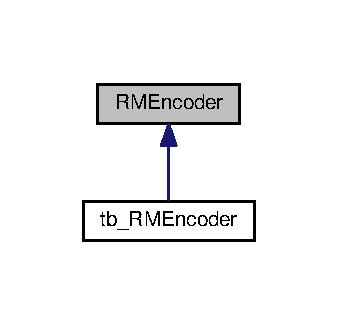
\includegraphics[width=162pt]{class_r_m_encoder__inherit__graph}
\end{center}
\end{figure}
\subsection*{Entities}
\begin{DoxyCompactItemize}
\item 
\hyperlink{class_r_m_encoder_1_1_structural}{Structural} architecture
\end{DoxyCompactItemize}
\subsection*{Libraries}
 \begin{DoxyCompactItemize}
\item 
\hypertarget{class_r_m_encoder_ga0a6af6eef40212dbaf130d57ce711256}{\hyperlink{group___r_m_encoder_ga0a6af6eef40212dbaf130d57ce711256}{ieee} }\label{class_r_m_encoder_ga0a6af6eef40212dbaf130d57ce711256}

\end{DoxyCompactItemize}
\subsection*{Use Clauses}
 \begin{DoxyCompactItemize}
\item 
\hypertarget{class_r_m_encoder_gacd03516902501cd1c7296a98e22c6fcb}{\hyperlink{group___r_m_encoder_gacd03516902501cd1c7296a98e22c6fcb}{std\+\_\+logic\+\_\+1164}   }\label{class_r_m_encoder_gacd03516902501cd1c7296a98e22c6fcb}

\item 
\hypertarget{class_r_m_encoder_ga2edc34402b573437d5f25fa90ba4013e}{\hyperlink{group___r_m_encoder_ga2edc34402b573437d5f25fa90ba4013e}{numeric\+\_\+std}   }\label{class_r_m_encoder_ga2edc34402b573437d5f25fa90ba4013e}

\end{DoxyCompactItemize}
\subsection*{Generics}
 \begin{DoxyCompactItemize}
\item 
\hypertarget{class_r_m_encoder_gad4fc2116999466ec7397a88a6e28908b}{\hyperlink{group___r_m_encoder_gad4fc2116999466ec7397a88a6e28908b}{m} {\bfseries {\bfseries \textcolor{comment}{natural}\textcolor{vhdlchar}{ }\textcolor{vhdlchar}{ }\textcolor{vhdlchar}{\+:}\textcolor{vhdlchar}{=}\textcolor{vhdlchar}{ }\textcolor{vhdlchar}{ } \textcolor{vhdldigit}{6} \textcolor{vhdlchar}{ }}}}\label{class_r_m_encoder_gad4fc2116999466ec7397a88a6e28908b}

\item 
\hypertarget{class_r_m_encoder_gaa6a3bcd7caff4ed469a24b721a55d4f2}{\hyperlink{group___r_m_encoder_gaa6a3bcd7caff4ed469a24b721a55d4f2}{generator\+\_\+matrix\+\_\+01} {\bfseries {\bfseries \textcolor{comment}{boolean}\textcolor{vhdlchar}{ }\textcolor{vhdlchar}{ }\textcolor{vhdlchar}{\+:}\textcolor{vhdlchar}{=}\textcolor{vhdlchar}{ }\textcolor{vhdlchar}{ }\textcolor{vhdlchar}{ }\textcolor{vhdlchar}{ }\textcolor{vhdlchar}{true}\textcolor{vhdlchar}{ }}}}\label{class_r_m_encoder_gaa6a3bcd7caff4ed469a24b721a55d4f2}

\end{DoxyCompactItemize}
\subsection*{Ports}
 \begin{DoxyCompactItemize}
\item 
\hypertarget{class_r_m_encoder_ga6c4b211b609ac114e830f481bf50560d}{\hyperlink{group___r_m_encoder_ga6c4b211b609ac114e830f481bf50560d}{data\+\_\+in}  {\bfseries {\bfseries \textcolor{keywordflow}{in}\textcolor{vhdlchar}{ }}} {\bfseries \textcolor{comment}{std\+\_\+logic\+\_\+vector}\textcolor{vhdlchar}{ }\textcolor{vhdlchar}{(}\textcolor{vhdlchar}{ }\textcolor{vhdlchar}{ }\textcolor{vhdlchar}{ }\textcolor{vhdlchar}{ }\textcolor{vhdlchar}{m}\textcolor{vhdlchar}{ }\textcolor{keywordflow}{downto}\textcolor{vhdlchar}{ }\textcolor{vhdlchar}{ } \textcolor{vhdldigit}{0} \textcolor{vhdlchar}{ }\textcolor{vhdlchar}{)}\textcolor{vhdlchar}{ }} }\label{class_r_m_encoder_ga6c4b211b609ac114e830f481bf50560d}

\item 
\hypertarget{class_r_m_encoder_ga33dd9cb04892f2d2a9352b65d17d4e1c}{\hyperlink{group___r_m_encoder_ga33dd9cb04892f2d2a9352b65d17d4e1c}{data\+\_\+out}  {\bfseries {\bfseries \textcolor{keywordflow}{out}\textcolor{vhdlchar}{ }}} {\bfseries \textcolor{comment}{std\+\_\+logic\+\_\+vector}\textcolor{vhdlchar}{ }\textcolor{vhdlchar}{(}\textcolor{vhdlchar}{ }\textcolor{vhdlchar}{ } \textcolor{vhdldigit}{2} \textcolor{vhdlchar}{$\ast$}\textcolor{vhdlchar}{$\ast$}\textcolor{vhdlchar}{ }\textcolor{vhdlchar}{ }\textcolor{vhdlchar}{ }\textcolor{vhdlchar}{m}\textcolor{vhdlchar}{-\/}\textcolor{vhdlchar}{ } \textcolor{vhdldigit}{1} \textcolor{vhdlchar}{ }\textcolor{keywordflow}{downto}\textcolor{vhdlchar}{ }\textcolor{vhdlchar}{ } \textcolor{vhdldigit}{0} \textcolor{vhdlchar}{ }\textcolor{vhdlchar}{)}\textcolor{vhdlchar}{ }} }\label{class_r_m_encoder_ga33dd9cb04892f2d2a9352b65d17d4e1c}

\end{DoxyCompactItemize}


\subsection{Descrizione dettagliata}
Implementazione V\+H\+D\+L del codificatore per codici di Reed-\/\+Muller(1,m) 

Il seguente esempio istanzia un encoder ed un decoder. L'output dell'encoder viene posto in ingresso al decoder. L'input dell'encoder viene controllato attraverso un V\+I\+O. Lo stesso V\+I\+O viene usato anche per monitorare l'uscita dell'encoder e l'uscita del decoder, oltre che per controllare il segnale di reset di quest'ultimo. \begin{DoxyVerb}   encoder : RMEncoder
       Generic map (   m                   => m,
                       generator_matrix_01 => generator_matrix_01)
       Port map (      data_in             => encoder_data_in,
                       data_out            => encoder_data_out);

   decoder : RMDecoder
       Generic map (   m                   => m,
                       generator_matrix_01 => generator_matrix_01)
       Port map (      clock               => clock,
                       reset_n             => reset_n,
                       data_in             => encoder_data_out,
                       data_out            => decoder_data_out);

   vio : vio_0
       Port map (  clk             => clock,
                   probe_in0       => encoder_data_out,
                   probe_in1       => decoder_data_out,
                   probe_out0      => encoder_data_in,
                   probe_out1(0)   => reset_n);
\end{DoxyVerb}


\begin{DoxyWarning}{Avvertimento}
I codici devono essere stati ottenuti con una matrice di generazione in forma canonica. Vedi il parametro generator\+\_\+matrix\+\_\+01.
\end{DoxyWarning}

\begin{DoxyParams}{Parametri}
{\em m\mbox{[}in\mbox{]}} & parametro \char`\"{}m\char`\"{} del codice di Reed-\/\+Muller; incide sulla dimensione, in bit, dell'input e dell' output del componente\+: l'input sara' m+1 bit, mentre l'output 2$^\wedge$m bit. \\
\hline
{\em generator\+\_\+matrix\+\_\+01\mbox{[}in\mbox{]}} & permette di scegliere la matrice di generazione da usare in fase di decodifica. Scegliendo generator\+\_\+matrix\+\_\+01 =$>$ true, verra' usata una matrice~\newline
 1111111111111111~\newline
 0000000011111111~\newline
 0000111100001111~\newline
 0011001100110011~\newline
 0101010101010101~\newline
 Se, invece, generator\+\_\+matrix\+\_\+01 =$>$ false, verra' usata una matrice~\newline
 1111111111111111~\newline
 1111111100000000~\newline
 1111000011110000~\newline
 1100110011001100~\newline
 1010101010101010 \\
\hline
{\em data\+\_\+in\mbox{[}in\mbox{]}} & stringa di bit, di lunghezza m+1 bit, da codificare come codice di Reed-\/\+Muller R\+M(1, m) \\
\hline
{\em data\+\_\+out\mbox{[}out\mbox{]}} & stringa di bit corrispondente al codice di Reed-\/\+Muller R\+M(1, m) decodificato, di lunghezza pari a 2$^\wedge$m bit \\
\hline
\end{DoxyParams}
\begin{DoxyRefDesc}{Test}
\item[\hyperlink{test__test000002}{Test}]R\+M(1,m), m=3~\newline
 \end{DoxyRefDesc}
\begin{TabularC}{2}
\hline
\rowcolor{lightgray}{\bf data\+\_\+in}&{\bf data\+\_\+out }\\\cline{1-2}
x\char`\"{}0\char`\"{}&x\char`\"{}00\char`\"{} \\\cline{1-2}
x\char`\"{}1\char`\"{}&x\char`\"{}55\char`\"{} \\\cline{1-2}
x\char`\"{}2\char`\"{}&x\char`\"{}33\char`\"{} \\\cline{1-2}
x\char`\"{}3\char`\"{}&x\char`\"{}66\char`\"{} \\\cline{1-2}
x\char`\"{}4\char`\"{}&x\char`\"{}0f\char`\"{} \\\cline{1-2}
x\char`\"{}5\char`\"{}&x\char`\"{}5a\char`\"{} \\\cline{1-2}
x\char`\"{}6\char`\"{}&x\char`\"{}3c\char`\"{} \\\cline{1-2}
x\char`\"{}7\char`\"{}&x\char`\"{}69\char`\"{} \\\cline{1-2}
x\char`\"{}8\char`\"{}&x\char`\"{}ff\char`\"{} \\\cline{1-2}
x\char`\"{}9\char`\"{}&x\char`\"{}aa\char`\"{} \\\cline{1-2}
x\char`\"{}a\char`\"{}&x\char`\"{}cc\char`\"{} \\\cline{1-2}
x\char`\"{}b\char`\"{}&x\char`\"{}99\char`\"{} \\\cline{1-2}
x\char`\"{}c\char`\"{}&x\char`\"{}f0\char`\"{} \\\cline{1-2}
x\char`\"{}d\char`\"{}&x\char`\"{}a5\char`\"{} \\\cline{1-2}
x\char`\"{}e\char`\"{}&x\char`\"{}c3\char`\"{} \\\cline{1-2}
x\char`\"{}f\char`\"{}&x\char`\"{}96\char`\"{} \\\cline{1-2}
\end{TabularC}
R\+M(1,m), m=4~\newline
 \begin{TabularC}{2}
\hline
\rowcolor{lightgray}{\bf data\+\_\+in}&{\bf data\+\_\+out }\\\cline{1-2}
x\char`\"{}00\char`\"{}&x\char`\"{}0000\char`\"{} \\\cline{1-2}
x\char`\"{}01\char`\"{}&x\char`\"{}5555\char`\"{} \\\cline{1-2}
x\char`\"{}02\char`\"{}&x\char`\"{}3333\char`\"{} \\\cline{1-2}
x\char`\"{}03\char`\"{}&x\char`\"{}6666\char`\"{} \\\cline{1-2}
x\char`\"{}04\char`\"{}&x\char`\"{}0f0f\char`\"{} \\\cline{1-2}
x\char`\"{}05\char`\"{}&x\char`\"{}5a5a\char`\"{} \\\cline{1-2}
x\char`\"{}06\char`\"{}&x\char`\"{}3c3c\char`\"{} \\\cline{1-2}
x\char`\"{}07\char`\"{}&x\char`\"{}6969\char`\"{} \\\cline{1-2}
x\char`\"{}08\char`\"{}&x\char`\"{}00ff\char`\"{} \\\cline{1-2}
x\char`\"{}09\char`\"{}&x\char`\"{}55aa\char`\"{} \\\cline{1-2}
x\char`\"{}0a\char`\"{}&x\char`\"{}33cc\char`\"{} \\\cline{1-2}
x\char`\"{}0b\char`\"{}&x\char`\"{}6699\char`\"{} \\\cline{1-2}
x\char`\"{}0c\char`\"{}&x\char`\"{}0ff0\char`\"{} \\\cline{1-2}
x\char`\"{}0d\char`\"{}&x\char`\"{}5aa5\char`\"{} \\\cline{1-2}
x\char`\"{}0e\char`\"{}&x\char`\"{}3cc3\char`\"{} \\\cline{1-2}
x\char`\"{}0f\char`\"{}&x\char`\"{}6996\char`\"{} \\\cline{1-2}
x\char`\"{}10\char`\"{}&x\char`\"{}ffff\char`\"{} \\\cline{1-2}
x\char`\"{}11\char`\"{}&x\char`\"{}aaaa\char`\"{} \\\cline{1-2}
x\char`\"{}12\char`\"{}&x\char`\"{}cccc\char`\"{} \\\cline{1-2}
x\char`\"{}13\char`\"{}&x\char`\"{}9999\char`\"{} \\\cline{1-2}
x\char`\"{}14\char`\"{}&x\char`\"{}f0f0\char`\"{} \\\cline{1-2}
x\char`\"{}15\char`\"{}&x\char`\"{}a5a5\char`\"{} \\\cline{1-2}
x\char`\"{}16\char`\"{}&x\char`\"{}c3c3\char`\"{} \\\cline{1-2}
x\char`\"{}17\char`\"{}&x\char`\"{}9696\char`\"{} \\\cline{1-2}
x\char`\"{}18\char`\"{}&x\char`\"{}ff00\char`\"{} \\\cline{1-2}
x\char`\"{}19\char`\"{}&x\char`\"{}aa55\char`\"{} \\\cline{1-2}
x\char`\"{}1a\char`\"{}&x\char`\"{}cc33\char`\"{} \\\cline{1-2}
x\char`\"{}1b\char`\"{}&x\char`\"{}9966\char`\"{} \\\cline{1-2}
x\char`\"{}1c\char`\"{}&x\char`\"{}f00f\char`\"{} \\\cline{1-2}
x\char`\"{}1d\char`\"{}&x\char`\"{}a55a\char`\"{} \\\cline{1-2}
x\char`\"{}1e\char`\"{}&x\char`\"{}c33c\char`\"{} \\\cline{1-2}
x\char`\"{}1f\char`\"{}&x\char`\"{}9669\char`\"{} \\\cline{1-2}
\end{TabularC}


La documentazione per questa classe è stata generata a partire dal seguente file\+:\begin{DoxyCompactItemize}
\item 
R\+M\+Encoder/\hyperlink{_r_m_encoder_8vhd}{R\+M\+Encoder.\+vhd}\end{DoxyCompactItemize}

\hypertarget{classadder__block_1_1_structural}{\section{Structural Architecture Reference}
\label{classadder__block_1_1_structural}\index{Structural@{Structural}}
}
\subsection*{Components}
 \begin{DoxyCompactItemize}
\item 
\hypertarget{classadder__block_1_1_structural_gaa3a0644d51d33858d165586a5fbb42e1}{\hyperlink{group___majority_voter_gaa3a0644d51d33858d165586a5fbb42e1}{ripple\+\_\+carry\+\_\+adder}  {\bfseries }  }\label{classadder__block_1_1_structural_gaa3a0644d51d33858d165586a5fbb42e1}

\end{DoxyCompactItemize}
\subsection*{Constants}
 \begin{DoxyCompactItemize}
\item 
\hypertarget{classadder__block_1_1_structural_gad3f7d3a495e10fb501393b29e545970c}{\hyperlink{group___majority_voter_gad3f7d3a495e10fb501393b29e545970c}{N} {\bfseries \textcolor{vhdlchar}{natural}\textcolor{vhdlchar}{ }\textcolor{vhdlchar}{ }\textcolor{vhdlchar}{\+:}\textcolor{vhdlchar}{=}\textcolor{vhdlchar}{ }\textcolor{vhdlchar}{ }\textcolor{vhdlchar}{ }\textcolor{vhdlchar}{ }\textcolor{vhdlchar}{number\+\_\+bit\+\_\+for\+\_\+operand}\textcolor{vhdlchar}{+}\textcolor{vhdlchar}{ }\textcolor{vhdlchar}{ }\textcolor{vhdlchar}{ }\textcolor{vhdlchar}{natural}\textcolor{vhdlchar}{ }\textcolor{vhdlchar}{(}\textcolor{vhdlchar}{ }\textcolor{vhdlchar}{log2}\textcolor{vhdlchar}{ }\textcolor{vhdlchar}{(}\textcolor{vhdlchar}{ }\textcolor{vhdlchar}{real}\textcolor{vhdlchar}{ }\textcolor{vhdlchar}{(}\textcolor{vhdlchar}{ }\textcolor{vhdlchar}{number\+\_\+operand}\textcolor{vhdlchar}{ }\textcolor{vhdlchar}{ }\textcolor{vhdlchar}{)}\textcolor{vhdlchar}{ }\textcolor{vhdlchar}{ }\textcolor{vhdlchar}{ }\textcolor{vhdlchar}{)}\textcolor{vhdlchar}{ }\textcolor{vhdlchar}{ }\textcolor{vhdlchar}{ }\textcolor{vhdlchar}{)}\textcolor{vhdlchar}{ }\textcolor{vhdlchar}{-\/}\textcolor{vhdlchar}{ }\textcolor{vhdlchar}{ }\textcolor{vhdlchar}{ }\textcolor{vhdlchar}{level}\textcolor{vhdlchar}{-\/}\textcolor{vhdlchar}{ } \textcolor{vhdldigit}{1} \textcolor{vhdlchar}{ }} }\label{classadder__block_1_1_structural_gad3f7d3a495e10fb501393b29e545970c}

\end{DoxyCompactItemize}
\subsection*{Signals}
 \begin{DoxyCompactItemize}
\item 
\hypertarget{classadder__block_1_1_structural_ga95ce3469b10a78ad004849446d049948}{\hyperlink{group___majority_voter_ga95ce3469b10a78ad004849446d049948}{tmp\+\_\+in} {\bfseries \textcolor{vhdlchar}{std\+\_\+logic\+\_\+vector}\textcolor{vhdlchar}{ }\textcolor{vhdlchar}{(}\textcolor{vhdlchar}{ }\textcolor{vhdlchar}{ }\textcolor{vhdlchar}{ }\textcolor{vhdlchar}{ }\textcolor{vhdlchar}{number\+\_\+operand}\textcolor{vhdlchar}{$\ast$}\textcolor{vhdlchar}{ }\textcolor{vhdlchar}{ }\textcolor{vhdlchar}{ }\textcolor{vhdlchar}{number\+\_\+bit\+\_\+for\+\_\+operand}\textcolor{vhdlchar}{-\/}\textcolor{vhdlchar}{ } \textcolor{vhdldigit}{1} \textcolor{vhdlchar}{ }\textcolor{vhdlchar}{downto}\textcolor{vhdlchar}{ }\textcolor{vhdlchar}{ } \textcolor{vhdldigit}{0} \textcolor{vhdlchar}{ }\textcolor{vhdlchar}{)}\textcolor{vhdlchar}{ }\textcolor{vhdlchar}{ }\textcolor{vhdlchar}{ }\textcolor{vhdlchar}{\+:}\textcolor{vhdlchar}{=}\textcolor{vhdlchar}{ }\textcolor{vhdlchar}{(}\textcolor{vhdlchar}{ }\textcolor{vhdlchar}{ }\textcolor{vhdlchar}{others}\textcolor{vhdlchar}{ }\textcolor{vhdlchar}{ }\textcolor{vhdlchar}{=}\textcolor{vhdlchar}{ }\textcolor{vhdlchar}{$>$}\textcolor{vhdlchar}{ }\textcolor{vhdlchar}{'}\textcolor{vhdlchar}{ } \textcolor{vhdldigit}{0} \textcolor{vhdlchar}{ }\textcolor{vhdlchar}{'}\textcolor{vhdlchar}{ }\textcolor{vhdlchar}{)}\textcolor{vhdlchar}{ }} }\label{classadder__block_1_1_structural_ga95ce3469b10a78ad004849446d049948}

\item 
\hypertarget{classadder__block_1_1_structural_gabbb719a4a76d5bb99edb0ed96b05f7ed}{\hyperlink{group___majority_voter_gabbb719a4a76d5bb99edb0ed96b05f7ed}{tmp\+\_\+out} {\bfseries \textcolor{vhdlchar}{std\+\_\+logic\+\_\+vector}\textcolor{vhdlchar}{ }\textcolor{vhdlchar}{(}\textcolor{vhdlchar}{ }\textcolor{vhdlchar}{ }\textcolor{vhdlchar}{ }\textcolor{vhdlchar}{ }\textcolor{vhdlchar}{number\+\_\+operand}\textcolor{vhdlchar}{$\ast$}\textcolor{vhdlchar}{ }\textcolor{vhdlchar}{ }\textcolor{vhdlchar}{ }\textcolor{vhdlchar}{number\+\_\+bit\+\_\+for\+\_\+operand}\textcolor{vhdlchar}{-\/}\textcolor{vhdlchar}{ } \textcolor{vhdldigit}{1} \textcolor{vhdlchar}{ }\textcolor{vhdlchar}{downto}\textcolor{vhdlchar}{ }\textcolor{vhdlchar}{ } \textcolor{vhdldigit}{0} \textcolor{vhdlchar}{ }\textcolor{vhdlchar}{)}\textcolor{vhdlchar}{ }\textcolor{vhdlchar}{ }\textcolor{vhdlchar}{ }\textcolor{vhdlchar}{\+:}\textcolor{vhdlchar}{=}\textcolor{vhdlchar}{ }\textcolor{vhdlchar}{(}\textcolor{vhdlchar}{ }\textcolor{vhdlchar}{ }\textcolor{vhdlchar}{others}\textcolor{vhdlchar}{ }\textcolor{vhdlchar}{ }\textcolor{vhdlchar}{=}\textcolor{vhdlchar}{ }\textcolor{vhdlchar}{$>$}\textcolor{vhdlchar}{ }\textcolor{vhdlchar}{'}\textcolor{vhdlchar}{ } \textcolor{vhdldigit}{0} \textcolor{vhdlchar}{ }\textcolor{vhdlchar}{'}\textcolor{vhdlchar}{ }\textcolor{vhdlchar}{)}\textcolor{vhdlchar}{ }} }\label{classadder__block_1_1_structural_gabbb719a4a76d5bb99edb0ed96b05f7ed}

\end{DoxyCompactItemize}
\subsection*{Instantiations}
 \begin{DoxyCompactItemize}
\item 
\hypertarget{classadder__block_1_1_structural_a53096737def28ff8a5a6baf048f26f9c}{\hyperlink{classadder__block_1_1_structural_a53096737def28ff8a5a6baf048f26f9c}{adder\+\_\+inst}  {\bfseries ripple\+\_\+carry\+\_\+adder}   }\label{classadder__block_1_1_structural_a53096737def28ff8a5a6baf048f26f9c}

\end{DoxyCompactItemize}


La documentazione per questa classe è stata generata a partire dal seguente file\+:\begin{DoxyCompactItemize}
\item 
R\+M\+Decoder/\+Majority\+Voter/\hyperlink{adder__block_8vhd}{adder\+\_\+block.\+vhd}\end{DoxyCompactItemize}

\hypertarget{classparallel__counter__4_1_1_structural}{\section{Structural Architecture Reference}
\label{classparallel__counter__4_1_1_structural}\index{Structural@{Structural}}
}
\subsection*{Components}
 \begin{DoxyCompactItemize}
\item 
\hypertarget{classparallel__counter__4_1_1_structural_gafc1dc8c8d5b91fffc35f2b2eede724ce}{\hyperlink{group___majority_voter_gafc1dc8c8d5b91fffc35f2b2eede724ce}{full\+\_\+adder}  {\bfseries }  }\label{classparallel__counter__4_1_1_structural_gafc1dc8c8d5b91fffc35f2b2eede724ce}

\end{DoxyCompactItemize}
\subsection*{Signals}
 \begin{DoxyCompactItemize}
\item 
\hypertarget{classparallel__counter__4_1_1_structural_ga51f19028d9f31cde99c97f5e7b158a99}{\hyperlink{group___majority_voter_ga51f19028d9f31cde99c97f5e7b158a99}{tmp\+\_\+cout\+\_\+0} {\bfseries \textcolor{vhdlchar}{std\+\_\+logic}\textcolor{vhdlchar}{ }\textcolor{vhdlchar}{ }\textcolor{vhdlchar}{\+:}\textcolor{vhdlchar}{=}\textcolor{vhdlchar}{ }\textcolor{vhdlchar}{ }\textcolor{vhdlchar}{'}\textcolor{vhdlchar}{ } \textcolor{vhdldigit}{0} \textcolor{vhdlchar}{ }\textcolor{vhdlchar}{'}\textcolor{vhdlchar}{ }} }\label{classparallel__counter__4_1_1_structural_ga51f19028d9f31cde99c97f5e7b158a99}

\item 
\hypertarget{classparallel__counter__4_1_1_structural_ga0ab6d73fb40661adda83c7de2cb1d9da}{\hyperlink{group___majority_voter_ga0ab6d73fb40661adda83c7de2cb1d9da}{tmp\+\_\+cout\+\_\+1} {\bfseries \textcolor{vhdlchar}{std\+\_\+logic}\textcolor{vhdlchar}{ }\textcolor{vhdlchar}{ }\textcolor{vhdlchar}{\+:}\textcolor{vhdlchar}{=}\textcolor{vhdlchar}{ }\textcolor{vhdlchar}{ }\textcolor{vhdlchar}{'}\textcolor{vhdlchar}{ } \textcolor{vhdldigit}{0} \textcolor{vhdlchar}{ }\textcolor{vhdlchar}{'}\textcolor{vhdlchar}{ }} }\label{classparallel__counter__4_1_1_structural_ga0ab6d73fb40661adda83c7de2cb1d9da}

\item 
\hypertarget{classparallel__counter__4_1_1_structural_ga5e714c81785d790813dc3d52fa57194f}{\hyperlink{group___majority_voter_ga5e714c81785d790813dc3d52fa57194f}{tmp\+\_\+cout\+\_\+2} {\bfseries \textcolor{vhdlchar}{std\+\_\+logic}\textcolor{vhdlchar}{ }\textcolor{vhdlchar}{ }\textcolor{vhdlchar}{\+:}\textcolor{vhdlchar}{=}\textcolor{vhdlchar}{ }\textcolor{vhdlchar}{ }\textcolor{vhdlchar}{'}\textcolor{vhdlchar}{ } \textcolor{vhdldigit}{0} \textcolor{vhdlchar}{ }\textcolor{vhdlchar}{'}\textcolor{vhdlchar}{ }} }\label{classparallel__counter__4_1_1_structural_ga5e714c81785d790813dc3d52fa57194f}

\item 
\hypertarget{classparallel__counter__4_1_1_structural_ga3b061b2fd5448bfab44d1d2a4bf137fd}{\hyperlink{group___majority_voter_ga3b061b2fd5448bfab44d1d2a4bf137fd}{tmp\+\_\+sum\+\_\+0} {\bfseries \textcolor{vhdlchar}{std\+\_\+logic}\textcolor{vhdlchar}{ }\textcolor{vhdlchar}{ }\textcolor{vhdlchar}{\+:}\textcolor{vhdlchar}{=}\textcolor{vhdlchar}{ }\textcolor{vhdlchar}{ }\textcolor{vhdlchar}{'}\textcolor{vhdlchar}{ } \textcolor{vhdldigit}{0} \textcolor{vhdlchar}{ }\textcolor{vhdlchar}{'}\textcolor{vhdlchar}{ }} }\label{classparallel__counter__4_1_1_structural_ga3b061b2fd5448bfab44d1d2a4bf137fd}

\item 
\hypertarget{classparallel__counter__4_1_1_structural_ga638b5ddda538a6bce1b86e07530ad8d1}{\hyperlink{group___majority_voter_ga638b5ddda538a6bce1b86e07530ad8d1}{tmp\+\_\+sum\+\_\+1} {\bfseries \textcolor{vhdlchar}{std\+\_\+logic}\textcolor{vhdlchar}{ }\textcolor{vhdlchar}{ }\textcolor{vhdlchar}{\+:}\textcolor{vhdlchar}{=}\textcolor{vhdlchar}{ }\textcolor{vhdlchar}{ }\textcolor{vhdlchar}{'}\textcolor{vhdlchar}{ } \textcolor{vhdldigit}{0} \textcolor{vhdlchar}{ }\textcolor{vhdlchar}{'}\textcolor{vhdlchar}{ }} }\label{classparallel__counter__4_1_1_structural_ga638b5ddda538a6bce1b86e07530ad8d1}

\item 
\hypertarget{classparallel__counter__4_1_1_structural_gaf1f4ed8f2fb55aed13f16ddd56d6fa7d}{\hyperlink{group___majority_voter_gaf1f4ed8f2fb55aed13f16ddd56d6fa7d}{tmp\+\_\+sum\+\_\+2} {\bfseries \textcolor{vhdlchar}{std\+\_\+logic}\textcolor{vhdlchar}{ }\textcolor{vhdlchar}{ }\textcolor{vhdlchar}{\+:}\textcolor{vhdlchar}{=}\textcolor{vhdlchar}{ }\textcolor{vhdlchar}{ }\textcolor{vhdlchar}{'}\textcolor{vhdlchar}{ } \textcolor{vhdldigit}{0} \textcolor{vhdlchar}{ }\textcolor{vhdlchar}{'}\textcolor{vhdlchar}{ }} }\label{classparallel__counter__4_1_1_structural_gaf1f4ed8f2fb55aed13f16ddd56d6fa7d}

\end{DoxyCompactItemize}
\subsection*{Instantiations}
 \begin{DoxyCompactItemize}
\item 
\hypertarget{classparallel__counter__4_1_1_structural_a7b6b6409c64dbb7942775ff4ffb3bced}{\hyperlink{classparallel__counter__4_1_1_structural_a7b6b6409c64dbb7942775ff4ffb3bced}{full\+\_\+adder\+\_\+inst\+\_\+0}  {\bfseries full\+\_\+adder}   }\label{classparallel__counter__4_1_1_structural_a7b6b6409c64dbb7942775ff4ffb3bced}

\item 
\hypertarget{classparallel__counter__4_1_1_structural_aa5ce8b13a09e2a11010cd03bc37b432b}{\hyperlink{classparallel__counter__4_1_1_structural_aa5ce8b13a09e2a11010cd03bc37b432b}{full\+\_\+adder\+\_\+inst\+\_\+1}  {\bfseries full\+\_\+adder}   }\label{classparallel__counter__4_1_1_structural_aa5ce8b13a09e2a11010cd03bc37b432b}

\item 
\hypertarget{classparallel__counter__4_1_1_structural_a86a61b6c266941969ede704beddbaaa2}{\hyperlink{classparallel__counter__4_1_1_structural_a86a61b6c266941969ede704beddbaaa2}{full\+\_\+adder\+\_\+inst\+\_\+2}  {\bfseries full\+\_\+adder}   }\label{classparallel__counter__4_1_1_structural_a86a61b6c266941969ede704beddbaaa2}

\end{DoxyCompactItemize}


La documentazione per questa classe è stata generata a partire dal seguente file\+:\begin{DoxyCompactItemize}
\item 
R\+M\+Decoder/\+Majority\+Voter/\hyperlink{parallel__counter__4_8vhd}{parallel\+\_\+counter\+\_\+4.\+vhd}\end{DoxyCompactItemize}

\hypertarget{class_butterfly_cell_1_1_structural}{\section{Structural Architecture Reference}
\label{class_butterfly_cell_1_1_structural}\index{Structural@{Structural}}
}
\subsection*{Signals}
 \begin{DoxyCompactItemize}
\item 
\hypertarget{class_butterfly_cell_1_1_structural_gac57820e0b77352fedde19dc07bb56ab1}{\hyperlink{group___r_m_decoder_gac57820e0b77352fedde19dc07bb56ab1}{cell0\+\_\+swapped} {\bfseries \textcolor{vhdlchar}{std\+\_\+logic\+\_\+vector}\textcolor{vhdlchar}{ }\textcolor{vhdlchar}{(}\textcolor{vhdlchar}{ }\textcolor{vhdlchar}{ } \textcolor{vhdldigit}{2} \textcolor{vhdlchar}{$\ast$}\textcolor{vhdlchar}{$\ast$}\textcolor{vhdlchar}{ }\textcolor{vhdlchar}{(}\textcolor{vhdlchar}{ }\textcolor{vhdlchar}{ }\textcolor{vhdlchar}{ }\textcolor{vhdlchar}{ }\textcolor{vhdlchar}{m}\textcolor{vhdlchar}{-\/}\textcolor{vhdlchar}{ } \textcolor{vhdldigit}{1} \textcolor{vhdlchar}{ }\textcolor{vhdlchar}{)}\textcolor{vhdlchar}{ }\textcolor{vhdlchar}{-\/}\textcolor{vhdlchar}{ } \textcolor{vhdldigit}{1} \textcolor{vhdlchar}{ }\textcolor{vhdlchar}{downto}\textcolor{vhdlchar}{ }\textcolor{vhdlchar}{ } \textcolor{vhdldigit}{0} \textcolor{vhdlchar}{ }\textcolor{vhdlchar}{)}\textcolor{vhdlchar}{ }\textcolor{vhdlchar}{ }\textcolor{vhdlchar}{ }\textcolor{vhdlchar}{\+:}\textcolor{vhdlchar}{=}\textcolor{vhdlchar}{ }\textcolor{vhdlchar}{(}\textcolor{vhdlchar}{ }\textcolor{vhdlchar}{ }\textcolor{vhdlchar}{others}\textcolor{vhdlchar}{ }\textcolor{vhdlchar}{ }\textcolor{vhdlchar}{=}\textcolor{vhdlchar}{ }\textcolor{vhdlchar}{$>$}\textcolor{vhdlchar}{ }\textcolor{vhdlchar}{'}\textcolor{vhdlchar}{ } \textcolor{vhdldigit}{0} \textcolor{vhdlchar}{ }\textcolor{vhdlchar}{'}\textcolor{vhdlchar}{ }\textcolor{vhdlchar}{)}\textcolor{vhdlchar}{ }} }\label{class_butterfly_cell_1_1_structural_gac57820e0b77352fedde19dc07bb56ab1}

\item 
\hypertarget{class_butterfly_cell_1_1_structural_ga301ac18431baab2629a85e35640d424c}{\hyperlink{group___r_m_decoder_ga301ac18431baab2629a85e35640d424c}{cell1\+\_\+swapped} {\bfseries \textcolor{vhdlchar}{std\+\_\+logic\+\_\+vector}\textcolor{vhdlchar}{ }\textcolor{vhdlchar}{(}\textcolor{vhdlchar}{ }\textcolor{vhdlchar}{ } \textcolor{vhdldigit}{2} \textcolor{vhdlchar}{$\ast$}\textcolor{vhdlchar}{$\ast$}\textcolor{vhdlchar}{ }\textcolor{vhdlchar}{(}\textcolor{vhdlchar}{ }\textcolor{vhdlchar}{ }\textcolor{vhdlchar}{ }\textcolor{vhdlchar}{ }\textcolor{vhdlchar}{m}\textcolor{vhdlchar}{-\/}\textcolor{vhdlchar}{ } \textcolor{vhdldigit}{1} \textcolor{vhdlchar}{ }\textcolor{vhdlchar}{)}\textcolor{vhdlchar}{ }\textcolor{vhdlchar}{-\/}\textcolor{vhdlchar}{ } \textcolor{vhdldigit}{1} \textcolor{vhdlchar}{ }\textcolor{vhdlchar}{downto}\textcolor{vhdlchar}{ }\textcolor{vhdlchar}{ } \textcolor{vhdldigit}{0} \textcolor{vhdlchar}{ }\textcolor{vhdlchar}{)}\textcolor{vhdlchar}{ }\textcolor{vhdlchar}{ }\textcolor{vhdlchar}{ }\textcolor{vhdlchar}{\+:}\textcolor{vhdlchar}{=}\textcolor{vhdlchar}{ }\textcolor{vhdlchar}{(}\textcolor{vhdlchar}{ }\textcolor{vhdlchar}{ }\textcolor{vhdlchar}{others}\textcolor{vhdlchar}{ }\textcolor{vhdlchar}{ }\textcolor{vhdlchar}{=}\textcolor{vhdlchar}{ }\textcolor{vhdlchar}{$>$}\textcolor{vhdlchar}{ }\textcolor{vhdlchar}{'}\textcolor{vhdlchar}{ } \textcolor{vhdldigit}{0} \textcolor{vhdlchar}{ }\textcolor{vhdlchar}{'}\textcolor{vhdlchar}{ }\textcolor{vhdlchar}{)}\textcolor{vhdlchar}{ }} }\label{class_butterfly_cell_1_1_structural_ga301ac18431baab2629a85e35640d424c}

\end{DoxyCompactItemize}


La documentazione per questa classe è stata generata a partire dal seguente file\+:\begin{DoxyCompactItemize}
\item 
R\+M\+Decoder/\hyperlink{_butterfly_cell_8vhd}{Butterfly\+Cell.\+vhd}\end{DoxyCompactItemize}

\hypertarget{classripple__carry__adder_1_1structural}{\section{structural Architecture Reference}
\label{classripple__carry__adder_1_1structural}\index{structural@{structural}}
}
\subsection*{Components}
 \begin{DoxyCompactItemize}
\item 
\hypertarget{classripple__carry__adder_1_1structural_gafc1dc8c8d5b91fffc35f2b2eede724ce}{\hyperlink{group___majority_voter_gafc1dc8c8d5b91fffc35f2b2eede724ce}{full\+\_\+adder}  {\bfseries }  }\label{classripple__carry__adder_1_1structural_gafc1dc8c8d5b91fffc35f2b2eede724ce}

\end{DoxyCompactItemize}
\subsection*{Signals}
 \begin{DoxyCompactItemize}
\item 
\hypertarget{classripple__carry__adder_1_1structural_ga2943a61ba696a3860c97e0fc3e492416}{\hyperlink{group___majority_voter_ga2943a61ba696a3860c97e0fc3e492416}{tmp\+\_\+carry} {\bfseries \textcolor{vhdlchar}{std\+\_\+logic\+\_\+vector}\textcolor{vhdlchar}{ }\textcolor{vhdlchar}{(}\textcolor{vhdlchar}{ }\textcolor{vhdlchar}{ }\textcolor{vhdlchar}{ }\textcolor{vhdlchar}{ }\textcolor{vhdlchar}{N}\textcolor{vhdlchar}{ }\textcolor{vhdlchar}{downto}\textcolor{vhdlchar}{ }\textcolor{vhdlchar}{ } \textcolor{vhdldigit}{0} \textcolor{vhdlchar}{ }\textcolor{vhdlchar}{)}\textcolor{vhdlchar}{ }\textcolor{vhdlchar}{ }\textcolor{vhdlchar}{ }\textcolor{vhdlchar}{\+:}\textcolor{vhdlchar}{=}\textcolor{vhdlchar}{ }\textcolor{vhdlchar}{(}\textcolor{vhdlchar}{ }\textcolor{vhdlchar}{ }\textcolor{vhdlchar}{others}\textcolor{vhdlchar}{ }\textcolor{vhdlchar}{ }\textcolor{vhdlchar}{=}\textcolor{vhdlchar}{ }\textcolor{vhdlchar}{$>$}\textcolor{vhdlchar}{ }\textcolor{vhdlchar}{'}\textcolor{vhdlchar}{ } \textcolor{vhdldigit}{0} \textcolor{vhdlchar}{ }\textcolor{vhdlchar}{'}\textcolor{vhdlchar}{ }\textcolor{vhdlchar}{)}\textcolor{vhdlchar}{ }} }\label{classripple__carry__adder_1_1structural_ga2943a61ba696a3860c97e0fc3e492416}

\end{DoxyCompactItemize}
\subsection*{Instantiations}
 \begin{DoxyCompactItemize}
\item 
\hypertarget{classripple__carry__adder_1_1structural_a60ec93732c44bf4202181710b7c573bd}{\hyperlink{classripple__carry__adder_1_1structural_a60ec93732c44bf4202181710b7c573bd}{full\+\_\+adder\+\_\+inst}  {\bfseries full\+\_\+adder}   }\label{classripple__carry__adder_1_1structural_a60ec93732c44bf4202181710b7c573bd}

\end{DoxyCompactItemize}


La documentazione per questa classe è stata generata a partire dal seguente file\+:\begin{DoxyCompactItemize}
\item 
R\+M\+Decoder/\+Majority\+Voter/\hyperlink{ripple__carry__adder_8vhd}{ripple\+\_\+carry\+\_\+adder.\+vhd}\end{DoxyCompactItemize}

\hypertarget{class_r_m_decoder_1_1_structural}{\section{Structural Architecture Reference}
\label{class_r_m_decoder_1_1_structural}\index{Structural@{Structural}}
}
\subsection*{Components}
 \begin{DoxyCompactItemize}
\item 
\hypertarget{class_r_m_decoder_1_1_structural_ga26754353fa942392a9799290b42c41c7}{\hyperlink{group___r_m_decoder_ga26754353fa942392a9799290b42c41c7}{Generic\+Buffer}  {\bfseries }  }\label{class_r_m_decoder_1_1_structural_ga26754353fa942392a9799290b42c41c7}

\item 
\hypertarget{class_r_m_decoder_1_1_structural_ga78b932f12128347f9985cb5f28b83a4d}{\hyperlink{group___r_m_decoder_ga78b932f12128347f9985cb5f28b83a4d}{Butterfly\+Cell}  {\bfseries }  }\label{class_r_m_decoder_1_1_structural_ga78b932f12128347f9985cb5f28b83a4d}

\item 
\hypertarget{class_r_m_decoder_1_1_structural_gadabe01418633fc7a7416a2b27787c4f5}{\hyperlink{group___r_m_decoder_gadabe01418633fc7a7416a2b27787c4f5}{majority\+\_\+voter}  {\bfseries }  }\label{class_r_m_decoder_1_1_structural_gadabe01418633fc7a7416a2b27787c4f5}

\end{DoxyCompactItemize}
\subsection*{Constants}
 \begin{DoxyCompactItemize}
\item 
\hypertarget{class_r_m_decoder_1_1_structural_gaa60d5ca93133573b9fb3e8cc51520aa1}{\hyperlink{group___r_m_decoder_gaa60d5ca93133573b9fb3e8cc51520aa1}{zero} {\bfseries \textcolor{comment}{std\+\_\+logic\+\_\+vector}\textcolor{vhdlchar}{ }\textcolor{vhdlchar}{(}\textcolor{vhdlchar}{ }\textcolor{vhdlchar}{ } \textcolor{vhdldigit}{2} \textcolor{vhdlchar}{$\ast$}\textcolor{vhdlchar}{$\ast$}\textcolor{vhdlchar}{ }\textcolor{vhdlchar}{ }\textcolor{vhdlchar}{ }\textcolor{vhdlchar}{m}\textcolor{vhdlchar}{-\/}\textcolor{vhdlchar}{ } \textcolor{vhdldigit}{1} \textcolor{vhdlchar}{ }\textcolor{keywordflow}{downto}\textcolor{vhdlchar}{ }\textcolor{vhdlchar}{ } \textcolor{vhdldigit}{0} \textcolor{vhdlchar}{ }\textcolor{vhdlchar}{)}\textcolor{vhdlchar}{ }\textcolor{vhdlchar}{ }\textcolor{vhdlchar}{ }\textcolor{vhdlchar}{\+:}\textcolor{vhdlchar}{=}\textcolor{vhdlchar}{ }\textcolor{vhdlchar}{(}\textcolor{vhdlchar}{ }\textcolor{vhdlchar}{ }\textcolor{keywordflow}{others}\textcolor{vhdlchar}{ }\textcolor{vhdlchar}{ }\textcolor{vhdlchar}{=}\textcolor{vhdlchar}{ }\textcolor{vhdlchar}{$>$}\textcolor{vhdlchar}{ }\textcolor{vhdlchar}{'}\textcolor{vhdlchar}{ } \textcolor{vhdldigit}{0} \textcolor{vhdlchar}{ }\textcolor{vhdlchar}{'}\textcolor{vhdlchar}{ }\textcolor{vhdlchar}{)}\textcolor{vhdlchar}{ }} }\label{class_r_m_decoder_1_1_structural_gaa60d5ca93133573b9fb3e8cc51520aa1}

\end{DoxyCompactItemize}
\subsection*{Types}
 \begin{DoxyCompactItemize}
\item 
\hypertarget{class_r_m_decoder_1_1_structural_ga88b1f19c6b66040e3719ce83a8832903}{{\bfseries \hyperlink{group___r_m_decoder_ga88b1f19c6b66040e3719ce83a8832903}{std\+\_\+logic\+\_\+matrix1}{\bfseries \textcolor{keywordflow}{array}\textcolor{vhdlchar}{ }\textcolor{vhdlchar}{(}\textcolor{vhdlchar}{ }\textcolor{comment}{natural}\textcolor{vhdlchar}{ }\textcolor{keywordflow}{range}\textcolor{vhdlchar}{ }\textcolor{vhdlchar}{$<$$>$}\textcolor{vhdlchar}{ }\textcolor{vhdlchar}{)}\textcolor{vhdlchar}{ }\textcolor{vhdlchar}{ }\textcolor{keywordflow}{of}\textcolor{vhdlchar}{ }\textcolor{comment}{std\+\_\+logic\+\_\+vector}\textcolor{vhdlchar}{ }\textcolor{vhdlchar}{(}\textcolor{vhdlchar}{ }\textcolor{vhdlchar}{ } \textcolor{vhdldigit}{2} \textcolor{vhdlchar}{$\ast$}\textcolor{vhdlchar}{$\ast$}\textcolor{vhdlchar}{ }\textcolor{vhdlchar}{ }\textcolor{vhdlchar}{ }\textcolor{vhdlchar}{m}\textcolor{vhdlchar}{-\/}\textcolor{vhdlchar}{ } \textcolor{vhdldigit}{1} \textcolor{vhdlchar}{ }\textcolor{keywordflow}{downto}\textcolor{vhdlchar}{ }\textcolor{vhdlchar}{ } \textcolor{vhdldigit}{0} \textcolor{vhdlchar}{ }\textcolor{vhdlchar}{)}\textcolor{vhdlchar}{ }}} }\label{class_r_m_decoder_1_1_structural_ga88b1f19c6b66040e3719ce83a8832903}

\item 
\hypertarget{class_r_m_decoder_1_1_structural_ga276be67840f4fbd1d23853217df170f2}{{\bfseries \hyperlink{group___r_m_decoder_ga276be67840f4fbd1d23853217df170f2}{std\+\_\+logic\+\_\+matrix2}{\bfseries \textcolor{keywordflow}{array}\textcolor{vhdlchar}{ }\textcolor{vhdlchar}{(}\textcolor{vhdlchar}{ }\textcolor{comment}{natural}\textcolor{vhdlchar}{ }\textcolor{keywordflow}{range}\textcolor{vhdlchar}{ }\textcolor{vhdlchar}{$<$$>$}\textcolor{vhdlchar}{ }\textcolor{vhdlchar}{)}\textcolor{vhdlchar}{ }\textcolor{vhdlchar}{ }\textcolor{keywordflow}{of}\textcolor{vhdlchar}{ }\textcolor{comment}{std\+\_\+logic\+\_\+vector}\textcolor{vhdlchar}{ }\textcolor{vhdlchar}{(}\textcolor{vhdlchar}{ }\textcolor{vhdlchar}{ } \textcolor{vhdldigit}{2} \textcolor{vhdlchar}{$\ast$}\textcolor{vhdlchar}{$\ast$}\textcolor{vhdlchar}{ }\textcolor{vhdlchar}{(}\textcolor{vhdlchar}{ }\textcolor{vhdlchar}{ }\textcolor{vhdlchar}{ }\textcolor{vhdlchar}{ }\textcolor{vhdlchar}{m}\textcolor{vhdlchar}{-\/}\textcolor{vhdlchar}{ } \textcolor{vhdldigit}{1} \textcolor{vhdlchar}{ }\textcolor{vhdlchar}{)}\textcolor{vhdlchar}{ }\textcolor{vhdlchar}{-\/}\textcolor{vhdlchar}{ } \textcolor{vhdldigit}{1} \textcolor{vhdlchar}{ }\textcolor{keywordflow}{downto}\textcolor{vhdlchar}{ }\textcolor{vhdlchar}{ } \textcolor{vhdldigit}{0} \textcolor{vhdlchar}{ }\textcolor{vhdlchar}{)}\textcolor{vhdlchar}{ }}} }\label{class_r_m_decoder_1_1_structural_ga276be67840f4fbd1d23853217df170f2}

\item 
\hypertarget{class_r_m_decoder_1_1_structural_gac887ee6c2ab1366d4bf032a25fdab5e3}{{\bfseries \hyperlink{group___r_m_decoder_gac887ee6c2ab1366d4bf032a25fdab5e3}{std\+\_\+logic\+\_\+matrix3}{\bfseries \textcolor{keywordflow}{array}\textcolor{vhdlchar}{ }\textcolor{vhdlchar}{(}\textcolor{vhdlchar}{ }\textcolor{comment}{natural}\textcolor{vhdlchar}{ }\textcolor{keywordflow}{range}\textcolor{vhdlchar}{ }\textcolor{vhdlchar}{$<$$>$}\textcolor{vhdlchar}{ }\textcolor{vhdlchar}{)}\textcolor{vhdlchar}{ }\textcolor{vhdlchar}{ }\textcolor{keywordflow}{of}\textcolor{vhdlchar}{ }\textcolor{comment}{std\+\_\+logic\+\_\+vector}\textcolor{vhdlchar}{ }\textcolor{vhdlchar}{(}\textcolor{vhdlchar}{ }\textcolor{vhdlchar}{ }\textcolor{vhdlchar}{ }\textcolor{vhdlchar}{ }\textcolor{vhdlchar}{m}\textcolor{vhdlchar}{-\/}\textcolor{vhdlchar}{ } \textcolor{vhdldigit}{1} \textcolor{vhdlchar}{ }\textcolor{keywordflow}{downto}\textcolor{vhdlchar}{ }\textcolor{vhdlchar}{ } \textcolor{vhdldigit}{0} \textcolor{vhdlchar}{ }\textcolor{vhdlchar}{)}\textcolor{vhdlchar}{ }}} }\label{class_r_m_decoder_1_1_structural_gac887ee6c2ab1366d4bf032a25fdab5e3}

\end{DoxyCompactItemize}
\subsection*{Signals}
 \begin{DoxyCompactItemize}
\item 
\hypertarget{class_r_m_decoder_1_1_structural_gadab82093cb9537c2274c9fbdac7d7541}{\hyperlink{group___r_m_decoder_gadab82093cb9537c2274c9fbdac7d7541}{generation\+\_\+matrix} {\bfseries \textcolor{vhdlchar}{std\+\_\+logic\+\_\+matrix1}\textcolor{vhdlchar}{ }\textcolor{vhdlchar}{(}\textcolor{vhdlchar}{ }\textcolor{vhdlchar}{ } \textcolor{vhdldigit}{0} \textcolor{vhdlchar}{ }\textcolor{keywordflow}{to}\textcolor{vhdlchar}{ }\textcolor{vhdlchar}{ }\textcolor{vhdlchar}{ }\textcolor{vhdlchar}{ }\textcolor{vhdlchar}{m}\textcolor{vhdlchar}{ }\textcolor{vhdlchar}{)}\textcolor{vhdlchar}{ }} }\label{class_r_m_decoder_1_1_structural_gadab82093cb9537c2274c9fbdac7d7541}

\item 
\hypertarget{class_r_m_decoder_1_1_structural_ga0dcbb35a8fac52cb2ef25fa492ef92dc}{\hyperlink{group___r_m_decoder_ga0dcbb35a8fac52cb2ef25fa492ef92dc}{buffered\+\_\+data\+\_\+in} {\bfseries \textcolor{vhdlchar}{std\+\_\+logic\+\_\+matrix1}\textcolor{vhdlchar}{ }\textcolor{vhdlchar}{(}\textcolor{vhdlchar}{ }\textcolor{vhdlchar}{ } \textcolor{vhdldigit}{0} \textcolor{vhdlchar}{ }\textcolor{keywordflow}{to}\textcolor{vhdlchar}{ }\textcolor{vhdlchar}{ }\textcolor{vhdlchar}{ }\textcolor{vhdlchar}{ }\textcolor{vhdlchar}{m}\textcolor{vhdlchar}{-\/}\textcolor{vhdlchar}{ } \textcolor{vhdldigit}{3} \textcolor{vhdlchar}{ }\textcolor{vhdlchar}{)}\textcolor{vhdlchar}{ }} }\label{class_r_m_decoder_1_1_structural_ga0dcbb35a8fac52cb2ef25fa492ef92dc}

\item 
\hypertarget{class_r_m_decoder_1_1_structural_ga9243217cad690ad048eb6db5d62e2a6d}{\hyperlink{group___r_m_decoder_ga9243217cad690ad048eb6db5d62e2a6d}{swapped\+\_\+data} {\bfseries \textcolor{vhdlchar}{std\+\_\+logic\+\_\+matrix1}\textcolor{vhdlchar}{ }\textcolor{vhdlchar}{(}\textcolor{vhdlchar}{ }\textcolor{vhdlchar}{ } \textcolor{vhdldigit}{0} \textcolor{vhdlchar}{ }\textcolor{keywordflow}{to}\textcolor{vhdlchar}{ }\textcolor{vhdlchar}{ }\textcolor{vhdlchar}{ }\textcolor{vhdlchar}{ }\textcolor{vhdlchar}{m}\textcolor{vhdlchar}{-\/}\textcolor{vhdlchar}{ } \textcolor{vhdldigit}{1} \textcolor{vhdlchar}{ }\textcolor{vhdlchar}{)}\textcolor{vhdlchar}{ }} }\label{class_r_m_decoder_1_1_structural_ga9243217cad690ad048eb6db5d62e2a6d}

\item 
\hypertarget{class_r_m_decoder_1_1_structural_ga1130ec220f0c6241d27cc385f2668d00}{\hyperlink{group___r_m_decoder_ga1130ec220f0c6241d27cc385f2668d00}{coupled\+\_\+xor} {\bfseries \textcolor{vhdlchar}{std\+\_\+logic\+\_\+matrix2}\textcolor{vhdlchar}{ }\textcolor{vhdlchar}{(}\textcolor{vhdlchar}{ }\textcolor{vhdlchar}{ } \textcolor{vhdldigit}{0} \textcolor{vhdlchar}{ }\textcolor{keywordflow}{to}\textcolor{vhdlchar}{ }\textcolor{vhdlchar}{ }\textcolor{vhdlchar}{ }\textcolor{vhdlchar}{ }\textcolor{vhdlchar}{m}\textcolor{vhdlchar}{-\/}\textcolor{vhdlchar}{ } \textcolor{vhdldigit}{1} \textcolor{vhdlchar}{ }\textcolor{vhdlchar}{)}\textcolor{vhdlchar}{ }} }\label{class_r_m_decoder_1_1_structural_ga1130ec220f0c6241d27cc385f2668d00}

\item 
\hypertarget{class_r_m_decoder_1_1_structural_ga887293fe9802236eafef5eb11a4bc74e}{\hyperlink{group___r_m_decoder_ga887293fe9802236eafef5eb11a4bc74e}{majority} {\bfseries \textcolor{comment}{std\+\_\+logic\+\_\+vector}\textcolor{vhdlchar}{ }\textcolor{vhdlchar}{(}\textcolor{vhdlchar}{ }\textcolor{vhdlchar}{ }\textcolor{vhdlchar}{ }\textcolor{vhdlchar}{ }\textcolor{vhdlchar}{m}\textcolor{vhdlchar}{-\/}\textcolor{vhdlchar}{ } \textcolor{vhdldigit}{1} \textcolor{vhdlchar}{ }\textcolor{keywordflow}{downto}\textcolor{vhdlchar}{ }\textcolor{vhdlchar}{ } \textcolor{vhdldigit}{0} \textcolor{vhdlchar}{ }\textcolor{vhdlchar}{)}\textcolor{vhdlchar}{ }\textcolor{vhdlchar}{ }\textcolor{vhdlchar}{ }\textcolor{vhdlchar}{\+:}\textcolor{vhdlchar}{=}\textcolor{vhdlchar}{ }\textcolor{vhdlchar}{(}\textcolor{vhdlchar}{ }\textcolor{vhdlchar}{ }\textcolor{keywordflow}{others}\textcolor{vhdlchar}{ }\textcolor{vhdlchar}{ }\textcolor{vhdlchar}{=}\textcolor{vhdlchar}{ }\textcolor{vhdlchar}{$>$}\textcolor{vhdlchar}{ }\textcolor{vhdlchar}{'}\textcolor{vhdlchar}{ } \textcolor{vhdldigit}{0} \textcolor{vhdlchar}{ }\textcolor{vhdlchar}{'}\textcolor{vhdlchar}{ }\textcolor{vhdlchar}{)}\textcolor{vhdlchar}{ }} }\label{class_r_m_decoder_1_1_structural_ga887293fe9802236eafef5eb11a4bc74e}

\item 
\hypertarget{class_r_m_decoder_1_1_structural_gac285643bd00180b1ec874c3b67631e03}{\hyperlink{group___r_m_decoder_gac285643bd00180b1ec874c3b67631e03}{majority\+\_\+m} {\bfseries \textcolor{comment}{std\+\_\+logic}\textcolor{vhdlchar}{ }\textcolor{vhdlchar}{ }\textcolor{vhdlchar}{\+:}\textcolor{vhdlchar}{=}\textcolor{vhdlchar}{ }\textcolor{vhdlchar}{ }\textcolor{vhdlchar}{'}\textcolor{vhdlchar}{ } \textcolor{vhdldigit}{0} \textcolor{vhdlchar}{ }\textcolor{vhdlchar}{'}\textcolor{vhdlchar}{ }} }\label{class_r_m_decoder_1_1_structural_gac285643bd00180b1ec874c3b67631e03}

\item 
\hypertarget{class_r_m_decoder_1_1_structural_gabda6f88664fe21fbb55bd410bd1bb1df}{\hyperlink{group___r_m_decoder_gabda6f88664fe21fbb55bd410bd1bb1df}{pipe\+\_\+majority} {\bfseries \textcolor{vhdlchar}{std\+\_\+logic\+\_\+matrix3}\textcolor{vhdlchar}{ }\textcolor{vhdlchar}{(}\textcolor{vhdlchar}{ }\textcolor{vhdlchar}{ } \textcolor{vhdldigit}{0} \textcolor{vhdlchar}{ }\textcolor{keywordflow}{to}\textcolor{vhdlchar}{ }\textcolor{vhdlchar}{ }\textcolor{vhdlchar}{ }\textcolor{vhdlchar}{ }\textcolor{vhdlchar}{m}\textcolor{vhdlchar}{-\/}\textcolor{vhdlchar}{ } \textcolor{vhdldigit}{2} \textcolor{vhdlchar}{ }\textcolor{vhdlchar}{)}\textcolor{vhdlchar}{ }} }\label{class_r_m_decoder_1_1_structural_gabda6f88664fe21fbb55bd410bd1bb1df}

\item 
\hypertarget{class_r_m_decoder_1_1_structural_ga7e6a74d4c6e7199451d5e2d1da8ebac4}{\hyperlink{group___r_m_decoder_ga7e6a74d4c6e7199451d5e2d1da8ebac4}{am\+\_\+matrix} {\bfseries \textcolor{vhdlchar}{std\+\_\+logic\+\_\+matrix1}\textcolor{vhdlchar}{ }\textcolor{vhdlchar}{(}\textcolor{vhdlchar}{ }\textcolor{vhdlchar}{ } \textcolor{vhdldigit}{0} \textcolor{vhdlchar}{ }\textcolor{keywordflow}{to}\textcolor{vhdlchar}{ }\textcolor{vhdlchar}{ }\textcolor{vhdlchar}{ }\textcolor{vhdlchar}{ }\textcolor{vhdlchar}{m}\textcolor{vhdlchar}{-\/}\textcolor{vhdlchar}{ } \textcolor{vhdldigit}{1} \textcolor{vhdlchar}{ }\textcolor{vhdlchar}{)}\textcolor{vhdlchar}{ }} }\label{class_r_m_decoder_1_1_structural_ga7e6a74d4c6e7199451d5e2d1da8ebac4}

\item 
\hypertarget{class_r_m_decoder_1_1_structural_ga6468c115f786cd7040a1e96ad0274e09}{\hyperlink{group___r_m_decoder_ga6468c115f786cd7040a1e96ad0274e09}{am\+\_\+xored\+\_\+matrix} {\bfseries \textcolor{vhdlchar}{std\+\_\+logic\+\_\+matrix1}\textcolor{vhdlchar}{ }\textcolor{vhdlchar}{(}\textcolor{vhdlchar}{ }\textcolor{vhdlchar}{ } \textcolor{vhdldigit}{0} \textcolor{vhdlchar}{ }\textcolor{keywordflow}{to}\textcolor{vhdlchar}{ }\textcolor{vhdlchar}{ }\textcolor{vhdlchar}{ }\textcolor{vhdlchar}{ }\textcolor{vhdlchar}{m}\textcolor{vhdlchar}{ }\textcolor{vhdlchar}{)}\textcolor{vhdlchar}{ }} }\label{class_r_m_decoder_1_1_structural_ga6468c115f786cd7040a1e96ad0274e09}

\end{DoxyCompactItemize}
\subsection*{Instantiations}
 \begin{DoxyCompactItemize}
\item 
\hypertarget{class_r_m_decoder_1_1_structural_ac69adf2a26119ed9eb872ec1b20331e6}{\hyperlink{class_r_m_decoder_1_1_structural_ac69adf2a26119ed9eb872ec1b20331e6}{data\+\_\+in\+\_\+buffer}  {\bfseries Generic\+Buffer}   }\label{class_r_m_decoder_1_1_structural_ac69adf2a26119ed9eb872ec1b20331e6}

\item 
\hypertarget{class_r_m_decoder_1_1_structural_ab314bda3028efc7ff5f435a6c94dd91d}{\hyperlink{class_r_m_decoder_1_1_structural_ab314bda3028efc7ff5f435a6c94dd91d}{cell}  {\bfseries Butterfly\+Cell}   }\label{class_r_m_decoder_1_1_structural_ab314bda3028efc7ff5f435a6c94dd91d}

\item 
\hypertarget{class_r_m_decoder_1_1_structural_a8934cb3adca848b0bfac3a3ece8ae0d9}{\hyperlink{class_r_m_decoder_1_1_structural_a8934cb3adca848b0bfac3a3ece8ae0d9}{voter}  {\bfseries majority\+\_\+voter}   }\label{class_r_m_decoder_1_1_structural_a8934cb3adca848b0bfac3a3ece8ae0d9}

\item 
\hypertarget{class_r_m_decoder_1_1_structural_adf0678d4953108f0df60d34cfedf977d}{\hyperlink{class_r_m_decoder_1_1_structural_adf0678d4953108f0df60d34cfedf977d}{pipe\+\_\+buffer}  {\bfseries Generic\+Buffer}   }\label{class_r_m_decoder_1_1_structural_adf0678d4953108f0df60d34cfedf977d}

\item 
\hypertarget{class_r_m_decoder_1_1_structural_a0310e0cbca6fa2f66210c8a9cc7756f3}{\hyperlink{class_r_m_decoder_1_1_structural_a0310e0cbca6fa2f66210c8a9cc7756f3}{am\+\_\+voter}  {\bfseries majority\+\_\+voter}   }\label{class_r_m_decoder_1_1_structural_a0310e0cbca6fa2f66210c8a9cc7756f3}

\item 
\hypertarget{class_r_m_decoder_1_1_structural_a9969ede58861b2f719256f807704253c}{\hyperlink{class_r_m_decoder_1_1_structural_a9969ede58861b2f719256f807704253c}{buffer\+\_\+data\+\_\+out}  {\bfseries Generic\+Buffer}   }\label{class_r_m_decoder_1_1_structural_a9969ede58861b2f719256f807704253c}

\end{DoxyCompactItemize}


La documentazione per questa classe è stata generata a partire dal seguente file\+:\begin{DoxyCompactItemize}
\item 
R\+M\+Decoder/\hyperlink{_r_m_decoder_8vhd}{R\+M\+Decoder.\+vhd}\end{DoxyCompactItemize}

\hypertarget{class_r_m_encoder_1_1_structural}{\section{Structural Architecture Reference}
\label{class_r_m_encoder_1_1_structural}\index{Structural@{Structural}}
}
\subsection*{Constants}
 \begin{DoxyCompactItemize}
\item 
\hypertarget{class_r_m_encoder_1_1_structural_gaa60d5ca93133573b9fb3e8cc51520aa1}{\hyperlink{group___r_m_encoder_gaa60d5ca93133573b9fb3e8cc51520aa1}{zero} {\bfseries \textcolor{comment}{std\+\_\+logic\+\_\+vector}\textcolor{vhdlchar}{ }\textcolor{vhdlchar}{(}\textcolor{vhdlchar}{ }\textcolor{vhdlchar}{ } \textcolor{vhdldigit}{2} \textcolor{vhdlchar}{$\ast$}\textcolor{vhdlchar}{$\ast$}\textcolor{vhdlchar}{ }\textcolor{vhdlchar}{ }\textcolor{vhdlchar}{ }\textcolor{vhdlchar}{m}\textcolor{vhdlchar}{-\/}\textcolor{vhdlchar}{ } \textcolor{vhdldigit}{1} \textcolor{vhdlchar}{ }\textcolor{keywordflow}{downto}\textcolor{vhdlchar}{ }\textcolor{vhdlchar}{ } \textcolor{vhdldigit}{0} \textcolor{vhdlchar}{ }\textcolor{vhdlchar}{)}\textcolor{vhdlchar}{ }\textcolor{vhdlchar}{ }\textcolor{vhdlchar}{ }\textcolor{vhdlchar}{\+:}\textcolor{vhdlchar}{=}\textcolor{vhdlchar}{ }\textcolor{vhdlchar}{(}\textcolor{vhdlchar}{ }\textcolor{vhdlchar}{ }\textcolor{keywordflow}{others}\textcolor{vhdlchar}{ }\textcolor{vhdlchar}{ }\textcolor{vhdlchar}{=}\textcolor{vhdlchar}{ }\textcolor{vhdlchar}{$>$}\textcolor{vhdlchar}{ }\textcolor{vhdlchar}{'}\textcolor{vhdlchar}{ } \textcolor{vhdldigit}{0} \textcolor{vhdlchar}{ }\textcolor{vhdlchar}{'}\textcolor{vhdlchar}{ }\textcolor{vhdlchar}{)}\textcolor{vhdlchar}{ }} }\label{class_r_m_encoder_1_1_structural_gaa60d5ca93133573b9fb3e8cc51520aa1}

\end{DoxyCompactItemize}
\subsection*{Types}
 \begin{DoxyCompactItemize}
\item 
\hypertarget{class_r_m_encoder_1_1_structural_ga88b1f19c6b66040e3719ce83a8832903}{{\bfseries \hyperlink{group___r_m_encoder_ga88b1f19c6b66040e3719ce83a8832903}{std\+\_\+logic\+\_\+matrix1}{\bfseries \textcolor{keywordflow}{array}\textcolor{vhdlchar}{ }\textcolor{vhdlchar}{(}\textcolor{vhdlchar}{ }\textcolor{comment}{natural}\textcolor{vhdlchar}{ }\textcolor{keywordflow}{range}\textcolor{vhdlchar}{ }\textcolor{vhdlchar}{$<$$>$}\textcolor{vhdlchar}{ }\textcolor{vhdlchar}{)}\textcolor{vhdlchar}{ }\textcolor{vhdlchar}{ }\textcolor{keywordflow}{of}\textcolor{vhdlchar}{ }\textcolor{comment}{std\+\_\+logic\+\_\+vector}\textcolor{vhdlchar}{ }\textcolor{vhdlchar}{(}\textcolor{vhdlchar}{ }\textcolor{vhdlchar}{ } \textcolor{vhdldigit}{2} \textcolor{vhdlchar}{$\ast$}\textcolor{vhdlchar}{$\ast$}\textcolor{vhdlchar}{ }\textcolor{vhdlchar}{ }\textcolor{vhdlchar}{ }\textcolor{vhdlchar}{m}\textcolor{vhdlchar}{-\/}\textcolor{vhdlchar}{ } \textcolor{vhdldigit}{1} \textcolor{vhdlchar}{ }\textcolor{keywordflow}{downto}\textcolor{vhdlchar}{ }\textcolor{vhdlchar}{ } \textcolor{vhdldigit}{0} \textcolor{vhdlchar}{ }\textcolor{vhdlchar}{)}\textcolor{vhdlchar}{ }}} }\label{class_r_m_encoder_1_1_structural_ga88b1f19c6b66040e3719ce83a8832903}

\item 
\hypertarget{class_r_m_encoder_1_1_structural_ga276be67840f4fbd1d23853217df170f2}{{\bfseries \hyperlink{group___r_m_encoder_ga276be67840f4fbd1d23853217df170f2}{std\+\_\+logic\+\_\+matrix2}{\bfseries \textcolor{keywordflow}{array}\textcolor{vhdlchar}{ }\textcolor{vhdlchar}{(}\textcolor{vhdlchar}{ }\textcolor{comment}{natural}\textcolor{vhdlchar}{ }\textcolor{keywordflow}{range}\textcolor{vhdlchar}{ }\textcolor{vhdlchar}{$<$$>$}\textcolor{vhdlchar}{ }\textcolor{vhdlchar}{)}\textcolor{vhdlchar}{ }\textcolor{vhdlchar}{ }\textcolor{keywordflow}{of}\textcolor{vhdlchar}{ }\textcolor{comment}{std\+\_\+logic\+\_\+vector}\textcolor{vhdlchar}{ }\textcolor{vhdlchar}{(}\textcolor{vhdlchar}{ }\textcolor{vhdlchar}{ } \textcolor{vhdldigit}{2} \textcolor{vhdlchar}{$\ast$}\textcolor{vhdlchar}{$\ast$}\textcolor{vhdlchar}{ }\textcolor{vhdlchar}{(}\textcolor{vhdlchar}{ }\textcolor{vhdlchar}{ }\textcolor{vhdlchar}{ }\textcolor{vhdlchar}{ }\textcolor{vhdlchar}{m}\textcolor{vhdlchar}{-\/}\textcolor{vhdlchar}{ } \textcolor{vhdldigit}{1} \textcolor{vhdlchar}{ }\textcolor{vhdlchar}{)}\textcolor{vhdlchar}{ }\textcolor{vhdlchar}{-\/}\textcolor{vhdlchar}{ } \textcolor{vhdldigit}{1} \textcolor{vhdlchar}{ }\textcolor{keywordflow}{downto}\textcolor{vhdlchar}{ }\textcolor{vhdlchar}{ } \textcolor{vhdldigit}{0} \textcolor{vhdlchar}{ }\textcolor{vhdlchar}{)}\textcolor{vhdlchar}{ }}} }\label{class_r_m_encoder_1_1_structural_ga276be67840f4fbd1d23853217df170f2}

\end{DoxyCompactItemize}
\subsection*{Signals}
 \begin{DoxyCompactItemize}
\item 
\hypertarget{class_r_m_encoder_1_1_structural_gadab82093cb9537c2274c9fbdac7d7541}{\hyperlink{group___r_m_encoder_gadab82093cb9537c2274c9fbdac7d7541}{generation\+\_\+matrix} {\bfseries \textcolor{vhdlchar}{std\+\_\+logic\+\_\+matrix1}\textcolor{vhdlchar}{ }\textcolor{vhdlchar}{(}\textcolor{vhdlchar}{ }\textcolor{vhdlchar}{ } \textcolor{vhdldigit}{0} \textcolor{vhdlchar}{ }\textcolor{keywordflow}{to}\textcolor{vhdlchar}{ }\textcolor{vhdlchar}{ }\textcolor{vhdlchar}{ }\textcolor{vhdlchar}{ }\textcolor{vhdlchar}{m}\textcolor{vhdlchar}{ }\textcolor{vhdlchar}{)}\textcolor{vhdlchar}{ }} }\label{class_r_m_encoder_1_1_structural_gadab82093cb9537c2274c9fbdac7d7541}

\item 
\hypertarget{class_r_m_encoder_1_1_structural_ga18dae7d7f66de65d186770981462b778}{\hyperlink{group___r_m_encoder_ga18dae7d7f66de65d186770981462b778}{am\+\_\+matrix} {\bfseries \textcolor{vhdlchar}{std\+\_\+logic\+\_\+matrix1}\textcolor{vhdlchar}{ }\textcolor{vhdlchar}{(}\textcolor{vhdlchar}{ }\textcolor{vhdlchar}{ } \textcolor{vhdldigit}{0} \textcolor{vhdlchar}{ }\textcolor{keywordflow}{to}\textcolor{vhdlchar}{ }\textcolor{vhdlchar}{ }\textcolor{vhdlchar}{ }\textcolor{vhdlchar}{ }\textcolor{vhdlchar}{m}\textcolor{vhdlchar}{ }\textcolor{vhdlchar}{)}\textcolor{vhdlchar}{ }} }\label{class_r_m_encoder_1_1_structural_ga18dae7d7f66de65d186770981462b778}

\item 
\hypertarget{class_r_m_encoder_1_1_structural_ga1e49ab26acf7504c0cb20dd0b41e48bb}{\hyperlink{group___r_m_encoder_ga1e49ab26acf7504c0cb20dd0b41e48bb}{am\+\_\+xored\+\_\+matrix} {\bfseries \textcolor{vhdlchar}{std\+\_\+logic\+\_\+matrix1}\textcolor{vhdlchar}{ }\textcolor{vhdlchar}{(}\textcolor{vhdlchar}{ }\textcolor{vhdlchar}{ } \textcolor{vhdldigit}{0} \textcolor{vhdlchar}{ }\textcolor{keywordflow}{to}\textcolor{vhdlchar}{ }\textcolor{vhdlchar}{ }\textcolor{vhdlchar}{ }\textcolor{vhdlchar}{ }\textcolor{vhdlchar}{m}\textcolor{vhdlchar}{-\/}\textcolor{vhdlchar}{ } \textcolor{vhdldigit}{1} \textcolor{vhdlchar}{ }\textcolor{vhdlchar}{)}\textcolor{vhdlchar}{ }} }\label{class_r_m_encoder_1_1_structural_ga1e49ab26acf7504c0cb20dd0b41e48bb}

\end{DoxyCompactItemize}


La documentazione per questa classe è stata generata a partire dal seguente file\+:\begin{DoxyCompactItemize}
\item 
R\+M\+Encoder/\hyperlink{_r_m_encoder_8vhd}{R\+M\+Encoder.\+vhd}\end{DoxyCompactItemize}

\hypertarget{classgeneric__comparator_1_1_structural}{\section{Structural Architecture Reference}
\label{classgeneric__comparator_1_1_structural}\index{Structural@{Structural}}
}
\subsection*{Components}
 \begin{DoxyCompactItemize}
\item 
\hypertarget{classgeneric__comparator_1_1_structural_ga76e654bcbcdc3be857beacb2216cf5b1}{\hyperlink{group___majority_voter_ga76e654bcbcdc3be857beacb2216cf5b1}{comparator2bit}  {\bfseries }  }\label{classgeneric__comparator_1_1_structural_ga76e654bcbcdc3be857beacb2216cf5b1}

\end{DoxyCompactItemize}
\subsection*{Signals}
 \begin{DoxyCompactItemize}
\item 
\hypertarget{classgeneric__comparator_1_1_structural_ga7ce2df59fd8a6a331bc933762fd3ee1a}{\hyperlink{group___majority_voter_ga7ce2df59fd8a6a331bc933762fd3ee1a}{tmp\+\_\+res} {\bfseries \textcolor{vhdlchar}{std\+\_\+logic\+\_\+vector}\textcolor{vhdlchar}{ }\textcolor{vhdlchar}{(}\textcolor{vhdlchar}{ }\textcolor{vhdlchar}{ }\textcolor{vhdlchar}{ }\textcolor{vhdlchar}{ }\textcolor{vhdlchar}{width}\textcolor{vhdlchar}{ }\textcolor{vhdlchar}{downto}\textcolor{vhdlchar}{ }\textcolor{vhdlchar}{ } \textcolor{vhdldigit}{0} \textcolor{vhdlchar}{ }\textcolor{vhdlchar}{)}\textcolor{vhdlchar}{ }\textcolor{vhdlchar}{ }\textcolor{vhdlchar}{ }\textcolor{vhdlchar}{\+:}\textcolor{vhdlchar}{=}\textcolor{vhdlchar}{ }\textcolor{vhdlchar}{(}\textcolor{vhdlchar}{ }\textcolor{vhdlchar}{ }\textcolor{vhdlchar}{others}\textcolor{vhdlchar}{ }\textcolor{vhdlchar}{ }\textcolor{vhdlchar}{=}\textcolor{vhdlchar}{ }\textcolor{vhdlchar}{$>$}\textcolor{vhdlchar}{ }\textcolor{vhdlchar}{'}\textcolor{vhdlchar}{ } \textcolor{vhdldigit}{0} \textcolor{vhdlchar}{ }\textcolor{vhdlchar}{'}\textcolor{vhdlchar}{ }\textcolor{vhdlchar}{)}\textcolor{vhdlchar}{ }} }\label{classgeneric__comparator_1_1_structural_ga7ce2df59fd8a6a331bc933762fd3ee1a}

\end{DoxyCompactItemize}
\subsection*{Instantiations}
 \begin{DoxyCompactItemize}
\item 
\hypertarget{classgeneric__comparator_1_1_structural_af74a2994eaa4c0144a6fb8e322285d1d}{\hyperlink{classgeneric__comparator_1_1_structural_af74a2994eaa4c0144a6fb8e322285d1d}{comparator2bit\+\_\+inst}  {\bfseries comparator2bit}   }\label{classgeneric__comparator_1_1_structural_af74a2994eaa4c0144a6fb8e322285d1d}

\end{DoxyCompactItemize}


La documentazione per questa classe è stata generata a partire dal seguente file\+:\begin{DoxyCompactItemize}
\item 
R\+M\+Decoder/\+Majority\+Voter/\hyperlink{generic__comparator_8vhd}{generic\+\_\+comparator.\+vhd}\end{DoxyCompactItemize}

\hypertarget{classgeneric__adder__pipelined_1_1_structural}{\section{Structural Architecture Reference}
\label{classgeneric__adder__pipelined_1_1_structural}\index{Structural@{Structural}}
}
\subsection*{Components}
 \begin{DoxyCompactItemize}
\item 
\hypertarget{classgeneric__adder__pipelined_1_1_structural_ga8246d08a486d28a27ac22b403f892e6e}{\hyperlink{group___majority_voter_ga8246d08a486d28a27ac22b403f892e6e}{adder\+\_\+block}  {\bfseries }  }\label{classgeneric__adder__pipelined_1_1_structural_ga8246d08a486d28a27ac22b403f892e6e}

\item 
\hypertarget{classgeneric__adder__pipelined_1_1_structural_ga26754353fa942392a9799290b42c41c7}{\hyperlink{group___majority_voter_ga26754353fa942392a9799290b42c41c7}{Generic\+Buffer}  {\bfseries }  }\label{classgeneric__adder__pipelined_1_1_structural_ga26754353fa942392a9799290b42c41c7}

\end{DoxyCompactItemize}
\subsection*{Types}
 \begin{DoxyCompactItemize}
\item 
\hypertarget{classgeneric__adder__pipelined_1_1_structural_ga53fbafb9ce3d3c16387cebcfd7c532b4}{{\bfseries \hyperlink{group___majority_voter_ga53fbafb9ce3d3c16387cebcfd7c532b4}{tmp\+\_\+sum\+\_\+array}{\bfseries \textcolor{vhdlchar}{array}\textcolor{vhdlchar}{ }\textcolor{vhdlchar}{(}\textcolor{vhdlchar}{ }\textcolor{vhdlchar}{natural}\textcolor{vhdlchar}{ }\textcolor{vhdlchar}{range}\textcolor{vhdlchar}{ }\textcolor{vhdlchar}{$<$$>$}\textcolor{vhdlchar}{ }\textcolor{vhdlchar}{)}\textcolor{vhdlchar}{ }\textcolor{vhdlchar}{ }\textcolor{vhdlchar}{of}\textcolor{vhdlchar}{ }\textcolor{vhdlchar}{std\+\_\+logic\+\_\+vector}\textcolor{vhdlchar}{ }\textcolor{vhdlchar}{(}\textcolor{vhdlchar}{ }\textcolor{vhdlchar}{ }\textcolor{vhdlchar}{ }\textcolor{vhdlchar}{ }\textcolor{vhdlchar}{number\+\_\+operand}\textcolor{vhdlchar}{$\ast$}\textcolor{vhdlchar}{ }\textcolor{vhdlchar}{ }\textcolor{vhdlchar}{ }\textcolor{vhdlchar}{number\+\_\+bit\+\_\+for\+\_\+operand}\textcolor{vhdlchar}{-\/}\textcolor{vhdlchar}{ } \textcolor{vhdldigit}{1} \textcolor{vhdlchar}{ }\textcolor{vhdlchar}{downto}\textcolor{vhdlchar}{ }\textcolor{vhdlchar}{ } \textcolor{vhdldigit}{0} \textcolor{vhdlchar}{ }\textcolor{vhdlchar}{)}\textcolor{vhdlchar}{ }}} }\label{classgeneric__adder__pipelined_1_1_structural_ga53fbafb9ce3d3c16387cebcfd7c532b4}

\end{DoxyCompactItemize}
\subsection*{Signals}
 \begin{DoxyCompactItemize}
\item 
\hypertarget{classgeneric__adder__pipelined_1_1_structural_gaf711b57d5b395ce10325740842940766}{\hyperlink{group___majority_voter_gaf711b57d5b395ce10325740842940766}{tmp\+\_\+sum} {\bfseries \textcolor{vhdlchar}{tmp\+\_\+sum\+\_\+array}\textcolor{vhdlchar}{ }\textcolor{vhdlchar}{(}\textcolor{vhdlchar}{ }\textcolor{vhdlchar}{ }\textcolor{vhdlchar}{ }\textcolor{vhdlchar}{ }\textcolor{vhdlchar}{natural}\textcolor{vhdlchar}{ }\textcolor{vhdlchar}{(}\textcolor{vhdlchar}{ }\textcolor{vhdlchar}{log2}\textcolor{vhdlchar}{ }\textcolor{vhdlchar}{(}\textcolor{vhdlchar}{ }\textcolor{vhdlchar}{real}\textcolor{vhdlchar}{ }\textcolor{vhdlchar}{(}\textcolor{vhdlchar}{ }\textcolor{vhdlchar}{number\+\_\+operand}\textcolor{vhdlchar}{ }\textcolor{vhdlchar}{ }\textcolor{vhdlchar}{)}\textcolor{vhdlchar}{ }\textcolor{vhdlchar}{ }\textcolor{vhdlchar}{ }\textcolor{vhdlchar}{)}\textcolor{vhdlchar}{ }\textcolor{vhdlchar}{ }\textcolor{vhdlchar}{ }\textcolor{vhdlchar}{)}\textcolor{vhdlchar}{ }\textcolor{vhdlchar}{ }\textcolor{vhdlchar}{downto}\textcolor{vhdlchar}{ }\textcolor{vhdlchar}{ } \textcolor{vhdldigit}{0} \textcolor{vhdlchar}{ }\textcolor{vhdlchar}{)}\textcolor{vhdlchar}{ }} }\label{classgeneric__adder__pipelined_1_1_structural_gaf711b57d5b395ce10325740842940766}

\item 
\hypertarget{classgeneric__adder__pipelined_1_1_structural_gad9c49512af33fdd0018c28b9da41edf7}{\hyperlink{group___majority_voter_gad9c49512af33fdd0018c28b9da41edf7}{tmp\+\_\+sum\+\_\+buffer} {\bfseries \textcolor{vhdlchar}{tmp\+\_\+sum\+\_\+array}\textcolor{vhdlchar}{ }\textcolor{vhdlchar}{(}\textcolor{vhdlchar}{ }\textcolor{vhdlchar}{ }\textcolor{vhdlchar}{ }\textcolor{vhdlchar}{ }\textcolor{vhdlchar}{natural}\textcolor{vhdlchar}{ }\textcolor{vhdlchar}{(}\textcolor{vhdlchar}{ }\textcolor{vhdlchar}{log2}\textcolor{vhdlchar}{ }\textcolor{vhdlchar}{(}\textcolor{vhdlchar}{ }\textcolor{vhdlchar}{real}\textcolor{vhdlchar}{ }\textcolor{vhdlchar}{(}\textcolor{vhdlchar}{ }\textcolor{vhdlchar}{number\+\_\+operand}\textcolor{vhdlchar}{ }\textcolor{vhdlchar}{ }\textcolor{vhdlchar}{)}\textcolor{vhdlchar}{ }\textcolor{vhdlchar}{ }\textcolor{vhdlchar}{ }\textcolor{vhdlchar}{)}\textcolor{vhdlchar}{ }\textcolor{vhdlchar}{ }\textcolor{vhdlchar}{ }\textcolor{vhdlchar}{)}\textcolor{vhdlchar}{ }\textcolor{vhdlchar}{-\/}\textcolor{vhdlchar}{ } \textcolor{vhdldigit}{1} \textcolor{vhdlchar}{ }\textcolor{vhdlchar}{downto}\textcolor{vhdlchar}{ }\textcolor{vhdlchar}{ } \textcolor{vhdldigit}{0} \textcolor{vhdlchar}{ }\textcolor{vhdlchar}{)}\textcolor{vhdlchar}{ }} }\label{classgeneric__adder__pipelined_1_1_structural_gad9c49512af33fdd0018c28b9da41edf7}

\end{DoxyCompactItemize}
\subsection*{Instantiations}
 \begin{DoxyCompactItemize}
\item 
\hypertarget{classgeneric__adder__pipelined_1_1_structural_a01e4a388689526e6424aff00490f0833}{\hyperlink{classgeneric__adder__pipelined_1_1_structural_a01e4a388689526e6424aff00490f0833}{adder\+\_\+block\+\_\+inst}  {\bfseries adder\+\_\+block}   }\label{classgeneric__adder__pipelined_1_1_structural_a01e4a388689526e6424aff00490f0833}

\item 
\hypertarget{classgeneric__adder__pipelined_1_1_structural_af4726a25a81a887cdc74980f2ea53432}{\hyperlink{classgeneric__adder__pipelined_1_1_structural_af4726a25a81a887cdc74980f2ea53432}{buffer\+\_\+between\+\_\+adder\+\_\+block\+\_\+inst}  {\bfseries Generic\+Buffer}   }\label{classgeneric__adder__pipelined_1_1_structural_af4726a25a81a887cdc74980f2ea53432}

\end{DoxyCompactItemize}


La documentazione per questa classe è stata generata a partire dal seguente file\+:\begin{DoxyCompactItemize}
\item 
R\+M\+Decoder/\+Majority\+Voter/\hyperlink{generic__adder__pipelined_8vhd}{generic\+\_\+adder\+\_\+pipelined.\+vhd}\end{DoxyCompactItemize}

\hypertarget{classmajority__voter_1_1_structural}{\section{Structural Architecture Reference}
\label{classmajority__voter_1_1_structural}\index{Structural@{Structural}}
}
\subsection*{Components}
 \begin{DoxyCompactItemize}
\item 
\hypertarget{classmajority__voter_1_1_structural_ga815ccfeb72ac23e27e677e553338e1e7}{\hyperlink{group___majority_voter_ga815ccfeb72ac23e27e677e553338e1e7}{parallel\+\_\+counter\+\_\+block}  {\bfseries }  }\label{classmajority__voter_1_1_structural_ga815ccfeb72ac23e27e677e553338e1e7}

\item 
\hypertarget{classmajority__voter_1_1_structural_ga29987d7f0a623ac9f1d6412fc136dd29}{\hyperlink{group___majority_voter_ga29987d7f0a623ac9f1d6412fc136dd29}{generic\+\_\+adder\+\_\+pipelined}  {\bfseries }  }\label{classmajority__voter_1_1_structural_ga29987d7f0a623ac9f1d6412fc136dd29}

\item 
\hypertarget{classmajority__voter_1_1_structural_gab477f6800746b156c7ef1bb9dc2547ab}{\hyperlink{group___majority_voter_gab477f6800746b156c7ef1bb9dc2547ab}{generic\+\_\+comparator}  {\bfseries }  }\label{classmajority__voter_1_1_structural_gab477f6800746b156c7ef1bb9dc2547ab}

\end{DoxyCompactItemize}
\subsection*{Signals}
 \begin{DoxyCompactItemize}
\item 
\hypertarget{classmajority__voter_1_1_structural_ga39037c3b2eefb07064cdaca0a2392a27}{\hyperlink{group___majority_voter_ga39037c3b2eefb07064cdaca0a2392a27}{parallel\+\_\+counter\+\_\+block\+\_\+in} {\bfseries \textcolor{vhdlchar}{std\+\_\+logic\+\_\+vector}\textcolor{vhdlchar}{ }\textcolor{vhdlchar}{(}\textcolor{vhdlchar}{ }\textcolor{vhdlchar}{ }\textcolor{vhdlchar}{ }\textcolor{vhdlchar}{ }\textcolor{vhdlchar}{width}\textcolor{vhdlchar}{-\/}\textcolor{vhdlchar}{ } \textcolor{vhdldigit}{1} \textcolor{vhdlchar}{ }\textcolor{vhdlchar}{downto}\textcolor{vhdlchar}{ }\textcolor{vhdlchar}{ } \textcolor{vhdldigit}{0} \textcolor{vhdlchar}{ }\textcolor{vhdlchar}{)}\textcolor{vhdlchar}{ }\textcolor{vhdlchar}{ }\textcolor{vhdlchar}{ }\textcolor{vhdlchar}{\+:}\textcolor{vhdlchar}{=}\textcolor{vhdlchar}{ }\textcolor{vhdlchar}{(}\textcolor{vhdlchar}{ }\textcolor{vhdlchar}{ }\textcolor{vhdlchar}{others}\textcolor{vhdlchar}{ }\textcolor{vhdlchar}{ }\textcolor{vhdlchar}{=}\textcolor{vhdlchar}{ }\textcolor{vhdlchar}{$>$}\textcolor{vhdlchar}{ }\textcolor{vhdlchar}{'}\textcolor{vhdlchar}{ } \textcolor{vhdldigit}{0} \textcolor{vhdlchar}{ }\textcolor{vhdlchar}{'}\textcolor{vhdlchar}{ }\textcolor{vhdlchar}{)}\textcolor{vhdlchar}{ }} }\label{classmajority__voter_1_1_structural_ga39037c3b2eefb07064cdaca0a2392a27}

\item 
\hypertarget{classmajority__voter_1_1_structural_ga2c47195cf5e24e129c773df1c995b6dd}{\hyperlink{group___majority_voter_ga2c47195cf5e24e129c773df1c995b6dd}{parallel\+\_\+counter\+\_\+block\+\_\+out} {\bfseries \textcolor{vhdlchar}{std\+\_\+logic\+\_\+vector}\textcolor{vhdlchar}{ }\textcolor{vhdlchar}{(}\textcolor{vhdlchar}{ }\textcolor{vhdlchar}{(}\textcolor{vhdlchar}{ }\textcolor{vhdlchar}{ }\textcolor{vhdlchar}{ }\textcolor{vhdlchar}{ }\textcolor{vhdlchar}{width}\textcolor{vhdlchar}{-\/}\textcolor{vhdlchar}{ }\textcolor{vhdlchar}{(}\textcolor{vhdlchar}{ }\textcolor{vhdlchar}{ }\textcolor{vhdlchar}{ }\textcolor{vhdlchar}{ }\textcolor{vhdlchar}{width}\textcolor{vhdlchar}{/}\textcolor{vhdlchar}{ } \textcolor{vhdldigit}{4} \textcolor{vhdlchar}{ }\textcolor{vhdlchar}{)}\textcolor{vhdlchar}{ }\textcolor{vhdlchar}{)}\textcolor{vhdlchar}{ }\textcolor{vhdlchar}{-\/}\textcolor{vhdlchar}{ } \textcolor{vhdldigit}{1} \textcolor{vhdlchar}{ }\textcolor{vhdlchar}{downto}\textcolor{vhdlchar}{ }\textcolor{vhdlchar}{ } \textcolor{vhdldigit}{0} \textcolor{vhdlchar}{ }\textcolor{vhdlchar}{)}\textcolor{vhdlchar}{ }\textcolor{vhdlchar}{ }\textcolor{vhdlchar}{ }\textcolor{vhdlchar}{\+:}\textcolor{vhdlchar}{=}\textcolor{vhdlchar}{ }\textcolor{vhdlchar}{(}\textcolor{vhdlchar}{ }\textcolor{vhdlchar}{ }\textcolor{vhdlchar}{others}\textcolor{vhdlchar}{ }\textcolor{vhdlchar}{ }\textcolor{vhdlchar}{=}\textcolor{vhdlchar}{ }\textcolor{vhdlchar}{$>$}\textcolor{vhdlchar}{ }\textcolor{vhdlchar}{'}\textcolor{vhdlchar}{ } \textcolor{vhdldigit}{0} \textcolor{vhdlchar}{ }\textcolor{vhdlchar}{'}\textcolor{vhdlchar}{ }\textcolor{vhdlchar}{)}\textcolor{vhdlchar}{ }} }\label{classmajority__voter_1_1_structural_ga2c47195cf5e24e129c773df1c995b6dd}

\item 
\hypertarget{classmajority__voter_1_1_structural_ga81ff6a352ebca2c65ca37c57140f74f7}{\hyperlink{group___majority_voter_ga81ff6a352ebca2c65ca37c57140f74f7}{generic\+\_\+adder\+\_\+in} {\bfseries \textcolor{vhdlchar}{std\+\_\+logic\+\_\+vector}\textcolor{vhdlchar}{ }\textcolor{vhdlchar}{(}\textcolor{vhdlchar}{ }\textcolor{vhdlchar}{(}\textcolor{vhdlchar}{ }\textcolor{vhdlchar}{ }\textcolor{vhdlchar}{ }\textcolor{vhdlchar}{ }\textcolor{vhdlchar}{width}\textcolor{vhdlchar}{-\/}\textcolor{vhdlchar}{ }\textcolor{vhdlchar}{(}\textcolor{vhdlchar}{ }\textcolor{vhdlchar}{ }\textcolor{vhdlchar}{ }\textcolor{vhdlchar}{ }\textcolor{vhdlchar}{width}\textcolor{vhdlchar}{/}\textcolor{vhdlchar}{ } \textcolor{vhdldigit}{4} \textcolor{vhdlchar}{ }\textcolor{vhdlchar}{)}\textcolor{vhdlchar}{ }\textcolor{vhdlchar}{)}\textcolor{vhdlchar}{ }\textcolor{vhdlchar}{-\/}\textcolor{vhdlchar}{ } \textcolor{vhdldigit}{1} \textcolor{vhdlchar}{ }\textcolor{vhdlchar}{downto}\textcolor{vhdlchar}{ }\textcolor{vhdlchar}{ } \textcolor{vhdldigit}{0} \textcolor{vhdlchar}{ }\textcolor{vhdlchar}{)}\textcolor{vhdlchar}{ }\textcolor{vhdlchar}{ }\textcolor{vhdlchar}{ }\textcolor{vhdlchar}{\+:}\textcolor{vhdlchar}{=}\textcolor{vhdlchar}{ }\textcolor{vhdlchar}{(}\textcolor{vhdlchar}{ }\textcolor{vhdlchar}{ }\textcolor{vhdlchar}{others}\textcolor{vhdlchar}{ }\textcolor{vhdlchar}{ }\textcolor{vhdlchar}{=}\textcolor{vhdlchar}{ }\textcolor{vhdlchar}{$>$}\textcolor{vhdlchar}{ }\textcolor{vhdlchar}{'}\textcolor{vhdlchar}{ } \textcolor{vhdldigit}{0} \textcolor{vhdlchar}{ }\textcolor{vhdlchar}{'}\textcolor{vhdlchar}{ }\textcolor{vhdlchar}{)}\textcolor{vhdlchar}{ }} }\label{classmajority__voter_1_1_structural_ga81ff6a352ebca2c65ca37c57140f74f7}

\item 
\hypertarget{classmajority__voter_1_1_structural_gad66a930b905403c8de960c90700fef81}{\hyperlink{group___majority_voter_gad66a930b905403c8de960c90700fef81}{generic\+\_\+adder\+\_\+out} {\bfseries \textcolor{vhdlchar}{std\+\_\+logic\+\_\+vector}\textcolor{vhdlchar}{ }\textcolor{vhdlchar}{(}\textcolor{vhdlchar}{ }\textcolor{vhdlchar}{ } \textcolor{vhdldigit}{3} \textcolor{vhdlchar}{+}\textcolor{vhdlchar}{ }\textcolor{vhdlchar}{ }\textcolor{vhdlchar}{ }\textcolor{vhdlchar}{natural}\textcolor{vhdlchar}{ }\textcolor{vhdlchar}{(}\textcolor{vhdlchar}{ }\textcolor{vhdlchar}{log2}\textcolor{vhdlchar}{ }\textcolor{vhdlchar}{(}\textcolor{vhdlchar}{ }\textcolor{vhdlchar}{real}\textcolor{vhdlchar}{ }\textcolor{vhdlchar}{(}\textcolor{vhdlchar}{ }\textcolor{vhdlchar}{(}\textcolor{vhdlchar}{ }\textcolor{vhdlchar}{ }\textcolor{vhdlchar}{ }\textcolor{vhdlchar}{ }\textcolor{vhdlchar}{width}\textcolor{vhdlchar}{/}\textcolor{vhdlchar}{ } \textcolor{vhdldigit}{4} \textcolor{vhdlchar}{ }\textcolor{vhdlchar}{)}\textcolor{vhdlchar}{ }\textcolor{vhdlchar}{)}\textcolor{vhdlchar}{ }\textcolor{vhdlchar}{ }\textcolor{vhdlchar}{ }\textcolor{vhdlchar}{)}\textcolor{vhdlchar}{ }\textcolor{vhdlchar}{ }\textcolor{vhdlchar}{ }\textcolor{vhdlchar}{)}\textcolor{vhdlchar}{ }\textcolor{vhdlchar}{-\/}\textcolor{vhdlchar}{ } \textcolor{vhdldigit}{1} \textcolor{vhdlchar}{ }\textcolor{vhdlchar}{downto}\textcolor{vhdlchar}{ }\textcolor{vhdlchar}{ } \textcolor{vhdldigit}{0} \textcolor{vhdlchar}{ }\textcolor{vhdlchar}{)}\textcolor{vhdlchar}{ }\textcolor{vhdlchar}{ }\textcolor{vhdlchar}{ }\textcolor{vhdlchar}{\+:}\textcolor{vhdlchar}{=}\textcolor{vhdlchar}{ }\textcolor{vhdlchar}{(}\textcolor{vhdlchar}{ }\textcolor{vhdlchar}{ }\textcolor{vhdlchar}{others}\textcolor{vhdlchar}{ }\textcolor{vhdlchar}{ }\textcolor{vhdlchar}{=}\textcolor{vhdlchar}{ }\textcolor{vhdlchar}{$>$}\textcolor{vhdlchar}{ }\textcolor{vhdlchar}{'}\textcolor{vhdlchar}{ } \textcolor{vhdldigit}{0} \textcolor{vhdlchar}{ }\textcolor{vhdlchar}{'}\textcolor{vhdlchar}{ }\textcolor{vhdlchar}{)}\textcolor{vhdlchar}{ }} }\label{classmajority__voter_1_1_structural_gad66a930b905403c8de960c90700fef81}

\item 
\hypertarget{classmajority__voter_1_1_structural_ga3997ce10e51f5483e537ad2501b45e4b}{\hyperlink{group___majority_voter_ga3997ce10e51f5483e537ad2501b45e4b}{data\+\_\+compare\+\_\+in} {\bfseries \textcolor{vhdlchar}{std\+\_\+logic\+\_\+vector}\textcolor{vhdlchar}{ }\textcolor{vhdlchar}{(}\textcolor{vhdlchar}{ }\textcolor{vhdlchar}{ } \textcolor{vhdldigit}{3} \textcolor{vhdlchar}{+}\textcolor{vhdlchar}{ }\textcolor{vhdlchar}{ }\textcolor{vhdlchar}{ }\textcolor{vhdlchar}{natural}\textcolor{vhdlchar}{ }\textcolor{vhdlchar}{(}\textcolor{vhdlchar}{ }\textcolor{vhdlchar}{log2}\textcolor{vhdlchar}{ }\textcolor{vhdlchar}{(}\textcolor{vhdlchar}{ }\textcolor{vhdlchar}{real}\textcolor{vhdlchar}{ }\textcolor{vhdlchar}{(}\textcolor{vhdlchar}{ }\textcolor{vhdlchar}{(}\textcolor{vhdlchar}{ }\textcolor{vhdlchar}{ }\textcolor{vhdlchar}{ }\textcolor{vhdlchar}{ }\textcolor{vhdlchar}{width}\textcolor{vhdlchar}{/}\textcolor{vhdlchar}{ } \textcolor{vhdldigit}{4} \textcolor{vhdlchar}{ }\textcolor{vhdlchar}{)}\textcolor{vhdlchar}{ }\textcolor{vhdlchar}{)}\textcolor{vhdlchar}{ }\textcolor{vhdlchar}{ }\textcolor{vhdlchar}{ }\textcolor{vhdlchar}{)}\textcolor{vhdlchar}{ }\textcolor{vhdlchar}{ }\textcolor{vhdlchar}{ }\textcolor{vhdlchar}{)}\textcolor{vhdlchar}{ }\textcolor{vhdlchar}{-\/}\textcolor{vhdlchar}{ } \textcolor{vhdldigit}{1} \textcolor{vhdlchar}{ }\textcolor{vhdlchar}{downto}\textcolor{vhdlchar}{ }\textcolor{vhdlchar}{ } \textcolor{vhdldigit}{0} \textcolor{vhdlchar}{ }\textcolor{vhdlchar}{)}\textcolor{vhdlchar}{ }\textcolor{vhdlchar}{ }\textcolor{vhdlchar}{ }\textcolor{vhdlchar}{\+:}\textcolor{vhdlchar}{=}\textcolor{vhdlchar}{ }\textcolor{vhdlchar}{(}\textcolor{vhdlchar}{ }\textcolor{vhdlchar}{ }\textcolor{vhdlchar}{others}\textcolor{vhdlchar}{ }\textcolor{vhdlchar}{ }\textcolor{vhdlchar}{=}\textcolor{vhdlchar}{ }\textcolor{vhdlchar}{$>$}\textcolor{vhdlchar}{ }\textcolor{vhdlchar}{'}\textcolor{vhdlchar}{ } \textcolor{vhdldigit}{0} \textcolor{vhdlchar}{ }\textcolor{vhdlchar}{'}\textcolor{vhdlchar}{ }\textcolor{vhdlchar}{)}\textcolor{vhdlchar}{ }} }\label{classmajority__voter_1_1_structural_ga3997ce10e51f5483e537ad2501b45e4b}

\item 
\hypertarget{classmajority__voter_1_1_structural_gab167d306980c97c5da2938d61d469233}{\hyperlink{group___majority_voter_gab167d306980c97c5da2938d61d469233}{data\+\_\+compare\+\_\+cmp} {\bfseries \textcolor{vhdlchar}{std\+\_\+logic\+\_\+vector}\textcolor{vhdlchar}{ }\textcolor{vhdlchar}{(}\textcolor{vhdlchar}{ }\textcolor{vhdlchar}{ } \textcolor{vhdldigit}{3} \textcolor{vhdlchar}{+}\textcolor{vhdlchar}{ }\textcolor{vhdlchar}{ }\textcolor{vhdlchar}{ }\textcolor{vhdlchar}{natural}\textcolor{vhdlchar}{ }\textcolor{vhdlchar}{(}\textcolor{vhdlchar}{ }\textcolor{vhdlchar}{log2}\textcolor{vhdlchar}{ }\textcolor{vhdlchar}{(}\textcolor{vhdlchar}{ }\textcolor{vhdlchar}{real}\textcolor{vhdlchar}{ }\textcolor{vhdlchar}{(}\textcolor{vhdlchar}{ }\textcolor{vhdlchar}{(}\textcolor{vhdlchar}{ }\textcolor{vhdlchar}{ }\textcolor{vhdlchar}{ }\textcolor{vhdlchar}{ }\textcolor{vhdlchar}{width}\textcolor{vhdlchar}{/}\textcolor{vhdlchar}{ } \textcolor{vhdldigit}{4} \textcolor{vhdlchar}{ }\textcolor{vhdlchar}{)}\textcolor{vhdlchar}{ }\textcolor{vhdlchar}{)}\textcolor{vhdlchar}{ }\textcolor{vhdlchar}{ }\textcolor{vhdlchar}{ }\textcolor{vhdlchar}{)}\textcolor{vhdlchar}{ }\textcolor{vhdlchar}{ }\textcolor{vhdlchar}{ }\textcolor{vhdlchar}{)}\textcolor{vhdlchar}{ }\textcolor{vhdlchar}{-\/}\textcolor{vhdlchar}{ } \textcolor{vhdldigit}{1} \textcolor{vhdlchar}{ }\textcolor{vhdlchar}{downto}\textcolor{vhdlchar}{ }\textcolor{vhdlchar}{ } \textcolor{vhdldigit}{0} \textcolor{vhdlchar}{ }\textcolor{vhdlchar}{)}\textcolor{vhdlchar}{ }\textcolor{vhdlchar}{ }\textcolor{vhdlchar}{ }\textcolor{vhdlchar}{\+:}\textcolor{vhdlchar}{=}\textcolor{vhdlchar}{ }\textcolor{vhdlchar}{(}\textcolor{vhdlchar}{ }\textcolor{vhdlchar}{ }\textcolor{vhdlchar}{others}\textcolor{vhdlchar}{ }\textcolor{vhdlchar}{ }\textcolor{vhdlchar}{=}\textcolor{vhdlchar}{ }\textcolor{vhdlchar}{$>$}\textcolor{vhdlchar}{ }\textcolor{vhdlchar}{'}\textcolor{vhdlchar}{ } \textcolor{vhdldigit}{0} \textcolor{vhdlchar}{ }\textcolor{vhdlchar}{'}\textcolor{vhdlchar}{ }\textcolor{vhdlchar}{)}\textcolor{vhdlchar}{ }} }\label{classmajority__voter_1_1_structural_gab167d306980c97c5da2938d61d469233}

\item 
\hypertarget{classmajority__voter_1_1_structural_ga76ef71ba4a3f37672619fd8fa31b5e68}{\hyperlink{group___majority_voter_ga76ef71ba4a3f37672619fd8fa31b5e68}{data\+\_\+compare\+\_\+out} {\bfseries \textcolor{vhdlchar}{std\+\_\+logic}\textcolor{vhdlchar}{ }\textcolor{vhdlchar}{ }\textcolor{vhdlchar}{\+:}\textcolor{vhdlchar}{=}\textcolor{vhdlchar}{ }\textcolor{vhdlchar}{ }\textcolor{vhdlchar}{'}\textcolor{vhdlchar}{ } \textcolor{vhdldigit}{0} \textcolor{vhdlchar}{ }\textcolor{vhdlchar}{'}\textcolor{vhdlchar}{ }} }\label{classmajority__voter_1_1_structural_ga76ef71ba4a3f37672619fd8fa31b5e68}

\end{DoxyCompactItemize}
\subsection*{Instantiations}
 \begin{DoxyCompactItemize}
\item 
\hypertarget{classmajority__voter_1_1_structural_a5e77302ec83f3e25baa98eb8df9306c6}{\hyperlink{classmajority__voter_1_1_structural_a5e77302ec83f3e25baa98eb8df9306c6}{parallel\+\_\+counter\+\_\+block\+\_\+inst}  {\bfseries parallel\+\_\+counter\+\_\+block}   }\label{classmajority__voter_1_1_structural_a5e77302ec83f3e25baa98eb8df9306c6}

\item 
\hypertarget{classmajority__voter_1_1_structural_a222f5bd9c172e3ec0919a452db5eef5d}{\hyperlink{classmajority__voter_1_1_structural_a222f5bd9c172e3ec0919a452db5eef5d}{generic\+\_\+adder\+\_\+pipelined\+\_\+inst}  {\bfseries generic\+\_\+adder\+\_\+pipelined}   }\label{classmajority__voter_1_1_structural_a222f5bd9c172e3ec0919a452db5eef5d}

\item 
\hypertarget{classmajority__voter_1_1_structural_a2626b85703e1997c5fa27d370bf4e51e}{\hyperlink{classmajority__voter_1_1_structural_a2626b85703e1997c5fa27d370bf4e51e}{generic\+\_\+comparator\+\_\+inst}  {\bfseries generic\+\_\+comparator}   }\label{classmajority__voter_1_1_structural_a2626b85703e1997c5fa27d370bf4e51e}

\end{DoxyCompactItemize}


La documentazione per questa classe è stata generata a partire dal seguente file\+:\begin{DoxyCompactItemize}
\item 
R\+M\+Decoder/\+Majority\+Voter/\hyperlink{majority__voter_8vhd}{majority\+\_\+voter.\+vhd}\end{DoxyCompactItemize}

\hypertarget{classparallel__counter__block_1_1_structural}{\section{Structural Architecture Reference}
\label{classparallel__counter__block_1_1_structural}\index{Structural@{Structural}}
}
\subsection*{Components}
 \begin{DoxyCompactItemize}
\item 
\hypertarget{classparallel__counter__block_1_1_structural_ga33875bebede9b27e9a645ca5d664c93e}{\hyperlink{group___majority_voter_ga33875bebede9b27e9a645ca5d664c93e}{parallel\+\_\+counter\+\_\+4}  {\bfseries }  }\label{classparallel__counter__block_1_1_structural_ga33875bebede9b27e9a645ca5d664c93e}

\end{DoxyCompactItemize}
\subsection*{Signals}
 \begin{DoxyCompactItemize}
\item 
\hypertarget{classparallel__counter__block_1_1_structural_ga3c015bf0e11d9400cf76f6793ac08331}{\hyperlink{group___majority_voter_ga3c015bf0e11d9400cf76f6793ac08331}{tmp\+\_\+in\+\_\+parallel\+\_\+conter4} {\bfseries \textcolor{vhdlchar}{std\+\_\+logic\+\_\+vector}\textcolor{vhdlchar}{ }\textcolor{vhdlchar}{(}\textcolor{vhdlchar}{ }\textcolor{vhdlchar}{ }\textcolor{vhdlchar}{ }\textcolor{vhdlchar}{ }\textcolor{vhdlchar}{width}\textcolor{vhdlchar}{-\/}\textcolor{vhdlchar}{ } \textcolor{vhdldigit}{1} \textcolor{vhdlchar}{ }\textcolor{vhdlchar}{downto}\textcolor{vhdlchar}{ }\textcolor{vhdlchar}{ } \textcolor{vhdldigit}{0} \textcolor{vhdlchar}{ }\textcolor{vhdlchar}{)}\textcolor{vhdlchar}{ }} }\label{classparallel__counter__block_1_1_structural_ga3c015bf0e11d9400cf76f6793ac08331}

\item 
\hypertarget{classparallel__counter__block_1_1_structural_gaec54eb8f08ad2fe7f16f15c70aad22a0}{\hyperlink{group___majority_voter_gaec54eb8f08ad2fe7f16f15c70aad22a0}{tmp\+\_\+out\+\_\+parellel\+\_\+counter4} {\bfseries \textcolor{vhdlchar}{std\+\_\+logic\+\_\+vector}\textcolor{vhdlchar}{ }\textcolor{vhdlchar}{(}\textcolor{vhdlchar}{ }\textcolor{vhdlchar}{(}\textcolor{vhdlchar}{ }\textcolor{vhdlchar}{ }\textcolor{vhdlchar}{ }\textcolor{vhdlchar}{ }\textcolor{vhdlchar}{width}\textcolor{vhdlchar}{-\/}\textcolor{vhdlchar}{ }\textcolor{vhdlchar}{(}\textcolor{vhdlchar}{ }\textcolor{vhdlchar}{ }\textcolor{vhdlchar}{ }\textcolor{vhdlchar}{ }\textcolor{vhdlchar}{width}\textcolor{vhdlchar}{/}\textcolor{vhdlchar}{ } \textcolor{vhdldigit}{4} \textcolor{vhdlchar}{ }\textcolor{vhdlchar}{)}\textcolor{vhdlchar}{ }\textcolor{vhdlchar}{)}\textcolor{vhdlchar}{ }\textcolor{vhdlchar}{-\/}\textcolor{vhdlchar}{ } \textcolor{vhdldigit}{1} \textcolor{vhdlchar}{ }\textcolor{vhdlchar}{downto}\textcolor{vhdlchar}{ }\textcolor{vhdlchar}{ } \textcolor{vhdldigit}{0} \textcolor{vhdlchar}{ }\textcolor{vhdlchar}{)}\textcolor{vhdlchar}{ }\textcolor{vhdlchar}{ }\textcolor{vhdlchar}{ }\textcolor{vhdlchar}{\+:}\textcolor{vhdlchar}{=}\textcolor{vhdlchar}{ }\textcolor{vhdlchar}{(}\textcolor{vhdlchar}{ }\textcolor{vhdlchar}{ }\textcolor{vhdlchar}{others}\textcolor{vhdlchar}{ }\textcolor{vhdlchar}{ }\textcolor{vhdlchar}{=}\textcolor{vhdlchar}{ }\textcolor{vhdlchar}{$>$}\textcolor{vhdlchar}{ }\textcolor{vhdlchar}{'}\textcolor{vhdlchar}{ } \textcolor{vhdldigit}{0} \textcolor{vhdlchar}{ }\textcolor{vhdlchar}{'}\textcolor{vhdlchar}{ }\textcolor{vhdlchar}{)}\textcolor{vhdlchar}{ }} }\label{classparallel__counter__block_1_1_structural_gaec54eb8f08ad2fe7f16f15c70aad22a0}

\end{DoxyCompactItemize}
\subsection*{Instantiations}
 \begin{DoxyCompactItemize}
\item 
\hypertarget{classparallel__counter__block_1_1_structural_a21cd54fb4e5b6e09887a04d47ed85639}{\hyperlink{classparallel__counter__block_1_1_structural_a21cd54fb4e5b6e09887a04d47ed85639}{parallel\+\_\+counter4\+\_\+inst}  {\bfseries parallel\+\_\+counter\+\_\+4}   }\label{classparallel__counter__block_1_1_structural_a21cd54fb4e5b6e09887a04d47ed85639}

\end{DoxyCompactItemize}


La documentazione per questa classe è stata generata a partire dal seguente file\+:\begin{DoxyCompactItemize}
\item 
R\+M\+Decoder/\+Majority\+Voter/\hyperlink{parallel__counter__block_8vhd}{parallel\+\_\+counter\+\_\+block.\+vhd}\end{DoxyCompactItemize}

\hypertarget{classtb___r_m_decoder}{\section{tb\+\_\+\+R\+M\+Decoder Entity Reference}
\label{classtb___r_m_decoder}\index{tb\+\_\+\+R\+M\+Decoder@{tb\+\_\+\+R\+M\+Decoder}}
}


Diagramma delle classi per tb\+\_\+\+R\+M\+Decoder\nopagebreak
\begin{figure}[H]
\begin{center}
\leavevmode
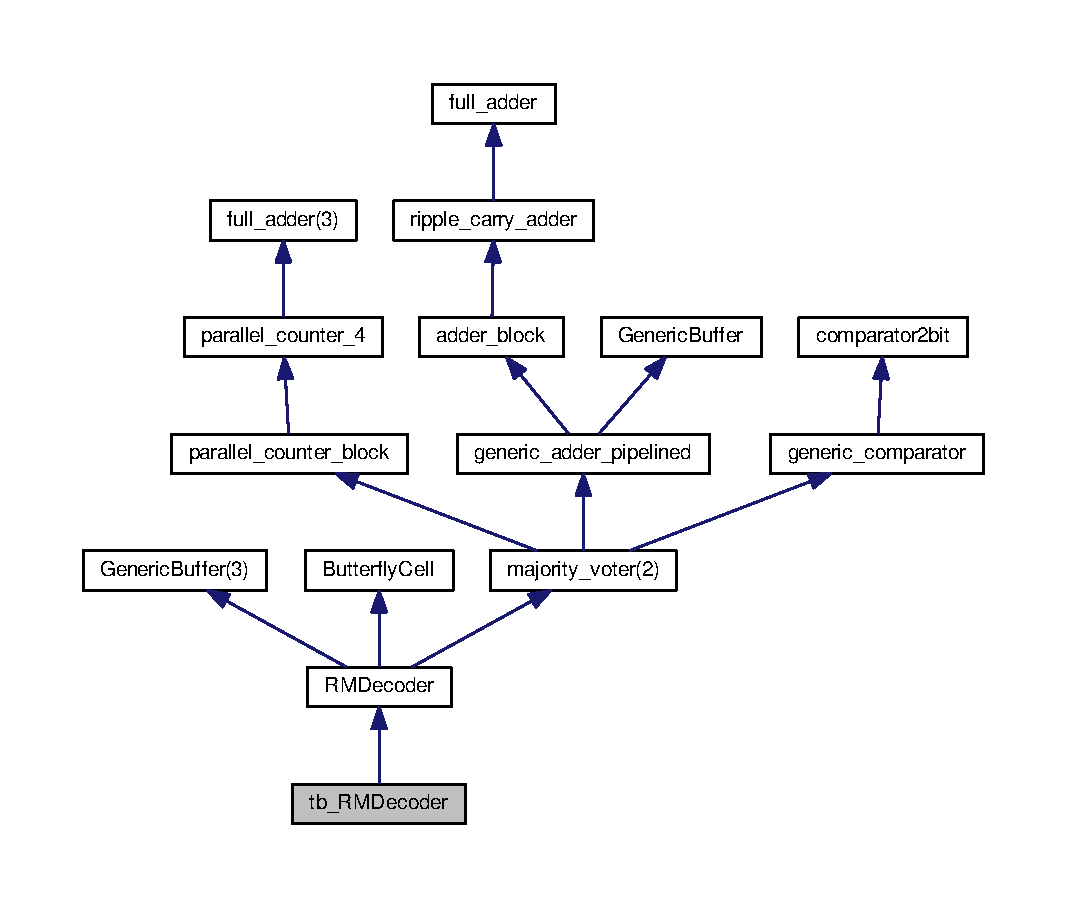
\includegraphics[width=350pt]{classtb___r_m_decoder__inherit__graph}
\end{center}
\end{figure}


Diagramma di collaborazione per tb\+\_\+\+R\+M\+Decoder\+:\nopagebreak
\begin{figure}[H]
\begin{center}
\leavevmode
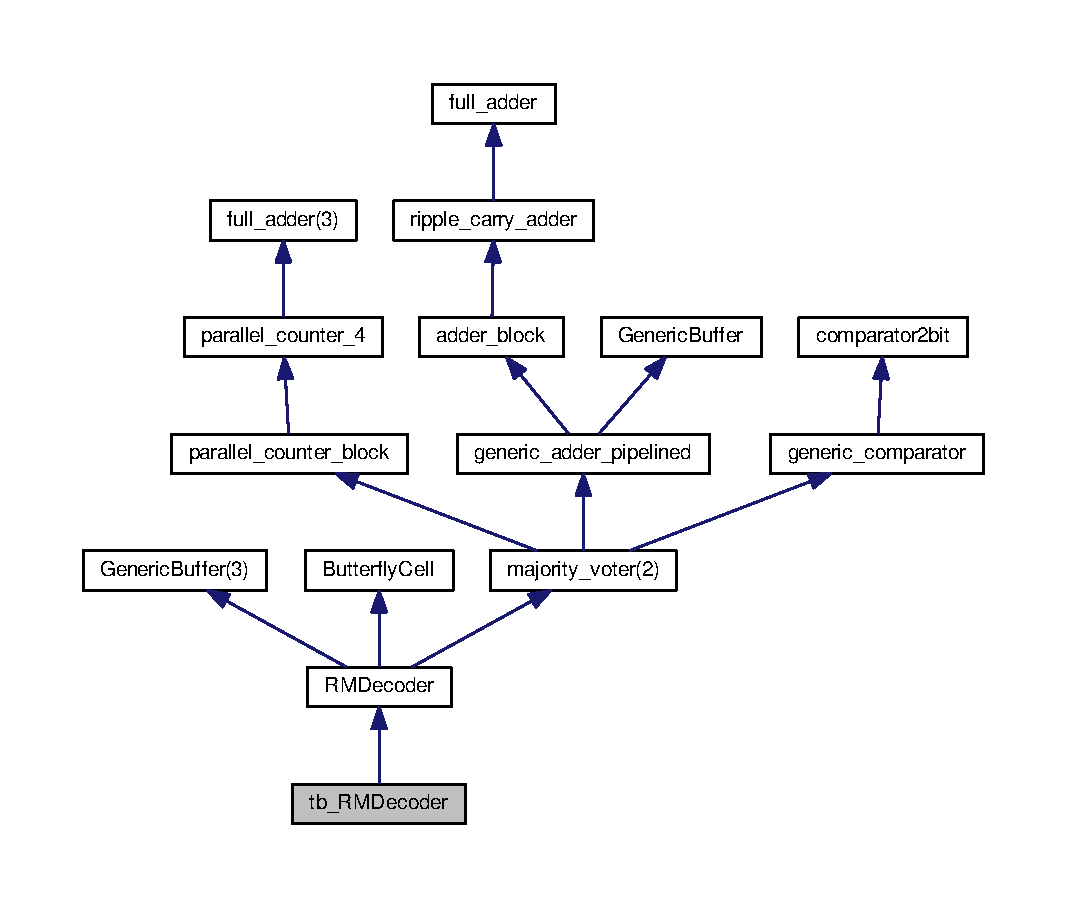
\includegraphics[width=350pt]{classtb___r_m_decoder__coll__graph}
\end{center}
\end{figure}
\subsection*{Entities}
\begin{DoxyCompactItemize}
\item 
\hyperlink{classtb___r_m_decoder_1_1_behavioral}{Behavioral} architecture
\end{DoxyCompactItemize}
\subsection*{Libraries}
 \begin{DoxyCompactItemize}
\item 
\hypertarget{classtb___r_m_decoder_a0a6af6eef40212dbaf130d57ce711256}{\hyperlink{classtb___r_m_decoder_a0a6af6eef40212dbaf130d57ce711256}{ieee} }\label{classtb___r_m_decoder_a0a6af6eef40212dbaf130d57ce711256}

\begin{DoxyCompactList}\small\item\em \+: Salvatore Barone $<$\href{mailto:salvator.barone@gmail.com}{\tt salvator.\+barone@gmail.\+com}, \href{mailto:salvator.barone@studenti.unina.it}{\tt salvator.\+barone@studenti.\+unina.\+it}$>$ \+: 03-\/05-\/2017 \+: tb\+\_\+\+R\+M\+Decoder.\+vhd \end{DoxyCompactList}\end{DoxyCompactItemize}
\subsection*{Use Clauses}
 \begin{DoxyCompactItemize}
\item 
\hypertarget{classtb___r_m_decoder_gacd03516902501cd1c7296a98e22c6fcb}{\hyperlink{group___r_m_decoder_gacd03516902501cd1c7296a98e22c6fcb}{std\+\_\+logic\+\_\+1164}   }\label{classtb___r_m_decoder_gacd03516902501cd1c7296a98e22c6fcb}

\end{DoxyCompactItemize}


La documentazione per questa classe è stata generata a partire dal seguente file\+:\begin{DoxyCompactItemize}
\item 
R\+M\+Decoder/tb\+\_\+\+R\+M\+Decoder.\+vhd\end{DoxyCompactItemize}

\hypertarget{classtb___r_m_encoder}{\section{tb\+\_\+\+R\+M\+Encoder Entity Reference}
\label{classtb___r_m_encoder}\index{tb\+\_\+\+R\+M\+Encoder@{tb\+\_\+\+R\+M\+Encoder}}
}


Diagramma delle classi per tb\+\_\+\+R\+M\+Encoder\nopagebreak
\begin{figure}[H]
\begin{center}
\leavevmode
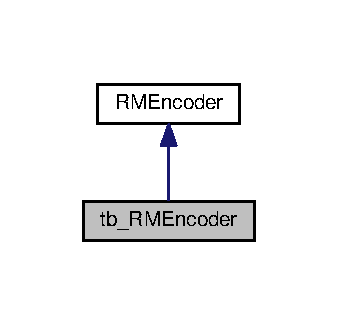
\includegraphics[width=162pt]{classtb___r_m_encoder__inherit__graph}
\end{center}
\end{figure}


Diagramma di collaborazione per tb\+\_\+\+R\+M\+Encoder\+:\nopagebreak
\begin{figure}[H]
\begin{center}
\leavevmode
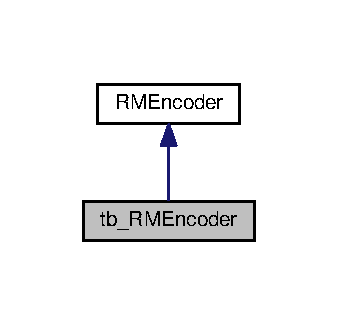
\includegraphics[width=162pt]{classtb___r_m_encoder__coll__graph}
\end{center}
\end{figure}
\subsection*{Entities}
\begin{DoxyCompactItemize}
\item 
\hyperlink{classtb___r_m_encoder_1_1_behavioral}{Behavioral} architecture
\end{DoxyCompactItemize}
\subsection*{Libraries}
 \begin{DoxyCompactItemize}
\item 
\hypertarget{classtb___r_m_encoder_ae4f03c286607f3181e16b9aa12d0c6d4}{\hyperlink{classtb___r_m_encoder_ae4f03c286607f3181e16b9aa12d0c6d4}{I\+E\+E\+E} }\label{classtb___r_m_encoder_ae4f03c286607f3181e16b9aa12d0c6d4}

\begin{DoxyCompactList}\small\item\em \+: Salvatore Barone $<$\href{mailto:salvator.barone@gmail.com}{\tt salvator.\+barone@gmail.\+com}, \href{mailto:salvator.barone@studenti.unina.it}{\tt salvator.\+barone@studenti.\+unina.\+it}$>$ \+: 03-\/05-\/2017 \+: tb\+\_\+\+R\+M\+Encoder.\+vhd \end{DoxyCompactList}\end{DoxyCompactItemize}
\subsection*{Use Clauses}
 \begin{DoxyCompactItemize}
\item 
\hypertarget{classtb___r_m_encoder_gaa4b2b25246a821511120e3149b003563}{\hyperlink{group___r_m_encoder_gaa4b2b25246a821511120e3149b003563}{S\+T\+D\+\_\+\+L\+O\+G\+I\+C\+\_\+1164}   }\label{classtb___r_m_encoder_gaa4b2b25246a821511120e3149b003563}

\item 
\hypertarget{classtb___r_m_encoder_ga2edc34402b573437d5f25fa90ba4013e}{\hyperlink{group___r_m_encoder_ga2edc34402b573437d5f25fa90ba4013e}{numeric\+\_\+std}   }\label{classtb___r_m_encoder_ga2edc34402b573437d5f25fa90ba4013e}

\end{DoxyCompactItemize}


La documentazione per questa classe è stata generata a partire dal seguente file\+:\begin{DoxyCompactItemize}
\item 
R\+M\+Encoder/tb\+\_\+\+R\+M\+Encoder.\+vhd\end{DoxyCompactItemize}

\chapter{Documentazione dei file}
\hypertarget{_butterfly_cell_8vhd}{\section{Riferimenti per il file R\+M\+Decoder/\+Butterfly\+Cell.vhd}
\label{_butterfly_cell_8vhd}\index{R\+M\+Decoder/\+Butterfly\+Cell.\+vhd@{R\+M\+Decoder/\+Butterfly\+Cell.\+vhd}}
}
\subsection*{Entities}
\begin{DoxyCompactItemize}
\item 
\hyperlink{class_butterfly_cell}{Butterfly\+Cell} entity
\begin{DoxyCompactList}\small\item\em implementazione V\+H\+D\+L dello swap usato nel decodificatore di Reed-\/\+Muller \end{DoxyCompactList}\item 
\hyperlink{class_butterfly_cell_1_1_structural}{Structural} architecture
\end{DoxyCompactItemize}


\subsection{Descrizione dettagliata}
\begin{DoxyAuthor}{Autore}
Salvatore Barone \href{mailto:salvator.barone@studenti.unina.it}{\tt salvator.\+barone@studenti.\+unina.\+it} Alfonso Di Martino \href{mailto:alf.dimartino@studenti.unina.it}{\tt alf.\+dimartino@studenti.\+unina.\+it} Pietro Liguori \href{mailto:pi.liguori@studenti.unina.it}{\tt pi.\+liguori@studenti.\+unina.\+it} 
\end{DoxyAuthor}
\begin{DoxyDate}{Data}
13 04 2017
\end{DoxyDate}
\begin{DoxyCopyright}{Copyright}
This program is free software; you can redistribute it and/or modify it under the terms of the G\+N\+U General Public License as published by the Free Software Foundation; either version 3 of the License, or any later version. This program is distributed in the hope that it will be useful, but W\+I\+T\+H\+O\+U\+T A\+N\+Y W\+A\+R\+R\+A\+N\+T\+Y; without even the implied warranty of M\+E\+R\+C\+H\+A\+N\+T\+A\+B\+I\+L\+I\+T\+Y or F\+I\+T\+N\+E\+S\+S F\+O\+R A P\+A\+R\+T\+I\+C\+U\+L\+A\+R P\+U\+R\+P\+O\+S\+E. See the G\+N\+U General Public License for more details. You should have received a copy of the G\+N\+U General Public License along with this program; if not, write to the Free Software Foundation, Inc., 51 Franklin Street, Fifth Floor, Boston, M\+A 02110-\/1301, U\+S\+A. 
\end{DoxyCopyright}

\hypertarget{adder__block_8vhd}{\section{Riferimenti per il file R\+M\+Decoder/\+Majority\+Voter/adder\+\_\+block.vhd}
\label{adder__block_8vhd}\index{R\+M\+Decoder/\+Majority\+Voter/adder\+\_\+block.\+vhd@{R\+M\+Decoder/\+Majority\+Voter/adder\+\_\+block.\+vhd}}
}
\subsection*{Entities}
\begin{DoxyCompactItemize}
\item 
\hyperlink{classadder__block}{adder\+\_\+block} entity
\begin{DoxyCompactList}\small\item\em Implementazione V\+H\+D\+L \hyperlink{classadder__block_1_1_structural}{Structural} di un generico livello del componente generic\+\_\+adder. Tale livello è costituito da 2$^\wedge$level addizionatori che lavorano in parallelo, di dimensione dipendente dal livello corrente\+: N = number\+\_\+bit\+\_\+for\+\_\+operand + log2(number\+\_\+operand)-\/level-\/1. \end{DoxyCompactList}\item 
\hyperlink{classadder__block_1_1_structural}{Structural} architecture
\end{DoxyCompactItemize}


\subsection{Descrizione dettagliata}
\begin{DoxyAuthor}{Autore}
Salvatore Barone \href{mailto:salvator.barone@studenti.unina.it}{\tt salvator.\+barone@studenti.\+unina.\+it} Alfonso Di Martino \href{mailto:alf.dimartino@studenti.unina.it}{\tt alf.\+dimartino@studenti.\+unina.\+it} Pietro Liguori \href{mailto:pi.liguori@studenti.unina.it}{\tt pi.\+liguori@studenti.\+unina.\+it} 
\end{DoxyAuthor}
\begin{DoxyDate}{Data}
15.\+04.\+2017 19\+:51\+:29
\end{DoxyDate}
\begin{DoxyCopyright}{Copyright}
This program is free software; you can redistribute it and/or modify it under the terms of the G\+N\+U General Public License as published by the Free Software Foundation; either version 3 of the License, or any later version. This program is distributed in the hope that it will be useful, but W\+I\+T\+H\+O\+U\+T A\+N\+Y W\+A\+R\+R\+A\+N\+T\+Y; without even the implied warranty of M\+E\+R\+C\+H\+A\+N\+T\+A\+B\+I\+L\+I\+T\+Y or F\+I\+T\+N\+E\+S\+S F\+O\+R A P\+A\+R\+T\+I\+C\+U\+L\+A\+R P\+U\+R\+P\+O\+S\+E. See the G\+N\+U General Public License for more details. You should have received a copy of the G\+N\+U General Public License along with this program; if not, write to the Free Software Foundation, Inc., 51 Franklin Street, Fifth Floor, Boston, M\+A 02110-\/1301, U\+S\+A. 
\end{DoxyCopyright}

\hypertarget{comparator2bit_8vhd}{\section{Riferimenti per il file R\+M\+Decoder/\+Majority\+Voter/comparator2bit.vhd}
\label{comparator2bit_8vhd}\index{R\+M\+Decoder/\+Majority\+Voter/comparator2bit.\+vhd@{R\+M\+Decoder/\+Majority\+Voter/comparator2bit.\+vhd}}
}
\subsection*{Entities}
\begin{DoxyCompactItemize}
\item 
\hyperlink{classcomparator2bit}{comparator2bit} entity
\begin{DoxyCompactList}\small\item\em Implementazione V\+H\+D\+L Data Flow di un comparatore a 2 bit che tiene conto anche del risutato di un confronto precedente. \end{DoxyCompactList}\item 
\hyperlink{classcomparator2bit_1_1_data_flow}{Data\+Flow} architecture
\end{DoxyCompactItemize}


\subsection{Descrizione dettagliata}
\begin{DoxyAuthor}{Autore}
Salvatore Barone \href{mailto:salvator.barone@studenti.unina.it}{\tt salvator.\+barone@studenti.\+unina.\+it} Alfonso Di Martino \href{mailto:alf.dimartino@studenti.unina.it}{\tt alf.\+dimartino@studenti.\+unina.\+it} Pietro Liguori \href{mailto:pi.liguori@studenti.unina.it}{\tt pi.\+liguori@studenti.\+unina.\+it} 
\end{DoxyAuthor}
\begin{DoxyDate}{Data}
13.\+04.\+2017 20\+:27\+:06
\end{DoxyDate}
\begin{DoxyCopyright}{Copyright}
This program is free software; you can redistribute it and/or modify it under the terms of the G\+N\+U General Public License as published by the Free Software Foundation; either version 3 of the License, or any later version. This program is distributed in the hope that it will be useful, but W\+I\+T\+H\+O\+U\+T A\+N\+Y W\+A\+R\+R\+A\+N\+T\+Y; without even the implied warranty of M\+E\+R\+C\+H\+A\+N\+T\+A\+B\+I\+L\+I\+T\+Y or F\+I\+T\+N\+E\+S\+S F\+O\+R A P\+A\+R\+T\+I\+C\+U\+L\+A\+R P\+U\+R\+P\+O\+S\+E. See the G\+N\+U General Public License for more details. You should have received a copy of the G\+N\+U General Public License along with this program; if not, write to the Free Software Foundation, Inc., 51 Franklin Street, Fifth Floor, Boston, M\+A 02110-\/1301, U\+S\+A. 
\end{DoxyCopyright}

\hypertarget{full__adder_8vhd}{\section{Riferimenti per il file R\+M\+Decoder/\+Majority\+Voter/full\+\_\+adder.vhd}
\label{full__adder_8vhd}\index{R\+M\+Decoder/\+Majority\+Voter/full\+\_\+adder.\+vhd@{R\+M\+Decoder/\+Majority\+Voter/full\+\_\+adder.\+vhd}}
}
\subsection*{Entities}
\begin{DoxyCompactItemize}
\item 
\hyperlink{classfull__adder}{full\+\_\+adder} entity
\item 
\hyperlink{classfull__adder_1_1_data_flow}{Data\+Flow} architecture
\end{DoxyCompactItemize}


\subsection{Descrizione dettagliata}
\begin{DoxyAuthor}{Autore}
Salvatore Barone \href{mailto:salvator.barone@studenti.unina.it}{\tt salvator.\+barone@studenti.\+unina.\+it} Alfonso Di Martino \href{mailto:alf.dimartino@studenti.unina.it}{\tt alf.\+dimartino@studenti.\+unina.\+it} Pietro Liguori \href{mailto:pi.liguori@studenti.unina.it}{\tt pi.\+liguori@studenti.\+unina.\+it} 
\end{DoxyAuthor}
\begin{DoxyDate}{Data}
12/19/2015 17\+:27\+:35
\end{DoxyDate}
\begin{DoxyCopyright}{Copyright}
This program is free software; you can redistribute it and/or modify it under the terms of the G\+N\+U General Public License as published by the Free Software Foundation; either version 3 of the License, or any later version. This program is distributed in the hope that it will be useful, but W\+I\+T\+H\+O\+U\+T A\+N\+Y W\+A\+R\+R\+A\+N\+T\+Y; without even the implied warranty of M\+E\+R\+C\+H\+A\+N\+T\+A\+B\+I\+L\+I\+T\+Y or F\+I\+T\+N\+E\+S\+S F\+O\+R A P\+A\+R\+T\+I\+C\+U\+L\+A\+R P\+U\+R\+P\+O\+S\+E. See the G\+N\+U General Public License for more details. You should have received a copy of the G\+N\+U General Public License along with this program; if not, write to the Free Software Foundation, Inc., 51 Franklin Street, Fifth Floor, Boston, M\+A 02110-\/1301, U\+S\+A. 
\end{DoxyCopyright}

\hypertarget{generic__adder__pipelined_8vhd}{\section{Riferimenti per il file R\+M\+Decoder/\+Majority\+Voter/generic\+\_\+adder\+\_\+pipelined.vhd}
\label{generic__adder__pipelined_8vhd}\index{R\+M\+Decoder/\+Majority\+Voter/generic\+\_\+adder\+\_\+pipelined.\+vhd@{R\+M\+Decoder/\+Majority\+Voter/generic\+\_\+adder\+\_\+pipelined.\+vhd}}
}
\subsection*{Entities}
\begin{DoxyCompactItemize}
\item 
\hyperlink{classgeneric__adder__pipelined}{generic\+\_\+adder\+\_\+pipelined} entity
\begin{DoxyCompactList}\small\item\em Implementazione V\+H\+D\+L \hyperlink{classgeneric__adder__pipelined_1_1_structural}{Structural} di un addizionatore generico pipelined \+: M operandi di N bit. \end{DoxyCompactList}\item 
\hyperlink{classgeneric__adder__pipelined_1_1_structural}{Structural} architecture
\end{DoxyCompactItemize}


\subsection{Descrizione dettagliata}
\begin{DoxyAuthor}{Autore}
Salvatore Barone \href{mailto:salvator.barone@studenti.unina.it}{\tt salvator.\+barone@studenti.\+unina.\+it} Alfonso Di Martino \href{mailto:alf.dimartino@studenti.unina.it}{\tt alf.\+dimartino@studenti.\+unina.\+it} Pietro Liguori \href{mailto:pi.liguori@studenti.unina.it}{\tt pi.\+liguori@studenti.\+unina.\+it} 
\end{DoxyAuthor}
\begin{DoxyDate}{Data}
15.\+04.\+2017 11\+:59\+:47
\end{DoxyDate}
\begin{DoxyCopyright}{Copyright}
This program is free software; you can redistribute it and/or modify it under the terms of the G\+N\+U General Public License as published by the Free Software Foundation; either version 3 of the License, or any later version. This program is distributed in the hope that it will be useful, but W\+I\+T\+H\+O\+U\+T A\+N\+Y W\+A\+R\+R\+A\+N\+T\+Y; without even the implied warranty of M\+E\+R\+C\+H\+A\+N\+T\+A\+B\+I\+L\+I\+T\+Y or F\+I\+T\+N\+E\+S\+S F\+O\+R A P\+A\+R\+T\+I\+C\+U\+L\+A\+R P\+U\+R\+P\+O\+S\+E. See the G\+N\+U General Public License for more details. You should have received a copy of the G\+N\+U General Public License along with this program; if not, write to the Free Software Foundation, Inc., 51 Franklin Street, Fifth Floor, Boston, M\+A 02110-\/1301, U\+S\+A. 
\end{DoxyCopyright}

\hypertarget{generic__comparator_8vhd}{\section{Riferimenti per il file R\+M\+Decoder/\+Majority\+Voter/generic\+\_\+comparator.vhd}
\label{generic__comparator_8vhd}\index{R\+M\+Decoder/\+Majority\+Voter/generic\+\_\+comparator.\+vhd@{R\+M\+Decoder/\+Majority\+Voter/generic\+\_\+comparator.\+vhd}}
}
\subsection*{Entities}
\begin{DoxyCompactItemize}
\item 
\hyperlink{classgeneric__comparator}{generic\+\_\+comparator} entity
\begin{DoxyCompactList}\small\item\em Implementazione V\+H\+D\+L \hyperlink{classgeneric__comparator_1_1_structural}{Structural} di un generico comparatore a maggioranza di due stringhe di width bit. Tale implementazione genera una catena di \char`\"{}width\char`\"{} comparatori a 2 bit. \end{DoxyCompactList}\item 
\hyperlink{classgeneric__comparator_1_1_structural}{Structural} architecture
\end{DoxyCompactItemize}


\subsection{Descrizione dettagliata}
\begin{DoxyAuthor}{Autore}
Salvatore Barone \href{mailto:salvator.barone@studenti.unina.it}{\tt salvator.\+barone@studenti.\+unina.\+it} Alfonso Di Martino \href{mailto:alf.dimartino@studenti.unina.it}{\tt alf.\+dimartino@studenti.\+unina.\+it} Pietro Liguori \href{mailto:pi.liguori@studenti.unina.it}{\tt pi.\+liguori@studenti.\+unina.\+it} 
\end{DoxyAuthor}
\begin{DoxyDate}{Data}
13.\+04.\+2017 20\+:27\+:06
\end{DoxyDate}
\begin{DoxyCopyright}{Copyright}
This program is free software; you can redistribute it and/or modify it under the terms of the G\+N\+U General Public License as published by the Free Software Foundation; either version 3 of the License, or any later version. This program is distributed in the hope that it will be useful, but W\+I\+T\+H\+O\+U\+T A\+N\+Y W\+A\+R\+R\+A\+N\+T\+Y; without even the implied warranty of M\+E\+R\+C\+H\+A\+N\+T\+A\+B\+I\+L\+I\+T\+Y or F\+I\+T\+N\+E\+S\+S F\+O\+R A P\+A\+R\+T\+I\+C\+U\+L\+A\+R P\+U\+R\+P\+O\+S\+E. See the G\+N\+U General Public License for more details. You should have received a copy of the G\+N\+U General Public License along with this program; if not, write to the Free Software Foundation, Inc., 51 Franklin Street, Fifth Floor, Boston, M\+A 02110-\/1301, U\+S\+A. 
\end{DoxyCopyright}

\hypertarget{majority__voter_8vhd}{\section{Riferimenti per il file R\+M\+Decoder/\+Majority\+Voter/majority\+\_\+voter.vhd}
\label{majority__voter_8vhd}\index{R\+M\+Decoder/\+Majority\+Voter/majority\+\_\+voter.\+vhd@{R\+M\+Decoder/\+Majority\+Voter/majority\+\_\+voter.\+vhd}}
}
\subsection*{Entities}
\begin{DoxyCompactItemize}
\item 
\hyperlink{classmajority__voter}{majority\+\_\+voter} entity
\begin{DoxyCompactList}\small\item\em Implementazione V\+H\+D\+L \hyperlink{classmajority__voter_1_1_structural}{Structural} del majority voter. \end{DoxyCompactList}\item 
\hyperlink{classmajority__voter_1_1_structural}{Structural} architecture
\end{DoxyCompactItemize}


\subsection{Descrizione dettagliata}
\begin{DoxyAuthor}{Autore}
Salvatore Barone \href{mailto:salvator.barone@studenti.unina.it}{\tt salvator.\+barone@studenti.\+unina.\+it} Alfonso Di Martino \href{mailto:alf.dimartino@studenti.unina.it}{\tt alf.\+dimartino@studenti.\+unina.\+it} Pietro Liguori \href{mailto:pi.liguori@studenti.unina.it}{\tt pi.\+liguori@studenti.\+unina.\+it} 
\end{DoxyAuthor}
\begin{DoxyDate}{Data}
14.\+04.\+2017 00\+:12\+:12
\end{DoxyDate}
\begin{DoxyCopyright}{Copyright}
This program is free software; you can redistribute it and/or modify it under the terms of the G\+N\+U General Public License as published by the Free Software Foundation; either version 3 of the License, or any later version. This program is distributed in the hope that it will be useful, but W\+I\+T\+H\+O\+U\+T A\+N\+Y W\+A\+R\+R\+A\+N\+T\+Y; without even the implied warranty of M\+E\+R\+C\+H\+A\+N\+T\+A\+B\+I\+L\+I\+T\+Y or F\+I\+T\+N\+E\+S\+S F\+O\+R A P\+A\+R\+T\+I\+C\+U\+L\+A\+R P\+U\+R\+P\+O\+S\+E. See the G\+N\+U General Public License for more details. You should have received a copy of the G\+N\+U General Public License along with this program; if not, write to the Free Software Foundation, Inc., 51 Franklin Street, Fifth Floor, Boston, M\+A 02110-\/1301, U\+S\+A. 
\end{DoxyCopyright}

\hypertarget{parallel__counter__4_8vhd}{\section{Riferimenti per il file R\+M\+Decoder/\+Majority\+Voter/parallel\+\_\+counter\+\_\+4.vhd}
\label{parallel__counter__4_8vhd}\index{R\+M\+Decoder/\+Majority\+Voter/parallel\+\_\+counter\+\_\+4.\+vhd@{R\+M\+Decoder/\+Majority\+Voter/parallel\+\_\+counter\+\_\+4.\+vhd}}
}
\subsection*{Entities}
\begin{DoxyCompactItemize}
\item 
\hyperlink{classparallel__counter__4}{parallel\+\_\+counter\+\_\+4} entity
\item 
\hyperlink{classparallel__counter__4_1_1_structural}{Structural} architecture
\end{DoxyCompactItemize}


\subsection{Descrizione dettagliata}
\begin{DoxyAuthor}{Autore}
Salvatore Barone \href{mailto:salvator.barone@studenti.unina.it}{\tt salvator.\+barone@studenti.\+unina.\+it} Alfonso Di Martino \href{mailto:alf.dimartino@studenti.unina.it}{\tt alf.\+dimartino@studenti.\+unina.\+it} Pietro Liguori \href{mailto:pi.liguori@studenti.unina.it}{\tt pi.\+liguori@studenti.\+unina.\+it} 
\end{DoxyAuthor}
\begin{DoxyDate}{Data}
12/19/2015 17\+:27\+:35
\end{DoxyDate}
\begin{DoxyCopyright}{Copyright}
This program is free software; you can redistribute it and/or modify it under the terms of the G\+N\+U General Public License as published by the Free Software Foundation; either version 3 of the License, or any later version. This program is distributed in the hope that it will be useful, but W\+I\+T\+H\+O\+U\+T A\+N\+Y W\+A\+R\+R\+A\+N\+T\+Y; without even the implied warranty of M\+E\+R\+C\+H\+A\+N\+T\+A\+B\+I\+L\+I\+T\+Y or F\+I\+T\+N\+E\+S\+S F\+O\+R A P\+A\+R\+T\+I\+C\+U\+L\+A\+R P\+U\+R\+P\+O\+S\+E. See the G\+N\+U General Public License for more details. You should have received a copy of the G\+N\+U General Public License along with this program; if not, write to the Free Software Foundation, Inc., 51 Franklin Street, Fifth Floor, Boston, M\+A 02110-\/1301, U\+S\+A. 
\end{DoxyCopyright}

\hypertarget{parallel__counter__block_8vhd}{\section{Riferimenti per il file R\+M\+Decoder/\+Majority\+Voter/parallel\+\_\+counter\+\_\+block.vhd}
\label{parallel__counter__block_8vhd}\index{R\+M\+Decoder/\+Majority\+Voter/parallel\+\_\+counter\+\_\+block.\+vhd@{R\+M\+Decoder/\+Majority\+Voter/parallel\+\_\+counter\+\_\+block.\+vhd}}
}
\subsection*{Entities}
\begin{DoxyCompactItemize}
\item 
\hyperlink{classparallel__counter__block}{parallel\+\_\+counter\+\_\+block} entity
\begin{DoxyCompactList}\small\item\em Implementazione V\+H\+D\+L \hyperlink{classparallel__counter__block_1_1_structural}{Structural} del Modulo 1 \+: genera width/4 contatori paralleli a 4 bit. Data una stringa di input di width bit, multipla di 4, assegna a ogni contatore un nibble. Ogni contatore parallelo a 4 bit codifica in binario il numero di 1 presente nel nibble di competenza. \end{DoxyCompactList}\item 
\hyperlink{classparallel__counter__block_1_1_structural}{Structural} architecture
\end{DoxyCompactItemize}


\subsection{Descrizione dettagliata}
\begin{DoxyAuthor}{Autore}
Salvatore Barone \href{mailto:salvator.barone@studenti.unina.it}{\tt salvator.\+barone@studenti.\+unina.\+it} Alfonso Di Martino \href{mailto:alf.dimartino@studenti.unina.it}{\tt alf.\+dimartino@studenti.\+unina.\+it} Pietro Liguori \href{mailto:pi.liguori@studenti.unina.it}{\tt pi.\+liguori@studenti.\+unina.\+it} 
\end{DoxyAuthor}
\begin{DoxyDate}{Data}
14.\+04.\+2017 00\+:32\+:13
\end{DoxyDate}
\begin{DoxyCopyright}{Copyright}
This program is free software; you can redistribute it and/or modify it under the terms of the G\+N\+U General Public License as published by the Free Software Foundation; either version 3 of the License, or any later version. This program is distributed in the hope that it will be useful, but W\+I\+T\+H\+O\+U\+T A\+N\+Y W\+A\+R\+R\+A\+N\+T\+Y; without even the implied warranty of M\+E\+R\+C\+H\+A\+N\+T\+A\+B\+I\+L\+I\+T\+Y or F\+I\+T\+N\+E\+S\+S F\+O\+R A P\+A\+R\+T\+I\+C\+U\+L\+A\+R P\+U\+R\+P\+O\+S\+E. See the G\+N\+U General Public License for more details. You should have received a copy of the G\+N\+U General Public License along with this program; if not, write to the Free Software Foundation, Inc., 51 Franklin Street, Fifth Floor, Boston, M\+A 02110-\/1301, U\+S\+A. 
\end{DoxyCopyright}

\hypertarget{ripple__carry__adder_8vhd}{\section{Riferimenti per il file R\+M\+Decoder/\+Majority\+Voter/ripple\+\_\+carry\+\_\+adder.vhd}
\label{ripple__carry__adder_8vhd}\index{R\+M\+Decoder/\+Majority\+Voter/ripple\+\_\+carry\+\_\+adder.\+vhd@{R\+M\+Decoder/\+Majority\+Voter/ripple\+\_\+carry\+\_\+adder.\+vhd}}
}
\subsection*{Entities}
\begin{DoxyCompactItemize}
\item 
\hyperlink{classripple__carry__adder}{ripple\+\_\+carry\+\_\+adder} entity
\begin{DoxyCompactList}\small\item\em Implementazione V\+H\+D\+L Structural di un Ripple Carry Adder generico a N bit. \end{DoxyCompactList}\item 
\hyperlink{classripple__carry__adder_1_1structural}{structural} architecture
\end{DoxyCompactItemize}


\subsection{Descrizione dettagliata}
\begin{DoxyAuthor}{Autore}
Salvatore Barone \href{mailto:salvator.barone@studenti.unina.it}{\tt salvator.\+barone@studenti.\+unina.\+it} Alfonso Di Martino \href{mailto:alf.dimartino@studenti.unina.it}{\tt alf.\+dimartino@studenti.\+unina.\+it} Pietro Liguori \href{mailto:pi.liguori@studenti.unina.it}{\tt pi.\+liguori@studenti.\+unina.\+it} 
\end{DoxyAuthor}
\begin{DoxyDate}{Data}
19.\+12.\+2015 17\+:27\+:35
\end{DoxyDate}
\begin{DoxyCopyright}{Copyright}
This program is free software; you can redistribute it and/or modify it under the terms of the G\+N\+U General Public License as published by the Free Software Foundation; either version 3 of the License, or any later version. This program is distributed in the hope that it will be useful, but W\+I\+T\+H\+O\+U\+T A\+N\+Y W\+A\+R\+R\+A\+N\+T\+Y; without even the implied warranty of M\+E\+R\+C\+H\+A\+N\+T\+A\+B\+I\+L\+I\+T\+Y or F\+I\+T\+N\+E\+S\+S F\+O\+R A P\+A\+R\+T\+I\+C\+U\+L\+A\+R P\+U\+R\+P\+O\+S\+E. See the G\+N\+U General Public License for more details. You should have received a copy of the G\+N\+U General Public License along with this program; if not, write to the Free Software Foundation, Inc., 51 Franklin Street, Fifth Floor, Boston, M\+A 02110-\/1301, U\+S\+A. 
\end{DoxyCopyright}

\hypertarget{_r_m_decoder_8vhd}{\section{Riferimenti per il file R\+M\+Decoder/\+R\+M\+Decoder.vhd}
\label{_r_m_decoder_8vhd}\index{R\+M\+Decoder/\+R\+M\+Decoder.\+vhd@{R\+M\+Decoder/\+R\+M\+Decoder.\+vhd}}
}
\subsection*{Entities}
\begin{DoxyCompactItemize}
\item 
\hyperlink{class_r_m_decoder}{R\+M\+Decoder} entity
\begin{DoxyCompactList}\small\item\em Implementazione V\+H\+D\+L del decodificatore per codici di Reed-\/\+Muller(1,m) \end{DoxyCompactList}\item 
\hyperlink{class_r_m_decoder_1_1_structural}{Structural} architecture
\end{DoxyCompactItemize}


\subsection{Descrizione dettagliata}
\begin{DoxyAuthor}{Autore}
Salvatore Barone \href{mailto:salvator.barone@studenti.unina.it}{\tt salvator.\+barone@studenti.\+unina.\+it} Alfonso Di Martino \href{mailto:alf.dimartino@studenti.unina.it}{\tt alf.\+dimartino@studenti.\+unina.\+it} Pietro Liguori \href{mailto:pi.liguori@studenti.unina.it}{\tt pi.\+liguori@studenti.\+unina.\+it} 
\end{DoxyAuthor}
\begin{DoxyDate}{Data}
13-\/04-\/2017
\begin{DoxyItemize}
\item implementazione V\+H\+D\+L del decodificatore a maggioranza utilizzabile per la decodifica dei codici di Reed-\/\+Muller R\+M(1, m). 
\end{DoxyItemize}
\end{DoxyDate}
\begin{DoxyCopyright}{Copyright}
This program is free software; you can redistribute it and/or modify it under the terms of the G\+N\+U General Public License as published by the Free Software Foundation; either version 3 of the License, or any later version. This program is distributed in the hope that it will be useful, but W\+I\+T\+H\+O\+U\+T A\+N\+Y W\+A\+R\+R\+A\+N\+T\+Y; without even the implied warranty of M\+E\+R\+C\+H\+A\+N\+T\+A\+B\+I\+L\+I\+T\+Y or F\+I\+T\+N\+E\+S\+S F\+O\+R A P\+A\+R\+T\+I\+C\+U\+L\+A\+R P\+U\+R\+P\+O\+S\+E. See the G\+N\+U General Public License for more details. You should have received a copy of the G\+N\+U General Public License along with this program; if not, write to the Free Software Foundation, Inc., 51 Franklin Street, Fifth Floor, Boston, M\+A 02110-\/1301, U\+S\+A. 
\end{DoxyCopyright}

\hypertarget{_r_m_encoder_8vhd}{\section{Riferimenti per il file R\+M\+Encoder/\+R\+M\+Encoder.vhd}
\label{_r_m_encoder_8vhd}\index{R\+M\+Encoder/\+R\+M\+Encoder.\+vhd@{R\+M\+Encoder/\+R\+M\+Encoder.\+vhd}}
}
\subsection*{Entities}
\begin{DoxyCompactItemize}
\item 
\hyperlink{class_r_m_encoder}{R\+M\+Encoder} entity
\begin{DoxyCompactList}\small\item\em Implementazione V\+H\+D\+L del codificatore per codici di Reed-\/\+Muller(1,m) \end{DoxyCompactList}\item 
\hyperlink{class_r_m_encoder_1_1_structural}{Structural} architecture
\end{DoxyCompactItemize}


\subsection{Descrizione dettagliata}
\begin{DoxyAuthor}{Autore}
Salvatore Barone \href{mailto:salvator.barone@studenti.unina.it}{\tt salvator.\+barone@studenti.\+unina.\+it} Alfonso Di Martino \href{mailto:alf.dimartino@studenti.unina.it}{\tt alf.\+dimartino@studenti.\+unina.\+it} Pietro Liguori \href{mailto:pi.liguori@studenti.unina.it}{\tt pi.\+liguori@studenti.\+unina.\+it} 
\end{DoxyAuthor}
\begin{DoxyDate}{Data}
13-\/04-\/2017
\begin{DoxyItemize}
\item implementazione V\+H\+D\+L del codificatore utilizzabile per la codifica dei codici di Reed-\/\+Muller R\+M(1, m). 
\end{DoxyItemize}
\end{DoxyDate}
\begin{DoxyCopyright}{Copyright}
This program is free software; you can redistribute it and/or modify it under the terms of the G\+N\+U General Public License as published by the Free Software Foundation; either version 3 of the License, or any later version. This program is distributed in the hope that it will be useful, but W\+I\+T\+H\+O\+U\+T A\+N\+Y W\+A\+R\+R\+A\+N\+T\+Y; without even the implied warranty of M\+E\+R\+C\+H\+A\+N\+T\+A\+B\+I\+L\+I\+T\+Y or F\+I\+T\+N\+E\+S\+S F\+O\+R A P\+A\+R\+T\+I\+C\+U\+L\+A\+R P\+U\+R\+P\+O\+S\+E. See the G\+N\+U General Public License for more details. You should have received a copy of the G\+N\+U General Public License along with this program; if not, write to the Free Software Foundation, Inc., 51 Franklin Street, Fifth Floor, Boston, M\+A 02110-\/1301, U\+S\+A. 
\end{DoxyCopyright}

%--- End generated contents ---

% Index
\newpage
\phantomsection
\addcontentsline{toc}{chapter}{Indice}
\printindex

\end{document}
